\documentclass[a4paper,11pt,nocenter,bold,notitlepage,noheadline,noindent]{
thesis}
\usepackage{etex} % Fix problem of running out of dimensions
%                     PACKAGES
% Add any additional packages that you require to the list below
%
\usepackage{a4,natbib}
\usepackage[dvips]{graphicx}
\usepackage{mathtools, amssymb}
\usepackage{float}
%\usepackage[lined,boxed,commentsnumbered]{algorithm2e}
\usepackage{subfigure}
\usepackage{tabularx}
\usepackage{tabulary}
\newcolumntype{K}[1]{>{\centering\arraybackslash}p{#1}}
\usepackage[ruled,vlined]{algorithm2e}
%\usepackage{algorithm}
%\usepackage{algorithmic}
\usepackage{algpseudocode}
\usepackage{listings}
\usepackage{tikz}
\usetikzlibrary{arrows, shapes, trees, backgrounds, calc}
\usepackage[hidelinks]{hyperref}
\usepackage{breakurl}

\usepackage{setspace}
\usepackage{bold-extra}
\usepackage{geometry}
%                     SPACING
% This really shouldn't be necessary...
\usepackage{setspace}
\onehalfspacing
% \doublespacing
\setcounter{secnumdepth}{5}

%                     DOCUMENT DETAILS
% Edit these entries to fit your document
%

\newcommand{\theauthor}{NEIL ELIOT}
\newcommand{\thetitle}{METHODS FOR THE EFFICIENT DEPLOYMENT AND COORDINATION OF SWARM ROBOTIC SYSTEMS}
\newcommand{\thedegreeshort}{PhD}
\newcommand{\thedegreelong}{Doctor of Philosophy}
\newcommand{\themonth}{January}
\newcommand{\theyear}{2017}
\newcommand{\subsubsubsection}[1]{\medskip\par\emph{#1:}}
\newcommand{\swarmA}{Hexagonal}
\newcommand{\swarmB}{Connected}
\newcommand{\stability}{internal movement}
\newcommand{\Stability}{Internal movement}
\newcommand*\circled[1]{\tikz[baseline=(char.base)]{
            \node[shape=circle,draw,inner sep=2pt] (char) {#1};}}
\def\HiLi{\leavevmode\rlap{\hbox to \hsize{\color{yellow!50}\leaders\hrule height .8\baselineskip depth .5ex\hfill}}}
%\newcommand{\Fig}{fig.}
%\newcommand{\Figs}{figs.}
%\newcommand{\Eq}{Eq.}
%\newcommand{\eq}{eq.}
%\newcommand{\Eqs}{eqs.}
%\newcommand{\Sec}{sec.}
%\newcommand{\Alg}{alg.}
%\newcommand{\Tab}{tab.}
%\newcommand{\Tabs}{tabs.}
%\newcommand{\List}{list.}
%\newcommand{\Lists}{lists.}
%\newcommand{\Chapter}{Ch.}
\newcommand{\app}{Appendix}
\renewcommand{\chapterautorefname}{\S}
\renewcommand{\sectionautorefname}{\S}
\renewcommand{\subsectionautorefname}{\S}
\renewcommand{\subsubsectionautorefname}{\S}
\newcommand{\card}[1]{\vert{#1}\vert}
\newcommand{\magn}[1]{\Vert{#1}\Vert}
%                    DEDICATION (OPTIONAL)
%
\dedication{To my Mother for encouraging me to `Keep On Learning'}

%                     INCLUDE ONLY
% Use this if you want to process only a small part of the document

%\includeonly{CHAPTER-1/text}

%                     DOCUMENT

\begin{document}
\frontmatter

\thispagestyle{empty}
\begin{Huge}
\bfseries
\begin{center}
\thetitle

\vfill

\begin{figure}[H]
\begin{center}

\includegraphics[width=6cm]{FRONT/northumbria}
\end{center}
\end{figure}

\vfill

\theauthor

\vfill

\thedegreeshort

\vfill

\theyear
\end{center}
\end{Huge}

%\maketitle
\thispagestyle{empty}
\begin{Huge}
\onehalfspacing

\begin{center}
\textbf{\thetitle} 

\vfill

\textbf{\theauthor}

\vfill

\begin{huge}
A thesis submitted in partial fulfilment \\ of the requirements of the \\
University of Northumbria at Newcastle \\ for the degree of \\ \thedegreelong

\vfill 

Research undertaken in the Faculty of Engineering and Environment
\end{huge}

\vfill

\textbf{\themonth\ \theyear}
\end{center}
\end{Huge}

%% \begin{abstract}
%% \vspace*{-3em}
%% VERSION 1
%% 
%% Swarming has been identified in many species including fish, birds, insects and mammals. Studies of swarms has lead to many mathematical models based on robotic `agents' to mimic those behaviours and solve problems in a novel way.
%% 
%% Swarms by their construction provide redundancy through distribution of resources. There are also benefits in behaviours that manifest from simple distributed algorithms. Swarming, however, introduces complications; how do you efficiently coordinate a swarm as an infrastructure?
%% 
%% This thesis focuses on how a swarm of an arbitrary size can be coordinated using only localised sensing information and no communications infrastructure leading to a reduction in energy and resource demands.
%% 
%% This thesis presents two new coordination algorithms to coordinate a swarm's directional bias. The algorithms provide partial detection and a full detection of perimeter edges. The full perimeter detection algorithm also provides an emergent behaviour of `void closing' to create a healing effect and object surrounding.
%% 
%% To measure and compare the coordination algorithms and swarm structures this thesis proposes a new metric for measuring the `quality' of a swarms structure based upon the resultant magnitudes of inter-agent interactions. 
%% 
%% The metric and all the behaviours have been modelled and examined in a simulation environment and it can be shown that efficiencies can be obtained with the new algorithms along with improved coordination. A video demonstrating the simulator is available at: 
%% 
%% \noindent{\footnotesize\texttt{\url{https://drive.google.com/file/d/0B0DIRBx-V-eYT3YzTU03LW1pb1E/view?usp=sharing}}}
%% 
%% \newpage
%% VERSION 2
%% 
%% Swarming has been identified in many species including fish, birds, insects and mammals. Studies of swarms has lead to many mathematical models based on robotic `agents' to mimic those behaviours and solve problems in a novel way.
%% 
%% Swarms by their construction provide redundancy through distribution of resources. There are also benefits in behaviours that manifest from simple distributed algorithms. Swarming, however, introduces complications; how do you efficiently coordinate a swarm as an infrastructure and how do we identify if a swarm is operating efficiently?
%% 
%% This thesis focuses on the coordination of arbitrary sized swarms using localised sensing information that does not require a communications infrastructure. This leads to a reduction in energy and resource demands. The thesis also focuses on a new metric that allows the internal structure of a swarm to be analysed to identify efficiencies in agent movement.
%% 
%% The metric and all the behaviours have been modelled in a simulation environment. The simulator has been developed as part of this thesis and is designed to allow aspects of a swarms construct and the algorithms effects to be captured. A video demonstrating the simulator is available at: 
%% 
%% \noindent{\footnotesize\texttt{\url{https://drive.google.com/file/d/0B0DIRBx-V-eYT3YzTU03LW1pb1E/view?usp=sharing}}}
%% 
%% This thesis proposes that it is possible to coordinate arbitrary sized warms using the new techniques and algorithms, and that by using the metric that has been defined in this thesis, it is possible to identify efficiencies in the coordination of a swarm. This thesis also demonstrates that it is possible to identify the benefits of emergent behaviours and the effects the emergent behaviours have upon the swarms structure.
%% 
%% 
%% \newpage
%% VERSION 3
%% 
%% Swarming has been identified in many species including fish, birds, insects and mammals. In 1987 Craig Reynolds published his paper on boid-based swarming which has lead to many researchers creating mathematical models to enable robotic `agents' to mimic those behaviours. These behaviours have then been applied to solving problems in novel ways. Swarm based reconnaissance soon after became a topic of interest to the military and more recently in 2016 an article in Wired (www.wired.co.uk) discusses the implications of the US Navy's LOCUST (\textit{L}ow \textit{C}ost \textit{U}av \textit{S}warm \textit{T}echnology) project which uses swarms of drones specifically to create a platform capable of reconfiguring its structure in the event of failures.
%% 
%% Swarms by their construction provide redundancy through distribution of tasks and replication of resources in agents. There are also benefits in behaviours that manifest from simple distributed algorithms. However swarming introduces complications; How do you efficiently coordinate a swarm as an infrastructure and how do we identify if a swarm is operating efficiently? `Efficiency' is the ability of the swarm to use minimal resources for maximum execution of a task i.e. increasing the distance a swarm can travel or reducing the time required to carry out a task.
%% 
%% This thesis focuses on the coordination of arbitrary sized swarms using localised sensing information that does not require a communications infrastructure. This leads to a reduction in energy and resource demands. The thesis also focuses on a new metric that allows the internal structure of a swarm to be analysed to identify efficiencies in agent movement.
%% 
%% This thesis also identifies and enhances a swarms capabilities through the introduction of perimeter detection to develop emergent behaviours. Perimeter detections allows a swarm to be coordinated efficiently with a directional bias and also allows a swarm to exhibit a self-healing feature to remove voids. The self healing behaviour can be applied to ensuring the construct of a swarm is uniform and improve the area coverage of a reconnaissance task. 
%% 
%% The metric and all the behaviours have been modelled in a simulation environment. The simulator has been developed as part of this thesis and is designed to allow aspects of a swarms construct and the algorithms effects to be captured.
%% 
%% This thesis proposes that it is possible to coordinate arbitrary sized warms using the new techniques and algorithms, and that by using the metric that has been defined in this thesis, it is possible to identify efficiencies in the coordination of a swarm. This thesis also demonstrates that it is possible to identify the benefits of emergent behaviours and the effects the emergent behaviours have upon the swarms structure.
%% 
%% \newpage
%% VERSION 4
%% Swarming has been identified in many species including fish, birds, insects and mammals. In 1986 Khatib published a paper on using field effects to enable mobile robots to avoid  obstacles and in 1987 Craig Reynolds published his paper on boid-based swarming. In 1989 swarm based reconnaissance became a topic of interest to the military and in 2016 the US Navy's LOCUST (\textit{L}ow \textit{C}ost \textit{U}av \textit{S}warm \textit{T}echnology) project demonstrated the use of swarms in drone deployment.
%% 
%% Swarms by their construction provide redundancy through distribution of tasks and replication of resources in agents. Simple distributed algorithms create emergent behaviours that can be used to solve problems. However, swarming introduces complications; How do you efficiently and effectively coordinate a swarm?
%% 
%% This thesis focuses on the coordination of arbitrary sized swarms by using localised sensing information that does not require a communications infrastructure. This thesis also focuses on a new metric based on inter-agent magnitudes that allows the internal structure of a swarm to be analysed rather than inter-agent distances. The metric and all the behaviours have been modelled in a simulator developed as part of this thesis which has then been used to produce the experimental results.
%% 
%% This thesis applies perimeter detection techniques to efficiently coordinate a swarm's direction. Perimeter detection is also used to create a self-healing behaviour to remove void anomilies. The self healing behaviour is also used to to increase area coverage of a reconnaissance task when obstacles such as a tree are incurred and to surround an object such as an oil spill. 
%% 
%% This thesis proposes that it is possible to coordinate arbitrary sized swarms using the new techniques and algorithms and that by using the metric it is possible to identify efficiencies in the coordination of a swarm. This thesis also demonstrates that it is possible to utilise emergent behaviours and identify the effects the emergent behaviours have upon a swarm's structure.
%% 
%% VERSION 5
%% Swarming has been identified in many species including fish, birds, insects and mammals. In 1986 Khatib published a paper on field effects with obstacles and in 1987 Craig Reynolds published his paper on boid-based swarming. In 1989 swarms became a topic of interest to the US Navy and in 2016 their LOCUST (\textit{L}ow \textit{C}ost \textit{U}AV \textit{S}warm \textit{T}echnology) project demonstrated a swarm of drones.
%% 
%% Swarms by their construction provide redundancy through distribution of tasks and replication of resources. Simple distributed algorithms create emergent behaviours that can be used to solve problems. However, swarming introduces complications; How do you efficiently and effectively coordinate a swarm?
%% 
%% This thesis introduces a new metric based on inter-agent magnitudes. The magnitude is the calculated vector effects that determine an agents movement. This new metric allows the internal structure of a swarm to be analysed based on cohesiveness. When combined with inter-agent distances a better understanding of a swarms structure can be realised. The combined metrics also identify other behaviours such as the compression of a swarm when filling an space.  
%% 
%% This thesis focuses on the coordination of arbitrary sized swarms using localised sensing information only. This is achieved by the novel approach of applying a directional bias via perimeter detection techniques. These techniques reduce the internal disturbances a directional bias introduces to a goal based swarm. The full perimeter detection mechanism is used to create a self-healing behaviour that removes void anomalies. This same technique is applied to area coverage of a reconnaissance tasked swarm and to create an enclosing effect with a static swarm to surround an object such as an oil spill. 
%% 
%% The metric and all the behaviours have been modelled in a simulator written as part of this thesis which allows arbitrary sized swarms to be modelled and an algorithm's effects to be analysed. 
%% 
%% This thesis proposes that it is possible to coordinate arbitrary sized swarms using the new techniques and by using the metric it is possible to identify efficiencies in the coordination of a swarm.

%% VERSION ?
%% Swarming has been observed in many animal species, including fish, birds, insects and mammals. These biological observations have inspired mathematical models that have been applied to the development of multi-agent robotic systems, such as collections of unmanned ariel vehicles (UAVs). Loosely, the idea is to take advantage of efficient biological mechanisms, evolved naturally over millenia, by mimicking their behaviour in computational systems. As early as 1986, Khatib recognised the possibility of controlling a robot using vector field effects, rather than using path planning techniques. Shortly afterwards, Reynolds similarly applied vector field effects to replicate the behaviour of swarms (flocks). This line of research has continued to the present day; recent examples include work by Kumar and D'Andrea who apply similar techniques to the coordination of swarms of UAVs.
%% 
%% Swarms provide redundancy and resilience through replication of resources and the use of simple distributed algorithms. These algorithms create emergent behaviours that can be used to solve problems. However, swarming introduces complications; How do you efficiently and effectively coordinate a swarm?
%% 
%% This thesis introduces a new metric that allows the internal structure of a swarm to be analysed based on its cohesiveness. When combined with inter-agent distances a better understanding of a swarms structure can be realised. The metric also identifies other behaviours such as space filling. The thesis also focuses on the coordination of arbitrary sized swarms using localised sensing and a novel approach of using subsets of agents to apply a directional bias. These techniques reduce internal disturbances and energy usage of goal based swarm. This thesis uses perimeter detection to create a self-healing behaviour to remove anomalies and improve area coverage of goal based swarms and to implement a surround effect to contain objects such as an oil spill. 
%% 
%% The metric and all the behaviours have been modelled an extensible simulator written as part of this thesis. 
%% 
%% This thesis demonstrates that it is possible to coordinate arbitrary sized swarms using the new techniques and by using the metric it is possible to identify efficiencies in the coordination of a swarm.

%% \begin{abstract}
%% vspace*{-3em}
%% Swarming has been observed in many animal species, including fish, birds,
%% insects and mammals. These observations have inspired mathematical
%% models that have been applied to the development of
%% multi-agent robotic systems. e.g. unmanned autonomous
%% vehicles (UAVs). Loosely, the idea is to take advantage of efficient biological
%% mechanisms, evolved naturally over millenia and modelling them. As early as 1986, Khatib introduced the idea of vector field effects rather than using path planning techniques. Shortly afterwards, Reynolds similarly applied vector field effects to replicate the behaviour of swarms. More recently Kumar and
%% D'Andrea have apply similar techniques to swarms of UAVs.
%% The advantages of a swarming approach to distributed coordination are clear:
%% each agent acts according to a simple set of rules on
%% resource-constrained devices, and so it becomes feasible to replicate agents in
%% order to build more resilient systems. However, there remain significant
%% challenges in making the approach practicable. This thesis addresses two of the
%% most significant: energy efficiency and scalability.
%% 
%% A major source of inefficiency in the deployment of a swarm is `oscillation',
%% small movements of the agents that arise as a side effect of the application of
%% their rules but which are not strictly necessary in order to satisfy the overall
%% system function. The thesis introduces a new metric to identify and measure this in swarm control algorithms. 
%% 
%% Goal based swarms require a directional bias, two perimeter based approaches are discussed in this thesis. Perimeter detection is also used to improve swarm coverage. 
%% 
%% Investigation of large-scale swarms via simulation requires a new approach. This thesis
%% proposes a new simulator that abstracts from all but the essential aspects of
%% the control algorithms and parameters. The size of swarms catered for by
%% simulators in the existing literature is of the order of 50. The simulator
%% developed in this thesis comfortably simulates swarms of 500. The simulator also allows the investigation of emergent behaviours to investigate the impact of control algorithms on swarm structure, e.g. removal of voids.
%% 
%% This thesis therefore contributes to efficient coordination of large-scale swarms.
%% \end{abstract}

%% \begin{abstract}
%% Swarming has been observed in many animal species, including fish, birds,
%% insects and mammals. These biological observations have inspired mathematical
%% models of distributed coordination that have been applied to the development of
%% multi-agent robotic systems, such as collections of unmanned autonomous
%% vehicles (UAVs). Loosely, the idea is to take advantage of efficient biological
%% mechanisms, evolved naturally over millenia, by mimicking their behaviour in
%% computational systems. As early as 1986, Khatib recognised the possibility of
%% controlling a mobile robot using vector field effects, rather than using path
%% planning techniques. Shortly afterwards, Reynolds similarly applied vector
%% field effects to replicate the behaviour of swarms. This line of research has
%% continued to the present day; recent examples include work by Kumar and
%% D'Andrea, who apply similar techniques to the coordination of swarms of UAVs.
%% The advantages of a swarming approach to distributed coordination are clear:
%% each agent acts according to a simple set of rules that can be implemented on
%% resource-constrained devices, and so it becomes feasible to replicate agents in
%% order to build more resilient systems. However, there remain significant
%% challenges in making the approach practicable. This thesis addresses two of the
%% most significant: energy efficiency and scalability.
%% 
%% A major source of inefficiency in the deployment of a swarm is `oscillation',
%% small movements of the nodes that arise as a side effect of the application of
%% their rules but which are not strictly necessary in order to satisfy the overall
%% system function. The thesis introduces a new metric for `oscillation' that
%% allows it to be identified and measured in the swarm control algorithms.
%% 
%% The ability to detect a swarm's perimeter is important in many applications, e.g.
%% covering an area or driving a swarm towards a target. This thesis proposes
%% two new algorithms for efficient perimeter detection and analyses their behaviour
%% by simulation.
%% 
%% Investigation of large-scale swarms via simulation requires a new approach. The thesis
%% proposes a new simulator that abstracts from all but the essential aspects of
%% the control algorithms and parameters. The size of swarms catered for by
%% simulators in the existing literature is of the order of 50. The simulator
%% developed in this thesis comfortably simulates swarms of 500 or more.
%% 
%% The simulator allows the investigation of emergent behaviours of large-scale
%% swarms. It has been used here to investigate the impact of control algorithms
%% and parameters on swarm structure, e.g. the creation and removal of voids.
%% 
%% In summary, the thesis makes significant contributions to the analysis and
%% design of efficient control algorithms for the coordination of large-scale
%% swarms of land-based UAVs.
%% \end{abstract}

\begin{abstract}
\vspace*{-3em}
Swarming has been observed in many animal species, including fish, birds,
insects and mammals. These biological observations have inspired mathematical
models of distributed coordination that have been applied to the development of
multi-agent robotic systems, such as collections of unmanned autonomous
vehicles (UAVs). The advantages of a swarming approach to distributed
coordination are clear: each agent acts according to a simple set of rules that
can be implemented on resource-constrained devices, and so it becomes feasible
to replicate agents in order to build more resilient systems. However, there
remain significant challenges in making the approach practicable. This thesis
addresses two of the most significant: coordination and scalability. The coordination algorithms proposed here address the issue of scalability by requiring only proximity sensing between agents without the need for any other communications infrastructure. 

A major source of inefficiency in the deployment of a swarm is `oscillation',
small movements of the agents that arise as a side effect of the application of
their rules but which are not strictly necessary in order to satisfy the overall
system function. The thesis introduces a new metric for `oscillation' that
allows it to be identified and measured in the swarm control algorithms.

The thesis addresses the issue of controlling goal-based swarms by introducing a perimeter detection mechanism. The mechanism is used to improve the internal coordination of agents whilst maintaining a directional focus to the swarm; this is then analysed using the new metric.

A mechanism is proposed to allow a swarm to exhibit a `healing' behaviour (concave reduction) by identifying perimeter edges an then altering the movement of agents based upon a simple criterion to remove voids (holes within a swarms structure), this has the emergent effect of smoothing the outer edges of a swarm and creating a more uniform swarm structure.

Two area filling techniques are introduced and exit conditions are identified to determine when a swarm has filled an area.

In summary, significant contributions are made to the analysis and
design of efficient control algorithms for the coordination of large-scale
swarms.
\end{abstract}

\tableofcontents

\listoffigures
\listoftables

\begin{acknowledgements}
I would like to thank my Mother for the mantra of `Keep on learning!' I will be forever grateful.

I would like to thank my Wife who is both an inspiration and a pillar to my existence, without her there would be no me!

I would also like to thank my Supervisory team (Dr David Kendall, Dr Michael Brockway and Prof. Ahmed Bouridane) without whom none of this would have been possible. I hope that the University appreciate their dedication to teaching and research and bestow upon them sabbaticals and research time so they may influence others as they have influenced me.

I would also like to thank others who have influenced me at different stages in my life, to mention but a few, Bill (William) Henderson, John Eakins and Adrian Robson and from secondary school Mr (Dominic) James an inspirational teacher!
\end{acknowledgements}

\chapter*{DECLARATION}
\begin{normalsize}
\singlespacing

I declare that the work contained in this thesis has not been
submitted for any other award and that it is all my own work. I also
confirm that this work fully acknowledges opinions, ideas and
contributions from the work of others. Any ethical clearance for the
research presented in this thesis has been approved. Approval has been
sought and granted by the Faculty Ethics Committee on 3rd March
2016.

\vfill Word count: 44,876

\vfill Name: Neil Eliot

\vfill Signature:

\vfill Date:
\end{normalsize}






\mainmatter
\linespread{1.3}
\chapter{Introduction and overview}\label{introduction}
%\section{Swarming}
\emph{Swarming} in the animal kingdom of ants, bees, fish and birds for instance has long been studied by scientists. From these studies mathematical models and algorithms have evolved. The models and algorithms have in turn captured the interest of computing scientists who are interested in applying them to large groups of autonomous mobile \emph{agents} (`robots'). The cooperative coordination of these agents can take many forms such as following a set path~\cite{HCS:09}, existing in a static space~\cite{EP:10, GP:02, GP:04} or foraging as a colony~\cite{HER:11, GK:07}. One of the attributes of swarms that has captured the interest of scientists is that the models and algorithms used to coordinate them are generally sets of simple rules. These simple rules cause the agents to appear to work cooperatively. Swarms can also exhibit features or behaviours which were not expected. This is due to the global effects of the simple algorithms being executed in a distributed manner. These unexpected behaviours are known as \emph{`emergent behaviours'}~\cite{RM:11, RMT:15}.

The ability to have autonomous agents working collaboratively has led to the development of systems that use this phenomenon to solve problems in different ways. In 1986, before swarming was being widely used as a technology, there was an explosion at the Chernobyl nuclear power station. To determine the extent of the destruction, a robot was deployed to inspect the reactor base and carry out surveillance of the damage to the building~\cite{JA:98}. The robot was manually operated and had no autonomous capabilities. More recently, in 2015, a project was undertaken to carry out surveillance of forest fire perimeters~\cite{BSB:15}. The difference between these two surveillance projects was that rather than employing a single robot to carry out the surveillance of the forests, a swarm of \emph{decentralised} autonomous agents was deployed. This illustrates a developing trend of applying swarms to the problem of environmental surveillance. 

\section{Biological swarms}
Swarming has been identified in many species including fish, birds, insects, and more recently, mammals~\cite{SFDCIC:15}. It is believed that this behaviour has evolved over thousands of years, through natural selection, as a mechanism to improve the survival of species~\cite{CZ:07}.

Fish swarm in the form of shoals~\cite{PMRT:14} in an attempt to make it more difficult for predators to catch them. It is thought that grouping together makes it difficult for a predator to isolate an individual~\cite{MP:87}.

Birds flock together for the same reason as fish, to increase their survival prospects, but also to improve the efficiency of area coverage when feeding~\cite{PMRT:14}. In the case of starlings and their evening murmurings~\cite{YSCGL:12}, it is believed that the flock is identifying an optimal roost for itself, while ensuring its survival by disorientating predators. The disorientation for the predator stems from the distribution of the individuals in the flock as it moves~\cite{CCGP:10}.

Locusts swarm when feeding to make best use of the food resource by increasing the coverage of an area to ensure the resources are exhausted~\cite{GSSC:12, TDEB:12}.

Ants and bees live in colonies~\cite{MK:15, SVP:06} and it is believed they swarm to make best use of their resources and also to allow specialisations within their communities. The specialised individuals would not be able to survive alone but, as part of a colony, they add value to the group. Ants for instance have specialisations such as soldier ants for defence and nursing ants to look after pupae. In bee swarms there are workers that forage and queens and drones that remain in the hive~\cite{BBKA:ND}.

More recently there has been research to show that swarming-based behaviours exist in higher order animals such as baboons~\cite{SFDCIC:15}, where they use a consensus-based decision process to determine a troupe's movement. Yao and Hwang have analysed human behaviour and found humans exhibit \emph{boid-based} behaviours when in groups through \emph{cohesion}~(\autoref{sec:Cohesion1}) and \emph{repulsion}~(\autoref{sec:Repulsion1}) which they refer to as \emph{separation}, the third component they discuss is \emph{alignment}~(\autoref{sec:Direction1}), which is a consensus-based directional movement~\cite{YH:14}. Reynolds~(\cite{REY:87}) describes this same structure when describing \emph{boid-based} movement.

All these adaptations and behaviours have led to the ecology community focusing on how these behaviours emerge and to use computer simulation to emulate the behaviour, and therefore understand the mechanisms the swarms use~\cite{ENNT:10}. In the case of analysing baboons, they used high-accuracy GPS trackers and with humans they used phone based GPS data~\cite{SFDCIC:15}.

The general consensus is that nature, through natural selection, refines behaviours to sustain a population or to help it adapt or expand. This has led to research into the mechanics of how animals interact to achieve these swarming effects~\cite{ENNT:10, RO:15, TDEB:12}. Passino has analysed bee populations in a hive~\cite{SVP:06} and authored books on bio-mimicry. He has also authored several papers on the computational theory of swarm stability with Gazi~\cite{GP:04, GP:02, GP:04a}. This shows a link between the natural world and computer science.

All these naturally occurring swarms provide paradigms that allow the categorisation of swarms. Naturally occurring swarms include foraging-based (bees), colony-based (ants) and flocking-based (fish/birds). These basic swarming models have been used to influence how computational models are designed to mimic the behaviours found in nature. These models can be applied to robotic swarms which are used for specific tasks based upon behavioural requirements~\cite{LG:14}.

\section{Computational swarms}
Computational swarms are inspired by aspects of biological swarms. The degree to which the biological swarm is emulated within the computational environment varies. A prominent feature that is frequently emulated is the cooperative behaviour of the swarm agents by simulating agents movements using repulsion and cohesion between the agents. The emergent behaviours that simple algorithms create through these agent interactions is the focus of this thesis.

\subsection{Foraging swarms}
Foraging swarms are composed of agents that emulate the natural world by carrying out tasks that involve a permanent base. The tasks are carried out by agents to ensure the colony survives or expands. The coordination in these types of swarm is for the colony to maintain itself by using scout agents to locate resources that are required and then to return those resources to the colony~\cite{GP:04a, HSWN:10, LWWA:07, LWWA:10}. The foraging component of this process is the locating of resources. There is also a communications component to foraging swarms. Foraging agents inform the rest of the colony of the resource locations to optimise the foraging tasks. Beeclust~\cite{PC:09, HER:11}, Swarm-agent~\cite{MFGAB:03} and other bee-inspired algorithms~\cite{LAA:13} are all implementations of this type of swarming behaviour.  

\subsection{Ant-colony swarms}
Ant-colony swarms~\cite{SWGC:04, MGFND:05, HSSC:10, MVZ:04} are similar to foraging swarms in terms of their interactions. The difference is in the way the agents communicate with each other. The agents move independently and there is no need for them to ensure proximity as the agents follow predefined routes. The agents are therefore independent in that there is no centralised coordinator and they act autonomously. The cooperation component of the swarm is realised by agents highlighting desirable or undesirable routes. The agents then follow the same trails back to a base and either reinforce or reduce the importance of the routes by adding or removing a pheromone~\cite{VBBLO:15}. The purpose of the trails are determined by identifying the needs of the colony centrally (at the base). In nature this is exactly how ant colonies function~\cite{JRD:03}. Some robotic ant-colony simulations include the concept of the `pheromone decay' process as found in biological ant colonies~\cite{RGJHR:08}. This process allows for changes in the priorities of the agents to be based on time as well as reinforcement as a colony propagates through, or exists within, an environment.

\subsection{Boid-based swarms}
Boid-based swarms, as originally defined by Reynolds~\cite{REY:87}, are modelled on the behaviour of fish and birds. They are composed of autonomous agents that are \emph{decentralised} and formulate their positions based upon an awareness of the location of their neighbours~\cite{JMM:08, CHRE:04, HSR:07}. The agents in a boid-based swarm are independent and each control their own position. The two major factors that create the swarming effect are \emph{cohesion} and \emph{repulsion}. Cohesion ensures the swarm has a tendency to stay together as a single entity. This has been used in the SmartBot project, where it has been found that cohesion promotes the collaboration of autonomous agents~\cite{DOR:09, DTGT:04, MFGAB:03}. Repulsion ensures that the agents do not collide, and when balanced with cohesion create a well-structured swarm. The balancing of these two factors is identified by Gazi and Passino in their swarm stability papers~\cite{GP:04, GP:02, GP:04a} and as part of the GUARDIAN project~\cite{SALGVPJ:08}. They also discuss cohesion and repulsion in their book on swarm optimisation~\cite{GP:11}.   

A directional component can also be incorporated into the movement of agents. The movement can be based on the direction of an agent's neighbours as in~\cite{REY:87, JMM:08}, where direction is referred to as alignment. Alignment is a consensus-based direction that the agents negotiate by communicating with each other. The negotiated direction is not based on a set goal that the swarm must move towards. 

Direction can also be applied as a goal as discussed by Hiroshi et al. and Navarro et al. in~\cite{HAY:08, IGMFM:08} where the direction is based on a position that the swarm must move towards and each agent is able to identify the direction locally. The goal can be determined based upon local environmental stimuli, such as temperature~\cite{PG:08}. If a swarm is to be used in an open air environment covering a large area, a GPS sensor can be used to determine its goal~\cite{SH:11}. 

\subsection{Centralised swarms}
The concept of centralised coordination is not seen in biological swarms.
Centralised swarms are inspired by the benefits of cooperative agents being used to solve a problem. The agents themselves are autonomous in terms of their function but their positional autonomy is removed and they are centrally managed. This centralised paradigm determines the type of tasks the swarm can be applied to~\cite{AZMD:15, MGFND:05, LADPC:07}. Centralised swarms are deployed into a known environment and a central controller coordinates the positional information~\cite{MP:09, I:01, NM:12, SB:93, MYP:09}. The model calculates positional requirements for all the agents and transfers that information to the agents through a communications infrastructure. This is different to decentralised swarms, such as boid-based swarms, that are predominantly based upon localised proximity field effects~\cite{BAF:06, BAFVM:06, BFV:07, BM:09}. Field effects are the omnidirectional ranges used by an autonomous agent to determine the proximity of nearby agents to determine their relationship~\cite{BAF:06}. Centralised swarms are different from swarms that use an internal communications infrastructure to negotiate roles and exchange information~\cite{OFM:07} such as the BEECLUST swarm~\cite{HER:11}. 

In a centralised swarm the positioning of the agents is entirely determined by a central controller, and communicated to them by it. The controller is a single point of failure and the communications overheads can be significant~\cite{NVC:15}. This adversely affects the reliability and scalability of the swarm.

The central processing of the algorithm is complex due to calculating multiple agent locations rather than a single location. The processing complexity can be overcome by increasing the performance of the central controller, but this will not overcome the communications problem. 
This type of swarm works well when creating predefined structures such as the tower building swarm~\cite{EG:11} or the knot tying quad-copters~\cite{AZMD:15} that have been developed as part of the research projects of D'Andrea in the department of Dynamic Systems and Control at ETH Zurich. The focus of this thesis  is on swarms that do not require a central controller. Control is distributed and each agent acts independently.

\section{Swarming applications}\label{sec:SwarmApplications} 
Many industries require the exploration or reconnaissance of environments that are not easily accessible by humans. Consider for instance disaster areas following earthquakes, or environments that are simply hard to survey due to their size, such as large scale commercial farms~\cite{BSB:15, HGCTREA:15}. 

There are occasions on which it is necessary to explore underground or enclosed spaces~\cite{IBE:08}. In mining, for example, the environment may be a labyrinth of tunnels that may be dangerous due to rock falls or toxic gas etc. Such environments may consist of many rejoining routes and dead ends. This type of work is best performed by swarms of autonomous robots~\cite{LG:14}.

An example of a large implementation of a swarming platform is Project Loon~\cite{KS:ND, G:13, RAV:13}. Google have completed trials and are now creating aerial platforms with high altitude balloons to provide communication infrastructures in remote areas of New Zealand~\cite{CBS:13, NZH:13}. There are also smaller scale projects investigating the use of swarms in surveying crops to check the health of plants~\cite{BSB:15}. This is to identify remedial actions that can improve crop yields. The forestry commission have carried out surveys of forest environments using swarms of UAVs (Unmanned Aerial Vehicles). All these applications require the agents not only to coordinate themselves within the swarm environment, but also to carry sensor arrays to detect environmental conditions.

There is a view that swarms can be made to interact with humans. In 2011, a trial took place that used swarms to assist individuals in the fire service~\cite{PAWN:11} as part of the GUARDIAN project~\cite{SALGVPJ:08}. In 2005 there was research by Stormont into the use of swarms to assist homeland first responders~\cite{STO:05}. The paper concluded that \emph{``the RoboCup goal of fully autonomous collaborative rescue robots by 2050 is a pretty good estimate''}.

It is clear that the application of swarms has increased and diversified into many industries. This has been made possible by the increased understanding of their capabilities. The work in this thesis further increases that understanding.

\section{Focus of the thesis}
This thesis takes its lead from swarming in the natural world and focuses on boid-based swarms with the addition of a directional component where necessary. The directional component will be applied as a global positional requirement of the swarm as used in large scale reconnaissance projects.

Although research into swarming algorithms can be carried out using both physical implementations~\cite{DOR:09, DTGT:04} and software simulations~\cite{BAF:06, GP:02}, the work covered in this thesis uses only software simulations. This makes possible the study of very large swarms over flexible time scales.

The application of swarms to solve large scale problems has increased as greater understanding of how swarms can be coordinated and monitored has improved. This thesis describes the development of a new metric for evaluating configurable coordination algorithms. This increases the understanding of how the dynamics of a swarm can be tailored to specific application areas. The algorithms, metric, and simulator have been developed as part of this thesis.

The thesis argues that the utility of a swarm in reconnaissance can be improved by exploiting emergent behaviours to improve the area coverage of goal based swarms when encountering obstacles. This could improve detection rates when swarms are used for searching  activities such as locating targets within a large area. These targets could be mountaineers in remote areas or livestock on commercial farms. 

The thesis also identifies behaviours that can be used to promote a \emph{self-healing} effect to improve the structure of a swarm~\cite{RS:08}. Self-healing is the ability of a swarm to remove `holes' from it's structure. This behaviour can also be applied to surrounding objects. The oil industry has been involved in several man-made disasters involving large scale oil spillages. Research into possible containment of these spillages has shown it is possible to use swarms to identify an oil slick's perimeter~\cite{ZFG:13}. This thesis shows that the self-healing effect can be applied to the task of containing an oil spillage.
 
\section{Contributions}
Navarro defined a set of metrics for the analysis of swarms~\cite{NIM:09}. These metrics were based on the positions of agents in a swarm and looked at average speed, density of the population, and variations in distances. This thesis proposes a new metric for swarm analysis. 

The new metric is based upon the inter-agent interactions and is independent of the distribution of the agents. The interactions are the magnitudes of the cohesion and repulsion vectors that the field effects and algorithms produce. These same vectors when summed and normalised produce the directional vector of each agent. By focusing on the interaction of the agents at the mathematical layer rather than just the spatial distribution the metric identifies the degree of influence each agent has upon its neighbours. The inter-agent interactions can be used as a comparative metric for different swarming algorithms. The new metric identifies the effects of different algorithms when they produce both regular and irregular spatial distributions. The metric can also be used to highlight specific states in a swarm such as when flood filling an area. i.e. the inter-agent magnitude increases without causing a spatial distance increase. This state identification can be used as an exit condition for an area filling task.

%% The new metric shows it is possible to analyse a swarm and show whether an algorithm is producing an efficient swarm movement and the degree to which the inter-agent repulsion and cohesion are influencing the swarm. The new metric will also allow the effects of algorithms to be monitored and compared. The metric will allow the identification of swarm `flooding' effect where agents are evenly dispersed throughout and area. The identification of the flooding is determined by the cohesion and repulsion fields being increased to a point where the increase has no effect on the inter-agent distances. 

This thesis introduces three directional algorithms that allow swarms to be applied to tasks such as search and rescue or reconnaissance. Most directional swarms use some kind of positioning system which all agents employ. This thesis demonstrates that it is possible to reduce the number of agents in a swarm employing a positioning system in a consistent manner such that the swarm still exhibits a directional bias. These new algorithms also reduce the gross energy consumption of the swarm making the swarm more energy efficient. The thesis also demonstrates that a reduction in the position system utilisation reduces the inter-agent disturbances.  

%% This thesis introduces two directional coordination algorithms and compares these to a standard goal-based algorithm. The standard goal-based algorithm is all agents in a swarm having a directional bias. The new methods reduce the number of agents in a swarm that require directional information to produce the directional effect, this also reduces the gross energy consumption when using directional sensors. 

This thesis demonstrates that emergent behaviours can be exploited to improve the structure of a swarm. Swarms, by consisting of many agents, are resistant to agent failures. However failures can occur and when they do they create gaps in the swarms structure where the failed agents were located. Swarms can also develop irregularly shaped perimeters with dents. Dents are concave deformations caused by deployment irregularities, external effects such as obstacles, or perimeter agents coming into contact with additional agents. These characteristics (anomalies) reduce the effectiveness of a swarm in some tasks due to the overall structure being non-uniform. This thesis addresses these specific issues by extending the basic swarming algorithm to produce a localised agent effect that has a global impact on the swarms structure by reducing and removing these anomalies thus `healing' the swarm.

%% This thesis will show how, by identifying certain swarm facets, it is possible to promote void reduction in a swarms structure and create a `healing effect'. Voids are areas in the swarm where there are breaks in the lattice formation. This technique will be applied in two ways. 
%% In a static swarm when an agent fails it causes an anomaly in the swarm's structure. This failure could be resource exhaustion, such as a battery running low, or a catastrophic event, such as a motor failure. This thesis addresses this issue by introducing an algorithm that produces a `void closing' effect. This effect makes the swarm coalesce into a coherent structure with no voids.

Riano~\cite{RM:11} has shown that there are hidden benefits in using swarms due to the emergent behaviours of group dynamics which can assist reconnaissance. Swarms are often modelled in environments that include obstacles that must be avoided~\cite{VG:05, BAB:12, TRI:15}. These obstacles can cause voids in a swarm. A void is an area within the body of a swarm where there are no agents. The void reduction technique developed in this thesis increase the ability of a swarm to reduce voids that are created by an obstacle when they are in the path of a goal based swarm. By using this `healing' effect to remove the voids it is possible to increasing the `coverage' around an obstacle. This builds upon the work by Geunho Lee and Nak Young Chong~\cite{GN:08}. 

Arkin et al., Fang et al., Krothapalli et al. and Luc Moreau state that agents in a swarm need to communicate with one another locally in order to maintain a swarm's structure~\cite{ABN:93, FAP:05, KD:99, MOR:05, PYP:01}. Hoff et al. have shown that localising communications to just neighbours is advantageous~\cite{HSWN:10} as it reduce the message propogation pathways within a swarm. Nithin et al. state that agents could have a central communications infrastructure that is independent of the agents~\cite{NVC:15}, as used in centralised swarms. 

Alternatively Higgins et al. and Navarro et al. state that inter-agent communications limit or impair a swarm's functionality~\cite{HTM:09, IGMFM:08}. This thesis proposes that a communications infrastructure is not required for the identification of features such as perimeters as local positional information is all that is required. Local positioning can be obtained without inter-agent communications by using sensors such as an omnidirectional camera.

This thesis demonstrates algorithms that are able to detect perimeters, which are the edges of a swarm, and perimeter anomalies (deformations) without the need for a global swarm based communications infrastructure. This removal of the need for message propagation allows the algorithms to be applied to arbitrary sized swarms.

%% This thesis proposes techniques to identify useful features such as perimeters and indentations without the need for agents to exchange data via a communications infrastructure.  The removal of the communications infrastructure allows the coordination algorithms to be applied to arbitrary size swarms. 

This thesis focuses on arbitrary sized swarms. Modelling large numbers of agents in a swarm is most practicably carried out using a simulator. The requirements of the swarm analysis using inter-agent interactions is a very specific requirement. Combining these two requirements a bespoke simulator is presented as part of this thesis. The simulator is designed using an object model approach with data capture and accurate modelling as the primary goals. The object model used in the simulator is similar to that described by Vankerkom and Yu~\cite{VY:04} and provides an extensible framework for the development of swarming applications. This thesis uses the framework to create two applications. A graphical scenario creation tool and a command line simulation tool.

\section{Structure of the thesis}
The rest of the thesis is structured as follows: Chapter 2 covers methods tools and techniques used to implement the coordination of agents in a swarming structure. Chapter 3 covers the simulator that has been developed in order to investigate the algorithms proposed as part of this thesis. Chapter 4 discusses the development and application of the metric that allows the analysis of the effect a particular swarming algorithm has on a swarm's internal movement. Chapter 5 presents the metric and shows how the metric can be used to identify the effects of algorithms and field effects on the structure of a swarm and how different inter-agent relationships can be identified. Chapter 6 discusses two methods of coordinating a goal-based swarm and a baseline for comparison. This chapter also identifies the changes these algorithms generate on the movements of agents within a swarm. Chapter 7 examines the emergent behaviours of void reduction on goal-based and stationary swarms. Chapter 8 discusses the use of field effects to create an area filling behaviour and demonstrates how the new metric can be used to identify an exit condition when the area filling is completed. Chapter 9 sums up all the findings of the thesis and identifies additional work that has been identified through the research carried out as part of this thesis.  %introduction.
\setcounter{chapter}{1}
\chapter{Methods, techniques, tools}\label{chapter:methods}
%\section{Introduction}\label{methods:intro}
This chapter introduces the representation of agents, swarms, obstacles, the environment, and the algorithms applied to inter-agent and obstacle interactions to produce a swarming effect. Movement of agents and the application of a \textit{destination vector} for goal based swarms are presented~\cite{MP:10}. 

\section{Modelling agents and swarms}
Currently, much swarm research uses field effects as the method of modelling inter-agent interactions~\cite{BAF:06, BAFVM:06, BM:09, APZDAMC:09, GP:02, GP:04, GP:04a, GP:05, GP:11, MYP:09}. The models usually use two field effects to implement the swarming characteristic. These effects are \textit{cohesion}, to draw agents closer, and \textit{repulsion} to prevent agents colliding. Field effects are the ranges around an agent that determine the effect other agents have upon its movement~(Figure~\ref{methods:FieldEffects}). It is usual for the cohesion field to have a radius $C_b$ which is larger than the repulsion radius $R_b$. When an agent ($b'$) moves into the \textit{neighbour field} of an agent ($b$) then $b'$ is said to be a neighbour of $b$ and is subject to cohesion. When an agent $b'$ moves into the repulsion field of $b$ then $b$ has a tendency to move away from $b'$, i.e. to be repulsed. When an agent $b$ moves too close to an obstacle, i.e. within the obstacle repulsion range $O_b$, it has a tendency to move away from the obstacle. 

A common approach to the application of field effects is to use fixed ranges common to all agents. Cohesion is applied graduated by neighbour proximity and repulsion is applied as a fixed magnitude when an agent is within the \textit{repulsion field}. 

Sensing devices have a limited range within which they detect agents, this determines a \textit{sensing field} shown is black~(Figure~\ref{methods:FieldEffects}). In a physical implementation of a swarm, distance may be determined by some form of sensing device such as an omni-directional camera, as used in the s-bot project~\cite{HR:ND,MFGAB:03,MIN:07}, or lidar~\cite{LJLYP:15} or ultrasonic sensors~\cite{BC:15} or by an array of simple proximity detectors~\cite{HWN:11}  

This thesis uses a similar approach to applying the cohesion effect but for repulsion a graduated field effect based on neighbour agent proximity is used.

\begin{figure}[H]
\begin{center}
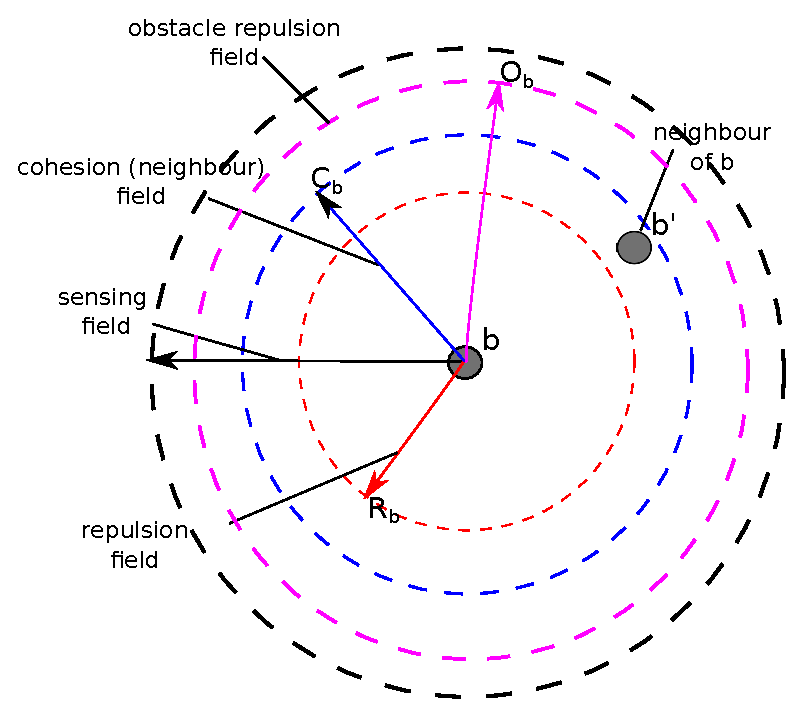
\includegraphics[width=7cm]{CHAPTER-2/figures/FieldEffects}
\end{center}
\caption{Agent field effects\label{methods:FieldEffects}}
\end{figure}

A swarm is modelled as a set of agents~\cite{MIN:07, VY:04}. An agent is modelled as a point in 2 dimensional space with no mass or size. This is similar to the representation used by Vankerkom and Yu to visualise swarms~\cite{VY:04}. Mohan and Ponnambalam, and Gazi and Passino~\cite{VY:04, GP:04}, Barnes et al.~\cite{BAF:06, BAFVM:06, BFV:07} and Bennet and McInnes~\cite{BM:09} and Andreou et al.~\cite{APZDAMC:09} also use a similar model which includes agents moving at a constant speed.

The interaction of agents within a swarm is modelled using vectorial and geometric techniques~\cite{HER:11, BAF:06}. The position of an agent is modelled using cartesian coordinates and the movements are modelled using vectors. The position vector is given by the coordinates of an agent.

The `world' that the swarm is modelled within is an unbounded 2 dimensional Euclidean plain.  

The use of vectors to model inter-agent interactions is also referred to a artificial potential fields~\cite{VG:05, XJYYH:10, SW:03, BAF:06, BAFVM:06, BFV:07, BM:09, HC:09} or vector fields~\cite{YH:14, GKF:13, PZ:13}. 
%% The mathematical techniques used to achieve the modelling are geometry and vector mathematics~\cite{HER:11, BAF:06}. The positional aspects of agents are modelled in the form of coordinate geometry and the movements are modelled using vector mathematics. These modelling techniques are highlighted in surveys carried out by Holmstr{\"o} and Romero~\cite{HR:ND}, Minor~\cite{MIN:07} and Muniganti and Pujol~\cite{MP:10}. 


%% Swarms can be modelled in two~\cite{MIN:07, VY:04} or three~\cite{BSB:15} dimensions.
%% This thesis uses a two dimensional model with unbounded ranges.%% \section{Swarming plane}
%% The modelling of swarms can be carried out in two dimensional planes. Swarms can be modelled in three dimensional space using the three axis of $x,y,z$~\cite{BSB:15} or two dimensional space using $x,y$~\cite{MIN:07, VY:04}.
%%  
%% This thesis uses a 2D Euclidean plane $(x,y)$. The dimensions of the plane are unlimited $(-\infty< x,y <+\infty)$ with a central origin of $(0,0)$. All the techniques discussed in this thesis could be transitioned to 3D space~\cite{PG:08} as a 2D environment can be considered as being a 3D environment with the $z$ axis set to $0$. 
                                
%% \section{Environment modelling principle}\label{method:RealNumberModelling}
%% Each agent's position within a swarm is modelled as a point consisting of two floating point numbers to represent their $(x,y)$ position.

\section{Modelling agents and environment interactions}\label{method:AgentEnvironmentModel}
The environment contains agents with a position in the coordinate system. It may also contain \textit{obstacles}~(Figure~\ref{section:ObstacleSection}) and \textit{destinations}~(Figure~\ref{sec:Direction1}). An obstacle can be considered as a point with an associated \textit{repulsion field} effect and a destination as a point towards which agents move. This modelling technique is similar to that used by Barnes et al.~\cite{BAF:06, BAFVM:06}. 
%% Modelling of the swarm will be performed using two techniques; vectors for inter-object interactions and coordinates for positional locations. The proximity of each of the objects within the swarm are identified, the objects being, agents, obstacles and destinations. The effects of the objects upon each other are determined using fixed ranges (field effects). 

The distribution of each of these objects, along with the field effects, produce sets of vectors that represent the inter-object interactions in the system. The vector sets for each agent are used to calculate a vector for each interaction type (cohesion, repulsion, direction, and obstacle repulsion). This is similar to the techniques used by Jung et al. and Salda\~na et al.~\cite{JG:13, SOM:12}. 

The resultant vector generated by an agent's interaction with other agents and obstacles is referred to as the agent's \textit{interaction vector}. The resultant vector generated between two agents is referred to as the \textit{inter-agent vector}. The vector applied to an agent to influence its movement towards a destination is referred to as the agent's \textit{destination vector}. The weighted combination of the \textit{destination vector} and the \textit{interaction vector} produces the \textit{movement-direction vector}. \textit{The movement-direction vector} indicates the direction an agent may move. 

%% \subsubsection{Swarming algorithms/model check} 
%% When calculating movement in a simulation the distance moved by the agents must be modelled in such a way that physically impossible scenarios do not occur. As agents are simulated mathematically it is possible for the simulation to calculate a path that would allow two agents to pass through the same space ($x,y$) at the same time. It is also possible to create environmental configurations that would allow an inter-object effect to be missed. This can be caused by the model not identifying agents passing through a field effect due to its calculated movement extending beyond or crossing a field effect in one time increment. 
%% These potential situations are eliminated by ensuring the sampling rate is a multiple of the clock cycle for calculating field effects, and the movement of an agent is less than any of the field effects. This check is incorporated into the simulator as a parameter check when the physics model of the graphical simulator is changed.

\section{Boid-based model}\label{methods:BoidModel}
The model introduced in~Figure~\ref{method:AgentEnvironmentModel} is based heavily on the work by Reynolds and other authors on boid-based swarms.

Hereford~\cite{HER:11} and Barnes et al.~\cite{BAF:06} model static swarms using a bi-variable technique. A bi-variable model is based upon inter-agent cohesion and repulsion, which appears as the \textit{interaction vector} above. 

Gazi and Passino also used this bi-variable technique to examine inter-agent interactions when creating stable swarm structures and ensuring agents remain part of a swarm while not colliding~\cite{GP:04a, GP:02, GP:04}. They define the degree to which an agent remains cohesive to a swarm as an agent's stability. 

If a swarm is to be goal based, the swarm is modelled using the \textit{interaction vector} and a \textit{destination vector} to create the \textit{movement-direction vector} as discussed by Salda\~na et al., Stranders et al., Nash and Koenig~\cite{SOM:12, SRDF:10, NK:10}. 

The first swarming model to use three components was the Boid model~\cite{REY:87}. In the Boid model, cohesion and repulsion are used to produce an \textit{inter-agent vector}. The main difference in the model is how the \textit{destination vector} is introduced. In a Boid swarm the \textit{destination vector} is not based upon a fixed destination. It is determined by each agent communicating with its neighbours to generate a consensus-based direction. Each agent calculates an average of the neighbours \textit{movement-direction vector} and applies the result as a \textit{destination vector}. This consensus-based movement creates a `flocking' effect~\cite{KC:08, REY:87}. This cooperative method of creating movement can be seen in the formation of fish shoals as discussed by Yang et al.~\cite{YGT:10} and Pearce et al.~\cite{PMRT:14}. The same flocking characteristic also occurs in starling murmurations as discussed by Campbell and Samsel~\cite{CS:15}, and Zhang et al.~\cite{ZZLW:14}. 

Barnes et al., Bennet and McInnes, Cai et al. Correl and Rus, Dinolov et al. and Ekanayake and Pathirana take a different approach to creating a \textit{destination vector}~\cite{BAF:06, BAFVM:06, BM:09, CML:ND, CR:13, DLK:11, EP:10}. They generate a \textit{destination vector} in a similar manner to that described in Figure~\ref{method:AgentEnvironmentModel} using the \textit{interaction vector} and the \textit{destination vector}.
%% The agent's position can be determined by using a sensor such as a GPS. The directional vector is added to the interaction vector. Adding the directional bias and the interaction vector produces a goal based characteristic in the resultant movement vector.
%% 
%% This thesis will use a similar method of generating a directional vector from a fixed destination to produce a \textit{Boid-based} directional model.  

\section{Swarm cohesion}\label{sec:Cohesion1}
Several views of cohesion exist within the swarm research community. Cohesion, in some cases, is considered as an agent moving towards the centroid of a swarm. The centroid is the centre of the swarm. This approach is used by Gazi and Passino who measure stability based on changes in distance from the centroid of a swarm~\cite{GP:11, GP:04}. They define stability as the `degree' to which a swarm will remain a coherent entity. Shinichi et al.~\cite{AYSH:08} also use the concept of the centroid of a swarm to define a metric to measure stability.

Alternatively Long et al.~\cite{QZYP:13}, Shinichi et al.~\cite{AYSH:08} and Ekanayake and Pathirana~\cite{EP:10} refer to cohesion as an `attractive force' and define cohesion as being localised to an agent and its `visible' neighbours. The visibility they discuss is determined by a sensor that provides localised proximity information that includes angles and distances to neighbouring agents.
 
Similarly, this thesis will view cohesion as the interaction of an agent with its local neighbours. Agents are viewed as being autonomous using only localised proximity information. The Boid model requires information about the swarm's structure, the positions and directions of neighbours. This requires a communications infrastructure. The model in this thesis does not require this information and therefore does not require a communications infrastructure.

This thesis, when analysing the data captured from an experiment, will only use the centroid as a means of tracking the position of a swarm. The centroid and the logic to identify it will not be used by agent algorithms for coordination. 

Cohesion is based on the principle that all agents will remain part of their immediate neighbours' `cluster' and will `flock' together in a `localised' manner~\cite{VGHHDM:15, BAF:06, BAFVM:06, BFV:07, BM:09, HAY:08, HCS:09}. Localised being that the agents will only be `aware' of their immediate neighbours. 

Flocking, in this thesis, should be considered as the process of agents moving towards each other to attain their most stable position~\cite{GMJ:11, IGMFM:08} which is the centre of mass of their immediate neighbours~(Figure~\ref{methods:FlyToCentre1}). 

The cohesion vector is calculated by summing the relative position vectors identified from the origin agent ($b$) to each neighbouring agent. This vector is divided by the total number of neighbour agents~(Figure~\ref{eq:FlyToCentre1}) to produce a resultant cohesion vector. The closer a neighbouring agent is to the agent of interest then the smaller the cohesion vector generated.

\begin{figure}[H]
\begin{center}
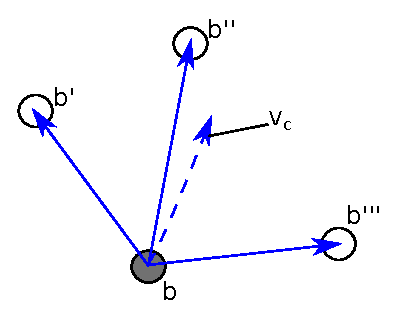
\includegraphics[width=5cm]{CHAPTER-2/figures/FlyToCentre1}
\end{center}
\caption{Cohesion: Origin $b$ \label{methods:FlyToCentre1}}
\end{figure}

Formally the cohesion vector $v_{c}(b)$ for agent $b$ is the vector calculated by summing the vectors $bb'$ formed from the agent to each of its neighbours~$b' \in nbr(b)$~\cite{HAY:08} and dividing by the number of neighbours.

%% $S$ is a swarm of size $N$ represented as a set of $N$ agents.
%% 
%% \begin{equation}\label{eq:Swarm1}
%% S \buildrel \Delta \over = \{b_{1}\ldots b_{N}\}
%% \end{equation}‎

A neighbour of $b$ is any agent within the swarm $S$ that is within neighbour range:

\begin{equation}\label{eq:Neighbours1}
nbr(b) \buildrel \Delta \over = \{b' \in S~:~\magn{bb'} <= C_b\}
\end{equation}‎

\begin{equation}\label{eq:FlyToCentre1}
v_{c}(b) = \frac{\mathlarger{\sum_{b' \in nbr(b)}}{bb'}}{\card{nbr(b)}}
\end{equation}‎

\section{Swarm repulsion}\label{sec:Repulsion1}
Repulsion is defined by Reynolds, Kawabayashi and Chen, and Shinichi et al. as the tendency for an agent to move away from another agent that enters its repulsion field~\cite{REY:87, KC:08, AYSH:08}. This creates a `field effect' around the agent such that when another agent enters that area a vector is applied to prevent the agents colliding. Repulsion is also applied to agents when they interact with obstacles, this is covered in~Figure~\ref{section:ObstacleSection}.

Kawabayashi and Chen~\cite{KC:08}, Reynolds~\cite{REY:87} and Aso et al. implement repulsion as a vector at a boundary with a fixed magnitude~(Figure~\ref{methods:Repulsion3}). 

\begin{figure}[H]
\begin{center}
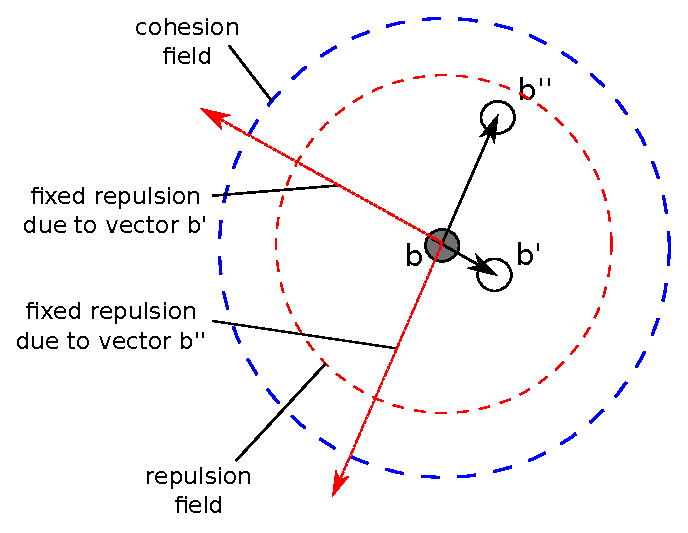
\includegraphics[width=7cm]{CHAPTER-2/figures/Repulsion3}
\caption{Agent fixed magnitude repulsion\label{methods:Repulsion3}}
\end{center}
\end{figure}

This approach produces a resultant repulsion vector that is based upon the angles at which the neighbour agents approach an agent without considering the proximity of the neighbours to the agent. 

In this thesis the repulsion vector has a graduated magnitude. Each neighbouring agent's repulsive effect is applied proportionally~(Figure~\ref{methods:Repulsion1}). When an agent encroaches upon another agent the degree of the field intrusion is mapped to a value in the range $0 \rightarrow 1$. This affects the magnitude of the repulsive vectors that are applied and therefore the resultant repulsion vector~(Figure~\ref{methods:Repulsion4}). 

\begin{figure}[H]
\begin{center}
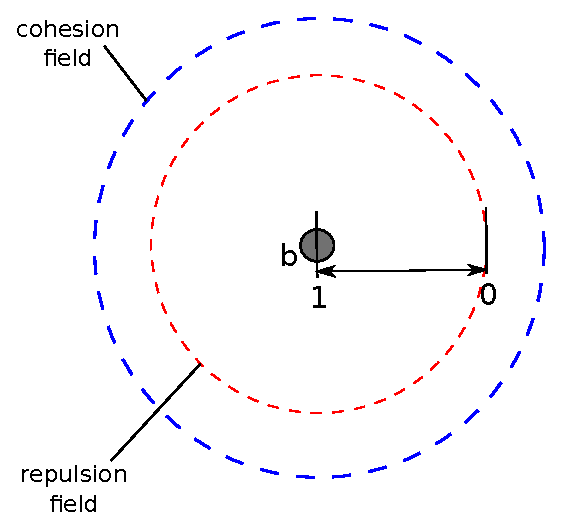
\includegraphics[width=8cm]{CHAPTER-2/figures/Repulsion1}
\caption{Graduated agent repulsion \label{methods:Repulsion1}}
\end{center}
\end{figure}

This technique changes the repulsion vector such that the direction reduces the probability of a collision. In this thesis the inter-agent repulsion will be calculated as the average of all the proportional repulsion vectors~(Figure~\ref{methods:Repulsion2}). 
 
\begin{figure}[H]
\begin{center}
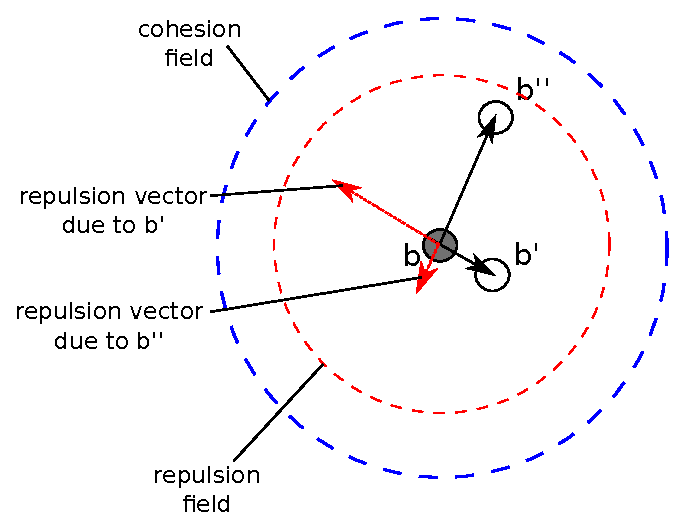
\includegraphics[width=7.5cm]{CHAPTER-2/figures/Repulsion2}
\caption{Proportional agent repulsion \label{methods:Repulsion2}}
\end{center}
\end{figure}

Figure~\ref{methods:Repulsion4} shows a comparison of the two repulsion models with the proportional repulsion magnitude shown in green and the fixed magnitude shown in red. The two models produce different repulsion angles. The angle produced by the proportional model increases the distance agent ($b$) will move away from $b'$ when motion is applied. This reduces the chance of a collision between the two agents. The proposed proportional model is therefore suited to swarm's where agent collisions may cause problems. 

\begin{figure}[H]
\begin{center}
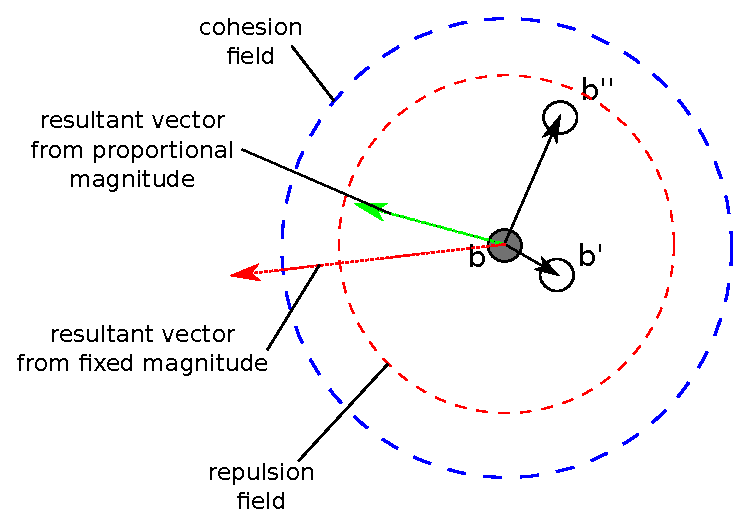
\includegraphics[width=8cm]{CHAPTER-2/figures/Repulsion4}
\caption{Repulsion comparison\label{methods:Repulsion4}}
\end{center}
\end{figure}

To calculate the total inter-agent repulsion the neighbours that are within the repulsion field must be identified. This is shown in~Figure~\ref{eq:Repulsion2}.

$R(b)$ is the set of all agents that are within the repulsion field. $R_b$ is the repulsion field and $\magn{bb'}$ is the distance between~$b$ and its neighbour~$b'$.  

\begin{equation}
\label{eq:Repulsion2}
R(b) = \{b' \in S~:~\magn{bb'} <= R_b\}
\end{equation}

$v_{r}(b)$ is the repulsion vector generated for agent $b$ based on the proximity of its neighbours. If $R(b)$ is empty then $v_{r}(b) = 0$ otherwise it is given by~equation~\ref{eq:Repulsion1}. The proportion of field intrusion is calculated by $1-\frac{\magn{bb'}}{R_b}$. The field effect distance $R_b$ is the range around the agent where the repulsion effect is introduced to prevent collisions. 

\begin{equation}
\label{eq:Repulsion1}
v_{r}(b) =‎ -
\frac{1}{\card{R(b)}}
\left(
\mathlarger{\mathlarger{\sum_{b' \in R(b)}}}
{\left( 1-\frac{\magn{bb'}}{R_b} \right)}
{bb'}
\right)
\end{equation}‎

\section{Swarm agents/obstacles interactions\label{section:ObstacleSection}}
Obstacles, like agents, can be represented as a point in the system. As an agent moves it may enter an obstacle's \textit{obstacle repulsion field} causing the agent to move away.

In this thesis agents are modelled with a fixed obstacle repulsion distance $O_b$ where a repulsion vector is applied. The repulsion is then a vector of magnitude $O_b$. If more than one obstacle is within the field effect agent the total repulsion vector is the sum of the repulsion vectors due to each obstacle~Figure~\ref{methods:Obstacle1}. The result is normalised and scaled such that the magnitude is the same as the field distance~$O_b$.

\begin{figure}[H]
\begin{center}
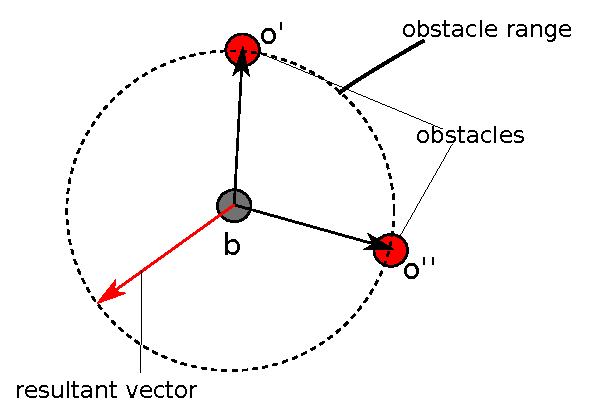
\includegraphics[width=6cm]{CHAPTER-2/figures/Obstacle1}
\end{center}
\caption{Obstacle repulsion \label{methods:Obstacle1}}
\end{figure}

%% $O$ is a set of $N$ obstacles.
%% 
%% \begin{center} \label{eq:Obstacle1}
%% \begin{equation}‎
%% O \buildrel \Delta \over =‎ \{o_1\ldots o_N\}
%% \end{equation}‎
%% \end{center}

%% $o' \in O:|bo'| < O_b$ the set of obstacles that are within range of agent $b$, where $O$ is the set of obstacles. 

%% \begin{center} \label{eq:Obstacle4}
%% \begin{equation}‎
%% R(b) \buildrel \Delta \over =‎ \{o' \in O:|bo'| < O_b\}
%% \end{equation}‎
%% \end{center}

Equation~\ref{eq:Obstacle2} shows the resultant repulsion vector $v_o(b)$ for an agent. $\{o~\in~O~:~\magn{bo}~<=~O_b\}$ is the set of obstacles that are within range of agent $b$. $O$ is the set of obstacles. The obstacles are identified using the distance between an agent and an obstacle $\magn{bo}$ and comparing the result to the fixed obstacle repulsion range~$O_b$. The result is calculated by scaling the normalised sum of the normalised vectors $(ob)\string^$ by $O_b$. Note that \string^ is the equivalent of $\hat{v} = \frac{v}{\magn{v}}$ the normalised vector.

\begin{center} 
\begin{equation}\label{eq:Obstacle2}‎
v_o(b) =‎ O_b\Bigg(\mathlarger{\mathlarger{\mathlarger{\sum}}}_{o \in O~:~\magn{ob} <= O_b}(ob)\string^\Bigg)\string^
\end{equation}‎
\end{center}

%% \begin{center} \label{eq:Obstacle3}
%% \begin{equation}‎
%% v_o(b) =‎ |l_o(b)|O_b
%% \end{equation}‎
%% \end{center}

\section{Swarm direction (goal based swarms)}\label{sec:Direction1}
There are two directional aspects to swarm motion. The \textit{interaction vector} which is the vector created by inter-agent reactions through the cohesive and repulsive fields as discussed in~Figure~\ref{sec:Cohesion1} and~Figure~\ref{sec:Repulsion1} and the vector for avoidance of obstacles~Figure~\ref{section:ObstacleSection}. The \textit{destination vector} is applied to influence the motion of a agent towards a particular coordinate~\cite{BHK:07} and the \textit{interaction vector} to maintain the swarm's structure. This model is used by Barnes et al.~\cite{BAF:06, BAFVM:06}, Bennet and McInnes~\cite{BM:09}, Cai et al.~\cite{CML:ND}, Correll and Rus~\cite{CR:13}, Dinolov et al.~\cite{DLK:11} and Ekanayake et al.~\cite{EP:10}. This thesis uses a similar technique, defining a single destination as a \textit{destination vector} for goal based swarms. The application and effect of multiple destinations is discussed in future work. 

%% \begin{figure}[H]
%% \begin{center}
%% \includegraphics[width=7cm]{CHAPTER-2/figures/Destination1}
%% \caption{Destination vector\label{methods:Destination1}}
%% \end{center}
%% \end{figure}

$v_d(b)$~(Equation~\ref{eq:Destination1}) is the \textit{destination vector} where $d$ is the destination. 

\begin{center}
\begin{equation}\label{eq:Destination1}‎
v_{d}(b) =‎ bd
\end{equation}‎
\end{center}

\section{Weighted movement-direction model}\label{methods:weightedModel}
An agent's \textit{movement-destination vector} is the sum of all the component vectors ($v_c, v_r, v_d, v_o$) (Equation~\ref{eq:BotDirection1})~\cite{HAY:08}. For a vector to be used for movement it must have a magnitude of 1 before the agent's speed can be applied (Section~\ref{sec:Direction1}).

%%  as shown in~(\autoref{eq:BotDirection1}).
 
\begin{center}
\begin{equation}
\label{eq:BotDirection1}
v(b) =‎ v_{c}(b) + v_{r}(b) + v_{d}(b) + v_{o}(b)
\end{equation}‎
\end{center}

%% Note: \string^ is the equivalent of $\hat{v} = \frac{v}{|v|}$ the normalised vector.

This model is extended by adding a weighting to each of the component vectors. The addition of the weightings allows the influence of each component vector set to be adjusted to produce a bespoke movement vector~(\autoref{methods:weightedModel}). The resultant vector is normalised to produce a unit \textit{movement-direction vector} that can be used to create motion~\cite{KC:08}. The agent's speed characteristic is used along with time~($t$)~\cite{FAP:05, GP:05} to determine an agent's next position. This derived vector is the \textit{movement vector}.

The purpose of a weighted aggregation model is to alter the level of influence of each component of the equation. This technique is generally referred to as a \textit{`weighted sum aggregation'} or \textit{`ordered weighted averaging'}. The technique is applied to optimisation algorithms such as PSO (Particle Swarm Optimisation) and involves applying all the possible combinations of weightings to a multi-variable expression to obtain an optimum output~\cite{MV:12, XTH:09}.

In this thesis the technique of \textit{weighted sum aggregation} is applied to the vector calculations to allow tuning of the swarming algorithm of an agent and to change the degree of influence to obtain a required swarming effect. 

The tuning is applied to each component as a weighing factor $k$~Equation~\ref{eq:BotPhysics1}. The weightings ($k_c, k_r, k_d, k_o$) are applied before normalising the \textit{movement-directional vector}. This change of bias allows levels of importance to be applied to a system characteristic i.e. $k_c > k_d$ implies it is more important for the agents to remain together than it is to travel towards the destination. This technique is similar to those identified by Muniganti and Pujol in their survey of mathematical modelling techniques~\cite{MP:10}. 

Weightings can be applied in several ways. The weighting can be applied as a set of arbitrary integer values (12, 67, 99) or as a set of values that always have a summed value of 1 e.g. 0.5, 0.25, 0.25. Either of these techniques are acceptable as the resultant vector is normalised following the application of the weighting. This thesis implements the weightings as a set of arbitrary integer values~(Equation~\ref{eq:BotPhysics1}). Where $k_c$ is the weighting factor for cohesion, $k_r$ is the weighting factor for repulsion, $k_o$ is the weighting factor for obstacles and $k_d$ is the weighting factor for a destination. 

\begin{equation}\label{eq:BotPhysics1}‎
v(b) =‎ k_cv_c(b) + k_rv_r(b) + k_ov_o(b) + k_dv_d(b)
\end{equation}‎

Special cases of~Equation~\ref{eq:BotPhysics1} can be applied to a swarm model. A swarm with no destination can be modelled with the destination weighting set to zero to create the model shown in~Equation~\ref{eq:BotDirection2} as used in Chapter~\ref{chapter:flooding}. This is also known as the \textit{interaction vector}

\begin{center}
\begin{equation}
\label{eq:BotDirection2}
v(b) =‎ k_cv_c(b) + k_rv_r(b) + k_ov_o(b)
\end{equation}‎
\end{center}

A swarm that does not interact with obstacles and has no goal (destination) can have $k_o$ and $k_d$ set to zero creating the model as shown in~Equation~\ref{eq:BotDirection3}. This is also known as the \textit{inter-agent vector} as discussed in~\autoref{Section:StabilityModel} on page \pageref{Section:StabilityModel}.

\begin{center}
\begin{equation}
\label{eq:BotDirection3}
v(b) =‎ k_cv_c(b) + k_rv_r(b)
\end{equation}‎
\end{center}

Equation~\ref{eq:BotDirection3} is also the model used in the calculation of the swarm magnitude metric as discussed in chapter~\ref{chapter:metric} where $v(b) \equiv P(b)$.

\section{Modelling movement}\label{sec:Movement1}
Each agent within a swarm calculates its \textit{movement-direction vector} based on its \textit{interaction} and \textit{destination} vectors. The \textit{movement vector}~($b_{pos}$) is calculated using the unit \textit{movement-direction vector} of Equation~\ref{eq:BotPhysics1} multiplied by the time elapsed~($t$) in the system and the speed characteristic of the agent~($s_b$).

This process is carried out for every agent in the swarm to create the entire swarm's next position.

\begin{center}
\begin{equation}
\label{eq:AgentMovement}
b_{pos}=s_{b}t\big(v(b)\big)\string^ 
\end{equation}‎
\end{center}

The increment in the location of agent $b$ over time interval $t$ is shown in Equation~\ref{eq:AgentMovement} where $s_b$ is the speed of agent~$b$. Models of time are discussed in \autoref{chapter:simulator}. 

%% \begin{center}
%% \begin{equation}
%% \label{eq:BotSwarm2}
%% l(b) =‎ s_{b}t\big(v(b)\big)\string^
%% \end{equation}‎
%% \end{center}



%% \section{Swarming algorithms} 
%% The logic that produces the cooperative appearance of agents in a swarm are the algorithms that each agent applies to calculating their movement~\cite{BS:13, DLK:11, HAY:08}. There are many variation in how algorithms apply their effects~\cite{BBBV:04, DT:03}. The basis of all algorithms is that they consider two influencing factors, direction and speed~\cite{BAF:06, BAFVM:06, BVD:14, EP:10}. 
%% 
%% The application of the movement is therefore calculated using the time, speed and direction in discrete intervals as shown in~\autoref{method:SwarmParticipant} where $s_b$ is the agent speed, $t$ is time, $b$ is the agent and $v$ is the resultant vector that is used to calculate the movement.
%% 
%% \begin{figure}[H]
%% \begin{center}
%% \includegraphics[width=7cm]{CHAPTER-2/figures/SwarmParticipant}
%% \caption{Algorithm effects \label{method:SwarmParticipant}}
%% \end{center}
%% \end{figure}

\section{Stable swarm structures}
A swarming behaviour can be created using only cohesion and repulsion. This technique is known as a bi-variable model~\cite{BAF:06,BAFVM:06}. The bi-variable model produces natural geometric structures. The structures tend to be based on equilateral triangles and when the distribution of the agents allows, regular hexagons are formed. These structures only occur when the repulsion and cohesion field effects produce a distribution such that an agent's detected neighbours do not extend beyond the first agent detected in any direction~\cite{PCL:08, PCL:08a}. The effect of field effect ranges on a swarm's structure is discussed in chapter~\ref{chapter:SwarmType}.  

The most stable state for agents is for all agents to be equidistant with equal angles. If two agents are in close proximity they will naturally adhere to each other due to the proximity rule (cohesion)~(Figure~\ref{fig:StableForms}); repulsion will ensure a minimum distance is preserved. In the case of 3 agents a triangle will form. In the case of 4 agents the most stable shape will be a diamond with the centre agents joined. With 5 and 6 agents a triangular lattice will emerge and with 7 agents a stable hexagon will form. The hexagon~(Figure~\ref{fig:StableFormHexagon}) is the most stable structure with all agents being equidistant and all angles between each neighbouring agent equal~\cite{BAF:06, GP:05}. These structures are seen throughout the natural world~\cite{RAZ:13}.

\begin{figure}[H]
\begin{center}
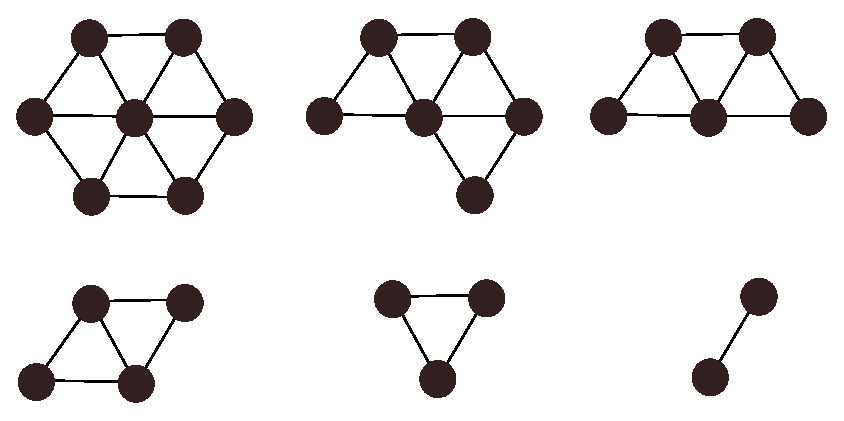
\includegraphics[width=7cm]{CHAPTER-2/figures/StableForms}
\end{center}
\caption{Stable swarm formations}\label{fig:StableForms}
\end{figure}

\begin{figure}[H]
\begin{center}
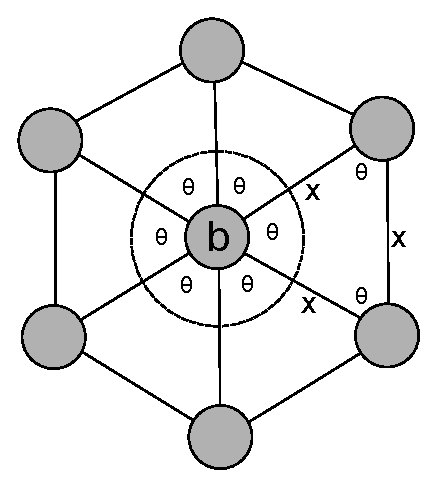
\includegraphics[width=4cm]{CHAPTER-2/figures/Hexagon}
\end{center}
\caption{Stable hexagonal formation}\label{fig:StableFormHexagon}
\end{figure}



\section{Resultant swarm model}
The swarm model created by~Equation~\ref{eq:BotPhysics1} with suitable weightings will allow a swarm to form `stable' structures such that the agents will remain connected~(\autoref{methods:Stable1}) and over time migrate to an optimum overall structure for the models parameters. The parameters are the field effect ranges, the cohesion and repulsion magnitude models and the weightings. 

The initial random deployment of a set of agents to create a swarm produces a `disorganised' state. The disorganisation is caused by the varying cohesion and repulsion vectors that are generated by the inter-agent relationships. Following the initial deployment the magnitudes will create movements that gradually stabilise the swarm structure to a level of movement that best fits the model parameters~\cite{PG:08, WF:12}. The point of equilibrium for the swarm and the resultant structure is dependent upon the agent's cohesion and repulsion fields level of overlapping. This is discussed in \autoref{section:AnalysisA} and~\autoref{section:AnalysisB}.

When modelling swarms it is common practice to have the agents in constant motion~\cite{LCW:07, GKF:13}. In this thesis agents are modelled moving at a constant speed with no inertial effect such that an agent can move freely within the system plane. The only exception to this will be if an equilibrium state is encountered where the summed vectors produce a null vector. If this occurs the agent will stop moving.

\section{Swarm deployment}

Using the methods discussed in this chapter, a swarming behaviour emerges from
a collection of agents. The initial deployment of a swarm may be a random
dispersal of agents such that the swarm is in a disorganised
state~(\ref{methods:Chaos1}), caused by an instability in the magnitudes that
are acting upon each of the agents (as detailed above). Based upon the
application of the models discussed, the swarm will initially move in such a
way as to balance all the vectors, resulting in a period of disorganisation
where the swarm's movement towards a goal is limited, as the vectors generated
to disperse the agents outweigh the directional vector. 

This phase of the swarm's life cycle is the `initialisation
phase'~(Figure~\ref{methods:StableTime1}). When the initialisation phase is
over, the vectors (cohesion, repulsion, and direction) become more balanced and
the swarm forms a more regular shape, such as a hexagonal lattice, where all
the angles and lengths (distances between agents) tend toward being
equal~(Figure~\ref{methods:Stable1})

The effects can be seem in the screenshots (Figures \ref{methods:Chaos1},
\ref{methods:Stable1}, \ref{methods:StableTime1}) from the simulator discussed
in~\autoref{chapter:simulator}.

\begin{figure}[H]
\begin{center}
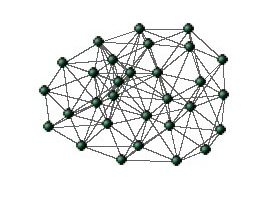
\includegraphics[width=7cm]{CHAPTER-2/figures/Chaos}
\end{center}
\caption{Disorganised swarm\label{methods:Chaos1}}
\end{figure}

\begin{figure}[H]
\begin{center}
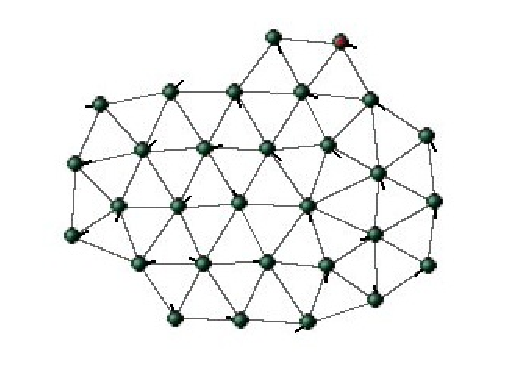
\includegraphics[width=7cm]{CHAPTER-2/figures/Stable}
\end{center}
\caption{Stable swarm\label{methods:Stable1}}
\end{figure}

\begin{figure}[H]
\begin{center}
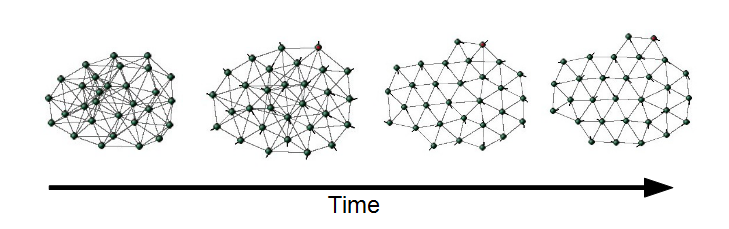
\includegraphics[width=10cm]{CHAPTER-2/figures/StableTime}
\end{center}
\caption{Swarm stabilisation\label{methods:StableTime1}}
\end{figure}

\section{Swarm simulator}\label{chapter:simulator}
Swarm behaviours can be investigated by means of experiments with physical robots or by means of simulations. The latter approach has the advantages of scalability, generalisation, speed of development, and cost. This thesis is based upon data generated from simulated swarms. There are several open source robotic simulators available, the most popular being ARGoS, Player/Stage, and Gazebo.

ARGoS is described as a multi-physics simulator and has gained interest in the swarm robots community. In 2011 Luca and Caro published an overview of the simulator's engine discussing how the system functioned~\cite{PTOPB:11} and the philosophy behind its structure. They also published a framework for using the simulator in 2012~\cite{KCGD:12}. 

Player/Stage and Player/Gazebo are used in many projects including projects simulating single robots as discussed by Song and Gupta~\cite{SG:15} and also multiple-robot swarming simulations as described by Lei et al~\cite{LLZ:08}. There are projects that have simulated the use of pheromone trails when simulating foraging based swarms as discussed by Shi et al~\cite{STZZW:13}. Shi et al. have also published an overview of the scenarios in which Player/Stage can be used~\cite{STWZZ:11}.

The Webot~\cite{CL:16} simulator, which is a commercial product, has been used successfully in other research projects such as the swarm simulations developed by Srivastava and Nandi~\cite{SN:10}. One problem found with the product was that it was restrictive in terms of how much of the system could be configured to meet the needs of the thesis. Another factor that had to be taken into consideration was the high cost of a licence for the PRO version of Webot.

These simulators all provide a discrete time simulation environment. The main purpose of these simulators is to visualise either an individual robot or a swarm of robots based on a model that is defined through bespoke libraries and configuration parameters. On the other hand, in this thesis the main purpose of each simulation is to log all the positional and vector data associated with every agent at each discrete time interval. Due to this disparity in approaches it was decided to develop a simulator whose main purpose is the collection of data on distance, positions, distribution and inter-object vector magnitude influence. 

This section discusses the design, development and usage of the simulator used in this thesis and the creation of the raw experimental data. The section also discusses how the data is processed to produce the aggregated data required for visualisation.

%\section{Introduction}\label{sim:intro}

\subsection{Simulator overview}\label{sim:intro}
The simulator has two distinct components: a graphical design/simulation tool~(Appendix~\ref{AP2:GRAPH}) and a command line based simulation-only tool~(Appendix~\ref{AP2:CLI}). Both parts of the simulator are written in Python 3~\cite{PYTHON3:15} using an object model as shown in~appendix~\ref{app5}. Both use the same modelling engine by sharing the base classes.  The final object model is similar to that proposed by Vankerkom and Yu for swarm visualisation~\cite{VY:04}. The simulator design is also influenced by the \textit{`main loop'} proposed in the ARGoS simulator~\cite{PTOPB:11}.

\subsection{Simulator architecture}\label{sim:Simulator2}
The main purpose of the graphical environment is for the setup of an experiment's initial configuration. This is achieved by positioning the agents, destinations, and obstacles in an environment and saving the configuration as a simulation file. As a secondary purpose the graphical environment is capable of running small scale simulations. The command line tool is used to execute the simulation experiments designed using the graphical tool. 

The graphical tool, shown as (1) in~Figure~\ref{sim:SimulatorOverview}, uses PyGame~\cite{PYGAME:15} as its graphical presentation layer. PyGame supports several rendering engines; in this application the default SDL rendering engine is used. The graphical simulator runs in real-time and is capable of simulating small swarms of \textless~150 agents on a PC with an \texttt{Intel® Core™ i7-4770 CPU @ 3.40GHz * 8} processor. This swarm size limitation is due to the Python code being executed on a single processor core. There is also a limitation in the performance of the graphical engine due to the rendering being performed by the interpreter.
 
The command line tool, shown as (2) in~Figure~\ref{sim:SimulatorOverview}, reads in the experiment configuration file generated via the graphical tool, shown as (1). The command line tool uses simulated discrete time~(Figure~\ref{sim:time}) and is able to run with arbitrary sized swarms without real-time processing limitations. The command line tool simulates the swarm and generates the initial data extract (3a). The data extract is then loaded into a MySQL database (3b) and the data is then aggregated to create the complete dataset for the experiment (4). The processes 5 and 6 are discussed in~Figure~\ref{sim:GraphingTools}.  This thesis deals with arbitrary sized swarms, so simulations are designed in the graphical environment but executed using the command-line-based simulator. 

\begin{figure}[H]
\begin{center}
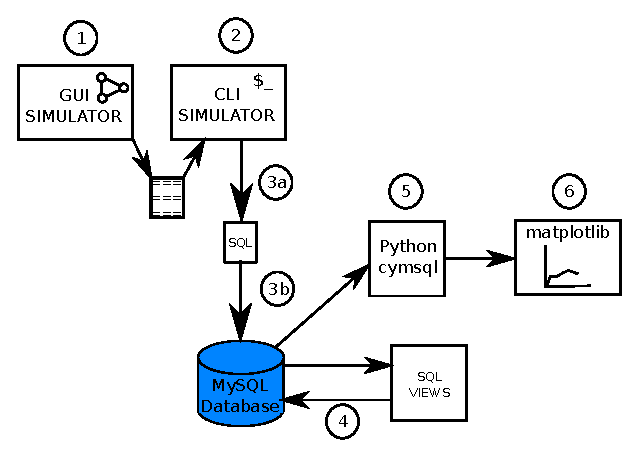
\includegraphics[width=10cm]{CHAPTER-3/figures/SimulatorProcess}
\end{center}
\caption{Simulator process overview\label{sim:SimulatorOverview}}
\end{figure}

Figure~\ref{sim:SimulatorOverview} shows the stages of the simulation from developing an experiment~(1) through to the production of simulation results~(6).

\subsection{Simulated time}\label{sim:time}
There are two options for representing time when modelling a swarm: continuous
time and discrete time. Continuous time~\cite{HW:08} is \textit{dense}: between
any two points in time there is another point. Discrete time~\cite{FAP:05,
GP:05, RVMH:13, HER:11, MP:10, PCL:08a} on the other hand proceeds in `ticks'
with no intermediate time points. In this thesis discrete time is used. This
same approach is identified by Muniganti and Pujol in their survey of
mathematical swarming models~\cite{MP:10}. 

Vision based coordination for robots was a subject of great interest in the
1980s and 90s~\cite{DK:02}. This interest moved to omni-directional cameras as
a means of determine position and mapping through image analysis in a process
known as SLAM (Simultaneous Localisation And Mapping)~\cite{TRI:15,SG:15}. A
general purpose omni-directional camera can operate at speeds between 1Hz and
60Hz, depending upon the resolution of the images and the accuracy of the
positional data required. 

For the identification of an agent's position, a GPS with a sample rate in the
same range may be used. For example, the SparkFun Venus GPS~\cite{SF:16}
operates at up to 20Hz.

The simulator allows the sampling rate to be adjusted to provide a model that
is as close as possible to the physical sensors. For the experiments in this
thesis, the sample rate is set at 10Hz, clearly within the scope of currently 
available sensors. This gives a `tick' interval of 100ms.

\subsection{Simulated field effects}
The ranges for the cohesion, repulsion, and obstacle avoidance fields are user-configurable
parameters in the simulator, as is the location of a destination goal, if present.
The simulation of the operations of cohesion, repulsion, obstacle avoidance and goal-seeking 
then directly follow the definitions given by equations~\ref{eq:FlyToCentre1}, \ref{eq:Repulsion1},
\ref{eq:Obstacle2}, and \ref{eq:Destination1}. The details of 
the implementation are shown in Appendix~\ref{sim:PythonCode}.

\subsection{Simulated agent movement}
The motion model of the simulation is implemented through the modelling of
vectors that influence an agent's resultant direction. The vectors that model
the swarm environment are the cohesion and repulsion vectors created by
inter-agent and inter-object interactions. 

Agent positions are modelled using floating point numbers. These coordinates
are translated to integer based $(x,y)$ co-ordinates for the presentation
layer. The integer translation is only for the visualisation of the swarm. This
is the same approach used by Vankerkom and Yu in their paper on swarm
visualisation~\cite{VY:04}. They model the agent using a class that consists of
positional variables of type double. This is also seen in the SwarmVis software
developed by Miner and Kasch~\cite{DMNK:ND}.

The incremental positions of the agents are calculated based upon the simulated time
slice, `tick', as discussed in~\autoref{sim:time}, and the agent speed, given as
a parameter of the simulation. These parameters are used as $t$ and $s_b$, respectively,
in applying Equation~\ref{eq:AgentMovement} to the calculation of the position of 
each agent at the next 'tick'. This movement is implemented within the simulator
as shown in Appendix~\ref{sim:AgentModelImplementation}.

\subsection{Simulator data capture}
To enable the analysis of a simulation run, the simulator generates an SQL database. 
As a simulation executes, at each tick, the state of each agent in the
swarm is captured and the data is saved as a pair of SQL insertions, 
$(\mathit{tick\ number}, \mathit{agents'\ states})$, that are
added to a set of transaction files. The implementation of the data capture
component of the simulator is described in detail in~Appendix~\ref{sim:DataAnalysis}.
This approach generates a large amount of data but allows for very detailed, offline
analysis of swarm behaviour.

\section{Conclusion}
This chapter notes the trend in using vectors as a modelling technique for
swarms and discusses the use of field effects in determining agent movement.
The chapter then introduces the mathematical model that is applied throughout
the thesis. The introduction covers the cohesion model that ensures agents
remain part of a swarm and the repulsion model that ensures agents do not
collide with each other, thus maintaining a stable swarm structure. The
chapter also introduces two additional aspects of swarming to the model:
goal-based direction and obstacle avoidance.  Finally, the chapter discusses
the simulation of swarms.  All simulations in this thesis are carried out using
the simulator described in this chapter. The data created by each simulation is
aggregated to generate the final datasets that allow the characteristics of the
simulated swarm to be evaluated. Data analysis results are visualised from the
aggregated data. 

  %general methods.
%\chapter{Summary and additional work}\label{Future}
\section{Summary of contributions}
In chapter~\ref{introduction} this thesis explores the basic constructs of how animals interact in different types of swarms such as shoals of fish, murmurations of starlings, and ant colonies. The chapter examines how these biological swarms have been studied and modelled to produced autonomous multi-agent robotic systems. The evolution of swarming techniques from the early modelling and mimicking of the biological swarms has shown that metrics are needed to provide an understanding of how agent interactions change over time and how the swarming algorithms affect the resultant swarm structures.

The remainder of the section focuses on the major contributions of the research:

\begin{itemize}
\item Model/Simulator
\item Inter-agent magnitude metric/Swarm Types
\item Perimeter coordination
\item Concave Reduction
\item Flood filling
\end{itemize}

\subsection{Model/Simulator}

Earlier research has identified the use of field effects as being an effective
method of modelling an agent's behaviour within a swarm. This has led to vector
mathematics being the most prominent mathematical modelling tool in swarm
theory. Field effect modelling through vector mathematics is discussed in
chapter~\ref{chapter:methods}. This chapter also introduces a graduated field
effect implementation for cohesion~(\autoref{sec:Cohesion1}) and
repulsion~(\autoref{sec:Repulsion1}) this approach helps to reduce collisions.
The model also applies an aggregate weighted model that allows the field effect
algorithms to be tailored to create regular
structures~(\autoref{methods:weightedModel}).

All of the experimental work in this thesis has been carried out using a
simulator written specifically for this project.
Section~\ref{chapter:simulator} discusses the simulation process and the object
model used for the representation of the swarming agents. The section discusses
the mathematical models that have been applied to the simulation. The section
also discusses how the simulator is applied to the experiments and how the
results are achieved. The simulator has been designed with a specific set of
requirements for this thesis and it allows the modelled swarms to be analysed
by creating aggregated simulation data sets. The datasets consist of each
agent's \textit{inter-agent vector magnitudes}, inter-agent distances, and
inter-agent relationships in the form of cohesion and repulsion vectors. The
simulator is configurable in terms of the parameters of the weighted model and
field effects defined in chapter~\ref{chapter:methods}, and for small to
medium-sized swarms, allows the effects of varying parameter values to be
visualised in real-time.  The simulator, being based on an object model,
supports two related applications: a graphical environment for the creation of
simulation configurations and the visualisation of small-scale experiments, and
a command line based application for the execution of large-scale experiments.
The simulator uses a discrete time model to capture and implement the
models~(\autoref{sim:time}). 

\subsection{Inter-agent magnitude metric}
The application of swarms as a platform to solve problems has necessitated the need to understand how agents in a swarm can be distributed and how their movements can be coordinated efficiently. Chapter~\ref{chapter:metric} identifies the \textit{inter-agent vector magnitude} as being a suitable metric to measure a swarm's internal movements~(\autoref{section:MagnitudeDynamics}). 

%% \begin{figure}[H]
%% \begin{center}
%% 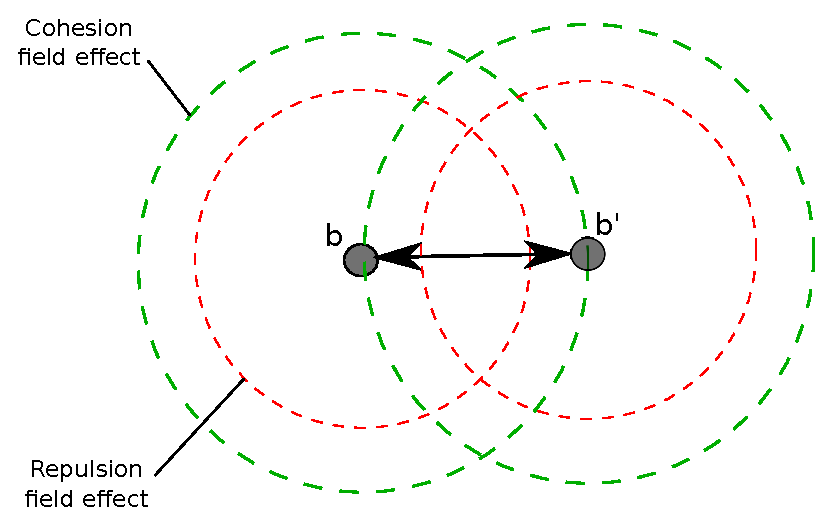
\includegraphics[width=9cm]{CHAPTER-9/figures/MagnitudeMetric1}
%% \end{center}
%% \caption{Magnitude Metric\label{additional:MagnitudeMetric1}}
%% \end{figure}

The chapter compares this new metric with the distance metric~(\autoref{section:DistanceDynamics}) currently in use and demonstrates how the \textit{inter-agent vector magnitude} is better suited to identifying the state of a swarm.  

%% \begin{figure}[H]
%% \begin{center}
%% 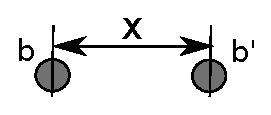
\includegraphics[width=3cm]{CHAPTER-9/figures/DistanceMetric1}
%% \end{center}
%% \caption{Distance metric\label{additional:DistanceMetric1}}
%% \end{figure}

The \textit{inter-agent vector} metric is based upon the component vectors that determine the inter-agent interactions rather than the resultant distribution of the agents. This change of focus creates a transferable metric that allows the effect of any field effect based algorithm to be analysed independently of the resultant distributions that the field effects create. The new metric also allows the `hidden potential' of a swarm to be identified. Inter-agent distance distribution does not show the underlying `potential' with respect to an agent's current vector magnitude state. The new metric allows a swarm to be identified as being in a repulsive state such that it will expand over time or as being in a cohesive state which results in the swarm remaining a single entity with a tendency to `stick' together. The application and benefits of the new metric are discussed further in~\autoref{additional:MoreWork}.

In chapter~\ref{chapter:SwarmType} the effect of varying the field effects of a swarm's agents and the impact this has on the swarm's structure is examined. The chapter demonstrates how the field effects can be used to produce different types of swarms based upon inter-agent `visibility'. The chapter demonstrates how the swarm models can be analysed using both the distance metric and the new \textit{inter-agent vector metric} defined in chapter~\ref{chapter:metric}. The chapter demonstrates how identifying the underlying inter-agent interactions allows the type of swarm to be identified and also highlights improvements that can be made in the field effects model to improve a swarm's structure. 

\subsection{Perimeter coordination}
If the application of a swarm requires it to move in a specific direction then an additional attribute must be added to the field effect model to create a goal based characteristic. In chapter~\ref{chapter:coordination} alternative swarm co-ordination algorithms are presented to create goal-based swarms capable of being applied to reconnaissance type tasks. The alternate methods are compared to a baseline static swarm to identify the effects the algorithms have upon a swarm's structure. The comparisons are carried out using both the distance-based metric and the new \textit{inter-agent vector magnitude} metric. This thesis explores three basic approaches to implementing a goal based characteristic. All agents using their GPS modules, only perimeter based agents using their GPS modules, and finally using a subset of the perimeter selected using a simple counting technique. The findings in this chapter are that by reducing the number of coordinator agents in a swarm it is possible to maintain a stable internal structure whilst imposing a directional bias to a swarm. The most effective technique is to use the smallest subset of the perimeter by using the basic count algorithm~(\autoref{section:stabilityComparison1}). The algorithm that produced the most internal disturbance is the `all agents' algorithm where all agents are coordinators. The chapter also examines the effects of balancing the field effects on a pro-rata basis (number of coordinators) to reduce the negative effects the algorithms can introduce. This is achieved by adjusting the individual vector component weightings for each of the algorithms used~(\autoref{sec:AlternateBias1}). When the \textit{weighting movement direction} parameters are altered the basic count mechanism is still the most effective algorithm~(\autoref{fig:BaselineAllMag100-60-20-2}).

\subsection{Concave reduction}
Chapter~\ref{chapter:ConcaveReduction} examines how swarms can exhibit emergent behaviours from a simple algorithm. A localised algorithm is used to improve inter-agent distributions by identifying gaps between an agent's neighbours and moving the agent towards the gap. This simple change to the swarming model produces two behavioural changes. It causes a swarm to close voids and migrate towards a more uniform shape. These effects can be interpreted as a `healing' effect as they cause the swarm to be more uniform in shape with no internal anomalies. This can be useful when a swarm's structure is disrupted by a failed agent or from disruptions to a swarm's path. This behaviour can also be applied to encapsulating an object. The object encapsulation effect is presented in terms of an existing application area in the petrochemical industry where they have identified the use of swarms as a potential method of controlling oil spillages~(\autoref{voids:ObjectSurrounding}). The technique used in this thesis uses a Boid-based swarming approach which differs to the current research which uses an ant-colony-based approach. This `healing' behaviour is also applied to goal-based swarms in an attempt to remove voids in a reconnaissance based swarm when a swarm's path is disrupted~(\autoref{concave:mobileSwarm1}). The thesis demonstrates that the emergent behaviour is able to remove a void created by an obstacle improving the coverage of the swarm's path using the \textit{concave-reduction} effect.

\subsection{Flood filling}
In chapter~\ref{chapter:flooding} the cohesion and repulsion field effects (\textit{interaction vectors}) are used to create an area filling behaviour using a swarm of a fixed size. This is achieved by increasing the repulsion field effect of the agents to influence the distribution of the agents such that the agents fill a bounded area. The chapter examines two different techniques of coordinating the expansion process. The first technique involves using a `normal' swarm that uses both cohesion and repulsion to create a swarm that acts as a single entity and ensures agents maintain `visibility' of each of its neighbours. The second technique exploits the fact that the swarm is in a bounded area and removes the cohesion field effect and uses only the repulsion field to expand the agents throughout the space. The metrics discussed in chapter~\ref{chapter:metric} are used to identify the effects of the expansion on the swarm's internal structures and to identify terminating conditions for the filling behaviours.

\section{Future work}\label{additional:MoreWork}
The research in this thesis has investigated several issues with respect to swarm analysis but has also raised further questions that need to be answered. The new metric allows swarms to be analysed in a completely different way and has opened up the possibility of analysing new swarm configurations.

\subsection{Magnitude metric application}\label{additional:fieldsWork}
Swarms are often constructed from heterogeneous agents that adapt to stimuli but the agents themselves are usually modelled using homogeneous field effects. This modelling of homogeneous field effects lends itself to being measured and monitored by a distance based metric as discussed by Navarro et al. \cite{NIM:09} and Gazi et al. (\cite{SALGVPJ:08, VG:05, GP:02, GP:04, GP:04a, GP:05, GP:11}) due to the regular shapes and structures that emerge. The dependence on regularity of shapes and structures is a limitation of the distance metric due to the aggregation of the distances not reflecting the mathematical model that creates the structures. The magnitude based metric overcomes that limitation by analysing the vectors that effect the agent distribution. With heterogeneous field effects the inter-agent distances may vary in an equilibrium state due to the way the field effects overlap when agents interact. 

The \textit{inter-agent vector magnitude} metric takes into consideration the resultant effects of the mathematical model rather than just arbitrary distances between agents. The balancing of \textit{interaction vectors} affect the resultant agent distributions.

The additional work required here would be to identify potential applications of these variations in the field effects that could improve existing swarm applications. For example, if an agent is on a perimeter would the swarm benefit from reducing the field effects to create a greater compression effect? Would having a mixed field effect swarm produce better coverage of an area? What would be the impact of having variable field effects upon a goal-based swarm?

\subsection{Area flooding}
If agents could vary their field effects based on their position in a swarm (e.g. agents at the boundary) is it possible to improve coverage?

If agents were able to vary their field effects based on detected environmental features a swarm may be able to achieve set goals more efficiently in unknown environments. An environment may have narrow paths linking larger chambers. Allowing agents to change their field effects may allow a swarm to propagate through this type of environment more effectively. This application requires further work to identify the effectiveness of using adaptive field effects on area flooding.
 
\subsection{Path following and shape forming swarms}\label{sec:DirectionalShape1}
The \textit{destination vector} as discussed in~\autoref{sec:Direction1} has been based upon a swarm having a fixed single destination however this model can be changed slightly to produce two more possible swarming effects by applying the \textit{destination vector} to a set of points. The effects that are possible are to create swarms that form arbitrary shapes or a swarm that will migrate along a specific path. The \textit{destination vector} required to achieve these two emergent behaviours can be implemented using the coordination techniques discussed in chapter~\ref{chapter:coordination}.

The main area of research that is still required in this area is how to best implement the coordination. The thesis shows that changing how coordination is applied via perimeter coordinators can improve a swarm's structure however what is not known is what is the best way to apply the coordination if a swarm is being applied to a shape forming~\cite{EP:07} or path following task.

\subsection{Self optimisation}\label{sec:Optimisation1}
The research carried out in terms of improving the performance of a swarm's
internal distribution shows that as the parameters are changed it is possile to
improve the performance of a swarm. Further work is therefore required to
identify what optimisation techniques could be applied to a swarm's algorithms
to improve its performance based on environmental conditions.

  %contribution 1
\chapter{Swarm movement metric}\label{chapter:metric}
%\section{Introduction\label{methods:SwarmStability}}
This chapter examines the distance metric as a mechanism to measure the internal movement of agents and introduces a new \textit{magnitude based metric}. The internal movement of a swarm is identified by analysing the changes in the inter-agent interactions. The two metrics differ in their approach to identifying the changes. The distance metric uses variations in the inter-agent spaces, as used by Navarro et al.~\cite{NIM:09}. The new metric, devised as part of this thesis, uses the magnitudes from the agents' \textit{inter-agent vectors} that are induced by agents' field effects as defined in~\autoref{eq:BotDirection3}. 

Both metrics allow a comparison of the effects of different swarming algorithms on a swarm's structure. The type of information that can be derived from each of the metrics is compared in~\autoref{metric:MagnitudeDistanceComparison}.

The magnitude based metric is used in chapter~\ref{chapter:coordination} to identify the effects of different coordination algorithms. In chapter~\ref{chapter:ConcaveReduction} the metric is used to identify the effects of both obstacles on a swarm's movement and the encapsulating behaviour a swarm exhibits when using \textit{concave reduction}.
 
%% \section{Metric principles\label{section:MagnitudeDynamics}}
%% This section discusses the theory behind swarm movement and the effects that can be measured using both the metrics described above.

\section{Inter-agent vector magnitude effect on internal movement}\label{Section:StabilityMagnitude}
\autoref{methods:Stability5} shows the cohesion and repulsion vector contributions to $v_c(b)$, $v_r(b)$ due to neighbour $b'$, as given in equations \ref{eq:FlyToCentre1}, \ref{eq:Repulsion1}. Notice that the vectors are along the line of separation $bb'$. 

Using the cohesion and repulsion vectors generated by the relationship of $b'$ to $b$ a resultant vector can be calculated. This vector creates an agent characteristic that can be used as a metric. Summing the vectors creates a resultant vector with a magnitude that affects the agent. Summing the vectors also provides an indication of the direction an agent will move based on the relationship. This is defined in chapter~\ref{chapter:methods} as the \textit{inter-agent vector}.

From here throughout \autoref{metric:MagnitudeDynamics2} and \autoref{metric:StabilityNullVector} imagine agent $b$ has just a single neighbour $b'$ and consider the effect of $b'$ on $v(b)$, the \textit{inter-agent vector} of $b$.
%% The relationship between the agents is that: \emph{the vector for $b$ with respect to $b^{'}$, and the vector for $b^{'}$ with respect to $b$ are on the same line}~(\autoref{methods:Stability5}).
%% If we consider an agent ($b$) as having only one neighbour ($b'$) then using the formulae defined in chapter~\ref{chapter:methods} the vectors $v_c(b)$~(\autoref{eq:FlyToCentre1}) and $v_r(b)$~(\autoref{eq:Repulsion1}) are the magnitudes of the vectors that are generated by the field effects between the two agents. $k_c$ and $k_r$ are the weighting factors for the cohesion and repulsion. The resulting vectors are aligned along the same line of separation between the agents. 

\begin{figure}[H]
\begin{center}
\includegraphics[width=7cm]{CHAPTER-4/figures/Stability5}
\end{center}
\caption{Vectors on line of separation} \label{methods:Stability5}
\end{figure}

\section{Swarm movement analysis\label{metric:MagnitudeDynamics2}}
The repulsive and cohesive vectors are generated for an agent through the intersection of their field effects~(\autoref{sec:Cohesion1} and \autoref{sec:Repulsion1}). There are a limited number of intersections that can occur; These are illustrated in Figures \ref{methods:Stability1}, \ref{methods:Stability2}, \ref{methods:Stability3}, \ref{methods:Stability4}.

Figures \ref{methods:Stability1}, \ref{methods:Stability2}, \ref{methods:Stability3}, \ref{methods:Stability4} show the cohesion of an agent pair as $k_cv_c$ and the repulsion as $k_rv_r$. The example data extracts~(Tables \ref{tab:SampleReplusion0}, \ref{tab:SampleReplusionPositive}, \ref{tab:SampleCohesionPositive}, \ref{tab:SampleEquilibrium}) are generated from the simulator using the parameters in table~\ref{tab:MetricPhysics1} that create a basic swarming behaviour. The tables show the simulation results. The simulation consists of 200 agents over a 20 second period. The simulation produces a neighbour extract of 248,798 records.

\begin{table}[H]
\begin{center}
\begin{tabular}{| p{2.5cm} | c | p{7cm} |}
\hline
\bf Weight \bf Component & \bf Swarm & \bf Description \\ \hline
Sample Rate & 100 & ms - Unit sampling interval\\  \hline
$k_c$ & 5 & weight adjuster for cohesion bias\\  \hline
$k_r$ & 15 & weight adjuster for repulsion  bias\\  \hline
$k_d$ & 0 & weight adjuster for directional bias 0 for static baseline 100 from directional\\  \hline
Repulsion field & 70 & units\\  \hline
Cohesion field & 80 & units\\  \hline
Speed & 20 & units/s\\  \hline
\end{tabular}\caption{Swarm parameters model} \label{tab:MetricPhysics1}
\end{center}
\end{table}

\autoref{methods:Stability1} shows two agents within each others cohesion fields but sufficiently distant to be outside of the repulsion fields. The `neighbour region' and `repulsion region' are the limits of the field effects for cohesion and repulsion. In this case $k_cv_c > 0$ and $k_rv_r = 0$: the result is the agent's resultant magnitudes cause the agents to move towards each other. \autoref{tab:SampleReplusion0} shows the repulsion magnitude with a value of 0. The only influence on the agent pairs are cohesive vectors. 

\begin{figure}[H]
\begin{center}
\includegraphics[width=11cm]{CHAPTER-4/figures/Stability1}
\end{center}
\caption{Internal movement cohesion (no repulsion)} \label{methods:Stability1}
\end{figure}

In tables~\ref{tab:SampleReplusion0},~\ref{tab:SampleReplusionPositive},~\ref{tab:SampleCohesionPositive}~and~\ref{tab:SampleEquilibrium}, \textbf{Log} is the sample identifier, \textbf{Id} is the unique identifier for an agent and \textbf{N.Id} is the Id of the agent neighbour. 

\begin{table}[H]
\begin{center}
\begin{tabular}{| l | l | l | l | l | l |}
\hline
Log &	Id &	N.Id &	Distance &	{\color{green}Cohesion} &	{\color{red}Repulsion} 	\\ \hline
0 &	1 &	3 	 & 70.50359957272653 &	{\color{green}352.5179978636327}  &	{\color{red}0} \\ \hline
0 &	1 &	100 & 71.78005530038806 &	{\color{green}358.9002765019403}  &	{\color{red}0} \\ \hline
0 &	1 &	151 & 78.33995887998715 &	{\color{green}391.69979439993574} &	{\color{red}0} \\ \hline
0 &	2 &	99  &	72.04066804327307 &	{\color{green}360.20334021636535} &	{\color{red}0} \\ 
\hline
\end{tabular}\caption{Data extract ($k_rv_r = 0$)} \label{tab:SampleReplusion0}
\end{center}
\end{table}

\autoref{methods:Stability2} shows two agents close together with repulsion dominating cohesion such that $k_cv_c < k_rv_r$. The resultant vector will direct the agents away from each other. \autoref{tab:SampleReplusionPositive} shows the repulsion magnitude with a value greater than cohesion.

\begin{figure}[H]
\begin{center}
\includegraphics[width=6.5cm]{CHAPTER-4/figures/Stability2}
\end{center}
\caption{Internal movement repulsion} \label{methods:Stability2}
\end{figure}

\begin{table}[H]
\begin{center}
\begin{tabular}{| l | l | l | l | l | l |}
\hline
Log &	Id &	N.Id &	Distance &	{\color{green}Cohesion} &	{\color{red}Repulsion} 	\\ \hline
0 & 1 &	2 &	28.325225929649267 &	{\color{green}141.62612964824635} &	{\color{red}1544.860149837827} \\ \hline
0 & 1 &	6 &	41.48517221724064  &	{\color{green}207.42586108620318} &	{\color{red}721.7173648240145} \\ \hline
0 & 1 &	7 &	35.264128136470426 & {\color{green}176.32064068235212} &	{\color{red}1034.271010913942} \\ \hline
0 & 1 &	8 &	43.545037655009644 &	{\color{green}217.72518827504823} &	{\color{red}637.9075999959364} \\
\hline
\end{tabular}\caption{Data extract ($|k_cv_c| < |k_rv_r|$)} \label{tab:SampleReplusionPositive}
\end{center}
\end{table}

\autoref{methods:Stability3} shows two agents close together but with cohesion vector magnitudes greater than the repulsion magnitudes $|k_cv_c| > |k_rv_r|$. The resultant vector will draw the agents together. The magnitude of the resultant cohesion vector will be reduced due to the cancelling effect of the repulsion vector. \autoref{tab:SampleCohesionPositive} shows a data extract with the cohesion magnitude greater than repulsion.

\begin{figure}[H]
\begin{center}
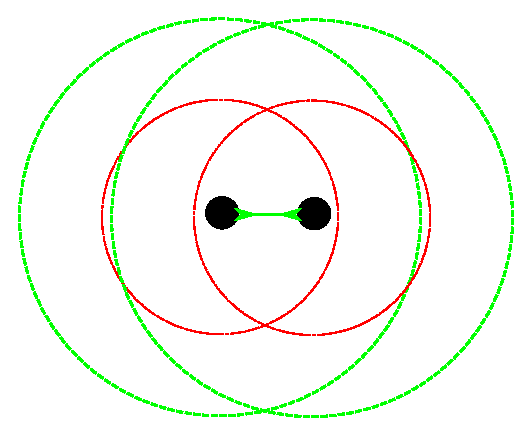
\includegraphics[width=6.5cm]{CHAPTER-4/figures/Stability3}
\end{center}
\caption{Internal movement cohesion} \label{methods:Stability3}
\end{figure}

\begin{table}[H]
\begin{center}
\begin{tabular}{| l | l | l | l | l | l |}
\hline
Log &	Id &	N.Id &	Distance &	{\color{green}Cohesion} &	{\color{red}Repulsion} 	\\ \hline
0 &	1 &	5 &	64.17214469587854 &	{\color{green}320.86072347939273} & 	{\color{red}95.35676418993891} \\ \hline
0 &	1 &	9 &	63.880497718571355 &	{\color{green}319.4024885928568} &	{\color{red}100.58590062663305} \\ \hline
0 &	1 &	95 &	65.6152270119206 &	{\color{green}328.07613505960296} & 	{\color{red}70.16681717258929} \\ \hline
0 &	1 &	152 &	63.10700566424517 &	{\color{green}315.53502832122587} & 	{\color{red}114.68844031437281} \\ 
\hline
\end{tabular}\caption{Data extract ($|k_cv_c| > |k_rv_r|$)} \label{tab:SampleCohesionPositive}
\end{center}
\end{table}

\autoref{methods:Stability4} shows two agents close together with $|k_cv_c| = |k_rv_r|$ the resultant vector will be a \textit{null vector} and the agents will have no influence upon each other due to the magnitude of the resultant vector being zero. \autoref{tab:SampleEquilibrium} is an extract from the \textbf{\texttt{NEIGHBOURS}} table. The data shows an extract that is near equilibrium. The simulation produced no null magnitude results. 

\begin{figure}[H]
\begin{center}
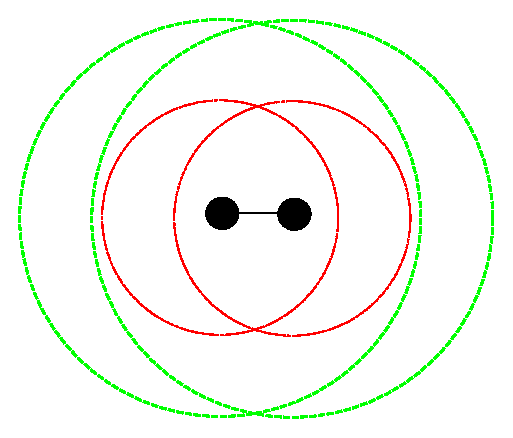
\includegraphics[width=6.5cm]{CHAPTER-4/figures/Stability4}
\end{center}
\caption{Internal movement equilibrium} \label{methods:Stability4}
\end{figure}

\begin{table}[H]
\begin{center}
\begin{tabular}{| l | l | l | l | l | l |}
\hline
Log &	Id &	N.Id &	Distance &	{\color{green}Cohesion} &	{\color{red}Repulsion} 	\\ \hline
7 &	76 &	91 &	55.390312278311875 &	{\color{green}276.9515613915594} &	{\color{red}276.9468428106153} \\ \hline
24 &	75 &	6 &	55.39032191143417 &	{\color{green}276.95160955717085} &	{\color{red}276.9466120367043} \\ \hline
32 &	72 &	38 &	55.39002603773678 &	{\color{green}276.9501301886839} &	{\color{red}276.95370011064875} \\ \hline
35 &	63 &	64 & 	55.390227283173054 &	{\color{green}276.9511364158653} &	{\color{red}276.9488789826377} \\
\hline
\end{tabular}\caption{Data extract ($|k_cv_c| \approx |k_rv_r|$)} \label{tab:SampleEquilibrium}
\end{center}
\end{table}

\section{Internal movement and the null vector}\label{metric:StabilityNullVector}
When the two vectors (cohesion and repulsion) have magnitudes that are equal and opposite they produce a null vector. This indicates that two agents are optimally spaced for a given set of conditions. Although the agents are at an optimum position it does not mean the swarm is optimally distributed. If a swarm is in a confined space it is possible for an optimum position to be created where the vector magnitude is positive due to a compression effect. This phenomenon is used in the identification of the emergent behaviour of area flooding, covered in chapter~\ref{chapter:flooding}.  

If we consider the equilibrium state (\autoref{methods:Stability4}) the resultant vector of $b$ is $(0,0)$. A null vector cannot be normalised to produce a directional vector ($\hat{v} = \frac{v}{|v|}$ if $v\neq0$; $0$ if $v=0$). The effect of the resultant magnitude being a null vector is that the agent will remain stationary. If all agent pairs are in this condition the swarm will stop moving~(\autoref{methods:StabilityNullVector}).

\begin{figure}[H]
\begin{center}
\includegraphics[width=7cm]{CHAPTER-4/figures/StabilityNullVector}
\end{center}
\caption{Equilibrium with null vectors} \label{methods:StabilityNullVector}
\end{figure}

Due to the independent nature of the agents this situation is very rare. The residual motion that persists in a swarm is the background `noise' or `jitter' that an algorithm creates.

If a swarm is goal-based the additional \textit{directional vector} will prevent all agents simultaneously producing null vectors~(\autoref{methods:StabilityNullVector2}).

\begin{figure}[H]
\centering
\subfigure[($t$)]{
	 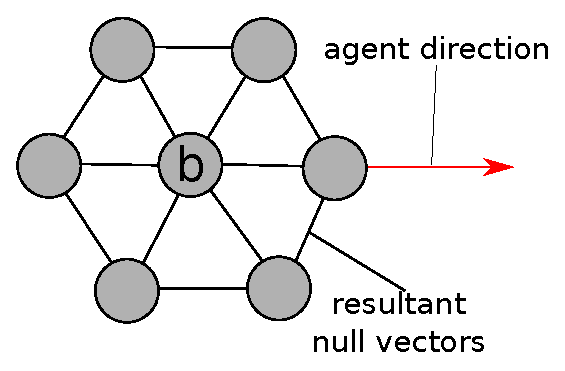
\includegraphics[width=5.5cm]{CHAPTER-4/figures/StabilityNullVector3}
    \label{concave:VoidPerimeter1}
}
\subfigure[($t + 1$)]{
	 \includegraphics[width=6cm]{CHAPTER-4/figures/StabilityNullVector2}
    \label{concave:VoidPerimeter2}
}
\caption{Directional movement and the null vector}
\label{methods:StabilityNullVector2}
\end{figure}

\section{Residual internal movement (Jitter)}\label{metric:Jitter}
Due to the dynamic nature of a swarm maintaining optimum internal movement as in~(\autoref{methods:Stability4}) a stationary swarm is highly unlikely. The agent pairs will fluctuate between the 3 states~(Figures~\ref{methods:Stability2}, \ref{methods:Stability3}, \ref{methods:Stability4}). This alternation between the states is \textit{jitter}. The degree to which this variation occurs can be measured using either the change in distance between the agent pairs, or the change in the resultant magnitude between the agent pairs. Jitter is motion that is produced to maintain the structure of a swarm. A coordination algorithm that produces minimal jitter is generally more desirable. Jitter (the fluctuation in and between the states) is an indication of the efficiency of an algorithm and an integral component of a swarm's measurable behaviour.

\section{Magnitude based metric\label{section:MagnitudeDynamics}}
Magnitude based internal movement (\textit{agent resultant magnitude}) is measured by identifying the balance between the repulsion and cohesion between agents. `Jitter' in the case of the \textit{agent resultant magnitude} metric is measured as the variance of the potentials created by the agents. The identification of this variance produces the clarifying part of the \textit{agent resultant magnitude} metric.
%% The magnitude based metric identifies the resultant internal magnitude (vector magnitude) through the cohesive and repulsive magnitudes that exist between each agent pair in a swarm. 
The \textit{agent resultant magnitude} is identified by Gazi and Passino~\cite{GP:11} and Barnes et al~\cite{BFV:07} as a `resultant characteristic' of a swarm. There are two ways of using the cohesion and repulsion in identifying a resultant vector. The two vectors can be added as absolute values to give an overall `size' to the magnitude that is affecting each relationship. Alternatively the resultant magnitude can be the sum of the actual magnitudes. The repulsion vector has a negative magnitude and the cohesion vector has a positive magnitude. In this thesis the magnitude analysis will be based on summing the two actual vectors to determine the result of the inter-agent interaction. This thesis will refer to the resultant magnitude as the \text{`agent resultant magnitude'} of the relationship. The `state' of a swarm is the effect the environmental constraints and algorithms have upon the agent resultant magnitude. It is a part of the `quality' measure for a swarm's performance.

If the \textit{agent resultant magnitude} is a negative value (absolute values would prevent this analysis) the swarm's bias is to expand. This is seen in the disorganised stage of a swarm. If the \textit{agent resultant magnitude} is positive then the swarm is exhibiting a tendency to contract and this indicates the swarm is a cohesive entity. This could also be described as the swarm being `sticky' as the agents bias is to `pull' towards each other.

The \textit{agent resultant magnitude} on its own does not give a complete measure of a swarm's internal state. There needs to be a qualifying component to the metric  that identifies the degree of deviation in the resultant magnitude, this is the \textit{jitter}. The smaller the degree of deviation the more uniform the structure of the swarm. These two components identify the degree to which a swarm has progressed towards a stable state. 

The \textit{agent resultant magnitude} provides a view of the swarm's state through the balance between the repulsive and the cohesive vectors that are being applied to each agent. The variance component identifies the degree to which the swarm has stabilised. The ideal status for inter-agent interactions would be for the agents to have a resultant vector (\textit{agent resultant magnitude}) of zero or above. This would indicate that the agents are distributed such that they are at their distribution limit (outer most range of the cohesion field) or at a level that causes the agents to `pull' together. The ideal degree of deviation is zero as this indicates an even distribution of agents. Therefore for a fuller indication of a swarm's \textit{state} both measurements need to be combined. The deviation from the mean clarifying the internal movement and the \textit{agent resultant magnitude} providing an indication of the `compression' that a swarm is logically experiencing (cohesiveness). These two aspects of a swarm's features are not considered by Gazi and Passino~\cite{GP:11} or Barnes et al~\cite{BFV:07} as a means of quantifying the structure of a swarm in terms of stability.

\section{Distance based metric\label{section:DistanceDynamics}}
The distance based metric considers the effect of the resultant vectors upon a swarm in terms of how the agents are physically distributed: i.e. only the inter-agent distances and the deviation from the mean of the agents (jitter) are considered. As with the \textit{agent resultant magnitude} metric the variations are important to determine the agent distribution. The standard deviation from the mean allows the internal `characteristic' of the measure to be realised. If the standard deviation is zero then all the agents are evenly spaced. The distance metric does not take into consideration the vector magnitudes between the agents as discussed above. The metric therefore is unable to identify the potential state of the swarm in terms of its cohesive or repulsive state.

Navarro and Fernando describe a mean distance error metric that is based on the variations in distances between inter-agent spaces~\cite{NIM:09}. This is the same as the standard deviation of the distance based internal movement metric as described here. 

\section{Magnitude based internal movement model}\label{Section:StabilityModel}
Using the formulae for the calculation of cohesion~(\autoref{eq:FlyToCentre1}, page \pageref{eq:FlyToCentre1}) and repulsion~(\autoref{eq:Repulsion1}, page \pageref{eq:Repulsion1}) for every agent and its neighbours it is possible to calculate an \textit{agent resultant magnitude} value (sum of agent resultant magnitudes). This value represents the overall potential of an agent. This magnitude when normalised produces a component of the \textit{movement-destination vector}~(\autoref{eq:BotDirection1}) for a swarm. If the agent resultant magnitude is zero (null vector) then the agent will not move. $P(b)$ is the \textit{inter-agent resultant magnitude vector} for agent $b$ defined by:

\begin{equation}
\label{eq:BotStabilityT}
P(b) = k_cv_c(b) + k_r v_r(b)
\end{equation}

Although it is possible for agent $b$ to have a resultant vector of null there could still be a variation in the constituent components. The variation calculation (standard deviation) is shown in~\autoref{Section:VarianceInPotential}. \autoref{eq:SwarmStabilityMetricT} is the mean of the \textit{agent resultant magnitudes} for an agent and its neighbours where $\card{nbr(b)}$ is the number of neighbours.

\begin{equation}
\label{eq:SwarmStabilityMetricT}
\mu_p(b) = \frac{P(b)}{\card{nbr(b)}}
\end{equation}

%% \autoref{eq:SwarmStabilityMetricT} should be considered as being applied at discrete points in time within a simulation. The formulae could also be shown based on time $t$ (\autoref{eq:SwarmStabilityMetricT2}) where $b_t$ is an agent at a specific time interval. All formulae for agent resultant magnitude in this thesis will be considered as being applied at a point in time and will therefore be shown without a $t$ subscript.
%% 
%% \begin{equation}
%% \label{eq:SwarmStabilityMetricT2}
%% \mu_p(b_{t}) = \frac{P(b_{t})}{|nbr(b_{t})|}
%% \end{equation}

To identify the swarm based \textit{agent resultant magnitude}~\autoref{eq:SwarmStabilityMetricT} must be extended to iterate over all the agents in the swarm. \autoref{eq:SwarmStabilityMetricT3} shows $\mu_p(S)$~as the swarm based magnitude where the swarm iteration is shown as~$\sum_{b \in S}$ and $\sum_{b \in S}\card{nbr(b)}$ calculates the total number of inter-agent relationships.

\begin{equation}
\label{eq:SwarmStabilityMetricT3}
\mu_p(S) = \frac{\mathlarger{\sum_{b \in S} P(b)}}{\mathlarger{\sum_{b \in S}}\card{nbr(b)}}
\end{equation}

\section{Variance in agent resultant magnitude metric}\label{Section:VarianceInPotential}
The mechanism just described provides an overall indication of the internal movement based on inter agent vectors that produce the \textit{agent resultant magnitude}. This model however is not sufficient to give an indication of the swarm `state' as an overall metric. To improve the metric clarification is required in terms of the deviation from the \textit{agent resultant magnitude} norm. The variation in the metric is the standard deviation of the entire swarm from the mean of the inter-agent potential magnitudes (\autoref{eq:SwarmStabilityMetricT}).

The standard deviation is calculated as~\autoref{eq:SwarmStabilityQuotientT} where $\sigma_p(S)$ is the standard deviation at a time $t$ and $\mu_p(S)$ is the mean at the same point in time. $\sum_{b \in S}~\sum_{b' \in nbr(b)}$ iterates over every agent in the swarm and its neighbours and $\sum_{b \in S}\card{nbr(b)}$ calculates the total number of inter-agent relationships.

\begin{equation}
\label{eq:SwarmStabilityQuotientT}
\sigma_p(S) = \sqrt{\frac{\mathlarger{\sum_{b \in S}}~\mathlarger{\sum_{b' \in nbr(b)}}\Big(P(b')-\mu_p(S)\Big)^2}{\mathlarger{\sum_{b \in S}}\card{nbr(b)}}}
\end{equation}

The metric for the internal movement is a set of numbers, the mean and standard deviation of the swarm's internal \textit{agent resultant magnitude} derived from each agent and its neighbour interactions~(\autoref{eq:SwarmPotentialMagnitude}). The pair $\mu_p(S)$, $\sigma_p(S)$ may be written informally as: 

\begin{equation}
\label{eq:SwarmPotentialMagnitude}
\psi_p = \mu_p(S)\pm \sigma_p(S)
\end{equation}

\section{Distance metric}
The distance based internal movement is measured by identifying the mean length of the vectors between an agent and its neighbours. As with the \textit{agent resultant magnitude} a coordination algorithm produces `jitter' which is the variations from the mean. In the case of the distance based metric the jitter is identified by the changes in the distances rather than the changes in vector magnitude (\textit{agent resultant magnitude}). The distance metric is the mean and the standard deviation `jitter' of the inter-agent distances.

\section{Calculating distance based internal movement}
The relative position vector generated for an agent $b$ to its neighbour $b'$, $bb'$, is shown in~(\autoref{eq:FlyToCentre1}). The magnitude of that vector gives the distance between two agents. For an individual agent the average magnitude $\mu_d(b)$ is calculated as \autoref{eq:SwarmStabilityDistance1} where $b$ is the agent and $\card{nbr(b)}$ is the number of neighbours.

\begin{equation}
\label{eq:SwarmStabilityDistance1}
\mu_d(b) = \frac{\mathlarger{\sum_{b' \in nbr(b)}}\magn{bb'}}{\mathlarger{\card{nbr(b)}}}
\end{equation}

\label{eq:SwarmStabilityDistance1} identifies the mean distance for an individual agent. The mean distance for a swarm is calculated by \autoref{eq:SwarmStabilityDistance2}. All the inter-agent interactions must be included for the swarm ($S$). $\sum_{b \in S}|nbr(b)|$ calculates how many inter-agent relationships exist in the swarm and $\sum_{b' \in nbr(b)}\magn{bb'}$ calculates the total distance between each agent and its neighbours. $\sum_{b \in S}$ iterates over all the agents in the swarm~($S$).

\begin{equation}
\label{eq:SwarmStabilityDistance2}
\mu_d(S) = \frac{\mathlarger{\sum_{b \in S}}~\mathlarger{\sum_{b' \in nbr(b)}}\magn{bb'}}{\mathlarger{\sum_{b \in S}\card{nbr(b)}}}
\end{equation}

\section{Variance in distance metric}\label{Section:VarianceInDistance}
The mechanism above provides an overall indication of the distribution of the agents. This model, as with the agent resultant magnitude model, is not sufficient to give an indication of the internal distribution of the agents. The addition of the standard deviation from the norm clarifies the distribution within the swarm as shown in~equation~\ref{eq:SwarmStabilityDistance3}. $(\magn{bb'} - \mu(S))^2$ is the square of the difference in a distance to the mean and $\sum_{b \in S}~\sum_{b' \in nbr(b)}$ calculates the number of inter-agent interactions.

\begin{equation}
\label{eq:SwarmStabilityDistance3}
\sigma_d(S) = \sqrt{\frac{\mathlarger{\sum_{b \in S}}~\mathlarger{\sum_{b' \in nbr(b)}}\Big(\magn{bb'} - \mu_d(S)\Big)^2}{\mathlarger{\sum_{b \in S}\card{nbr(b)}}}}
\end{equation}

The distance metric for the internal distribution of the agents is the pair consisting of $\mu_d(S)$, $\sigma_d(S)$ the mean and the standard deviation of the swarm's internal resultant distances from every agent in the swarm. This can be written informally as:

\begin{equation}
\label{eq:SwarmPotentialMagnitude}
\psi_d = \mu_d(S)\pm \sigma_d(S)
\end{equation}

\section{Conclusion - metric comparison\label{metric:MagnitudeDistanceComparison}}
The two metrics appear to be similar in terms of the measurement of the structure of a swarm. The main difference is in how these two metrics can be used when examining the state of the swarm.

Both metrics identify the state of a swarm with respect to variations in the dispersement of the agents from an average distribution. 

The main difference in the metrics is that the distance metric is based upon the physical \textit{distribution} of the agents and the magnitude based metric is based upon the logical \textit{interaction} of the agents.

The distance based metric provides and analysis of the actual distribution of the agents at a point in time and allows the agitation of the swarm to be assessed without considering the possible distribution of agents that the field effects \textit{could} produce.

The \textit{agent resultant magnitude} metric provides a view of the interaction magnitude. This provides an indication of the swarm's potential movement. This is independent of the physical distribution. The lack of dependence on the physical distribution allows the metric to be used in heterogeneous field effect swarms~\autoref{additional:fieldsWork} where the physical distribution may vary. 

Combining the two metrics allows a deeper evaluation of a swarm to be made. Consider the following: the repulsion field is increased but the internal distances do not change as a result the \textit{agent resultant magnitude} rises: This indicates `something' is confining the swarm's distribution. This analysis could be used in identifying effective swarm distribution for the coverage of a sensor array as discussed by Ramaithitima et al.~\cite{RWBK:15}
  %contribution 2
\chapter{Swarm type identification}\label{chapter:SwarmType}
%%\section{Metric application - swarm type identification\label{methods:SwarmTypesStability1}}
This chapter applies the metrics defined in chapter~\ref{chapter:metric} to identify how the cohesion and repulsion field effects of the \textit{interaction vector} affect the internal movement and the vector magnitudes between agents in a swarm. 

There are two distinct inter-agent structures that can emerge in a boid-based swarm, \textit{hexagonally-connected} or \textit{hyper-connected}. These two swarm types are the result of the cohesion field effect detecting immediate neighbours only and when the neighbour field effect range extends beyond immediate neighbours to include additional agents. 

If the goal is to maximise the coverage of an area by a swarm's agents then a hexagonal lattice is the most appropriate structure. In a \textit{hexagonally-connected} swarm agents have visibility only of their immediate neighbours and are unaffected by agents beyond those neighbours. This effect can be implemented by ignoring agents beyond the initial neighbours detected or confining the field effects such that the connections do not occur. If the field effects extend beyond the immediate neighbours such that further agents are detected then there will be additional vectors affecting the calculations of an agent's \textit{interaction vectors}. These additional vectors cause the structure to change logically from a lattice to a mesh. A mesh structure is a \textit{hyper-connected} swarm.

\section{Internal movement testing (static swarms)}\label{Section:StabilityTesting}
To evaluate the metrics simulation parameters (field effects) need to be created such that they generate the two swarm types~(\autoref{tab:Physics2}).

Table~\ref{tab:Physics2} shows the parameter requirements for two swarm types. The parameters in the \textit{Hexagonal} column generate a swarm structure where an agent can only detect immediate neighbours. The parameters in the \textit{Hyper} column allow agents to detect agents beyond their immediate neighbours and therefore create additional neighbour connections which results in a hyper-connected swarm.

\begin{table}[H]
\begin{center}
\begin{tabular}{| p{2.5cm} | K{2.5cm} | K{2.5cm} | p{4.5cm} |}
\hline
\bf Weight \bf component & \bf Hexagonal \bf Swarm & \bf Hyper \bf connected & \bf Description \\ \hline
Sample Rate & 100 & 100 & ms - Unit sampling interval\\  \hline
$k_c$ & 5 & 5 & weight adjuster for cohesion bias\\  \hline
$k_r$ & 15 & 15 & weight adjuster for repulsion  bias\\  \hline
$k_d$ & 0 & 0 & weight adjuster for directional bias\\  \hline
Cohesion field & 50 & 60 &  units\\  \hline
Repulsion field & 40 & 40 & units\\  \hline
Speed & 20 & 20 & units/s\\  \hline
\end{tabular}\caption{Swarm Weighted Model} \label{tab:Physics2}
\end{center}
\end{table}

The two sets of parameters are simulated using a swarm of 200 agents randomly distributed in an environment. The simulation generates data as described in chapter~\ref{chapter:simulator}. The data extracts contain the distances and inter-agent magnitudes (\textit{interaction vectors}) produced by the parameters.

\section{Hexagonal swarm analysis}\label{section:AnalysisA}
In a hexagonal swarm the field effects cause the agents to form a regular lattice. All the agents tend towards an even distributed with similar distances between each agent and its neighbours. In a well structured deployment, the agents in the swarm will show limited variation in the inter-agent distances and the \textit{interaction vectors}. A perfect distribution is very unlikely in a swarm of agents due to the constant movement of the agents adjusting their positions to obtain an optimum position and the agents moving at a constant speed.

\subsection{Distance based metric}
The distance analysis graph~(\autoref{methods:StabilityDistanceSwarm40-50}) for the hexagonal swarm (using the parameters in Table~\ref{tab:Physics2}, repulsion field 40 units, cohesion field 60 units) shows the distance metric being applied to the swarm over a period of 200 cycles. The graph shows a trace of the distance with the standard deviation displayed as error bars above and below the mean.

The swarm is initially (0-20 cycles) in a state of disorganisation, where the agent distribution is varied. The swarm then enters a phase where the hexagons are forming and the swarm starts to stablise (20-50 cycles). After about 50 cycles the field effects have stabilised the swarm structure and the swarm settles to a more stable state for the given set of parameters. The swarm then fluctuates as the residual internal movement maintains the swarms structure. At this point the internal movement (jitter) is the `background noise' generated by the field effects to maintain the swarm's structure.

%HEX-DIST.py
\begin{figure}[H]
\begin{center}
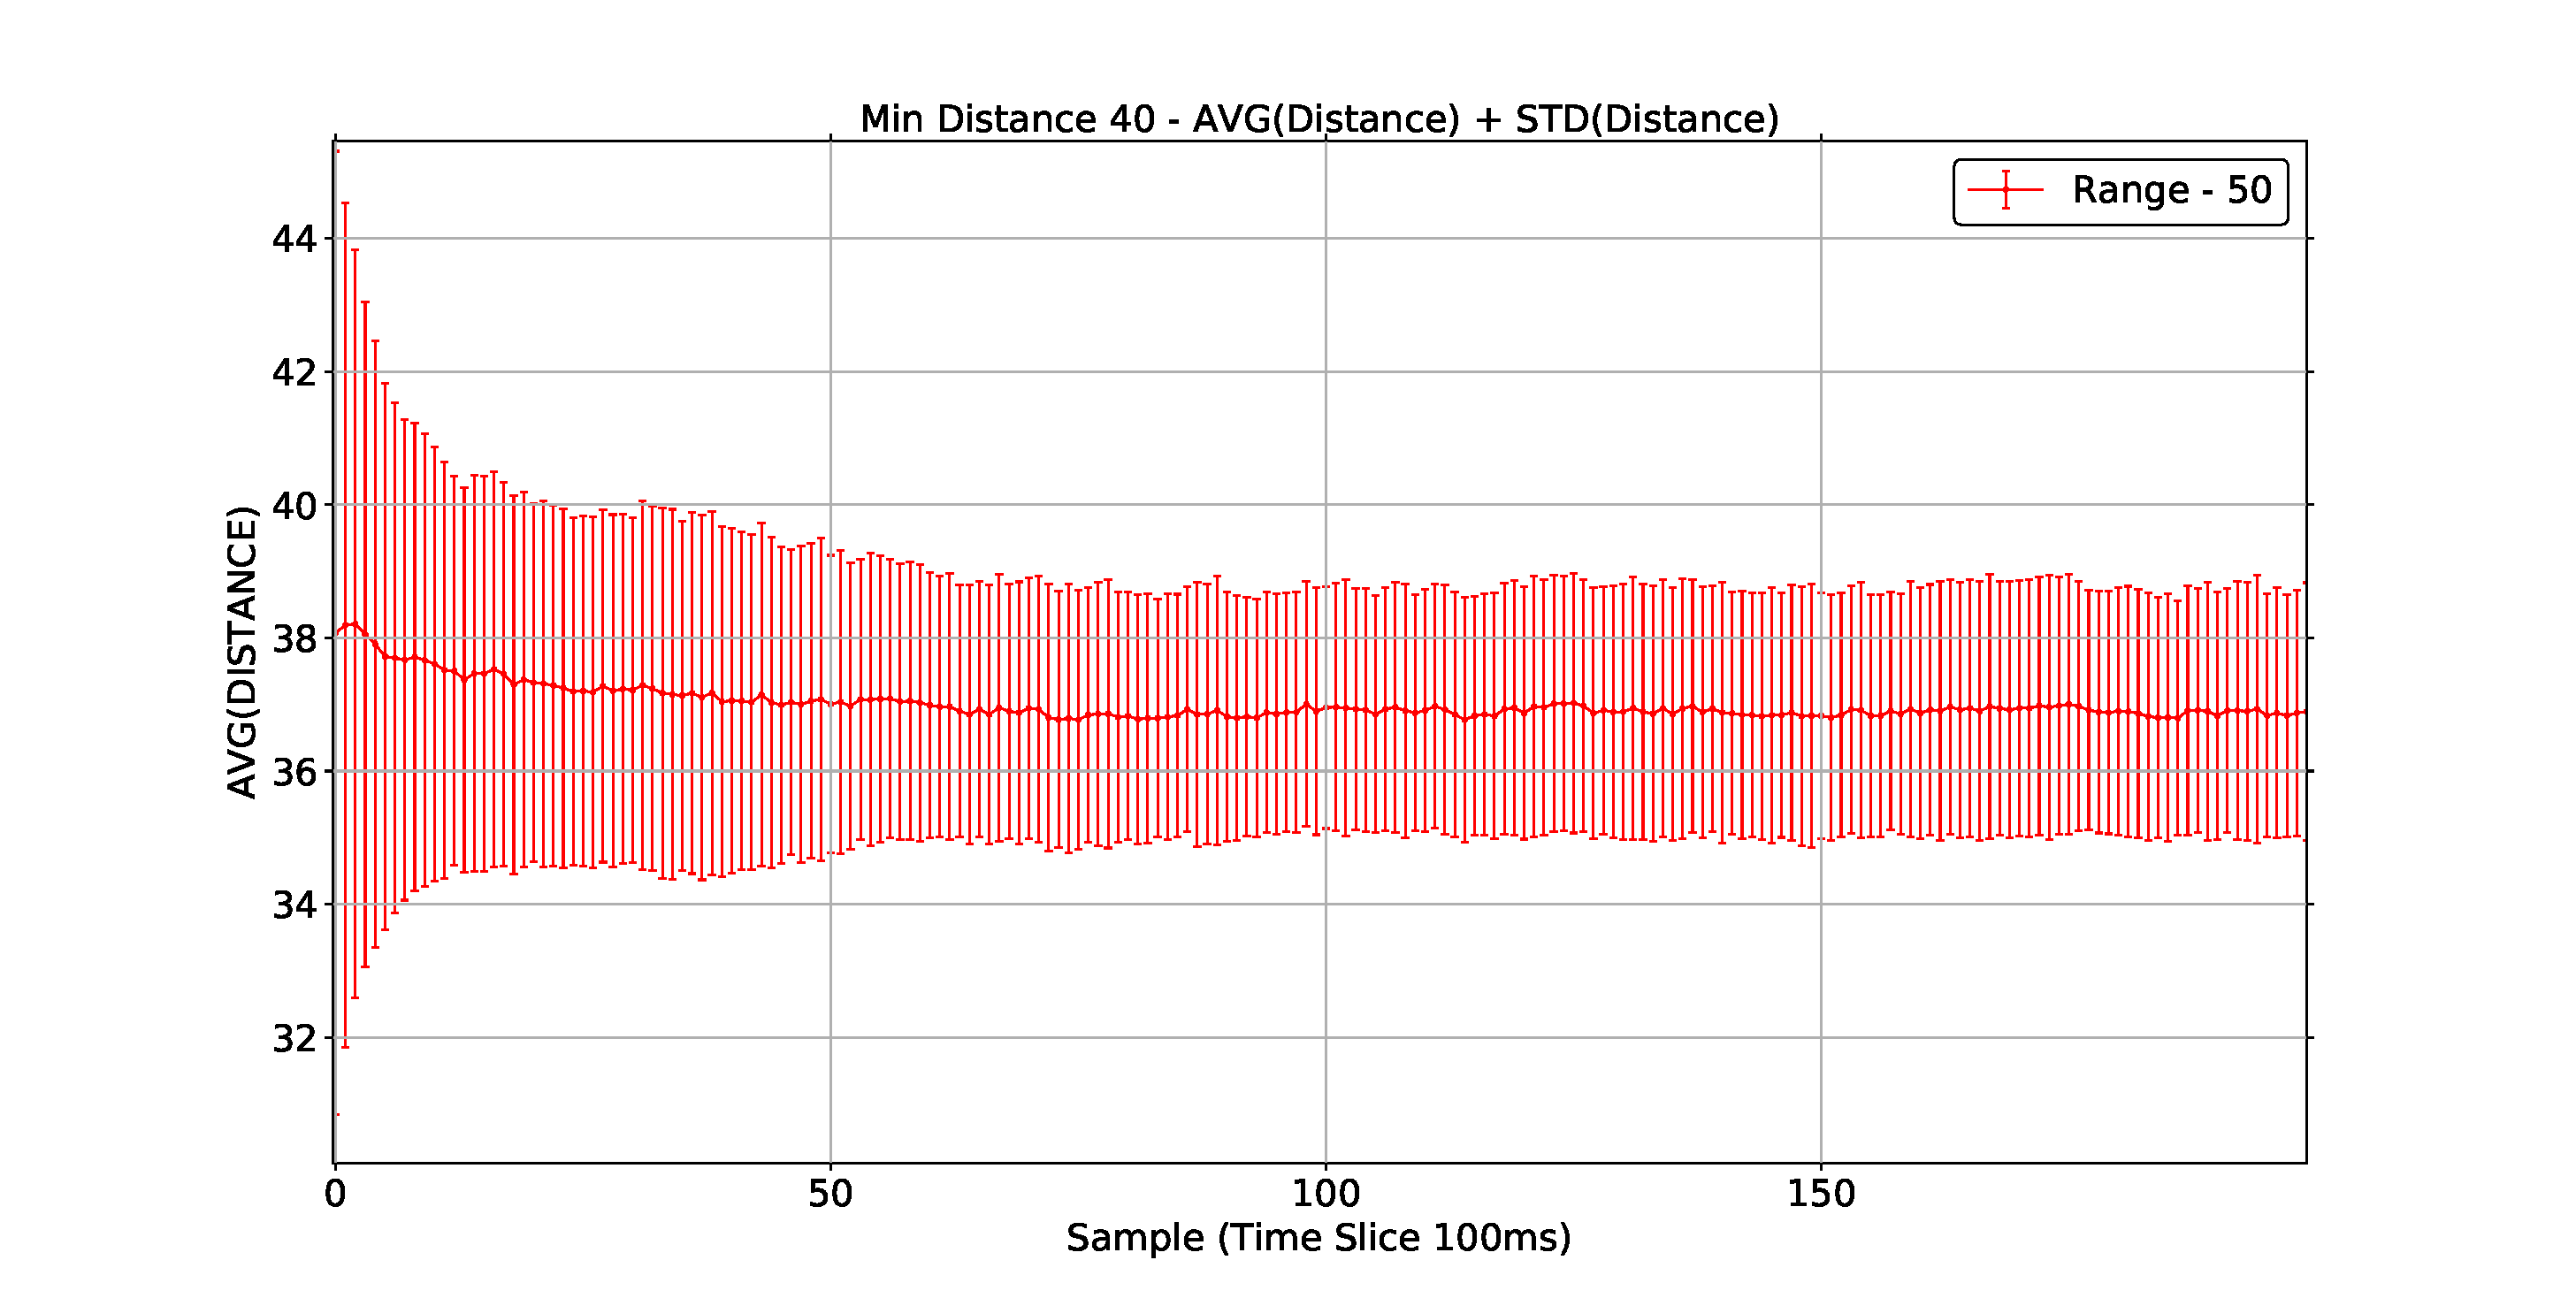
\includegraphics[width=13cm]{CHAPTER-5/figures/StabilityDistanceSwarm40-50}
\end{center}
\caption{Hexagonal swarm - distance metric\label{methods:StabilityDistanceSwarm40-50}}
\end{figure}

\autoref{methods:StabilityDistributionHexagonal}~shows the distribution of the inter-agent distances for the duration of the simulation. The data forms a bell shaped distribution with a mean distance of approximately 37 units, the mean distance is the average of all the inter agent distances as shown in \autoref{methods:StabilityDistanceSwarm40-50}. The graph shows the changes in the distribution of distances based on the aggregation of the whole simulation. 
%HEX-DIST-BAR.py
\begin{figure}[H]
\begin{center}
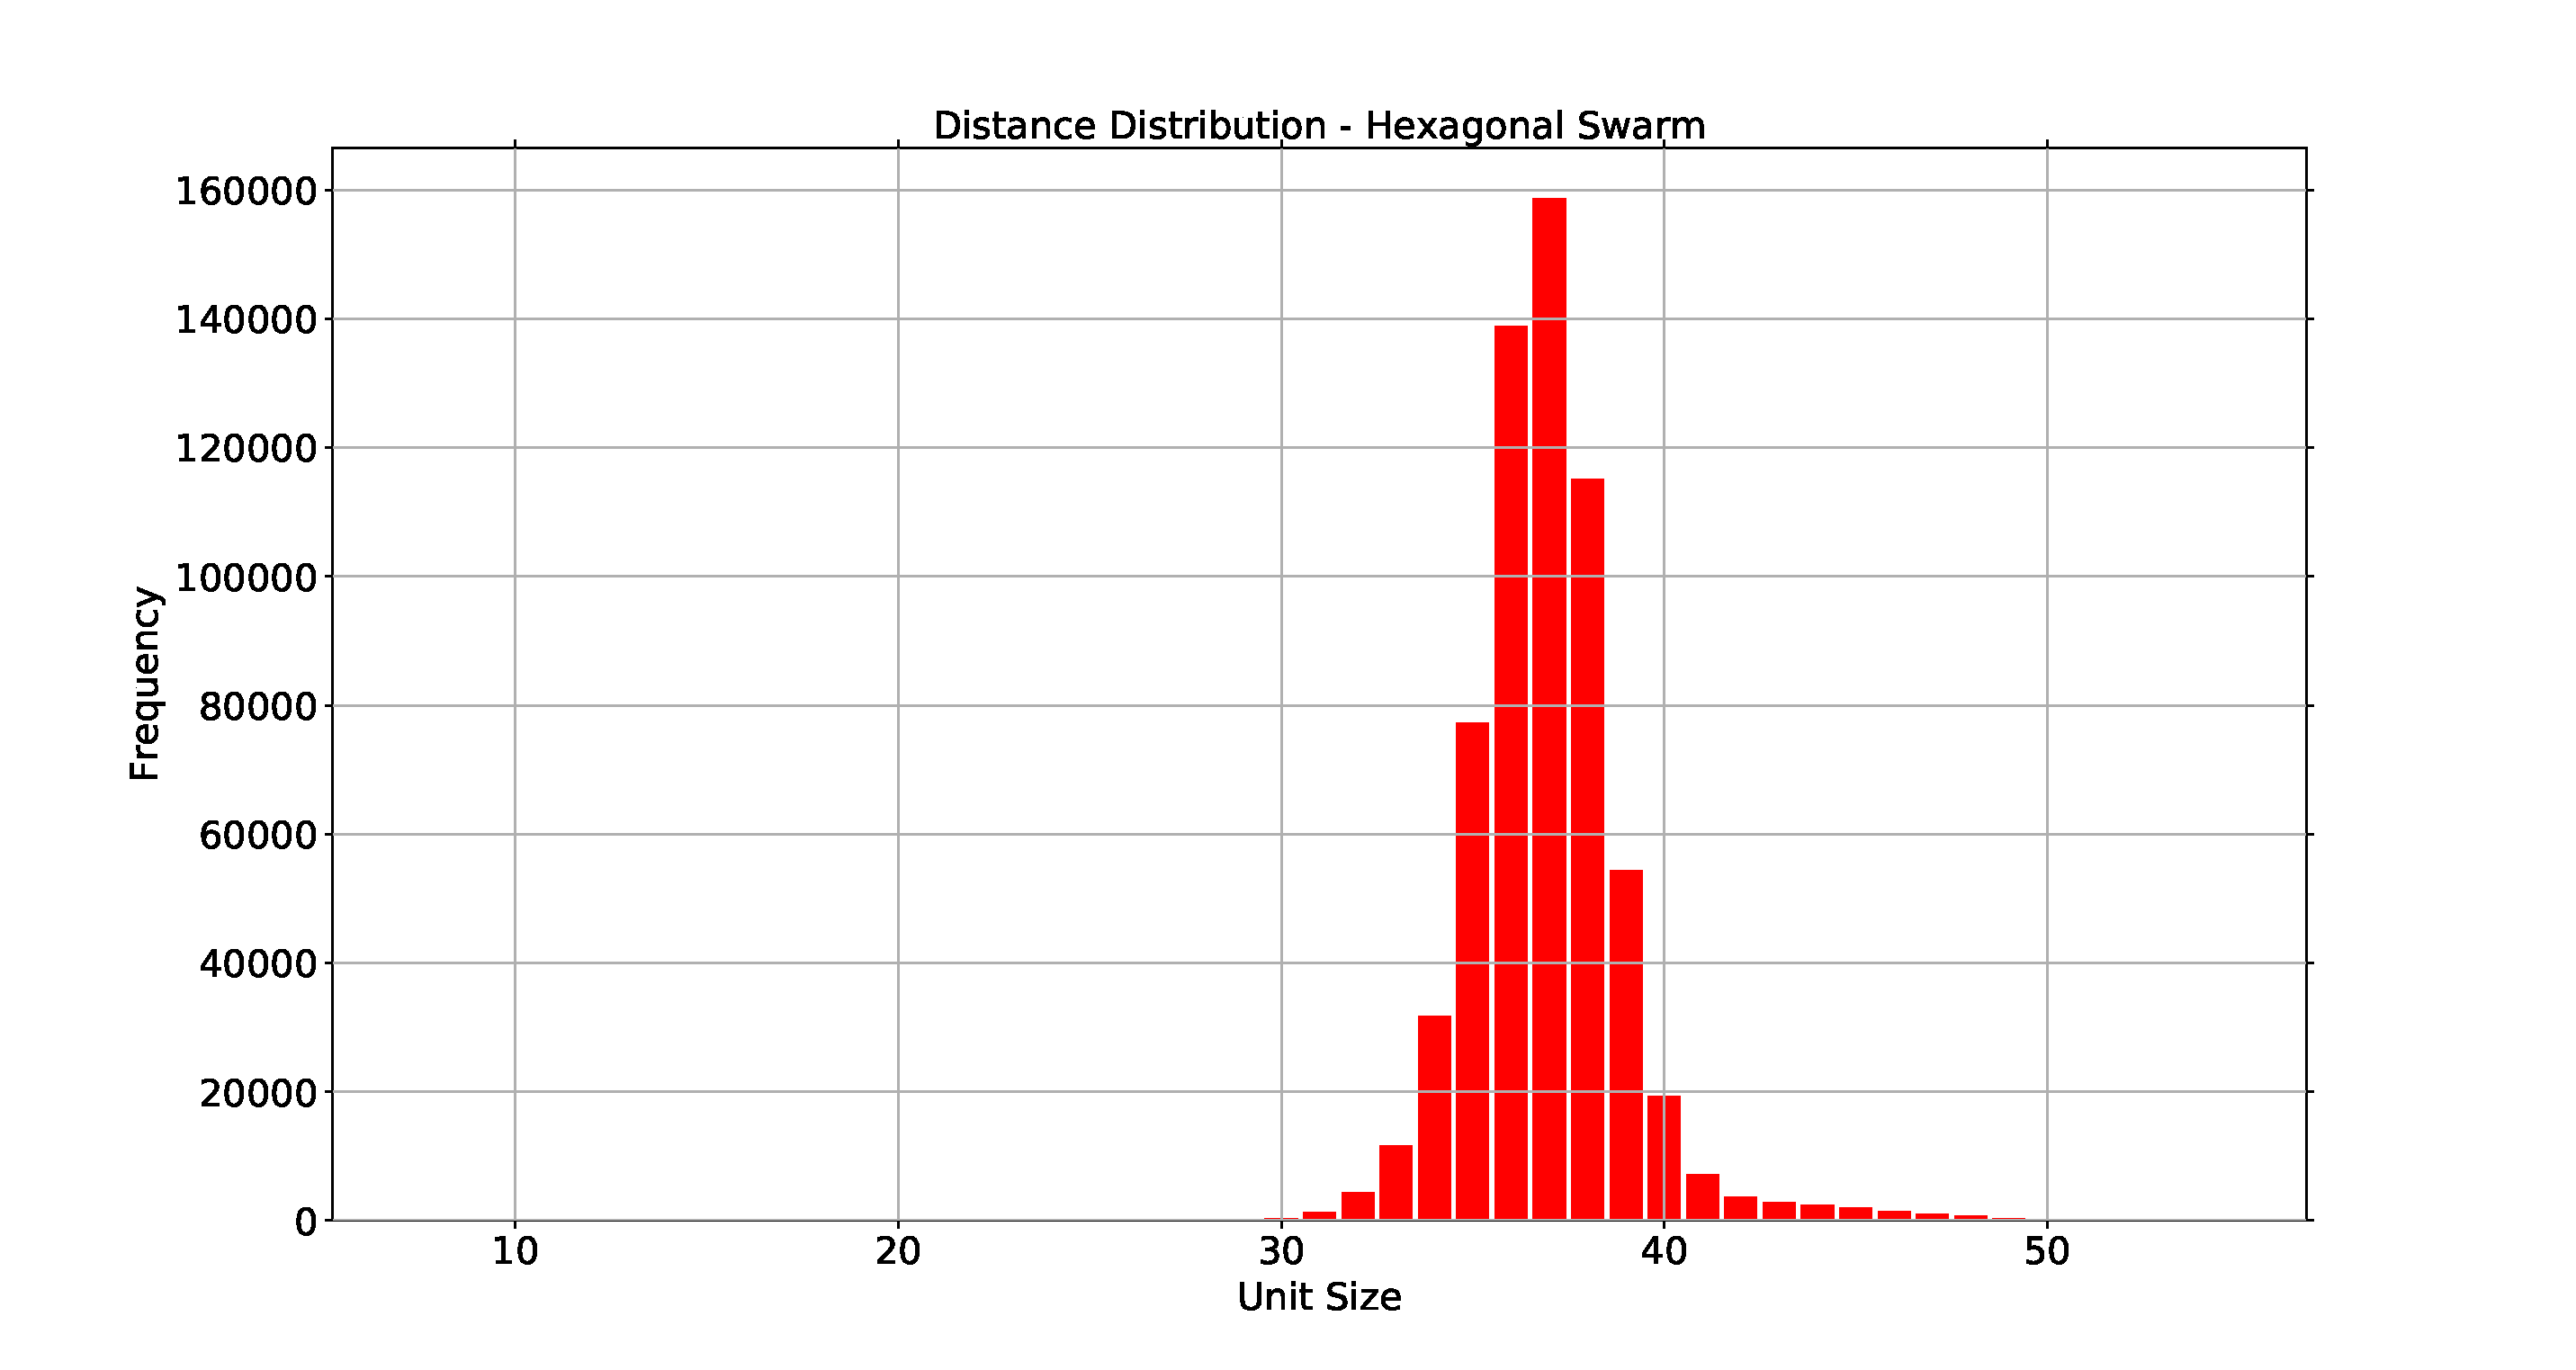
\includegraphics[width=13cm]{CHAPTER-5/figures/StabilityDistibutionHexagonal}
\end{center}
\caption{Distance distribution\label{methods:StabilityDistributionHexagonal}}
\end{figure}

Figures~\ref{methods:StabilityDistributionHexagonal3D} and \ref{methods:StabilityDistributionHexagonal3D2} show the distributions at each time cycle and shows the changes in the distribution of the distances as the agents coalesce into a stable structure. \autoref{methods:StabilityDistributionHexagonal3D} shows the initial distribution for the time intervals from 0 to 100 cycles (10 seconds). As the cycles progress the mean increases and the standard deviation reduces as the inter-agent distances equalise. \autoref{methods:StabilityDistributionHexagonal3D2} shows the final state of the swarm after 10 seconds.
%HEX-DIST-BAR-3D.py
\begin{figure}[H]
%\begin{center}
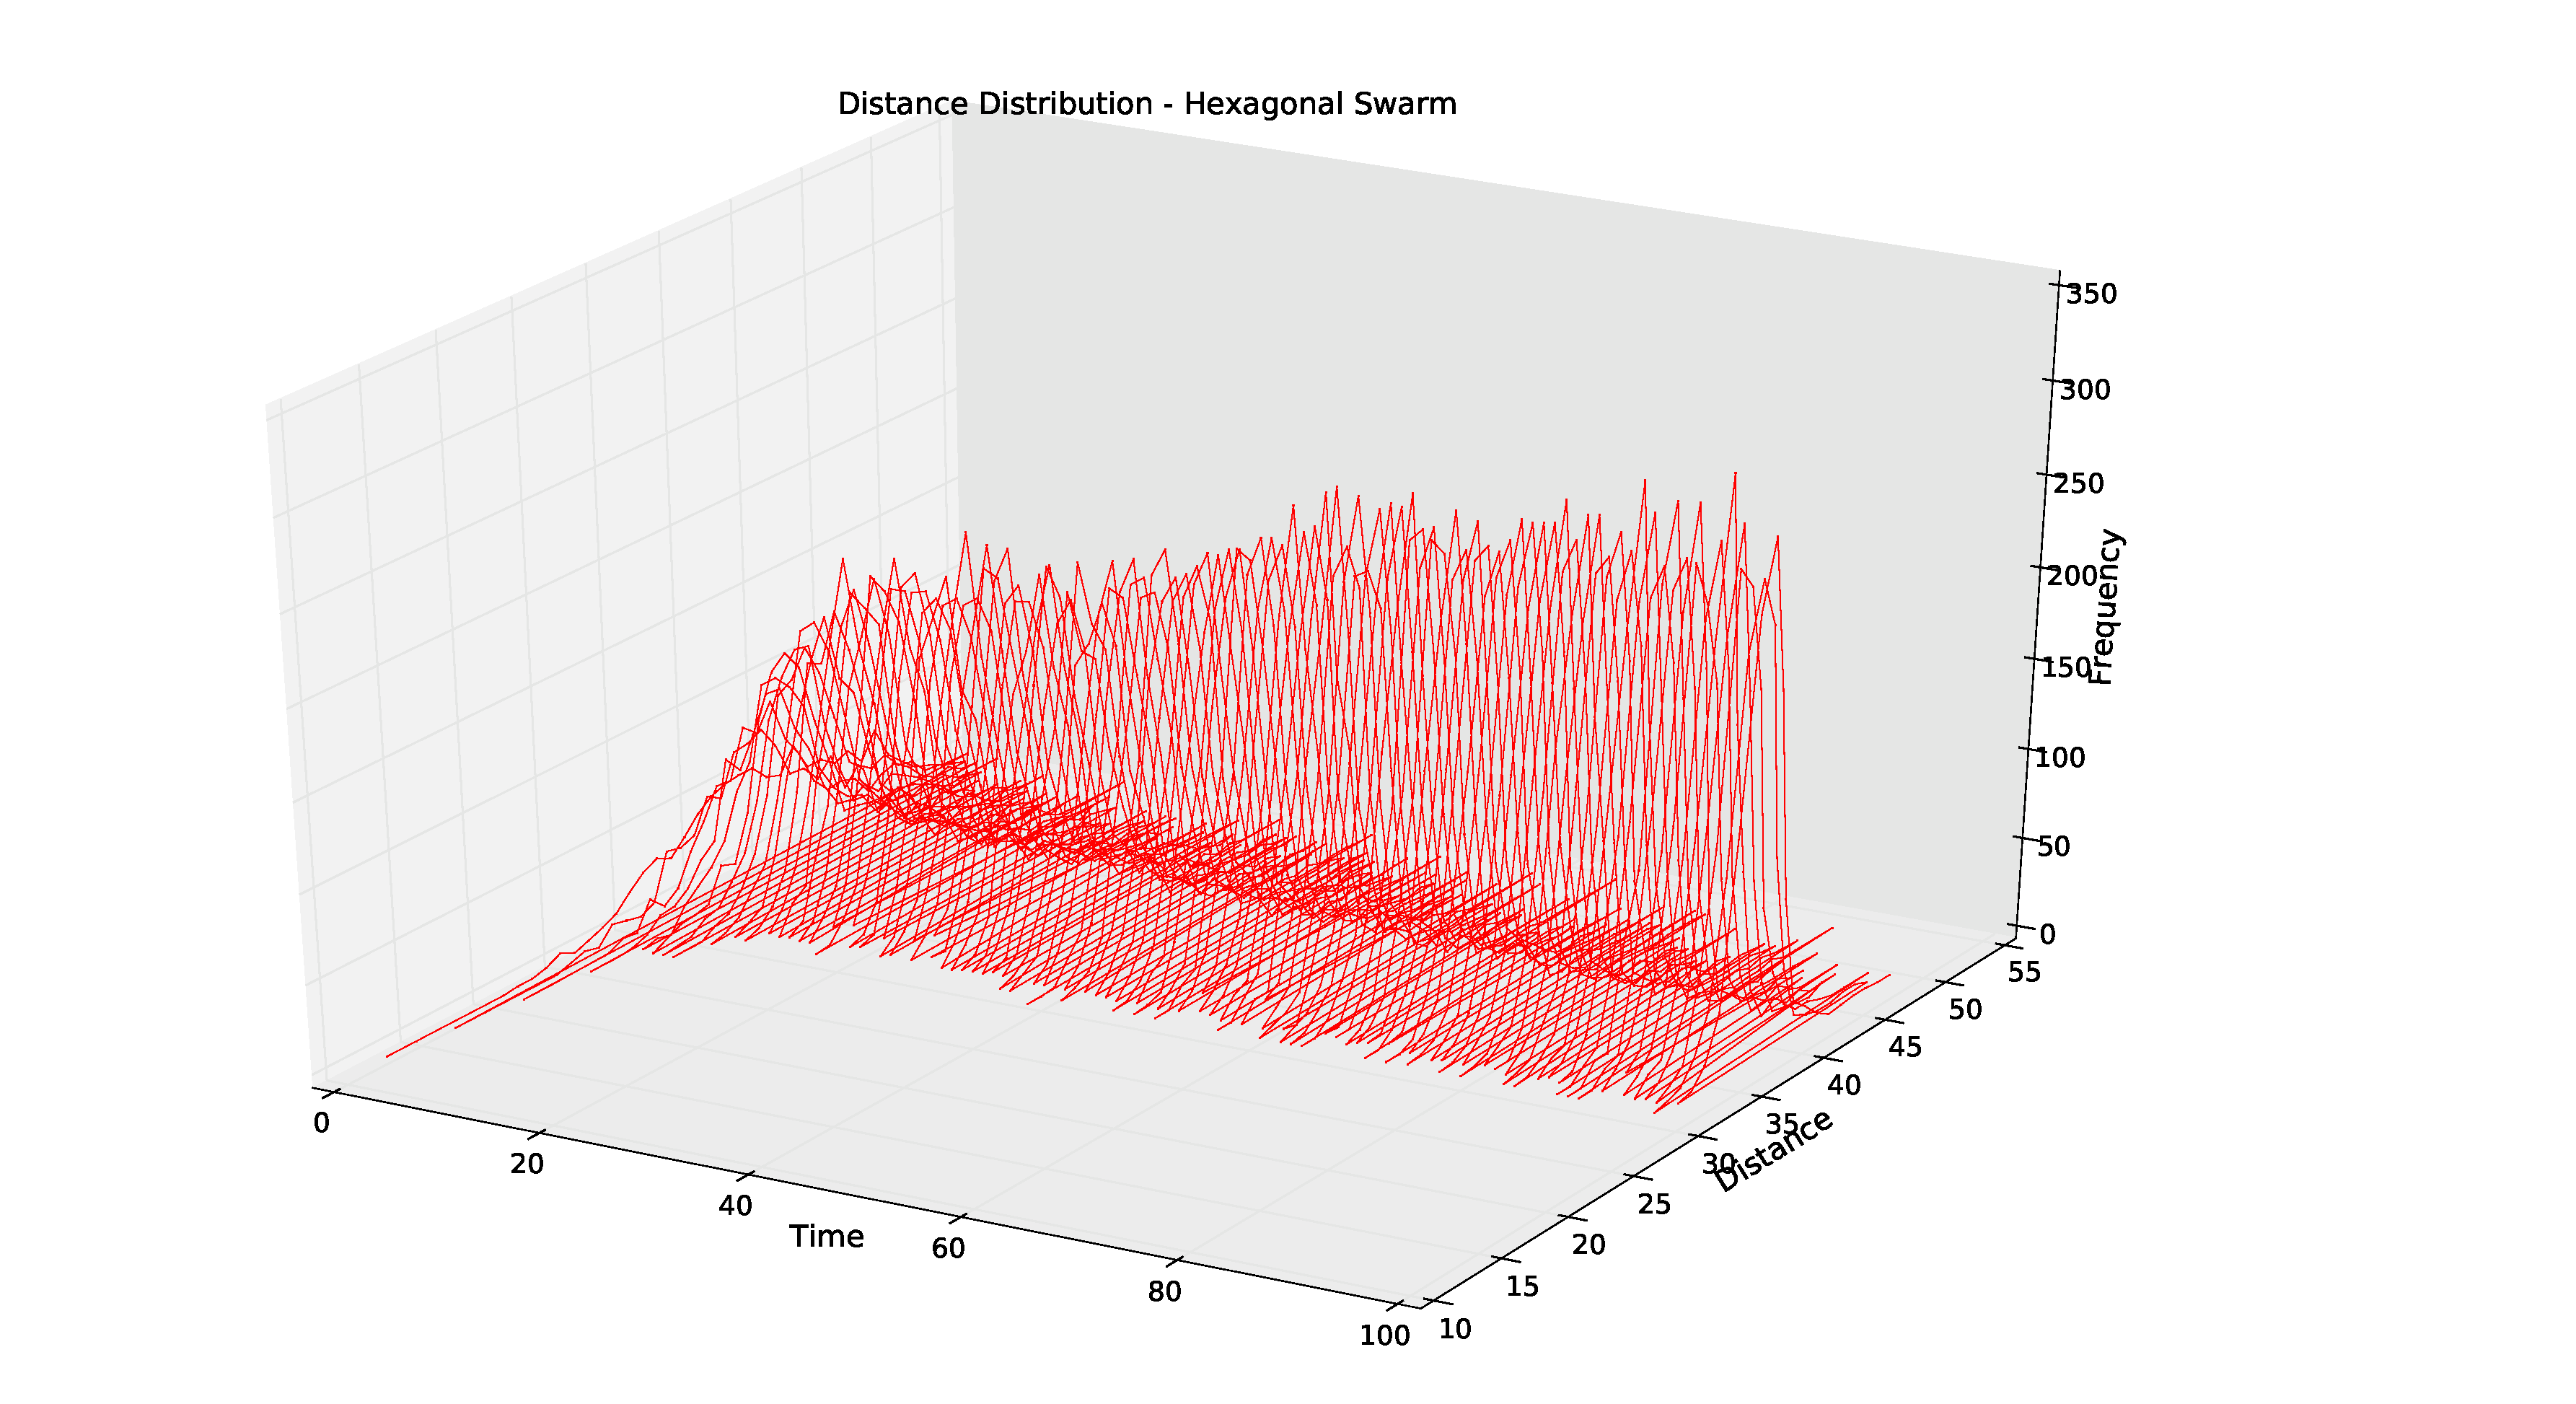
\includegraphics[width=15cm]{CHAPTER-5/figures/StabilityDistibutionHexagonal3D}
%\end{center}
\caption{Distance distribution / Time 0-10 seconds\label{methods:StabilityDistributionHexagonal3D}}
\end{figure}

\begin{figure}[H]
%\begin{center}
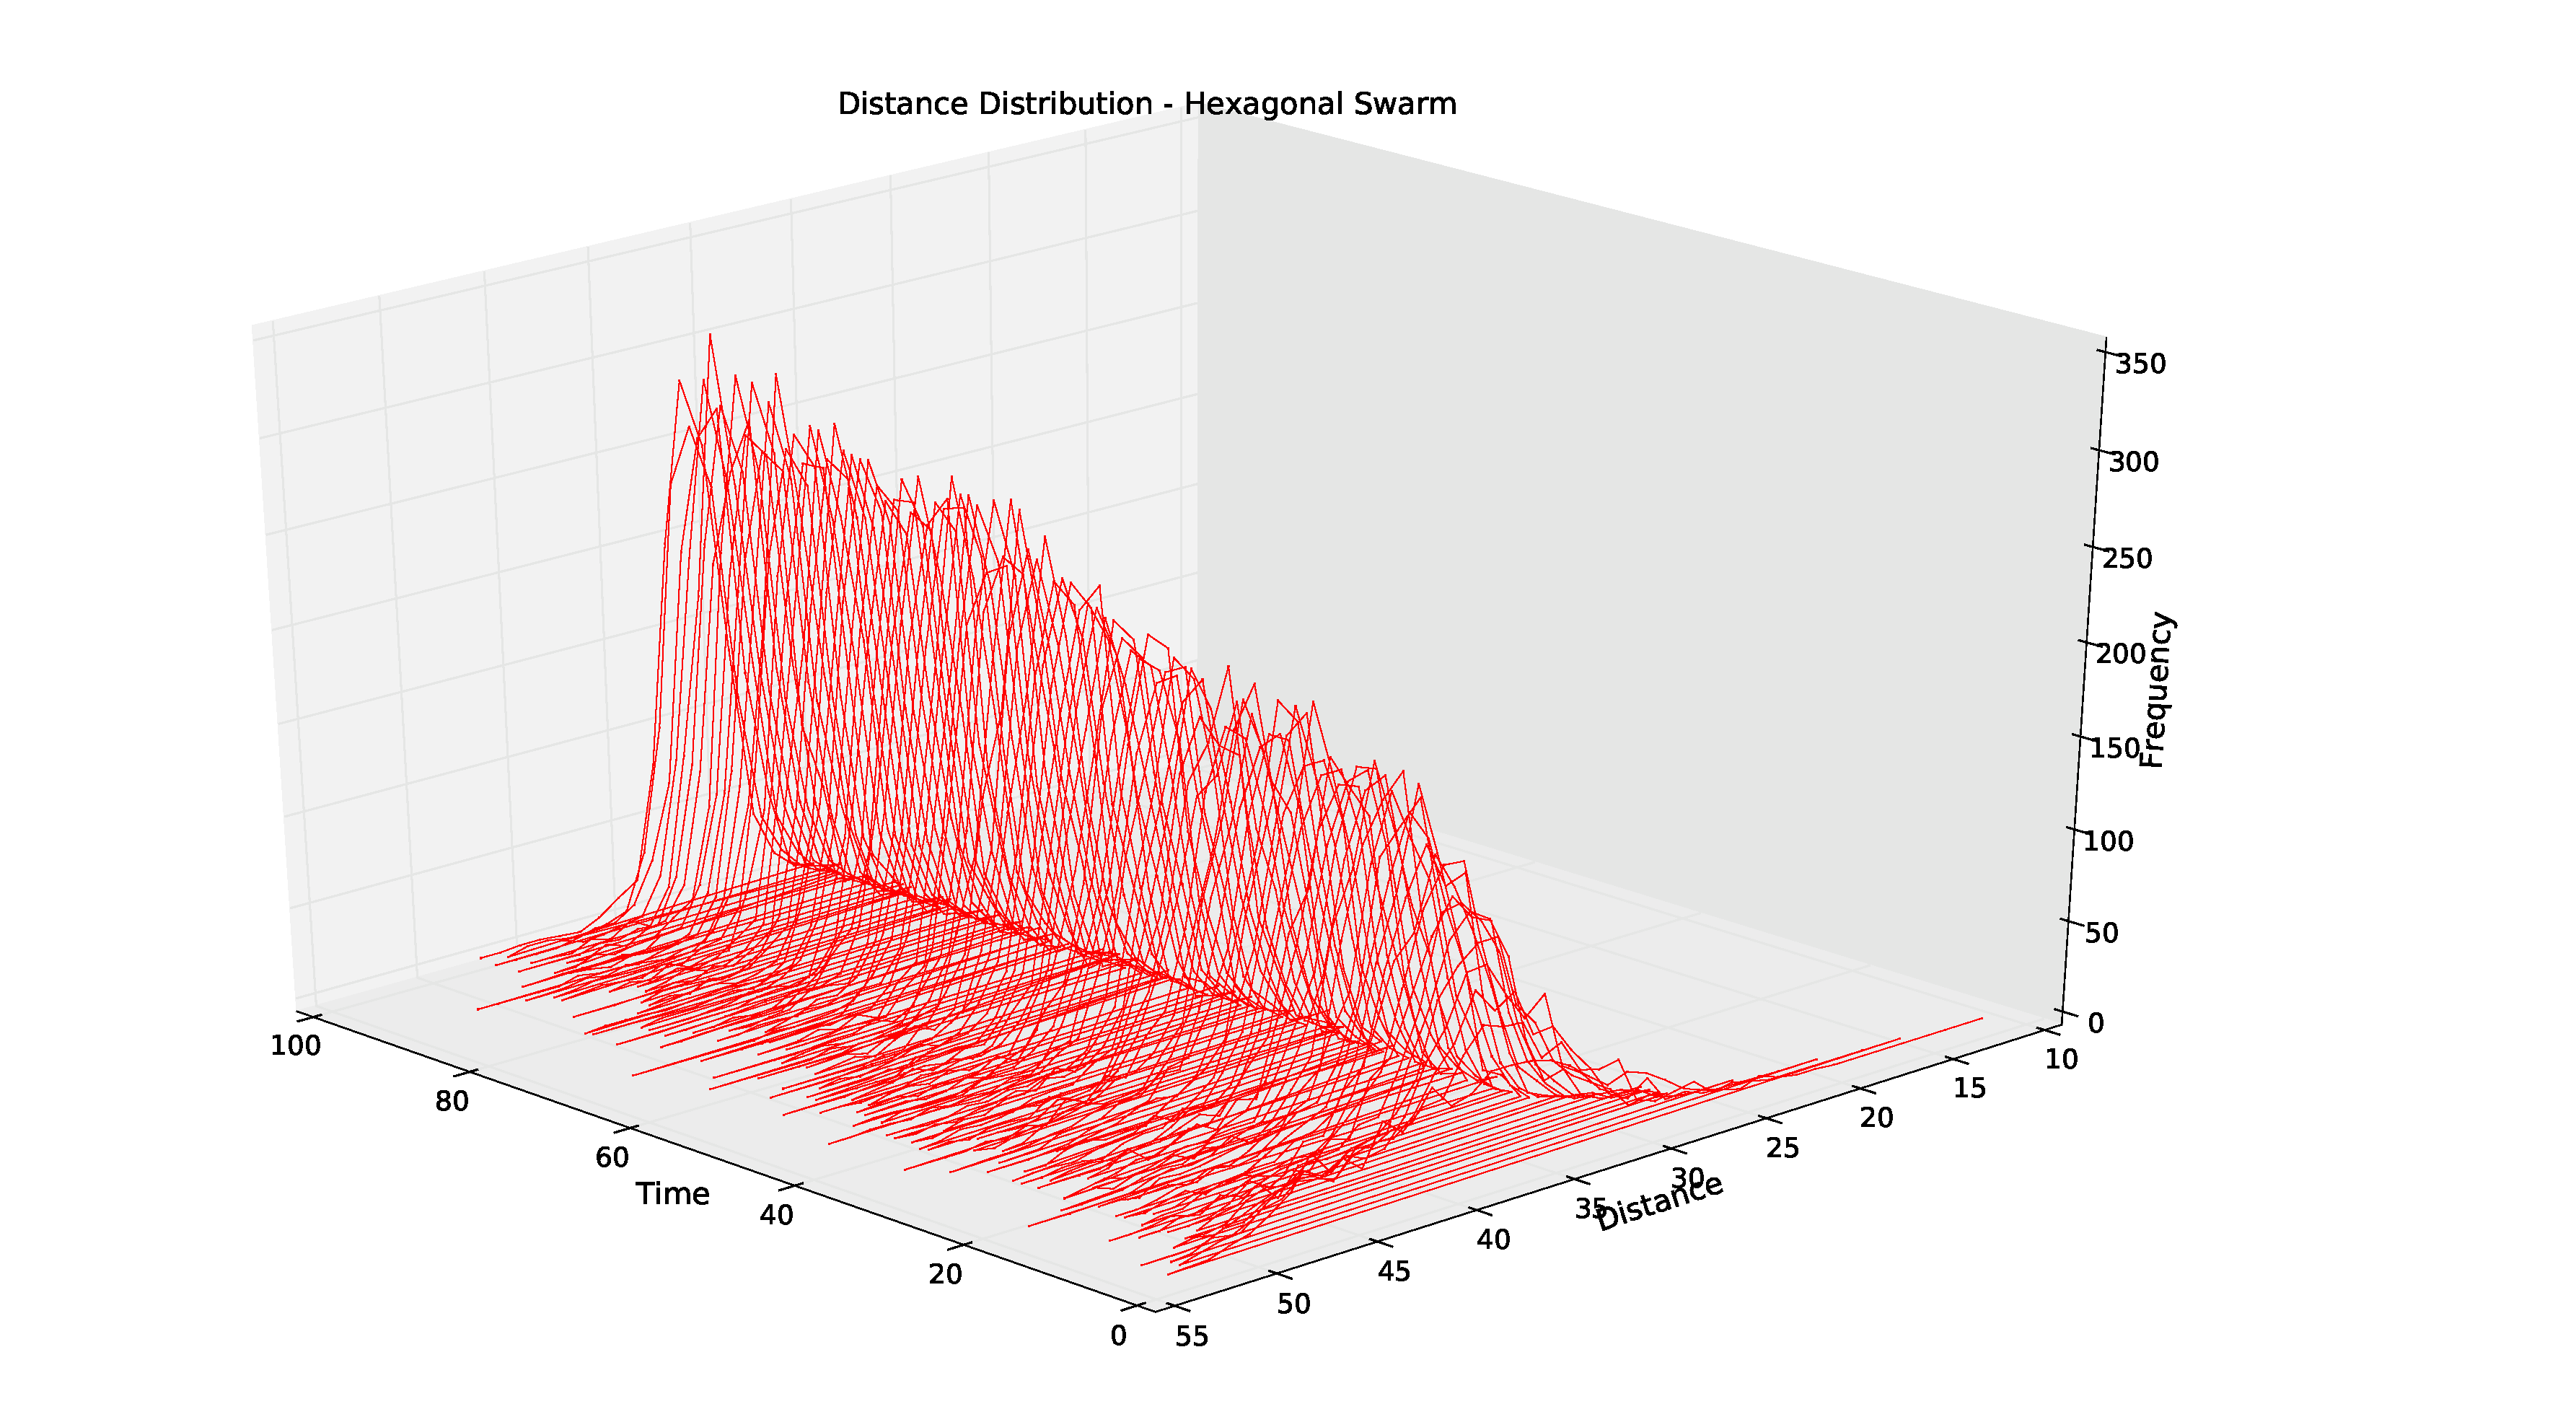
\includegraphics[width=15cm]{CHAPTER-5/figures/StabilityDistibutionHexagonal3D2}
%\end{center}
\caption{Distance distribution / Time 10-0 seconds\label{methods:StabilityDistributionHexagonal3D2}}
\end{figure}

\subsection[Agent resultant magnitude based metric]{Agent resultant magnitude (\textit{interaction vector}) based metric}
The distribution of the \textit{interaction vector} magnitude can be plotted in the same manner as the distances. \autoref{methods:StabilityMagnitudeHexagonal} shows the distribution of the agents based on the \textit{interaction vector} magnitude for the entire duration of the simulation. As with the distance based metric the data forms a normal bell shaped distribution with a mean magnitude evolving in time as shown in \autoref{methods:StabilityMagnitudeSwarm40-50}. \autoref{methods:StabilityMagnitudeHexagonal} includes negative magnitudes, this indicates that sections of the swarm are expanding. 
%HEX-MAG.py
\begin{figure}[H]
\begin{center}
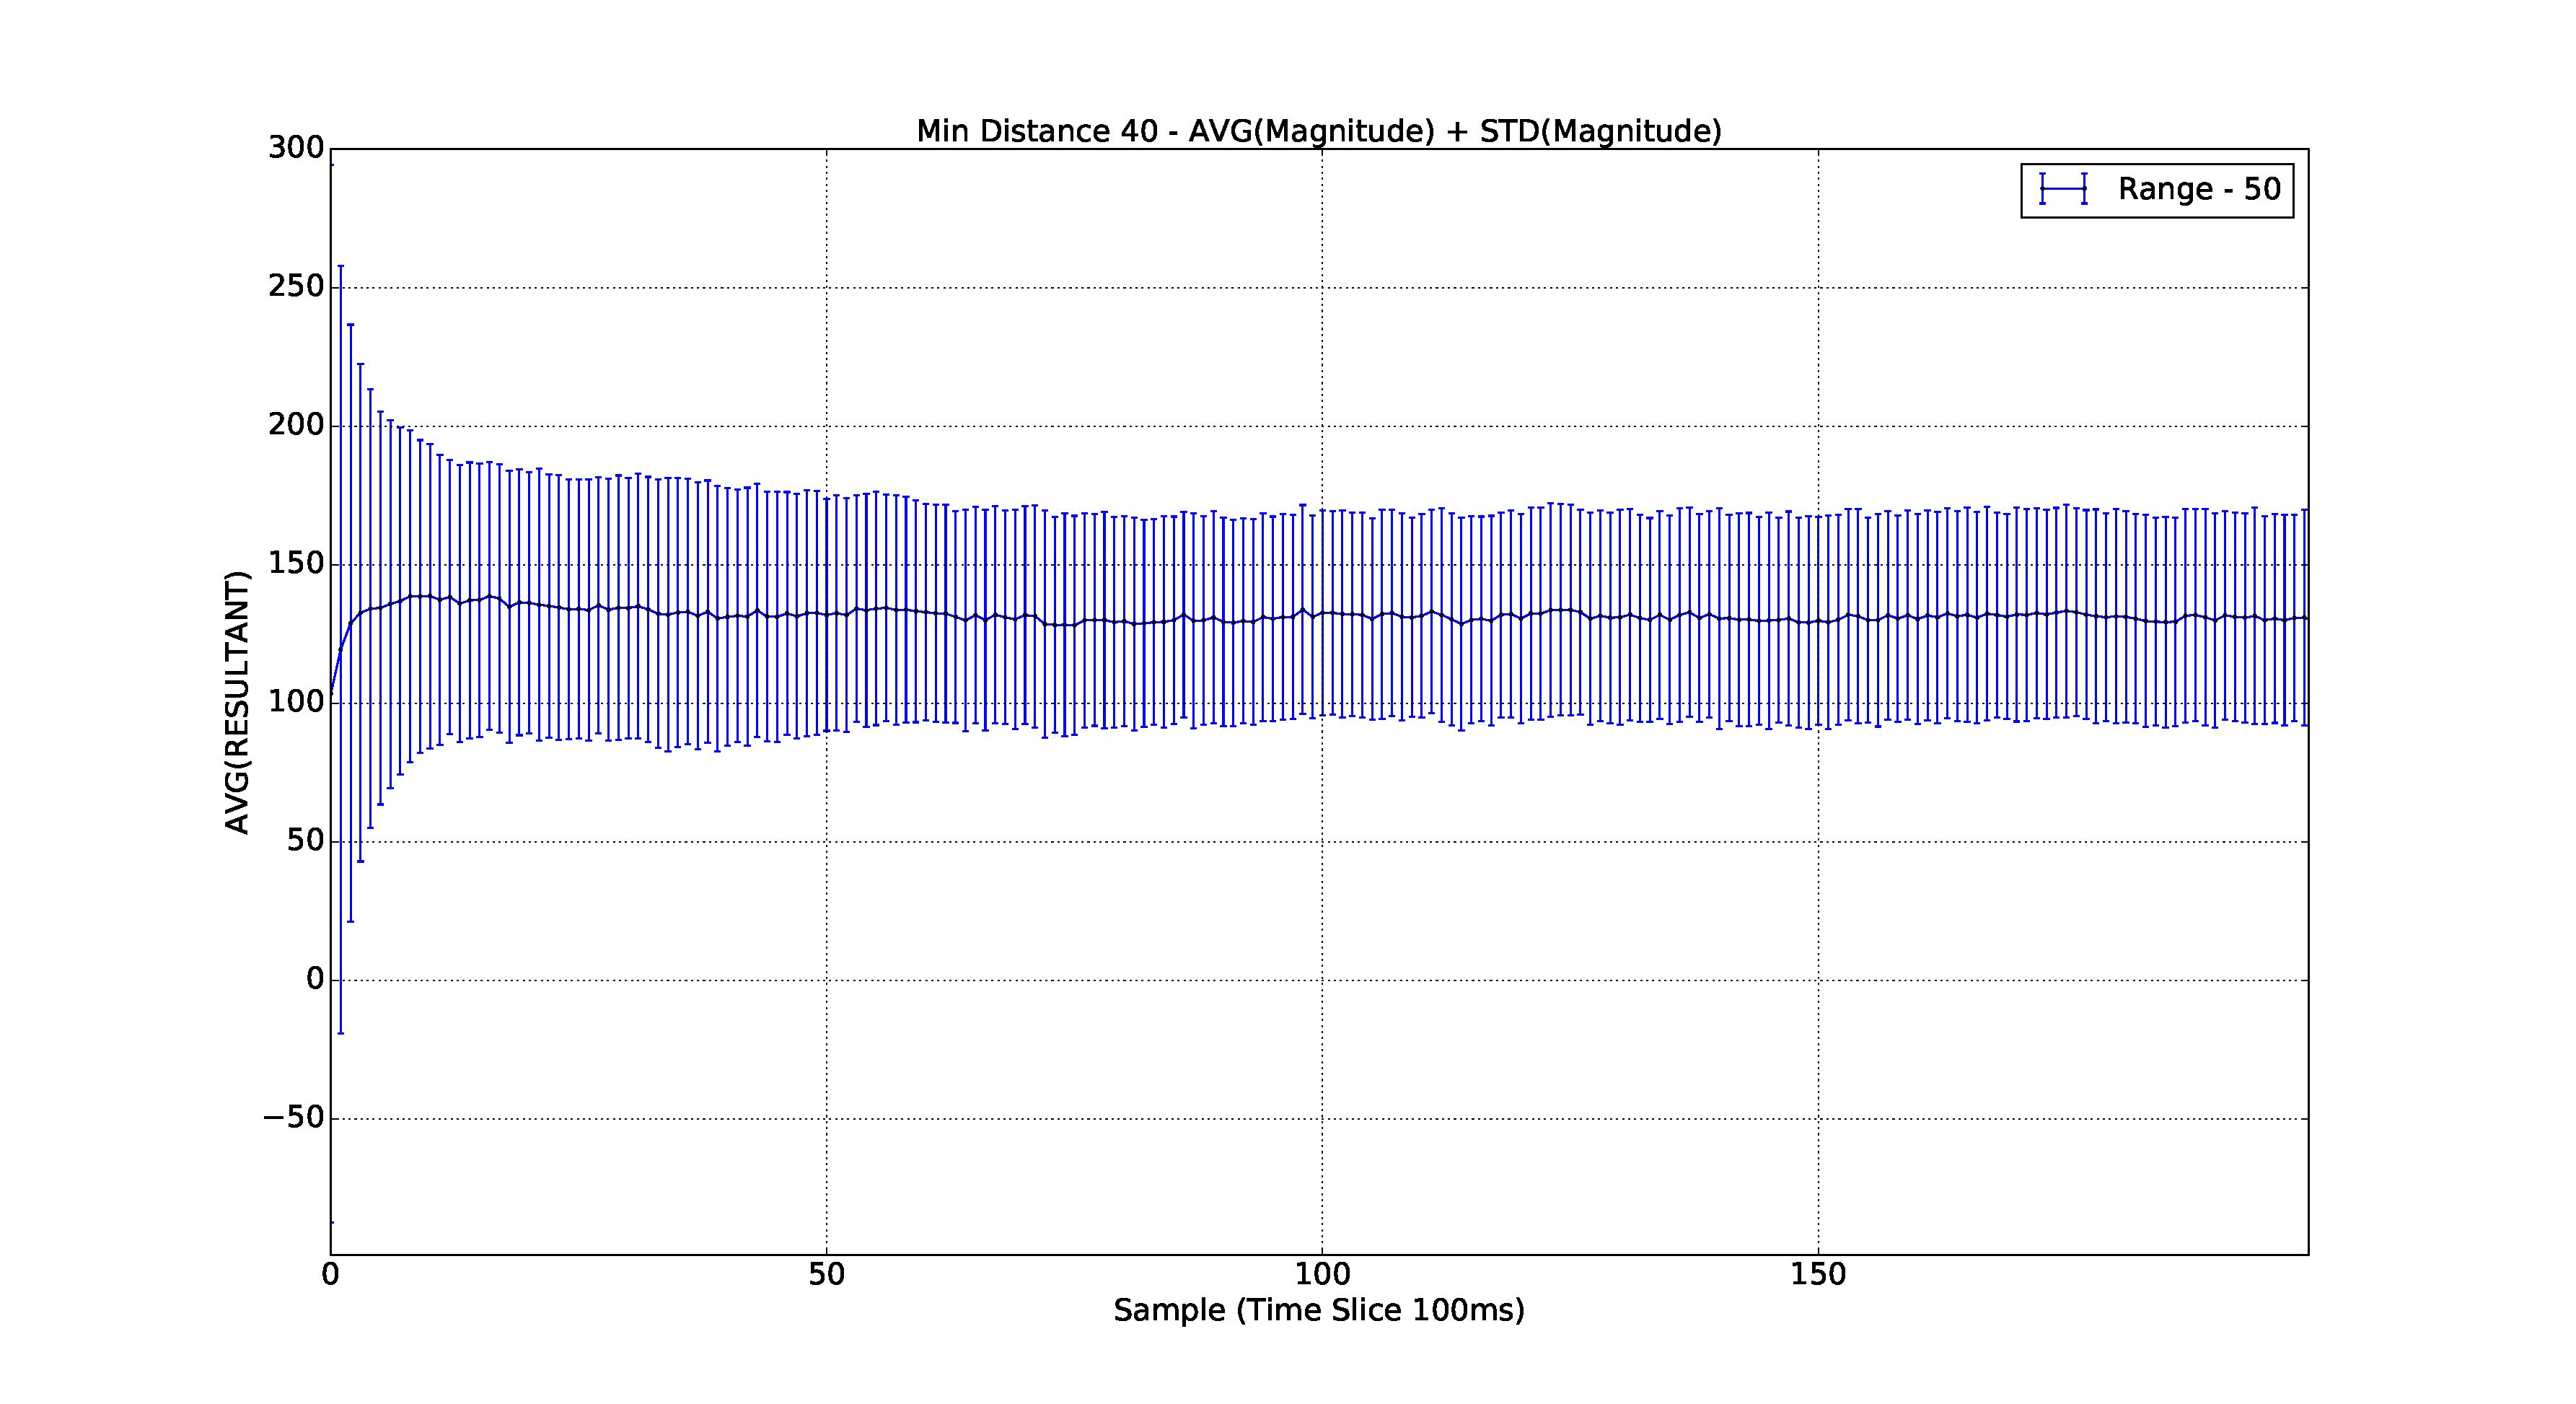
\includegraphics[width=13cm]{CHAPTER-5/figures/StabilityMagnitudeSwarm40-50}
\end{center}
\caption{Hexagonal swarm - Agent resultant magnitude metric\label{methods:StabilityMagnitudeSwarm40-50}}
\end{figure}
%HEX-MAG-BAR.py
\begin{figure}[H]
\begin{center}
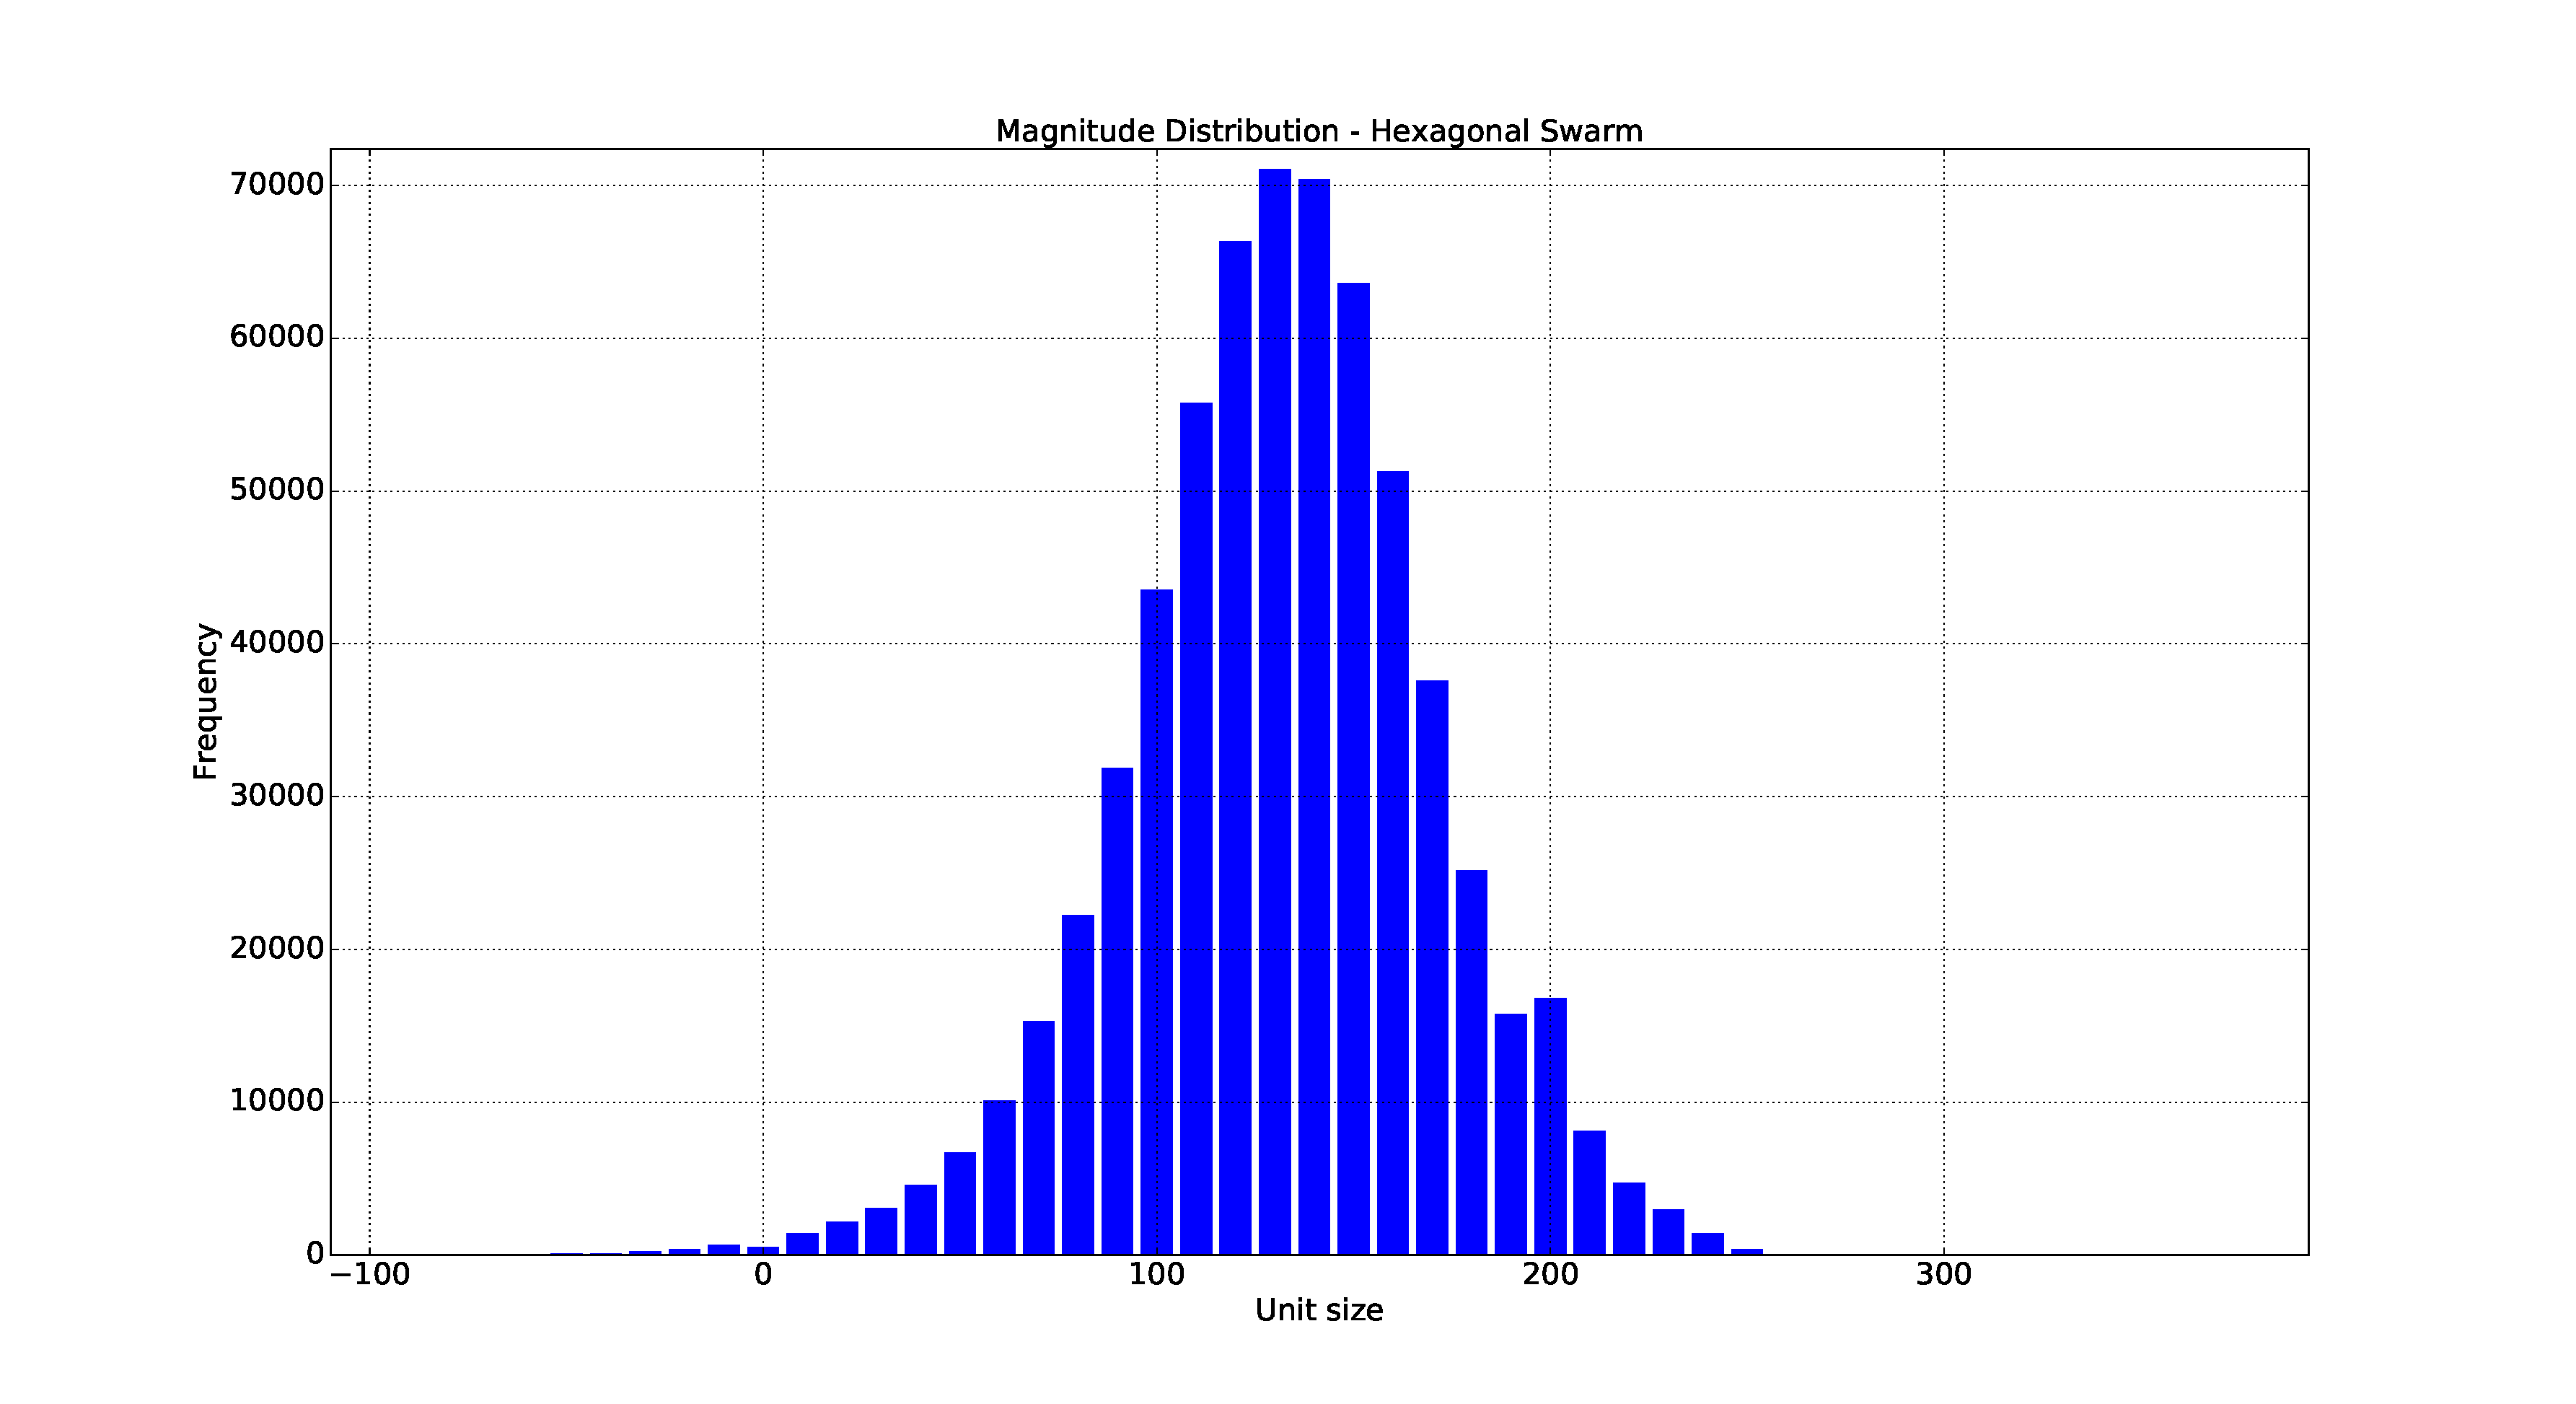
\includegraphics[width=13cm]{CHAPTER-5/figures/StabilityMagnitudeHexagonal}
\end{center}
\caption{Agent resultant magnitude distribution\label{methods:StabilityMagnitudeHexagonal}}
\end{figure}

\autoref{methods:StabilityMagHexagonal3D} and \ref{methods:StabilityDistributionHexagonal3D2} show the distributions at each time cycle and show the change in the distributions of the magnitudes. As with the distance graphs \autoref{methods:StabilityMagHexagonal3D} shows the distribution at time interval 0 to 100 and \autoref{methods:StabilityMagHexagonal3D2} shows the final state of the swarm after 10 seconds (100 cycles).

\begin{figure}[H]
\begin{center}
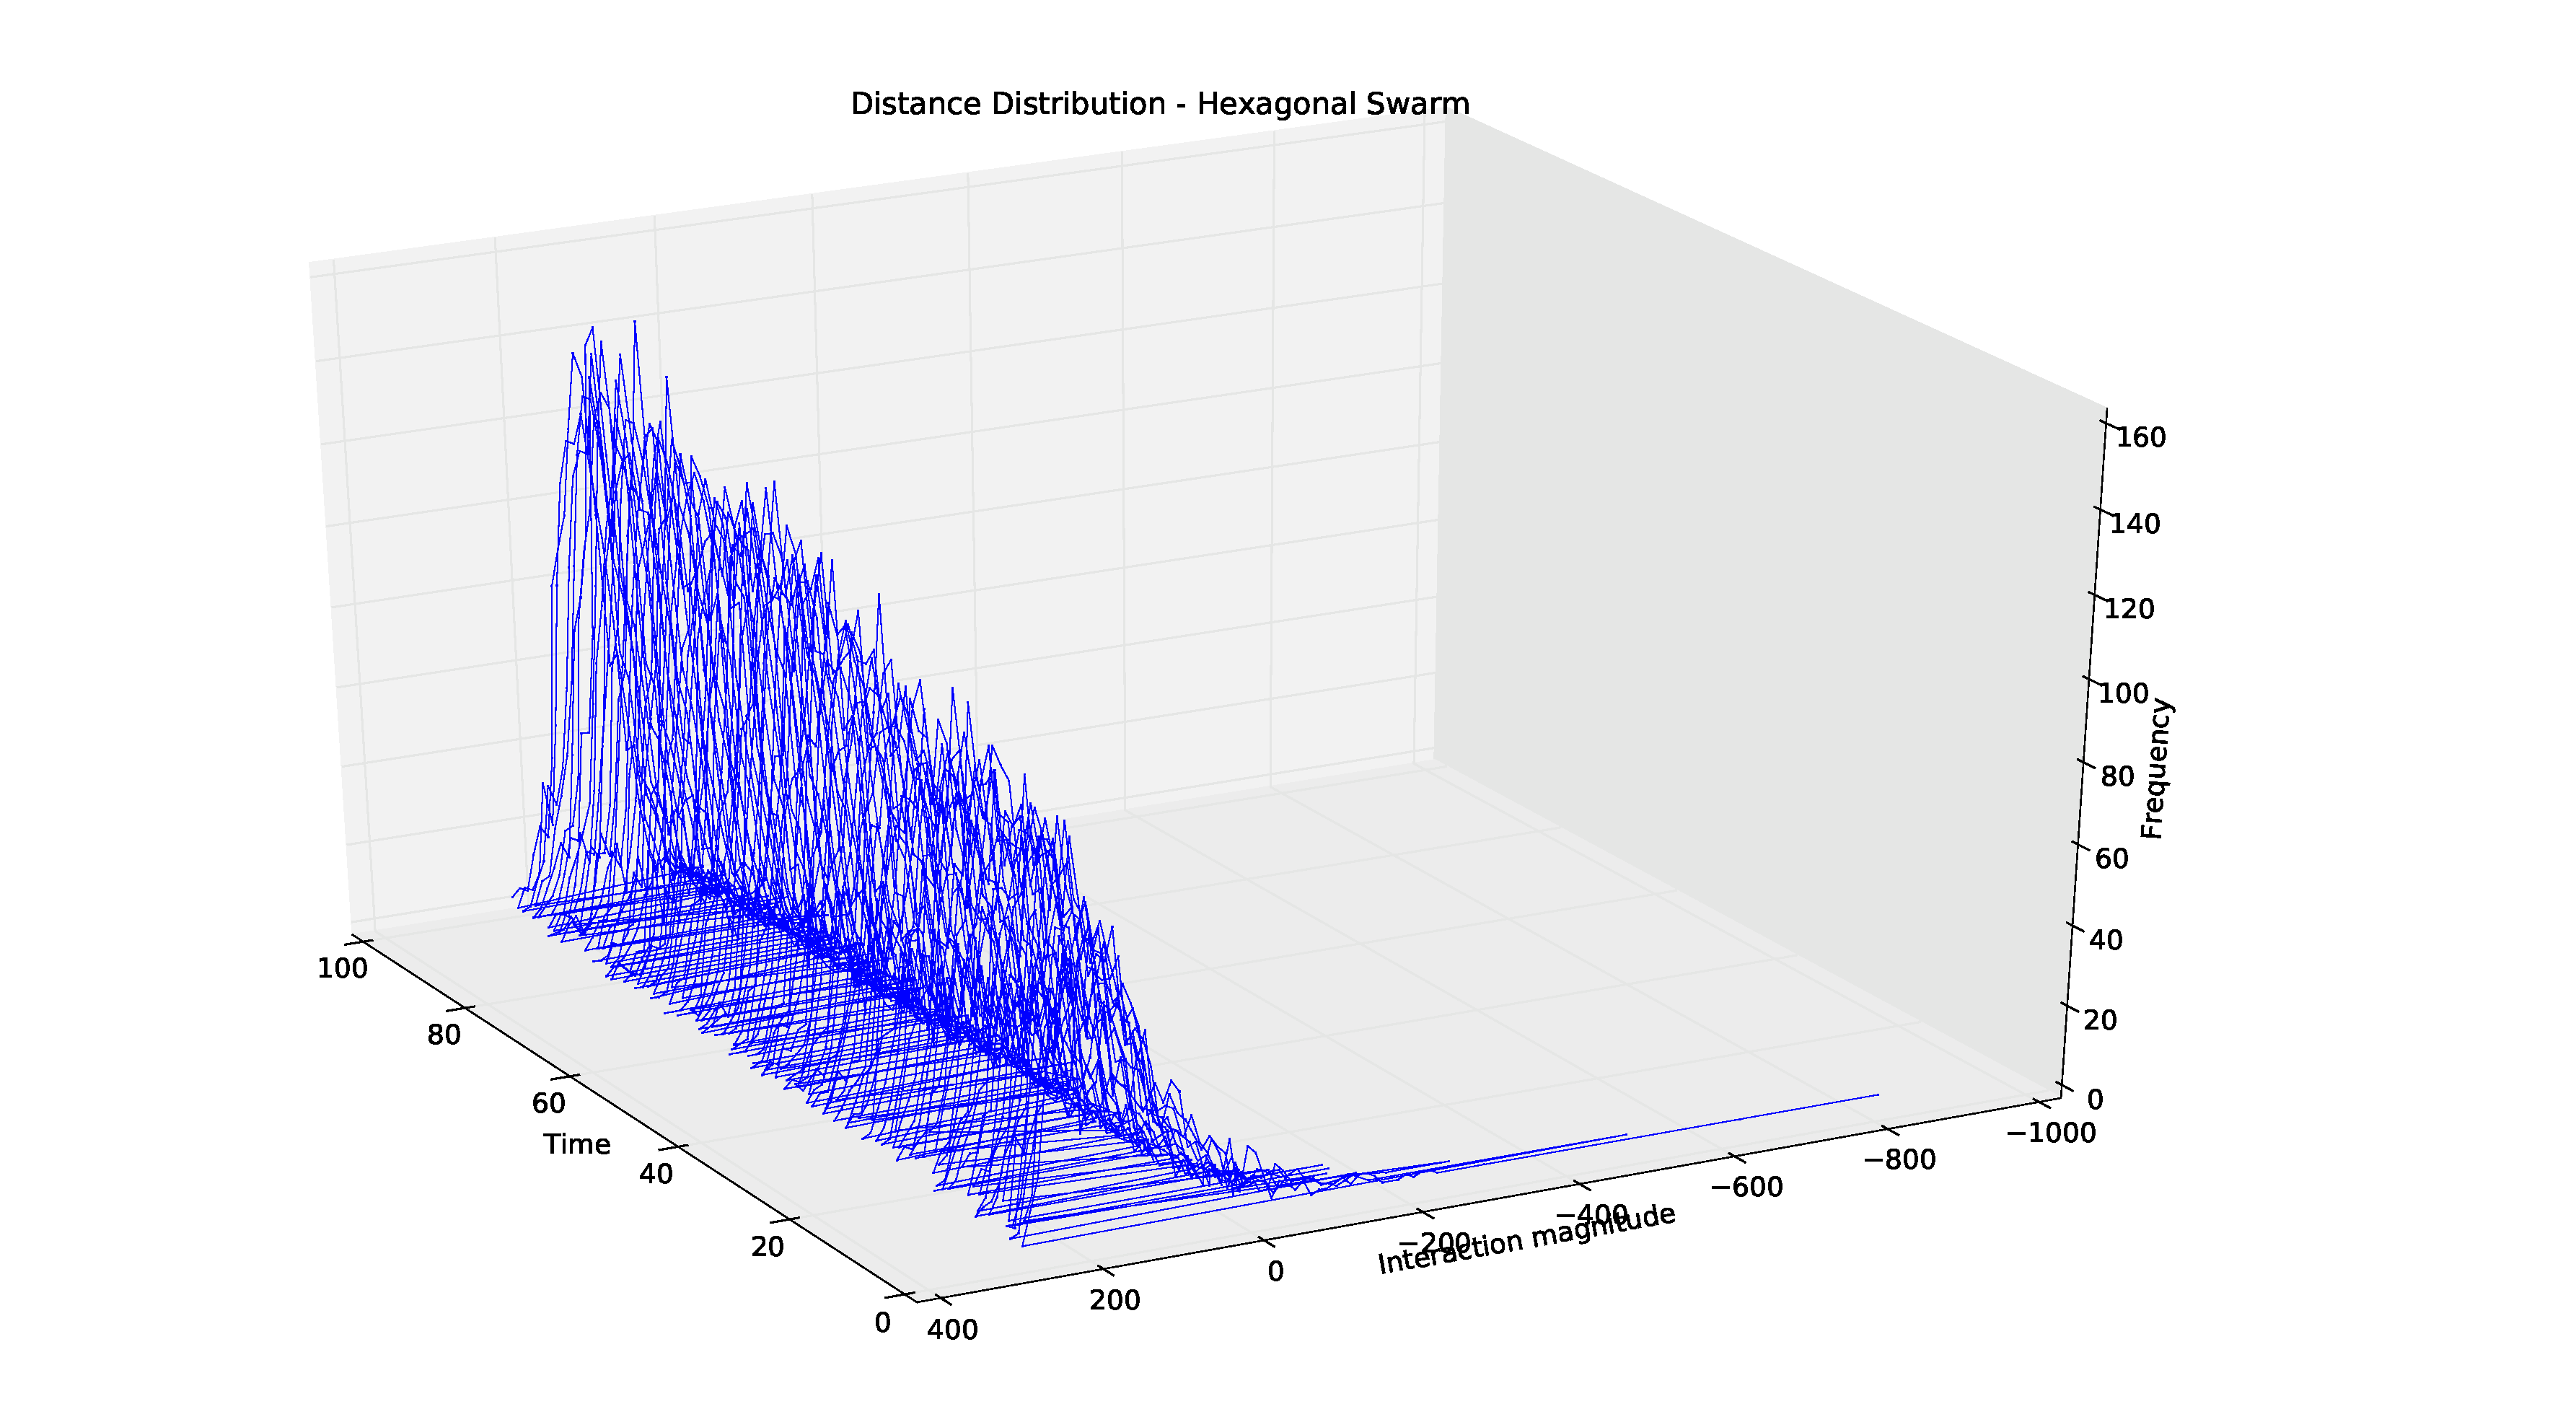
\includegraphics[width=13cm]{CHAPTER-5/figures/StabilityMagHexagonal3D}
\end{center}
\caption{Agent resultant magnitude distribution / Time 0-10 seconds\label{methods:StabilityMagHexagonal3D}}
\end{figure}

\begin{figure}[H]
\begin{center}
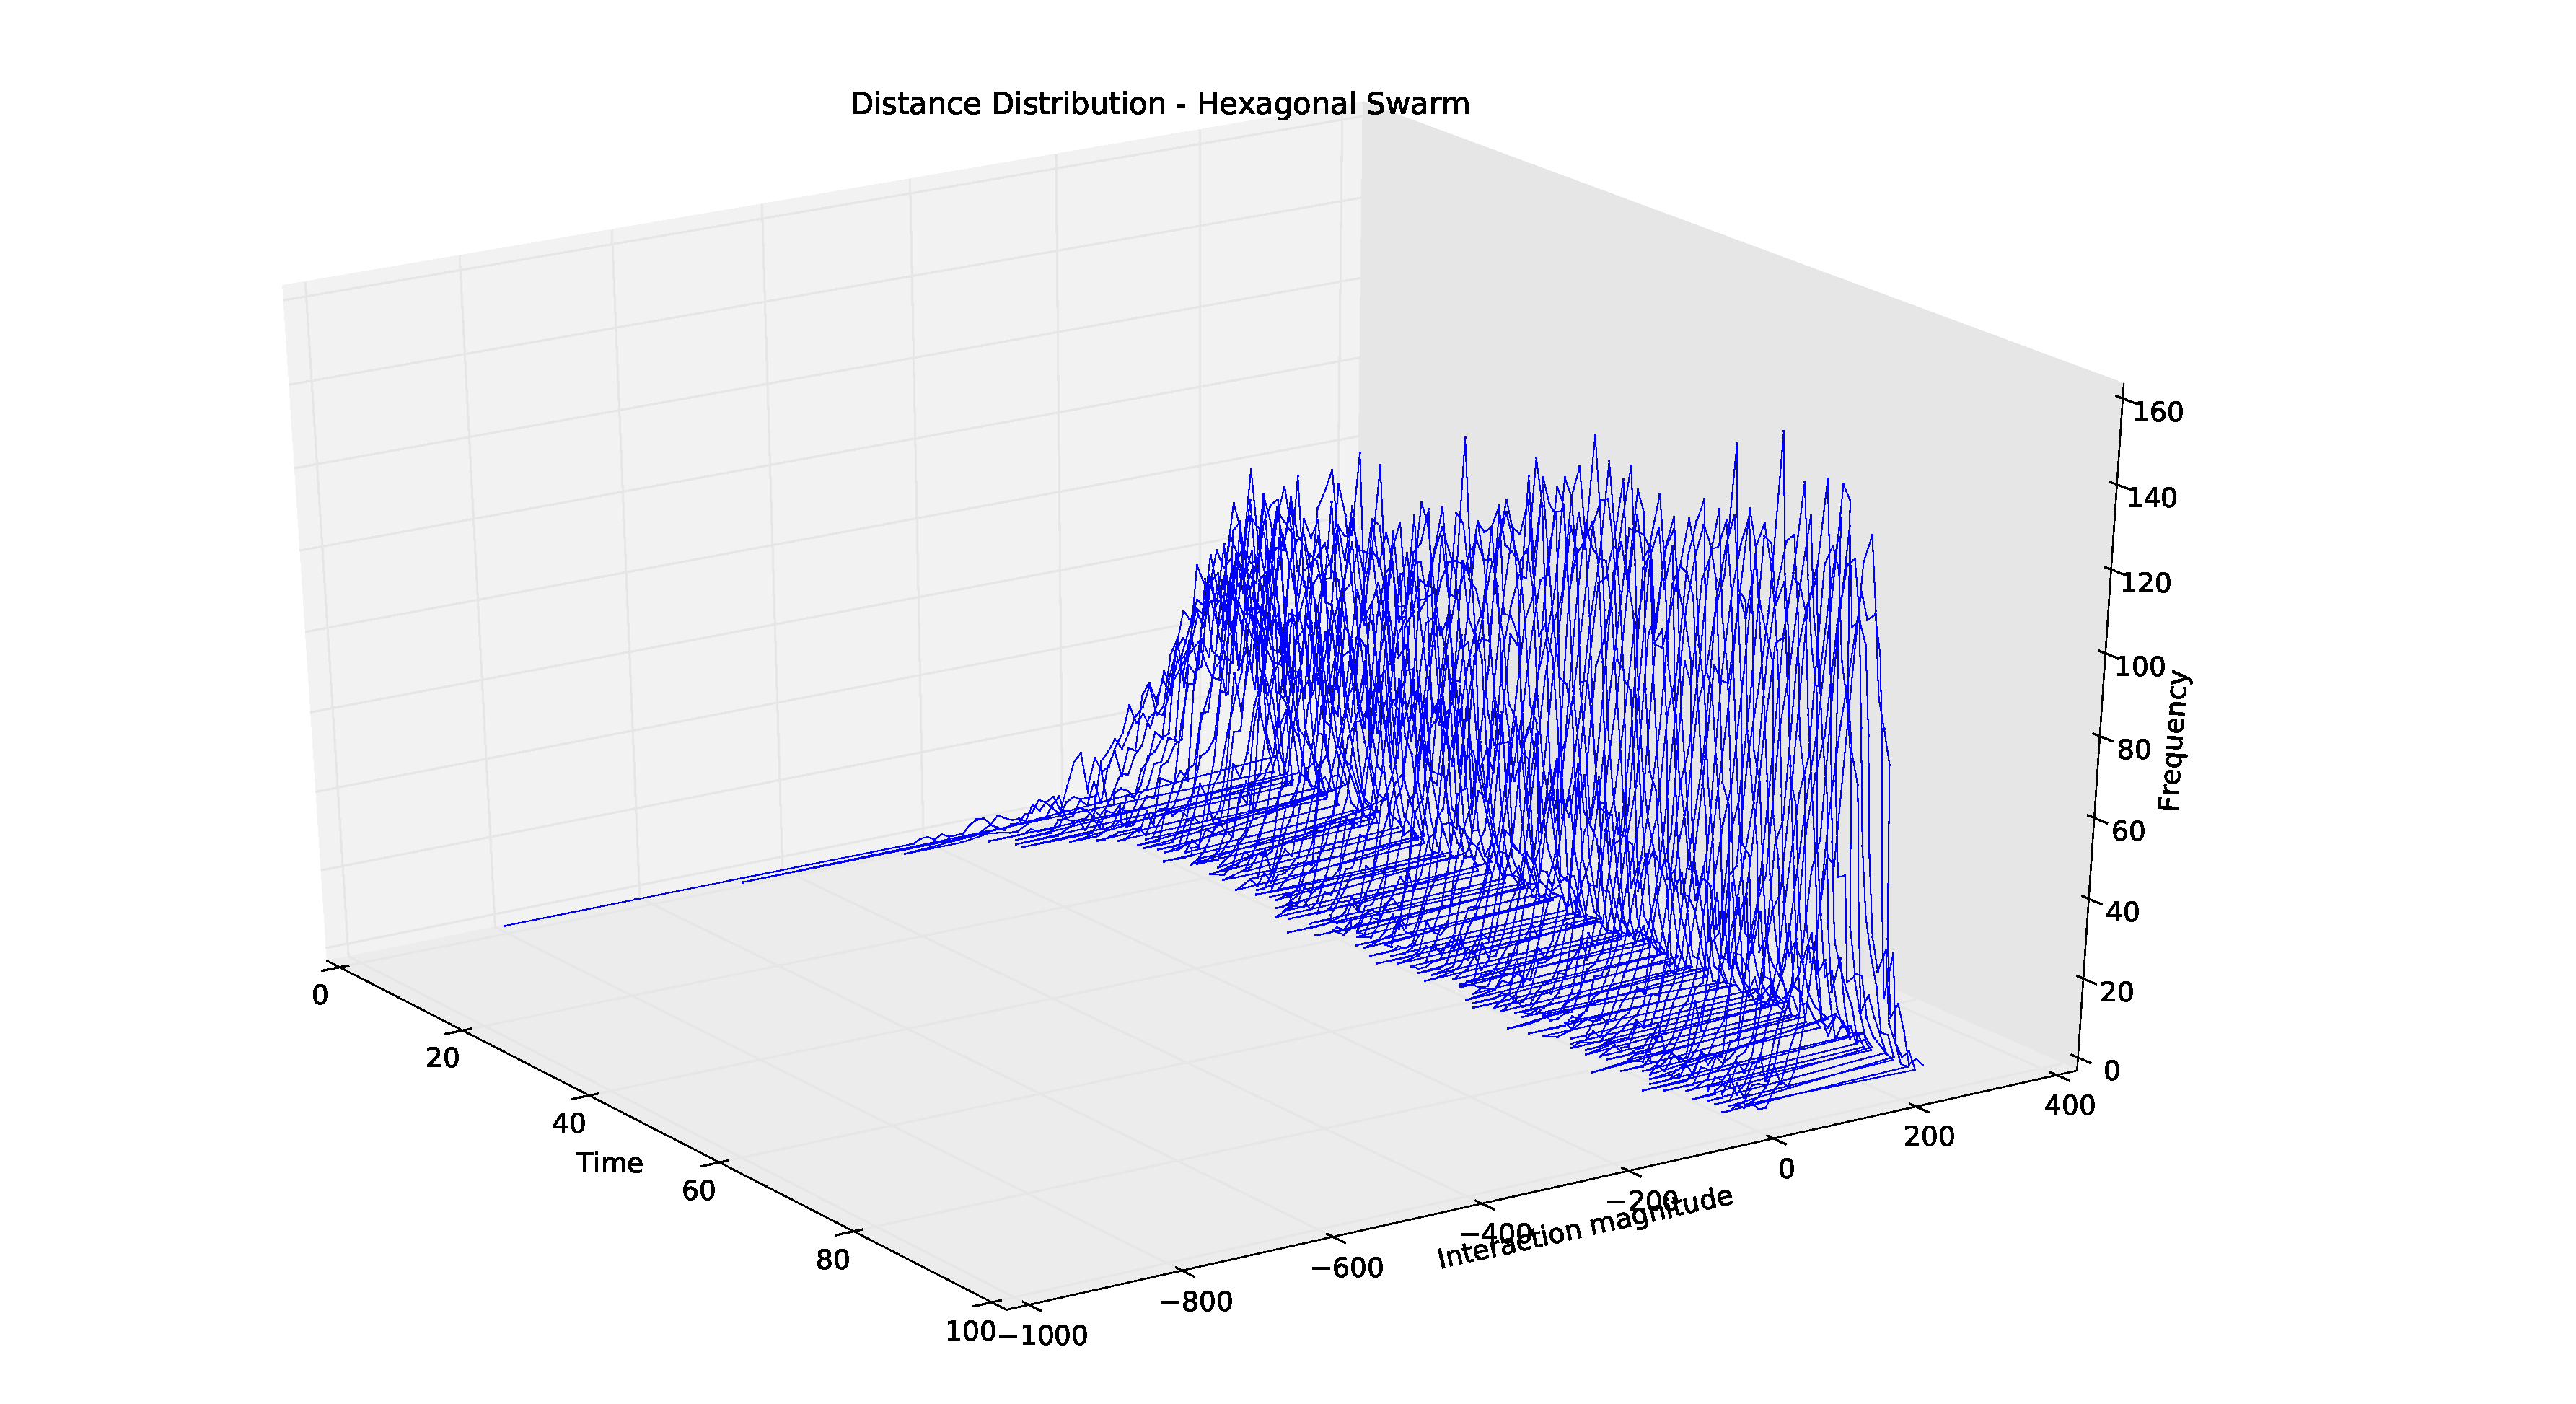
\includegraphics[width=13cm]{CHAPTER-5/figures/StabilityMagHexagonal3D2}
\end{center}
\caption{Agent resultant magnitude distribution / Time 10-0 seconds\label{methods:StabilityMagHexagonal3D2}}
\end{figure}

The hexagonal structure is the most stable structure \cite{HT:2001} and can be classed as a swarms most efficient state as the swarm is maximally distributed with agents having minimal or no cross connected agents. These results show that the field effects are producing a swarm that will tend towards having all distances equal which will produce the hexagonal effect as shown in \autoref{fig:StableForms} on page \pageref{fig:StableForms}.

\section{Hyper-connected swarm analysis}\label{section:AnalysisB}
When the field effects create a hyper-connected swarm the inter connectivity of the agents create a multi-modal distribution of the inter-agent distances. \autoref{methods:CrushedStability1} shows the inter-agent distances highlighted, near neighbours in green and extended neighbours in red. This is detectable in terms of how the internal movement metrics present these distributions. A hyper-connected swarm has a high level of cohesion causing the swarm to become very inflexible. The swarm appears `stable' in terms how the overall structure is maintained~(\autoref{methods:StableSwarmCompressed}), however, there is a greater variation in the \textit{interaction vector} magnitudes, and resultant distances, than in a hexagonal swarm. The distances will maintain a good sound structure but the standard deviation from the mean is high. This elevated standard deviation~(\autoref{methods:StabilityDistanceSwarm40-60} and ~\ref{methods:StabilityMagnitude40-60}) indicates that the swarm is not at its optimum distribution as the swarm's agents could be distributed further covering a greater area without causing the swarm to break up. This can be achieved by increasing the repulsion field effect. In some circumstances this hyper-connected structure may be a desirable configuration to create a more `rigid' platform: for instance to provide a close proximity wireless sensor network with multiple routing pathways. The connected distribution that causes the high standard deviation can be seen in \autoref{methods:StabilityDistributionHyper}. There are two distinct peaks in the inter-agent distribution at approximately 38 and 58 units

\begin{figure}[H]
\begin{center}
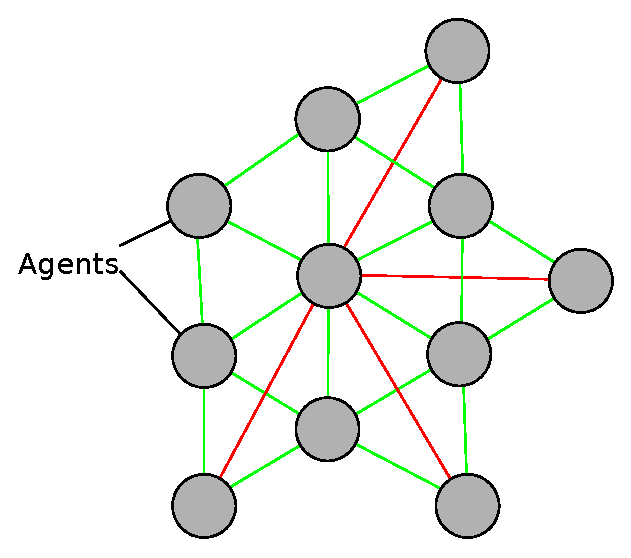
\includegraphics[width=7cm]{CHAPTER-5/figures/CrushedStability}
\end{center}
\caption{Inter-agent links in a hyper-connected swarm} \label{methods:CrushedStability1}
\end{figure}

\begin{figure}[H]
\begin{center}
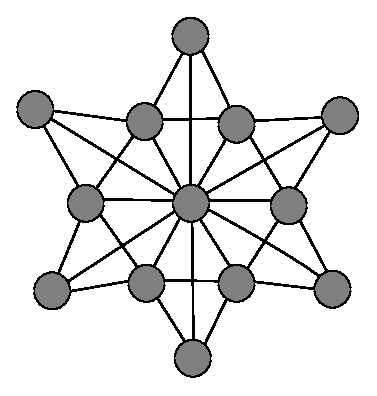
\includegraphics[width=6cm]{CHAPTER-5/figures/StableFormsCompressed}
\end{center}
\caption{Hyper-connected structure} \label{methods:StableSwarmCompressed}
\end{figure}

\subsection{Distance based metric}
The distance based analysis graph~(\autoref{methods:StabilityDistanceSwarm40-60}) for the hyper-connected swarm shows the metrics being applied to the swarm over a period of 200 cycles. 

The swarm is initially in a state of disorganisation and the average distance over the first 20 cycles shows the swarm compressing as the average distance falls. The swarm then enters a phase where the mesh structure forms and the swarm starts to stabilise. After about 100 cycles the field effects have resolved and the swarm structure settles to its most stable state for the given set of parameters. As with the hexagonal swarm the hyper-connected swarm's internal movement fluctuates to maintain the swarm's structure.
%HYPER.py
\begin{figure}[H]
\begin{center}
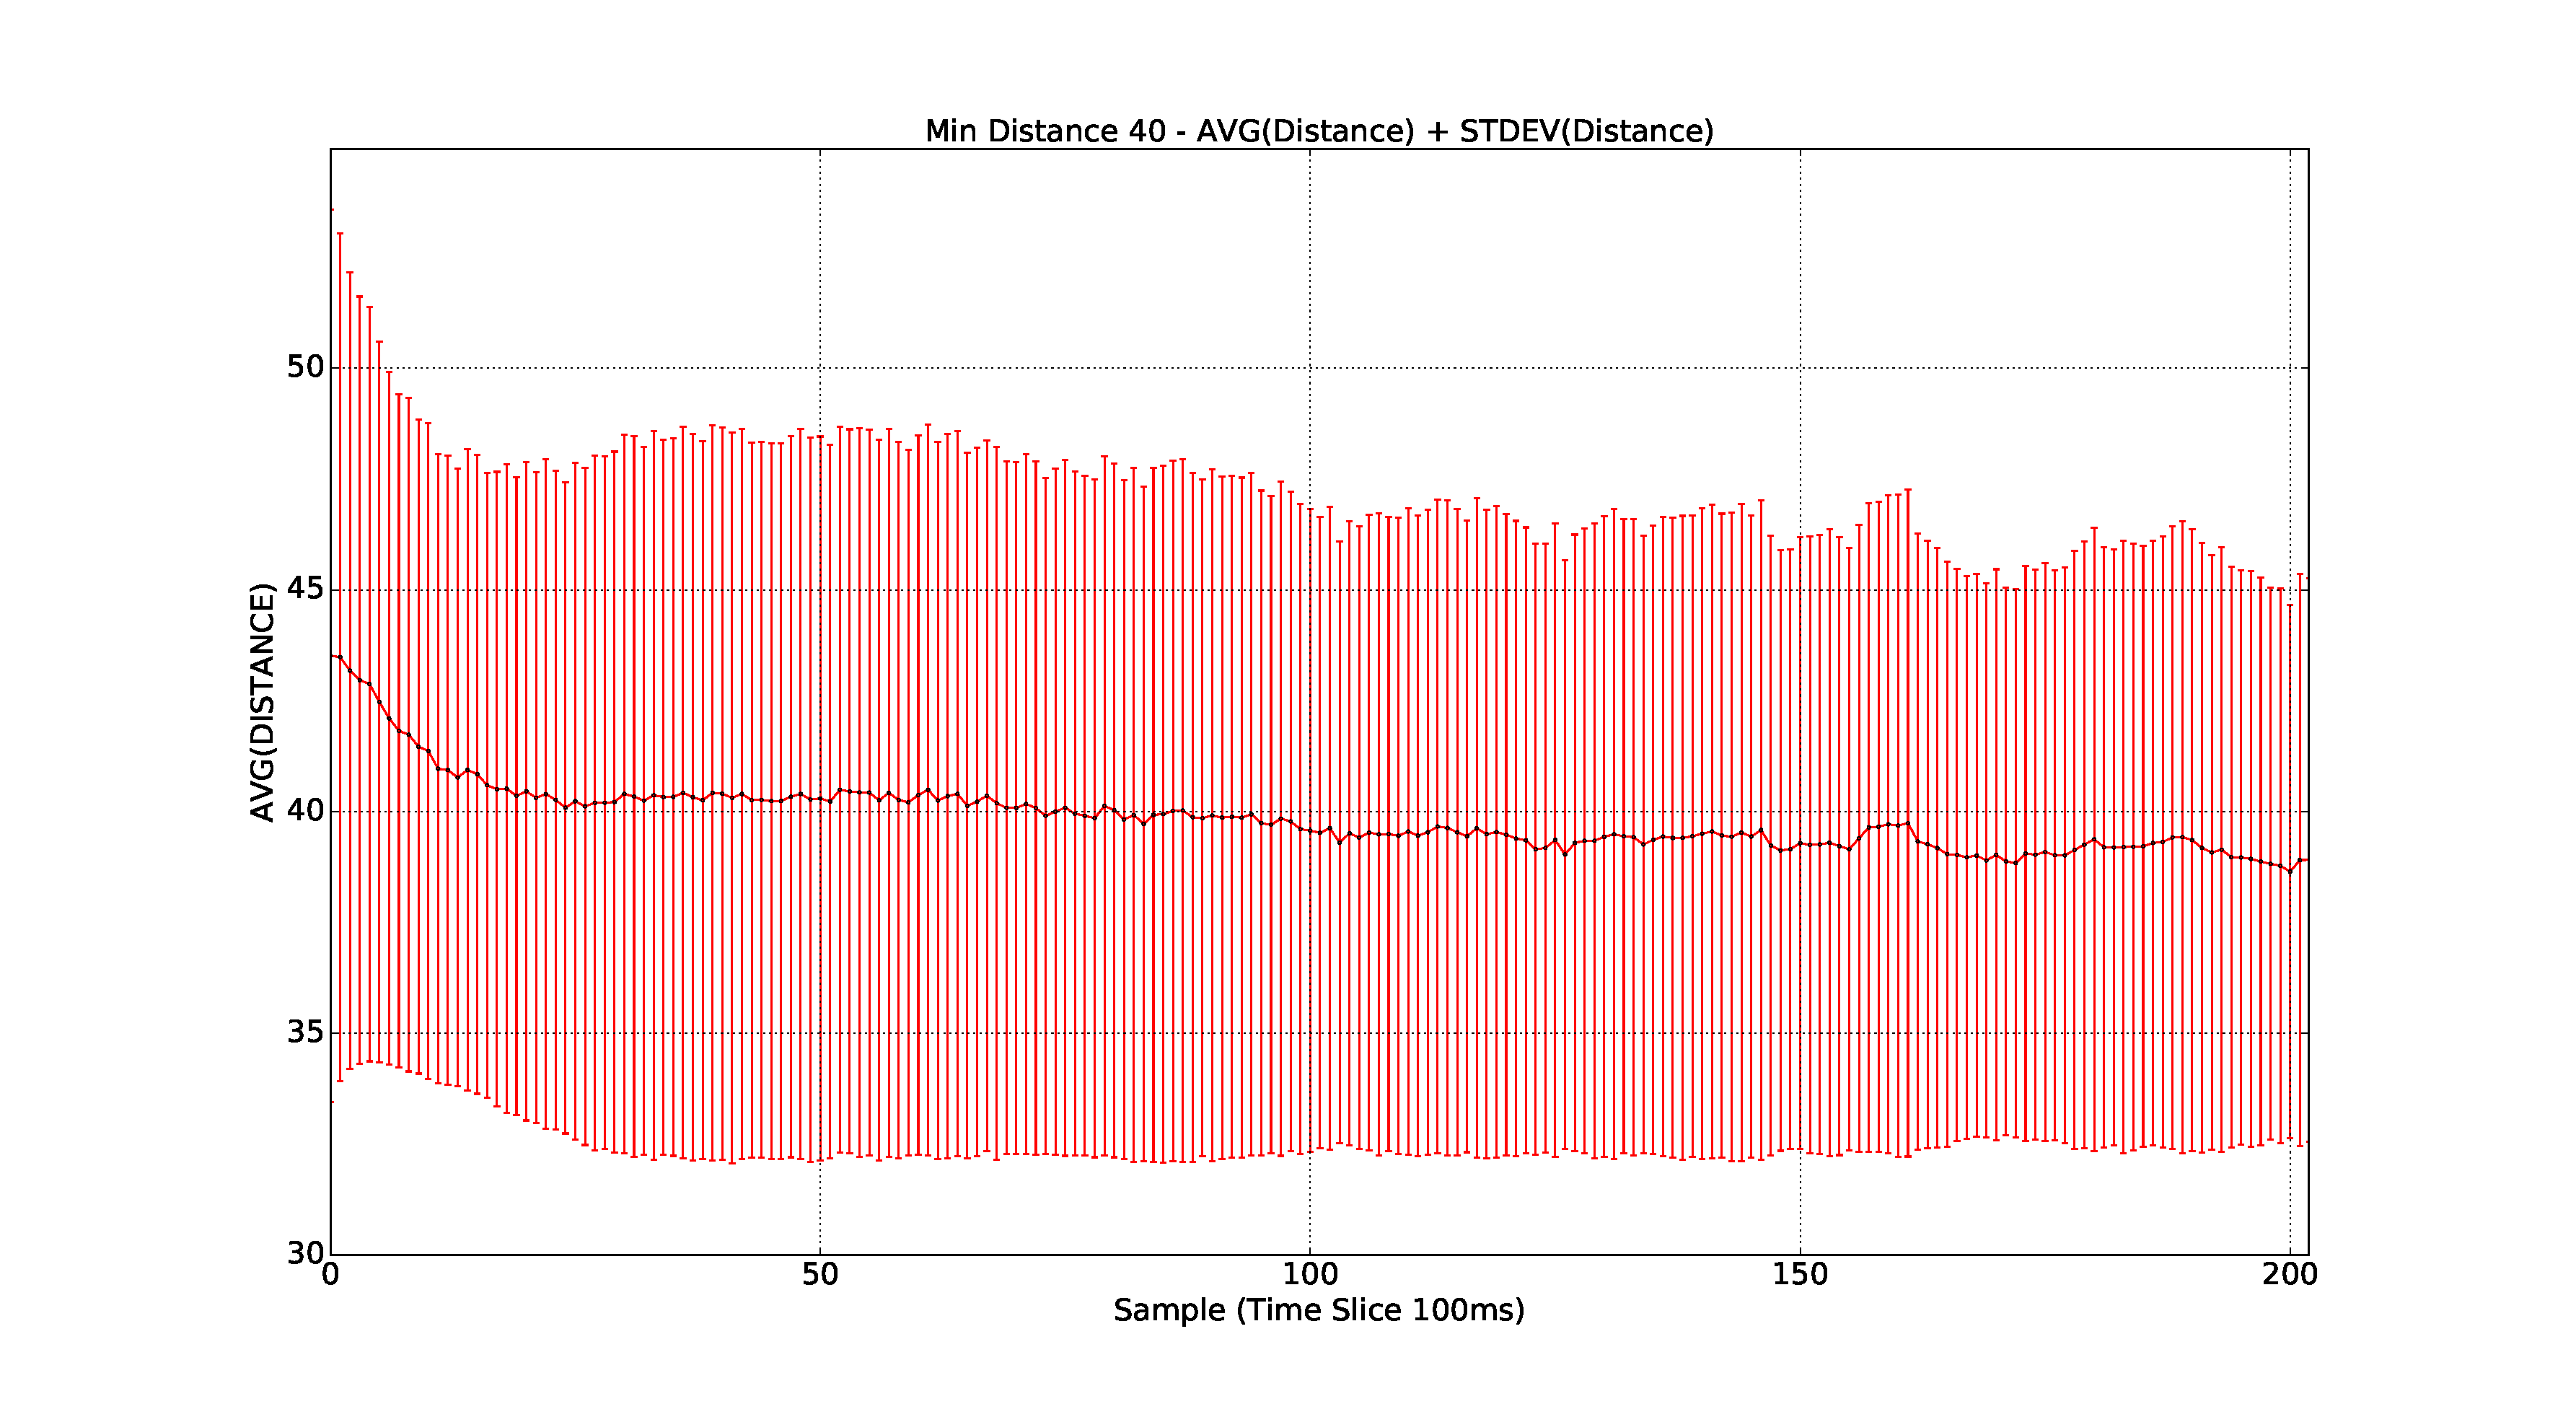
\includegraphics[width=13cm]{CHAPTER-5/figures/StabilityDistanceSwarm40-60}
\end{center}
\caption{Distance metric\label{methods:StabilityDistanceSwarm40-60}}
\end{figure}

\autoref{methods:StabilityDistributionHyper} shows the distribution of the agents over the entire simulation. By looking at the data in terms of the distribution graph it is possible to identify why the standard deviation is greater than that of the hexagonal swarm. The field effects, in this simulation, have created a bi-modal hyper-connected swarm. A bi-modal swarm is created when the agents in a swarm have the cohesion feild effect set such that agents are neighbours one level further out from the immediate neighbours as shown in Figure~\ref{methods:StableSwarmCompressed}. The result of this type of connectivity is that the distribution of the agents distances will produce two peaks in the distribution graph.

%HYPER-DIST-BAR.py
\begin{figure}[H]
\begin{center}
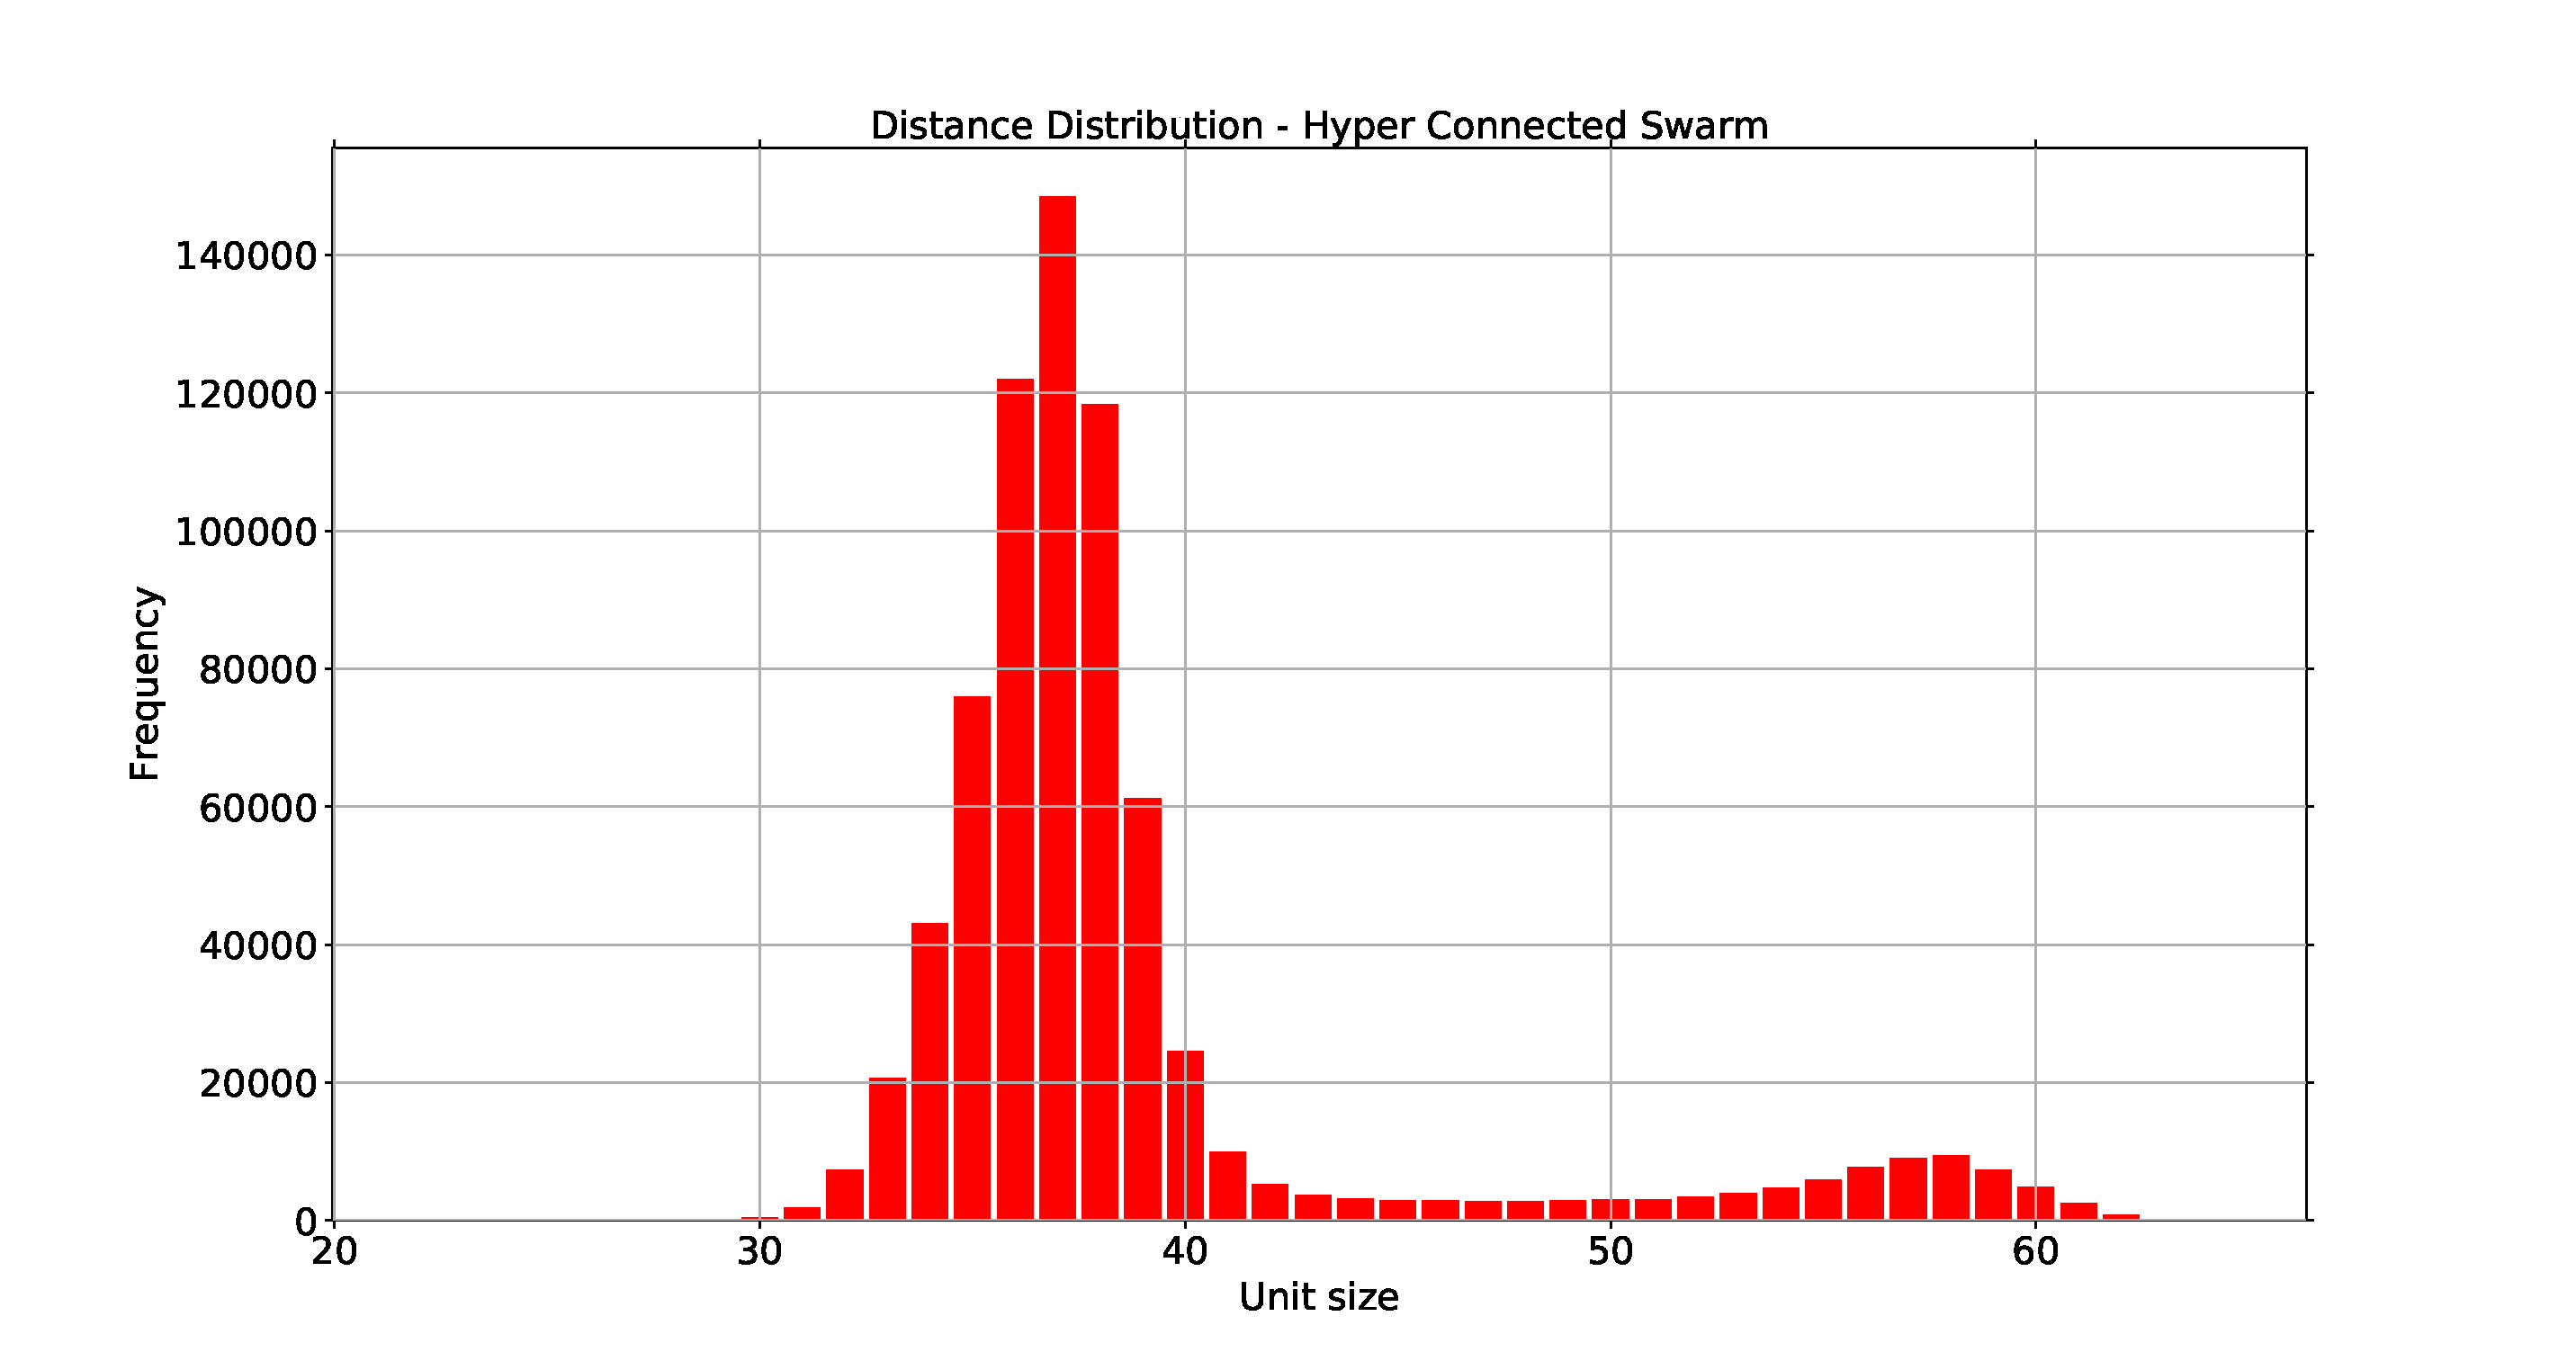
\includegraphics[width=13cm]{CHAPTER-5/figures/StabilityDistibutionHyper}
\end{center}
\caption{Distance distribution\label{methods:StabilityDistributionHyper}}
\end{figure}

\autoref{methods:StabilityDistributionHyper3D} shows the initial distribution of the agents and the progression of the distribution of the swarm agents until 10s into the simulation. The initial state of the distribution at 0s is the same for both swarm types. The impact of the field effects are immediate as the swarm stabilises to a bi-modal distribution. \autoref{methods:StabilityDistributionHyper3D2} shows the distribution of the data at 10 seconds (100 cycles) showing the resultant bi-modal frequencies the swarm is therefore a hyper-connected swarm.
%HYPER-DIST-BAR-3D.py
\begin{figure}[H]
\begin{center}
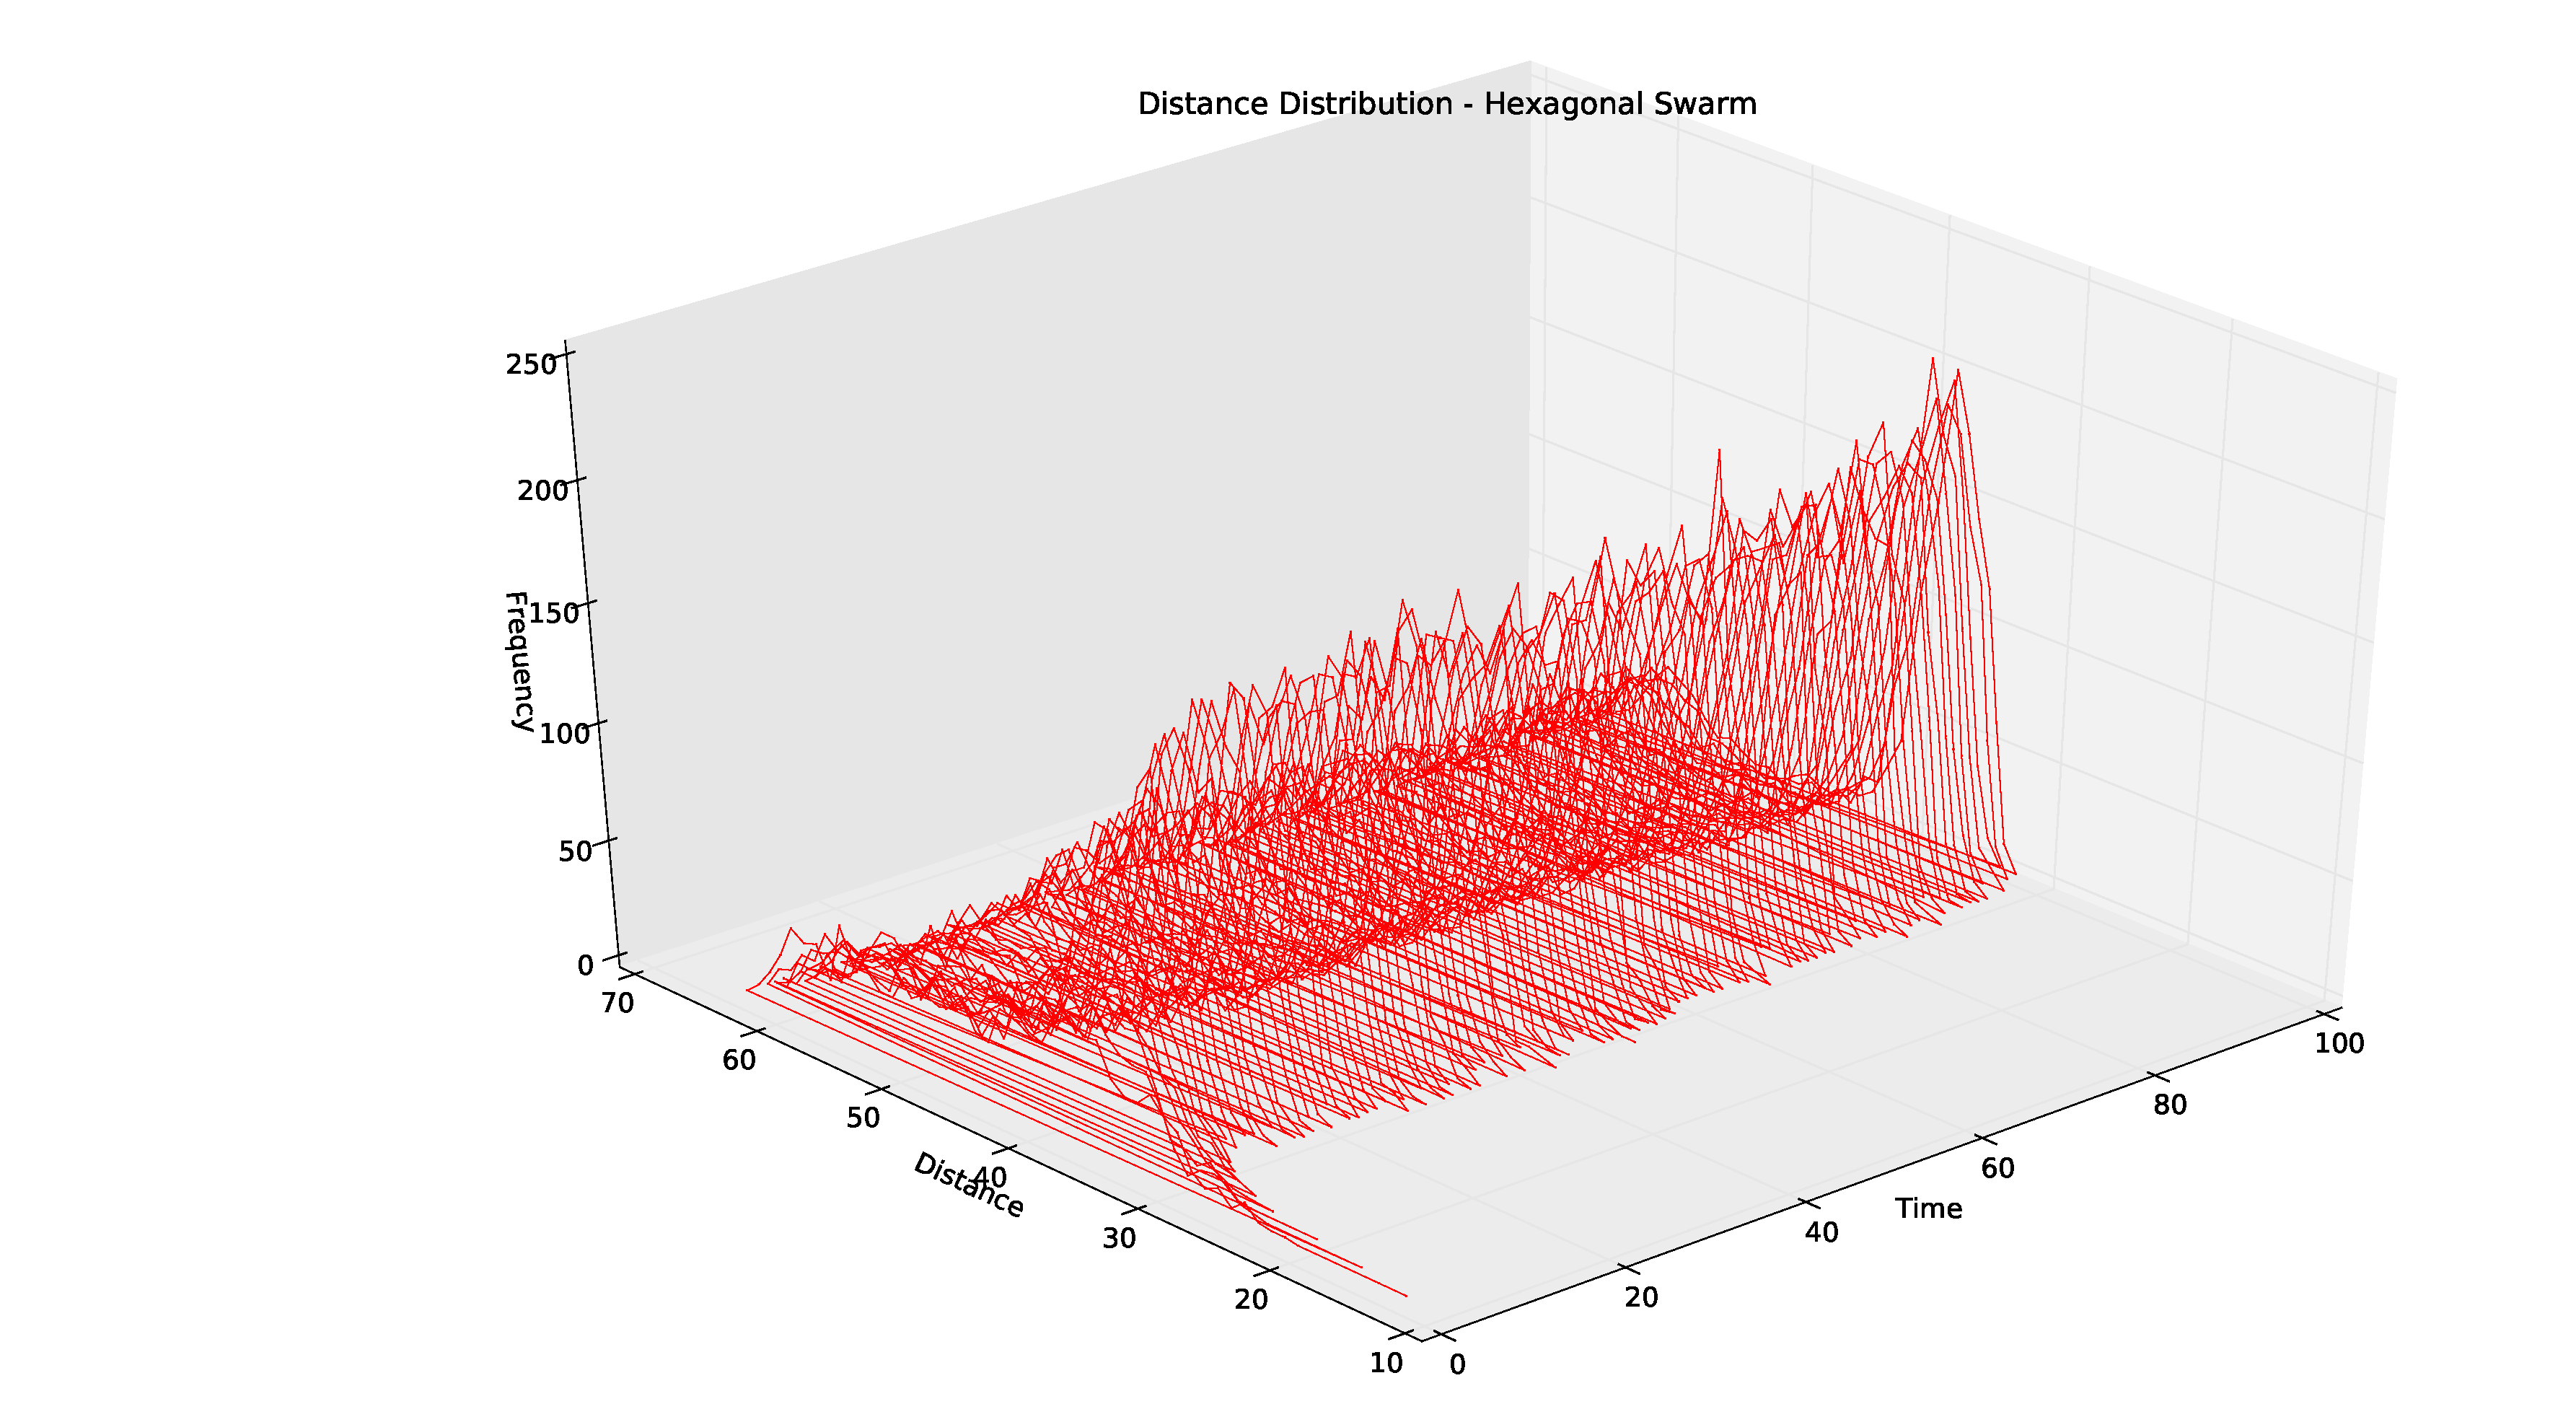
\includegraphics[width=13cm]{CHAPTER-5/figures/StabilityDistibutionHyper3D}
\end{center}
\caption{Distance distribution / Time 0-10 seconds\label{methods:StabilityDistributionHyper3D}}
\end{figure}

\begin{figure}[H]
\begin{center}
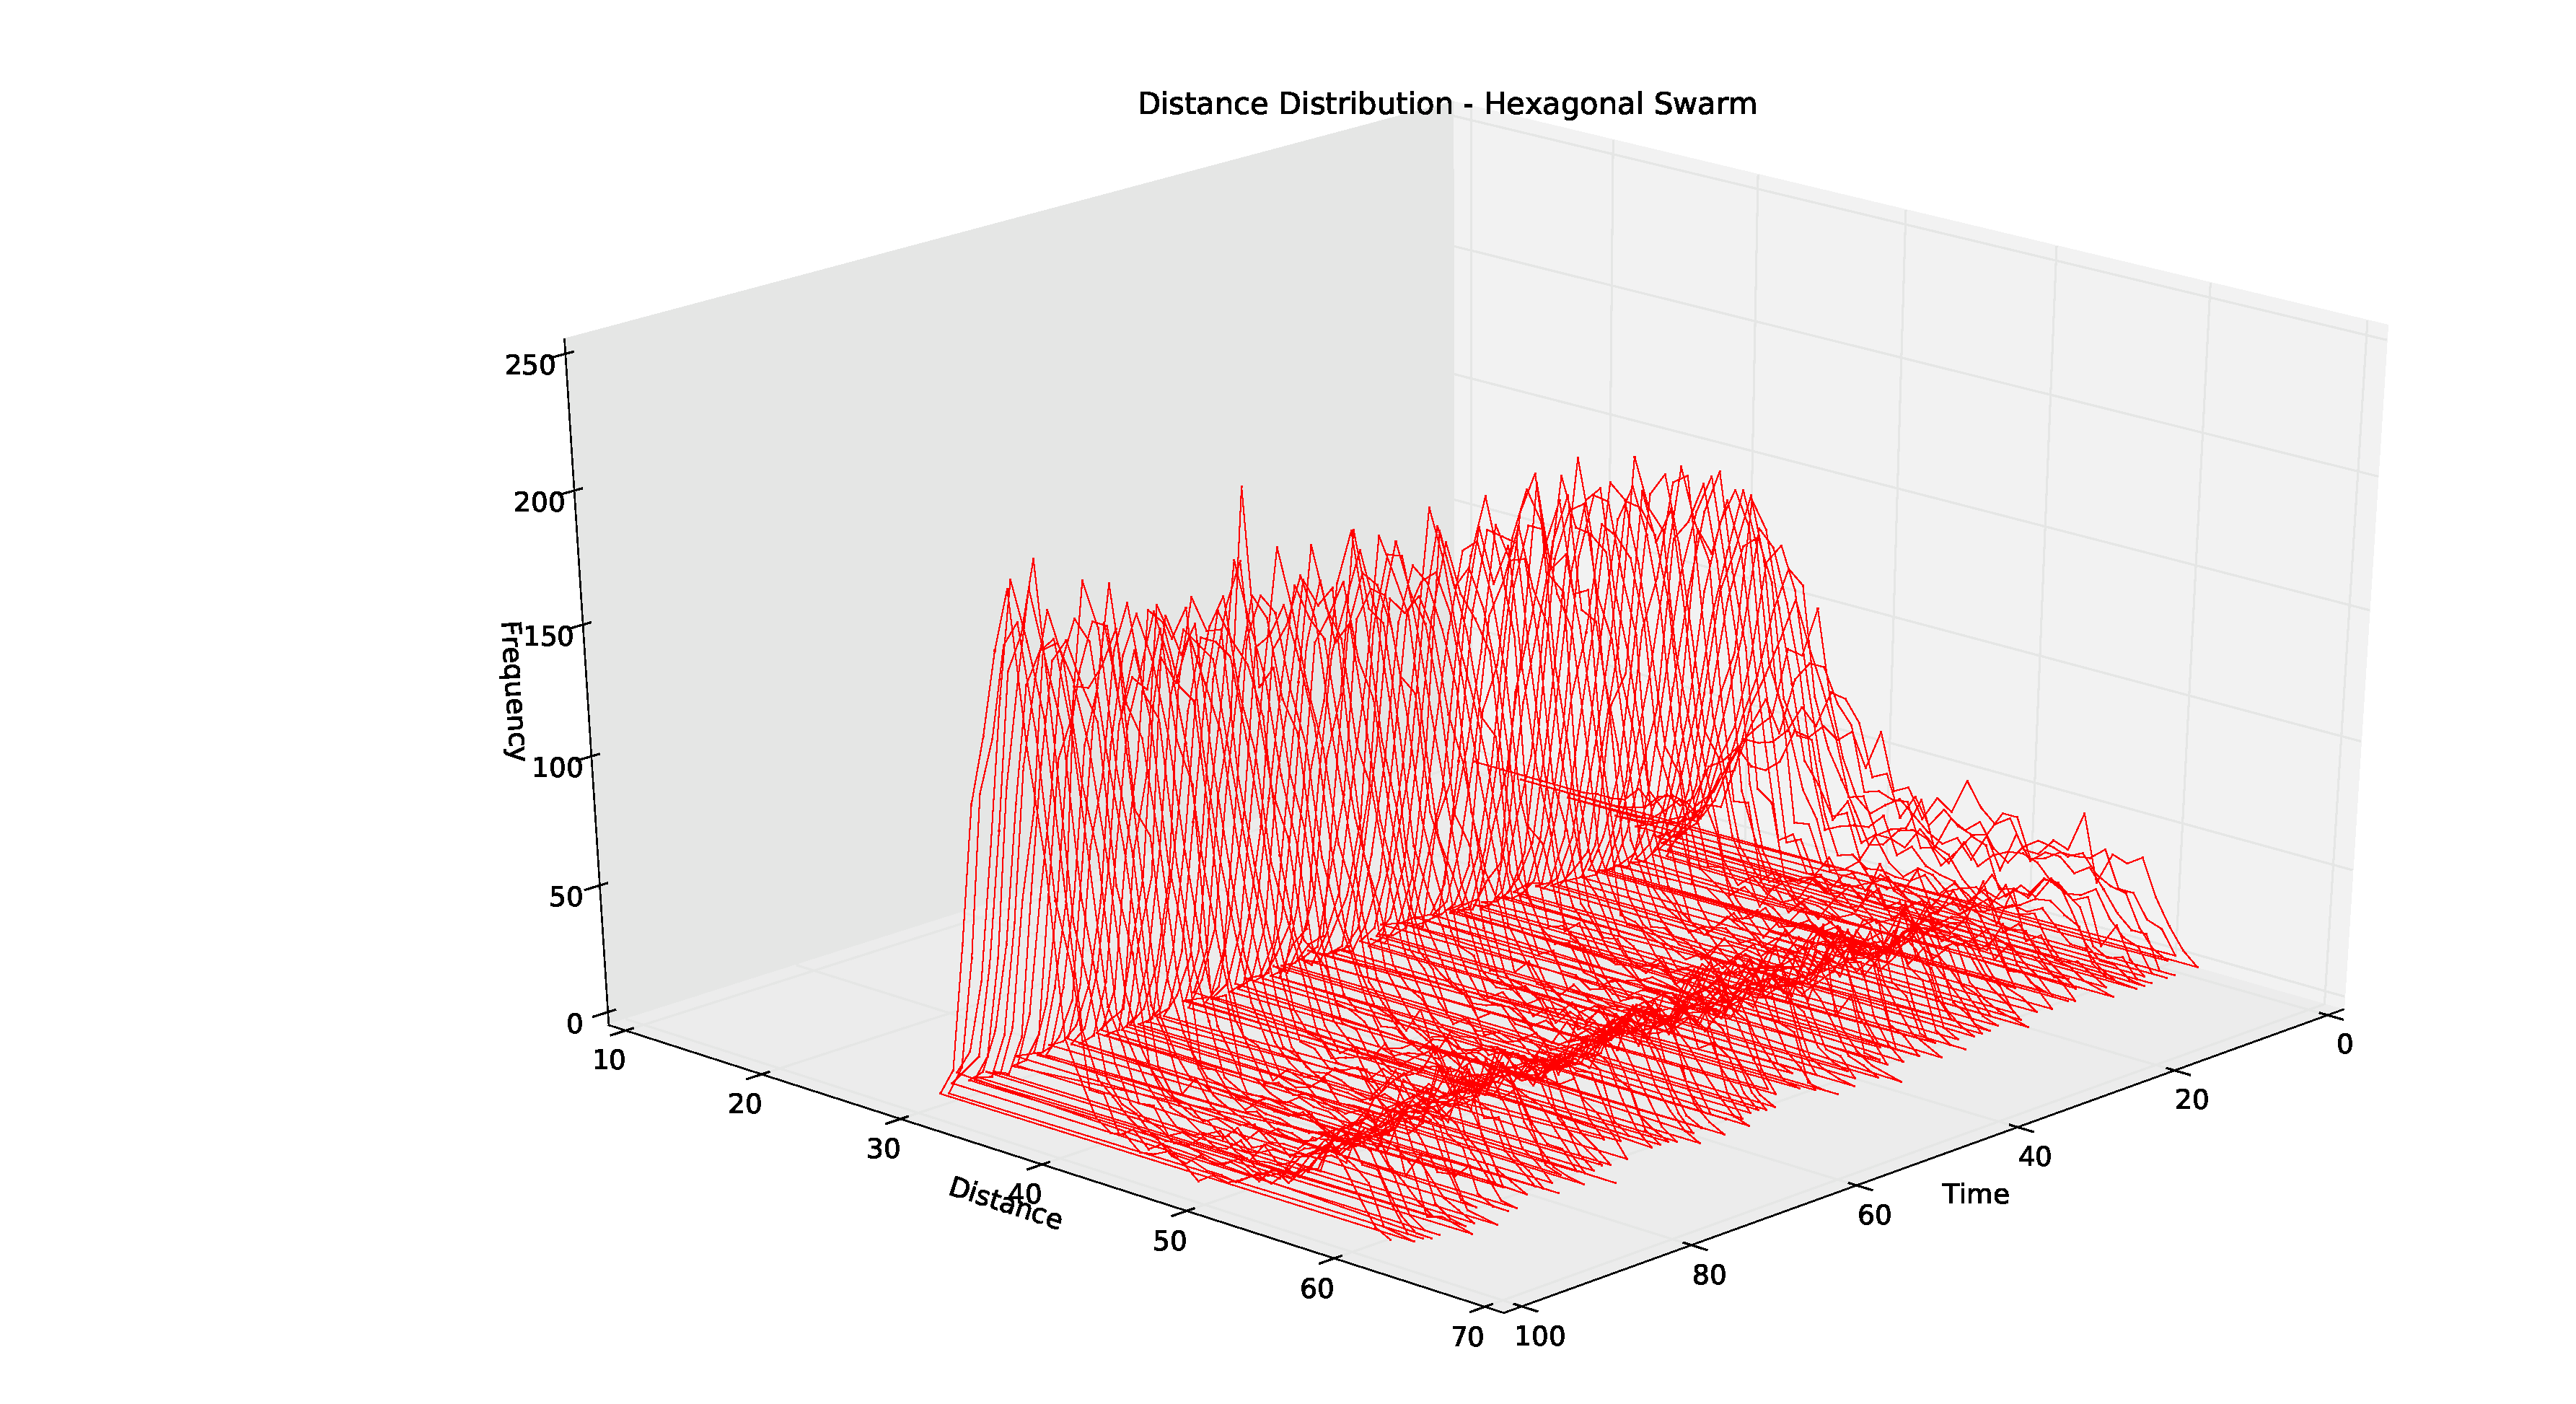
\includegraphics[width=13cm]{CHAPTER-5/figures/StabilityDistibutionHyper3D2}
\end{center}
\caption{Distance distribution / Time 10-0 seconds\label{methods:StabilityDistributionHyper3D2}}
\end{figure}

Although the field effects in this simulation have produced a bi-modal distribution increasing the neighbour distance will create further swarm types that will be multi-modal as more distant agents are identified as neighbours.

\subsection{Agent resultant magnitude based metric}
The distribution of the potential magnitudes can be visualised in the same way as the distances. \autoref{methods:StabilityMagnitudeHyper} shows the distribution of the agents based on potential magnitude for the entire duration of the simulation. As with the distance based metric the data forms a bi-modal distribution with a mean magnitude as shown in \autoref{methods:StabilityMagnitude40-60}. \autoref{methods:StabilityMagnitudeHyper} shows negative magnitudes which indicates sections of the swarm are expanding. 
%HYPER-MAG.py
\begin{figure}[H]
\begin{center}
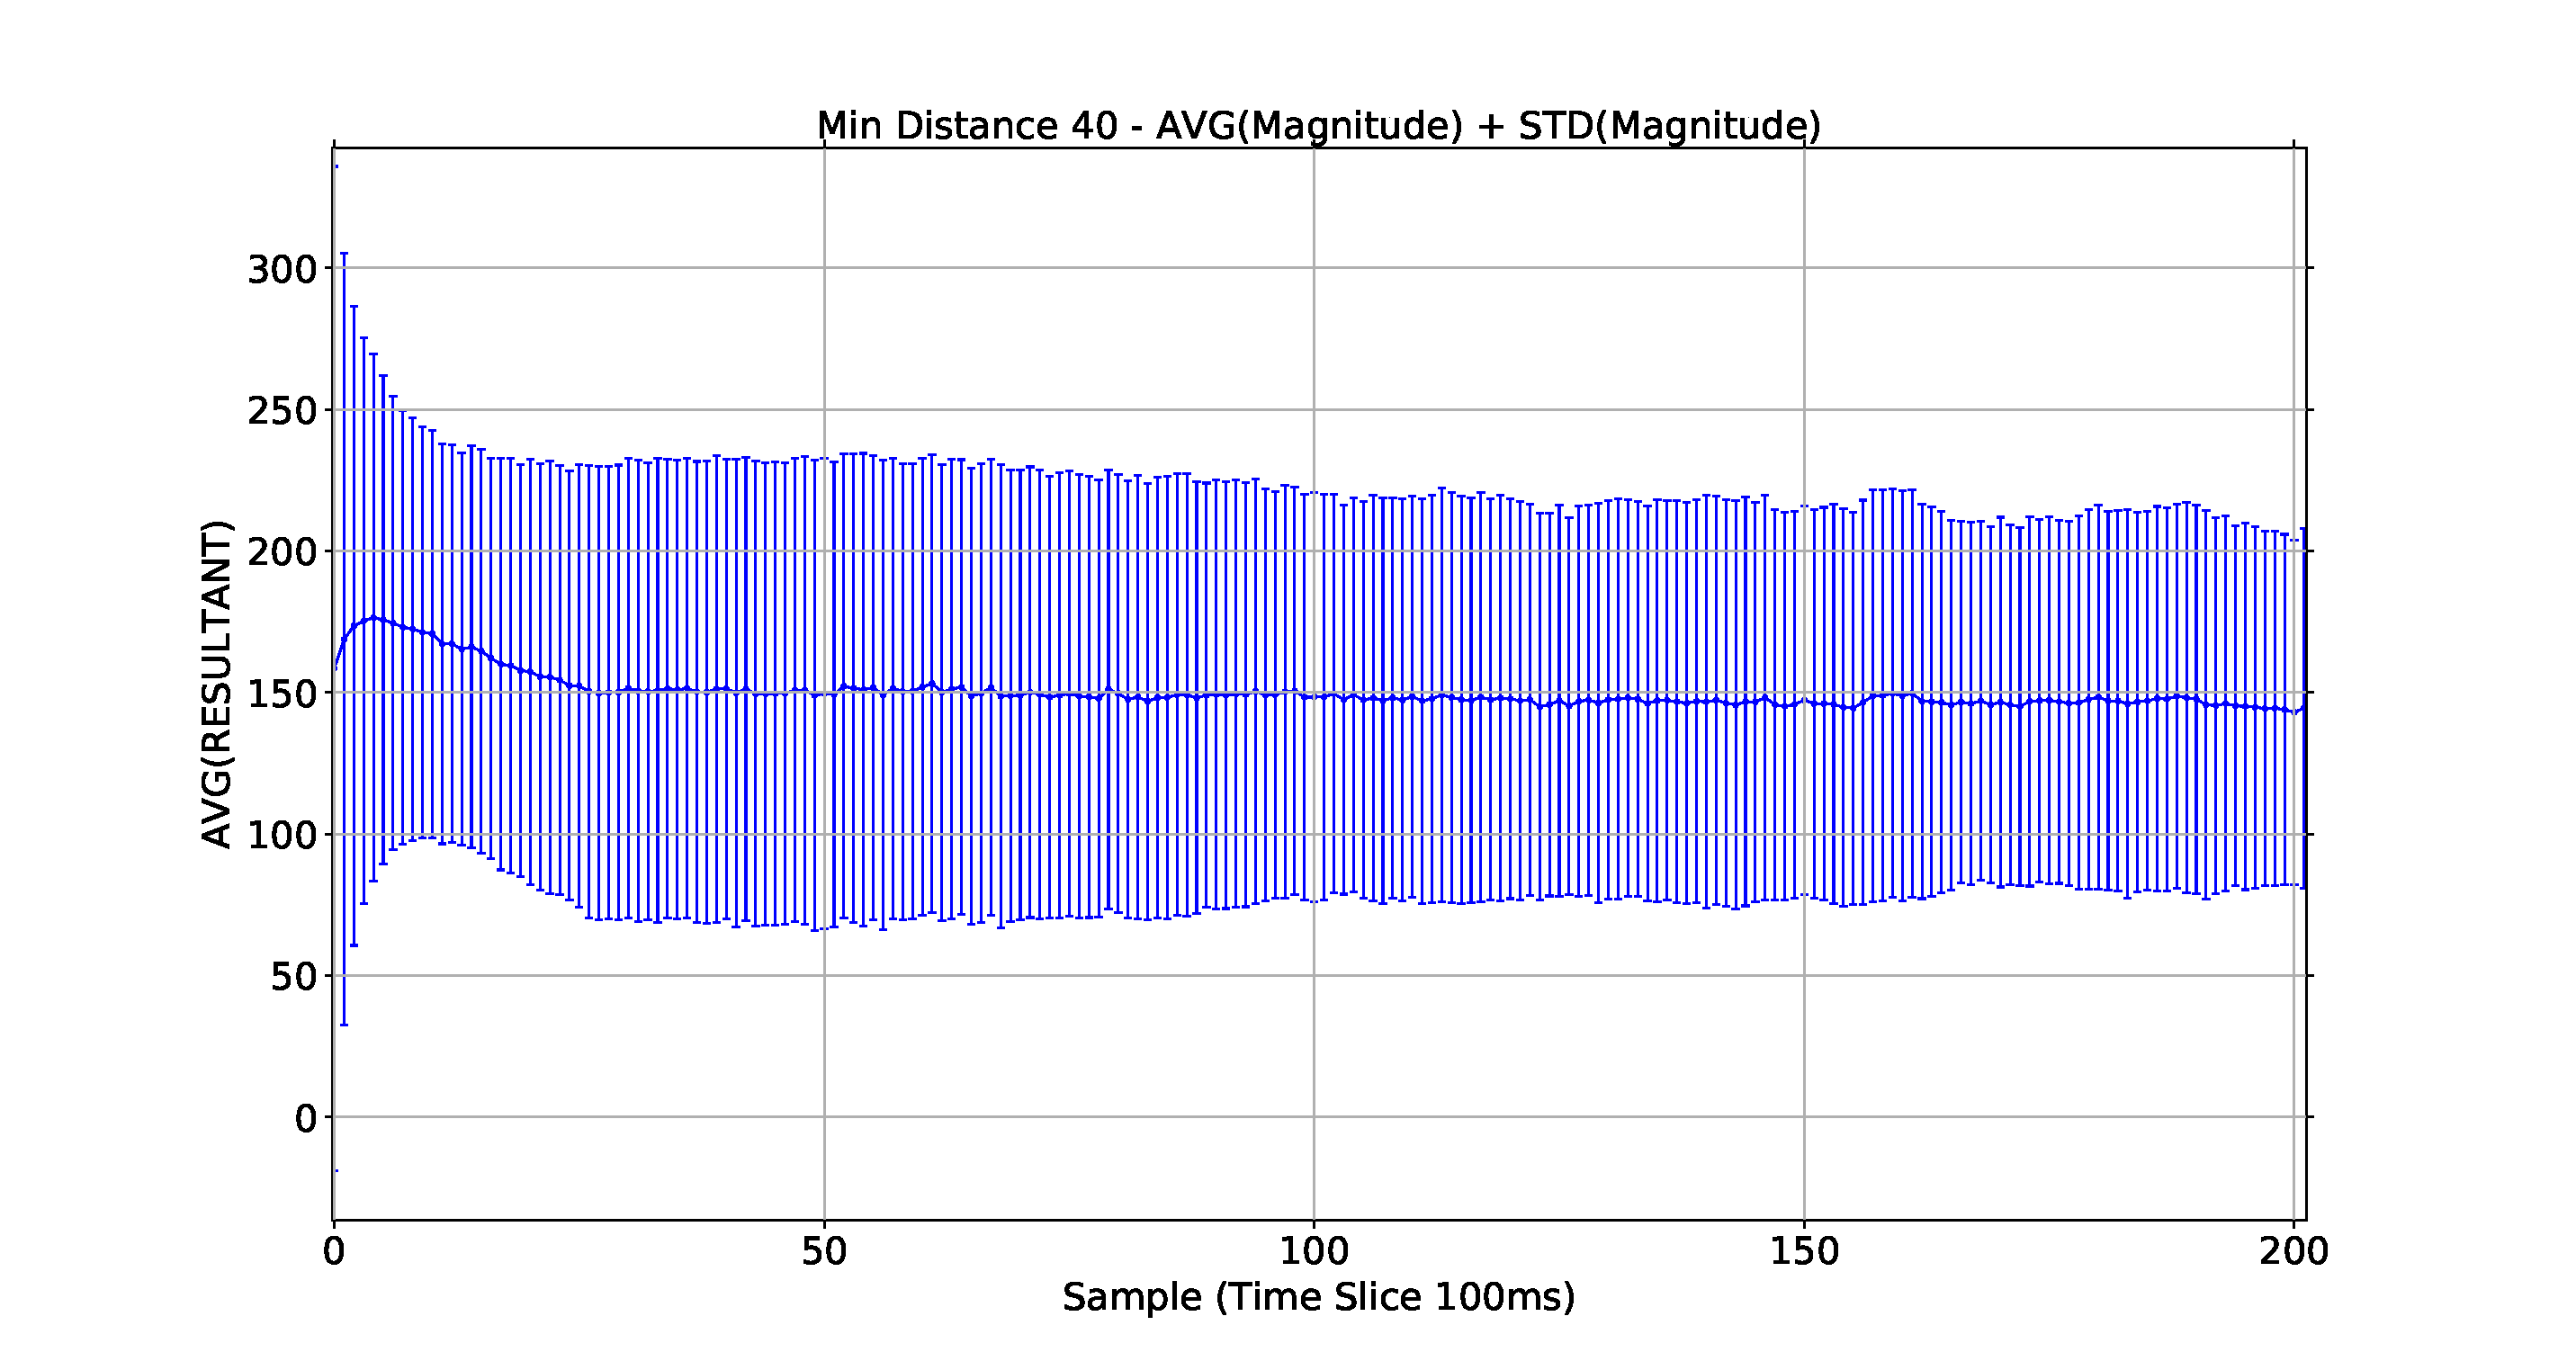
\includegraphics[width=13cm]{CHAPTER-5/figures/StabilityMagnitudeSwarm40-60}
\end{center}
\caption{Agent resultant magnitude metric\label{methods:StabilityMagnitude40-60}}
\end{figure}
%HYPER-MAG-BAR.py 
\begin{figure}[H]
\begin{center}
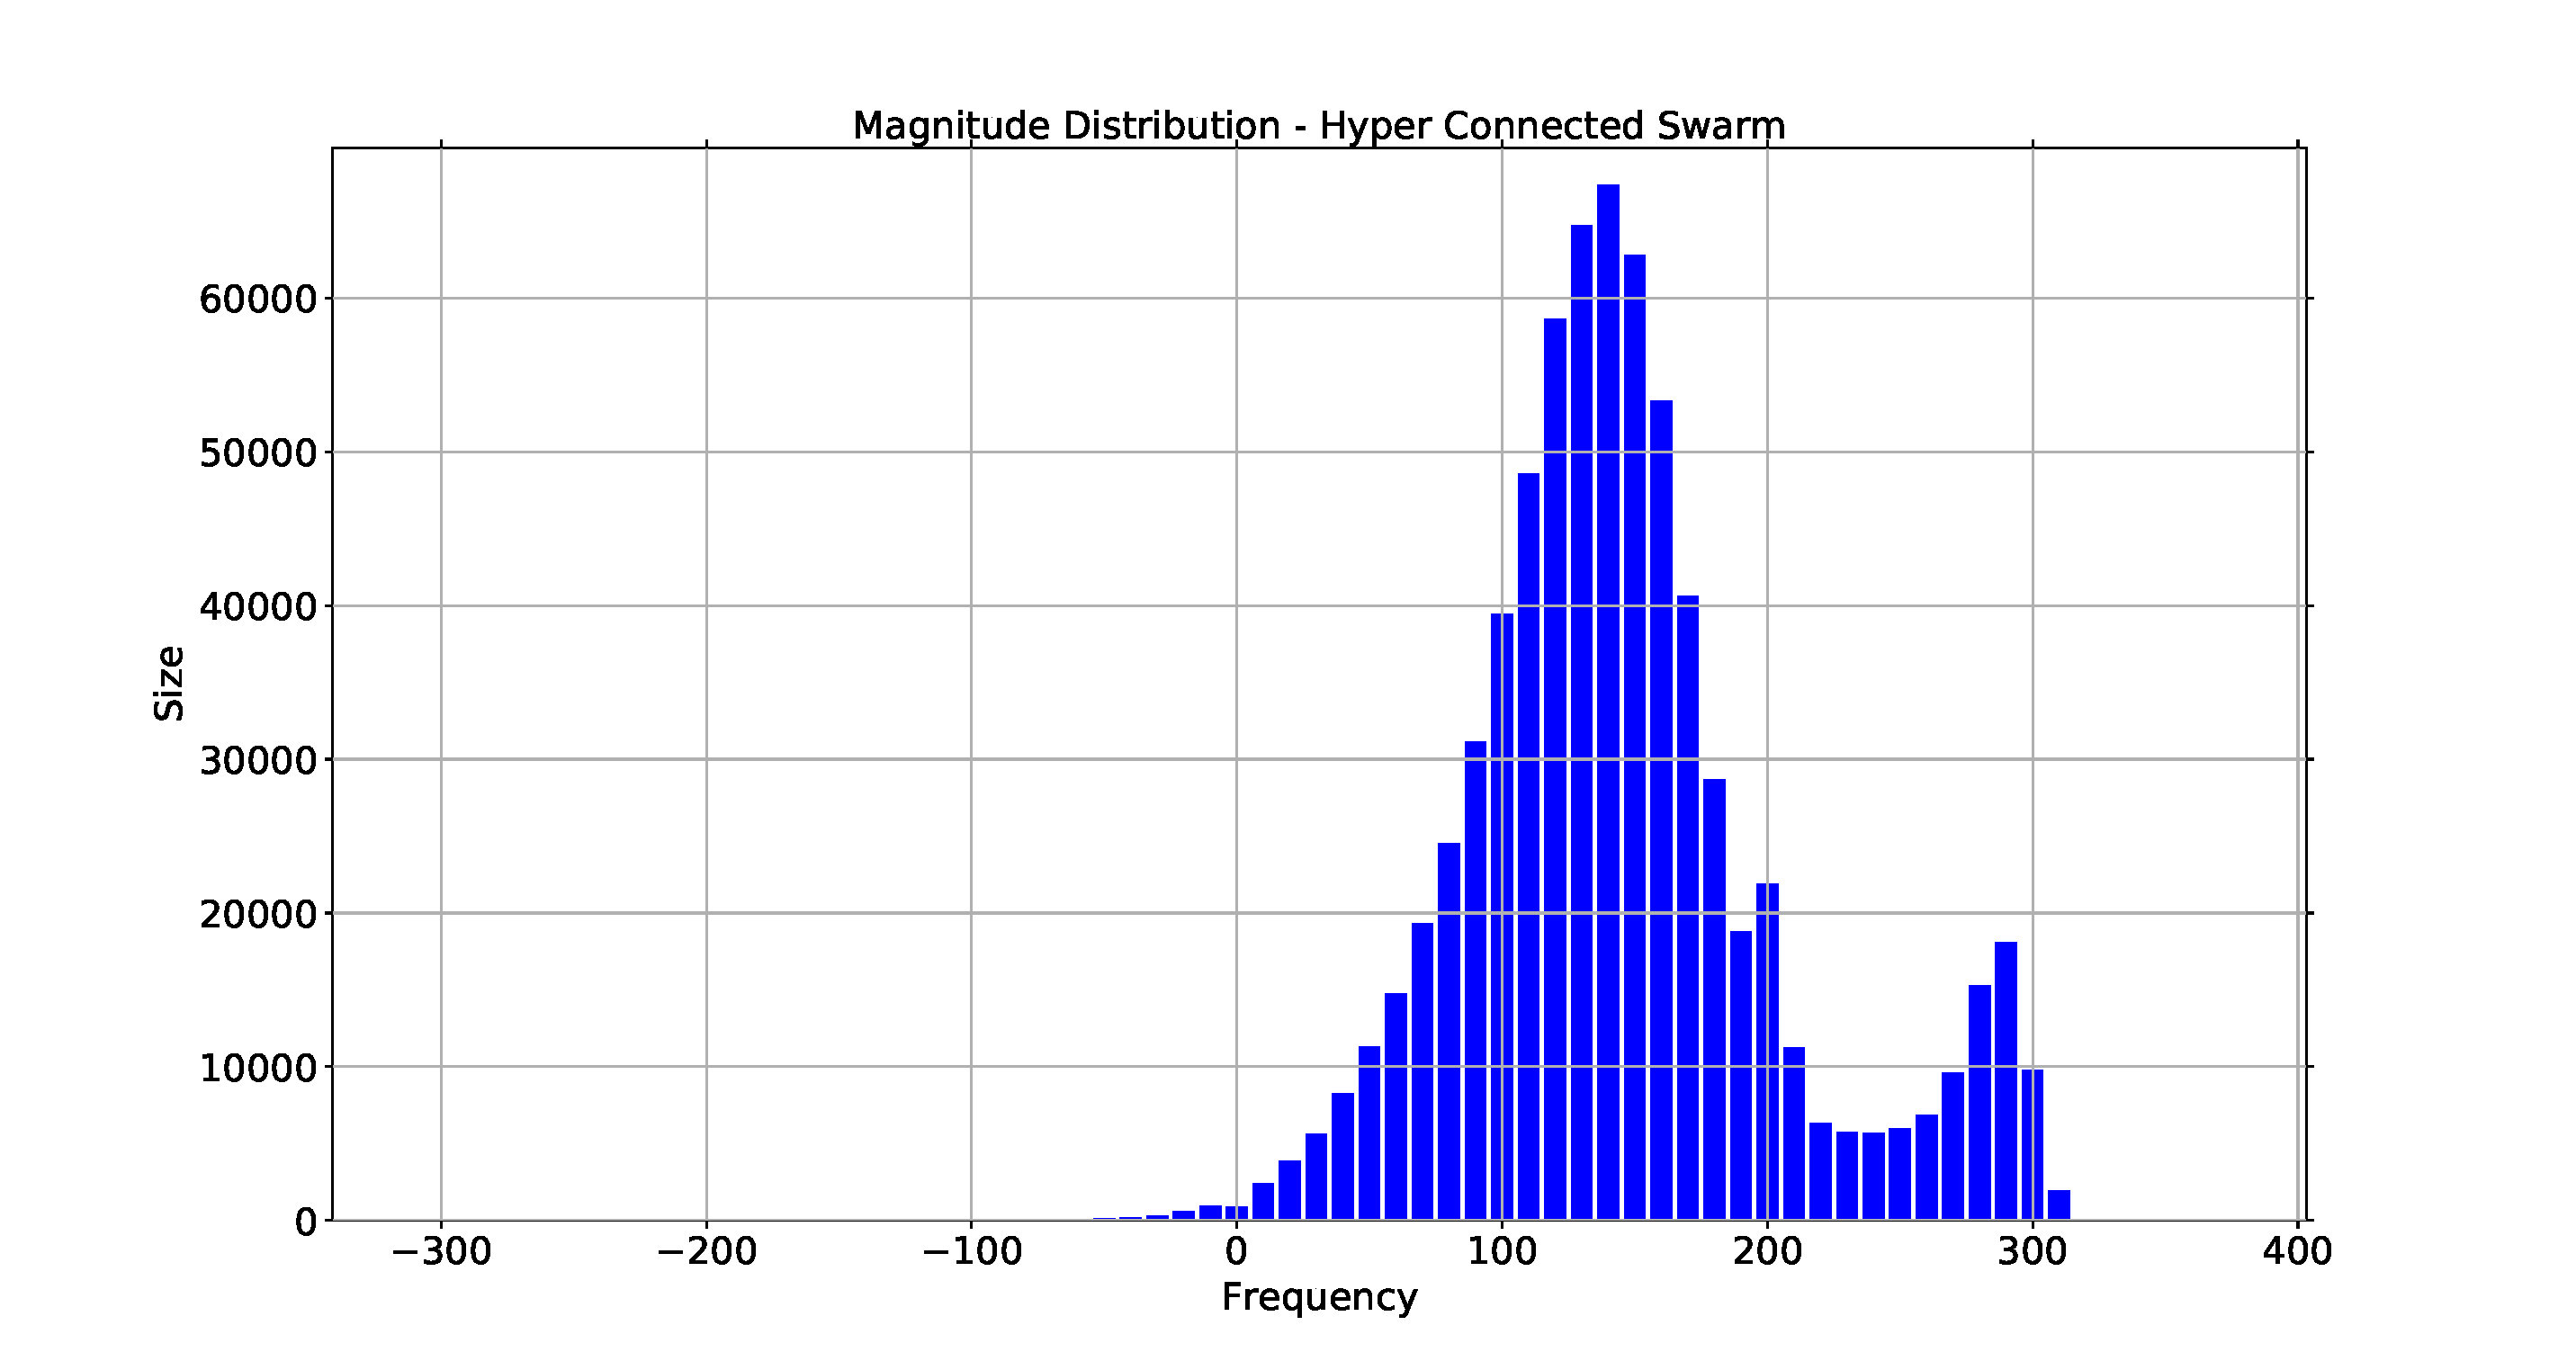
\includegraphics[width=13cm]{CHAPTER-5/figures/StabilityMagnitudeHyper}
\end{center}
\caption{Agent resultant magnitude distribution\label{methods:StabilityMagnitudeHyper}}
\end{figure}

\autoref{methods:StabilityMagHyper3D} and \ref{methods:StabilityMagHyper3D2} show the distributions at each time cycle and visualise the change in the distributions of the agent resultant magnitudes. As with the distance visualisations \autoref{methods:StabilityMagHyper3D} shows the initial distribution at time interval 0 to 100 and \autoref{methods:StabilityMagHyper3D2} shows the final state of the swarm after 10 seconds (100 cycles). Both show the bi-model state of the swarm emerging.
%HYPER-MAG-BAR-3D.py
\begin{figure}[H]
\begin{center}
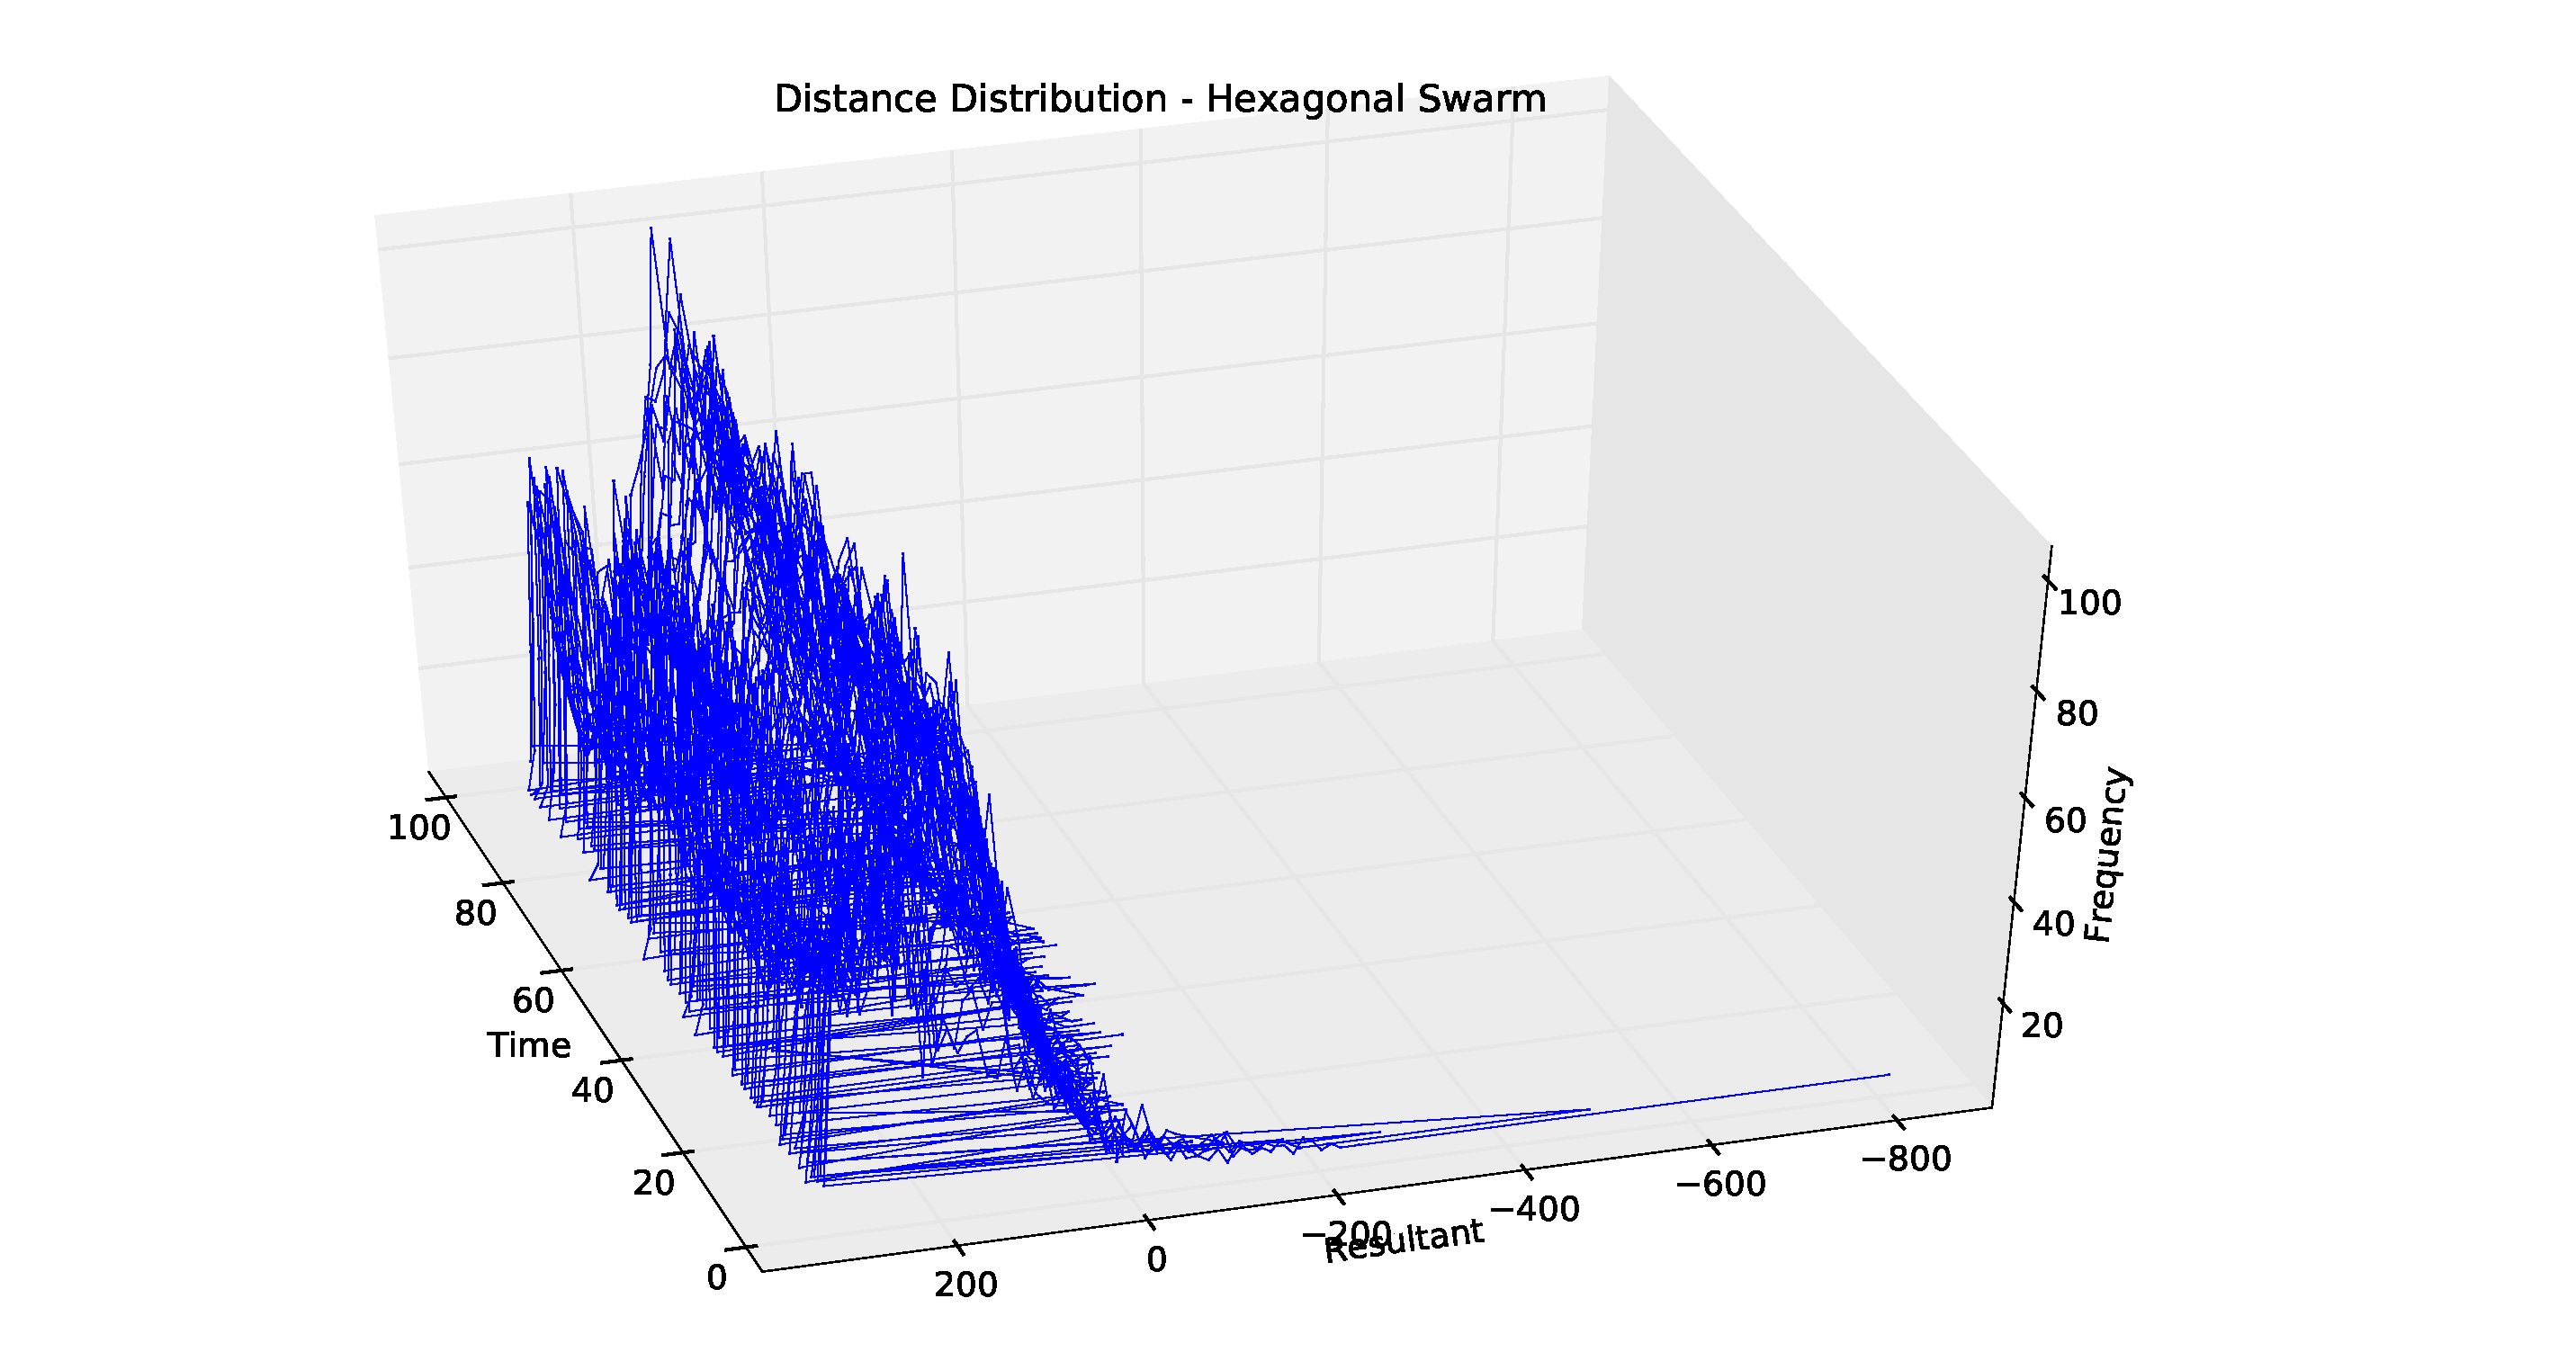
\includegraphics[width=13cm]{CHAPTER-5/figures/StabilityMagHyper3D}
\end{center}
\caption{Agent resultant magnitude distribution / Time 0-10s\label{methods:StabilityMagHyper3D}}
\end{figure}

\begin{figure}[H]
\begin{center}
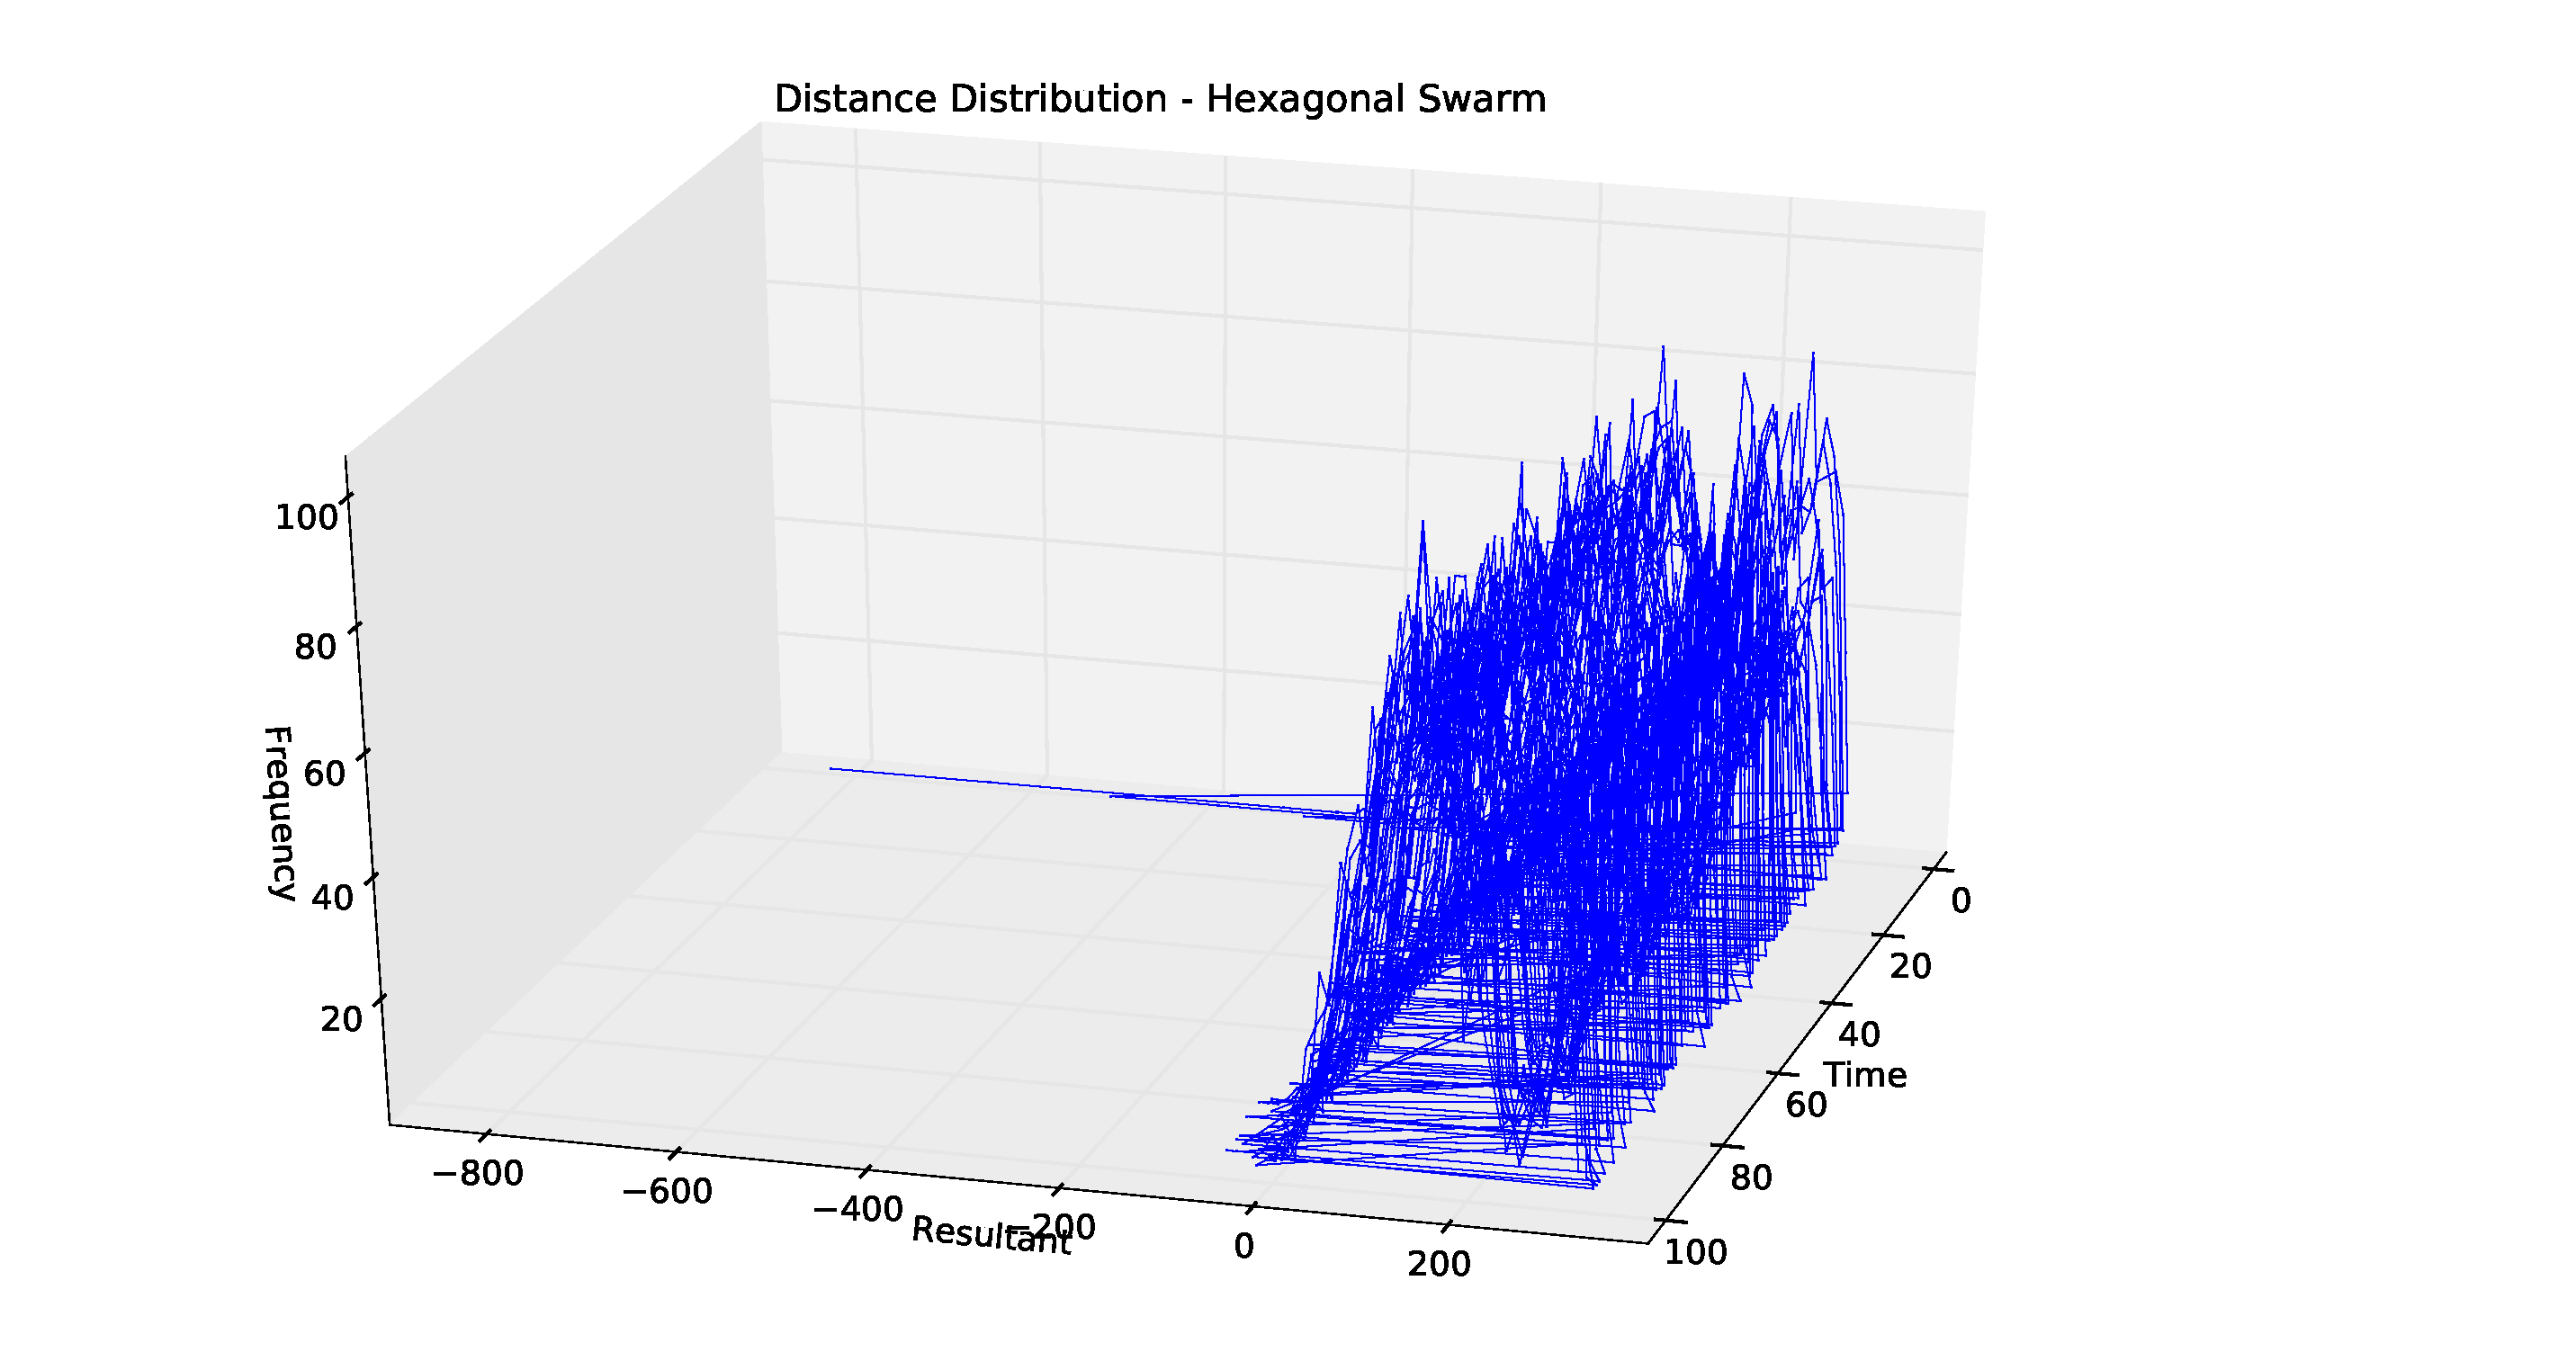
\includegraphics[width=13cm]{CHAPTER-5/figures/StabilityMagHyper3D2}
\end{center}
\caption{Agent resultant magnitude distribution / Time 10-0s\label{methods:StabilityMagHyper3D2}}
\end{figure}

\section{Metric comparison\label{section:stabilityComparison}}
Looking at the two swarm types together the characteristics of the swarm types present themselves as change in the standard deviation from either the average distance or the average magnitude of the agents in the swarm.

\autoref{methods:StabilityDistanceSwarm40-5060} shows the swarm with the two different field effects for cohesion. The metric used in this analysis is the distance between agents. The result shows that the deviation on the hyper-connected swarm (shown in green) has a higher standard deviation than the hexagonal swarm (shown in brown). This is caused by the bi-modal nature of the hyper-connected swarm.

\autoref{methods:StabilityMagnitudeSwarm40-5060} shows the analysis of the agent resultant magnitude between the agents in the swarm which demonstrates the same characteristic emerging.
%HEX-HYPER.py
\begin{figure}[H]
\begin{center}
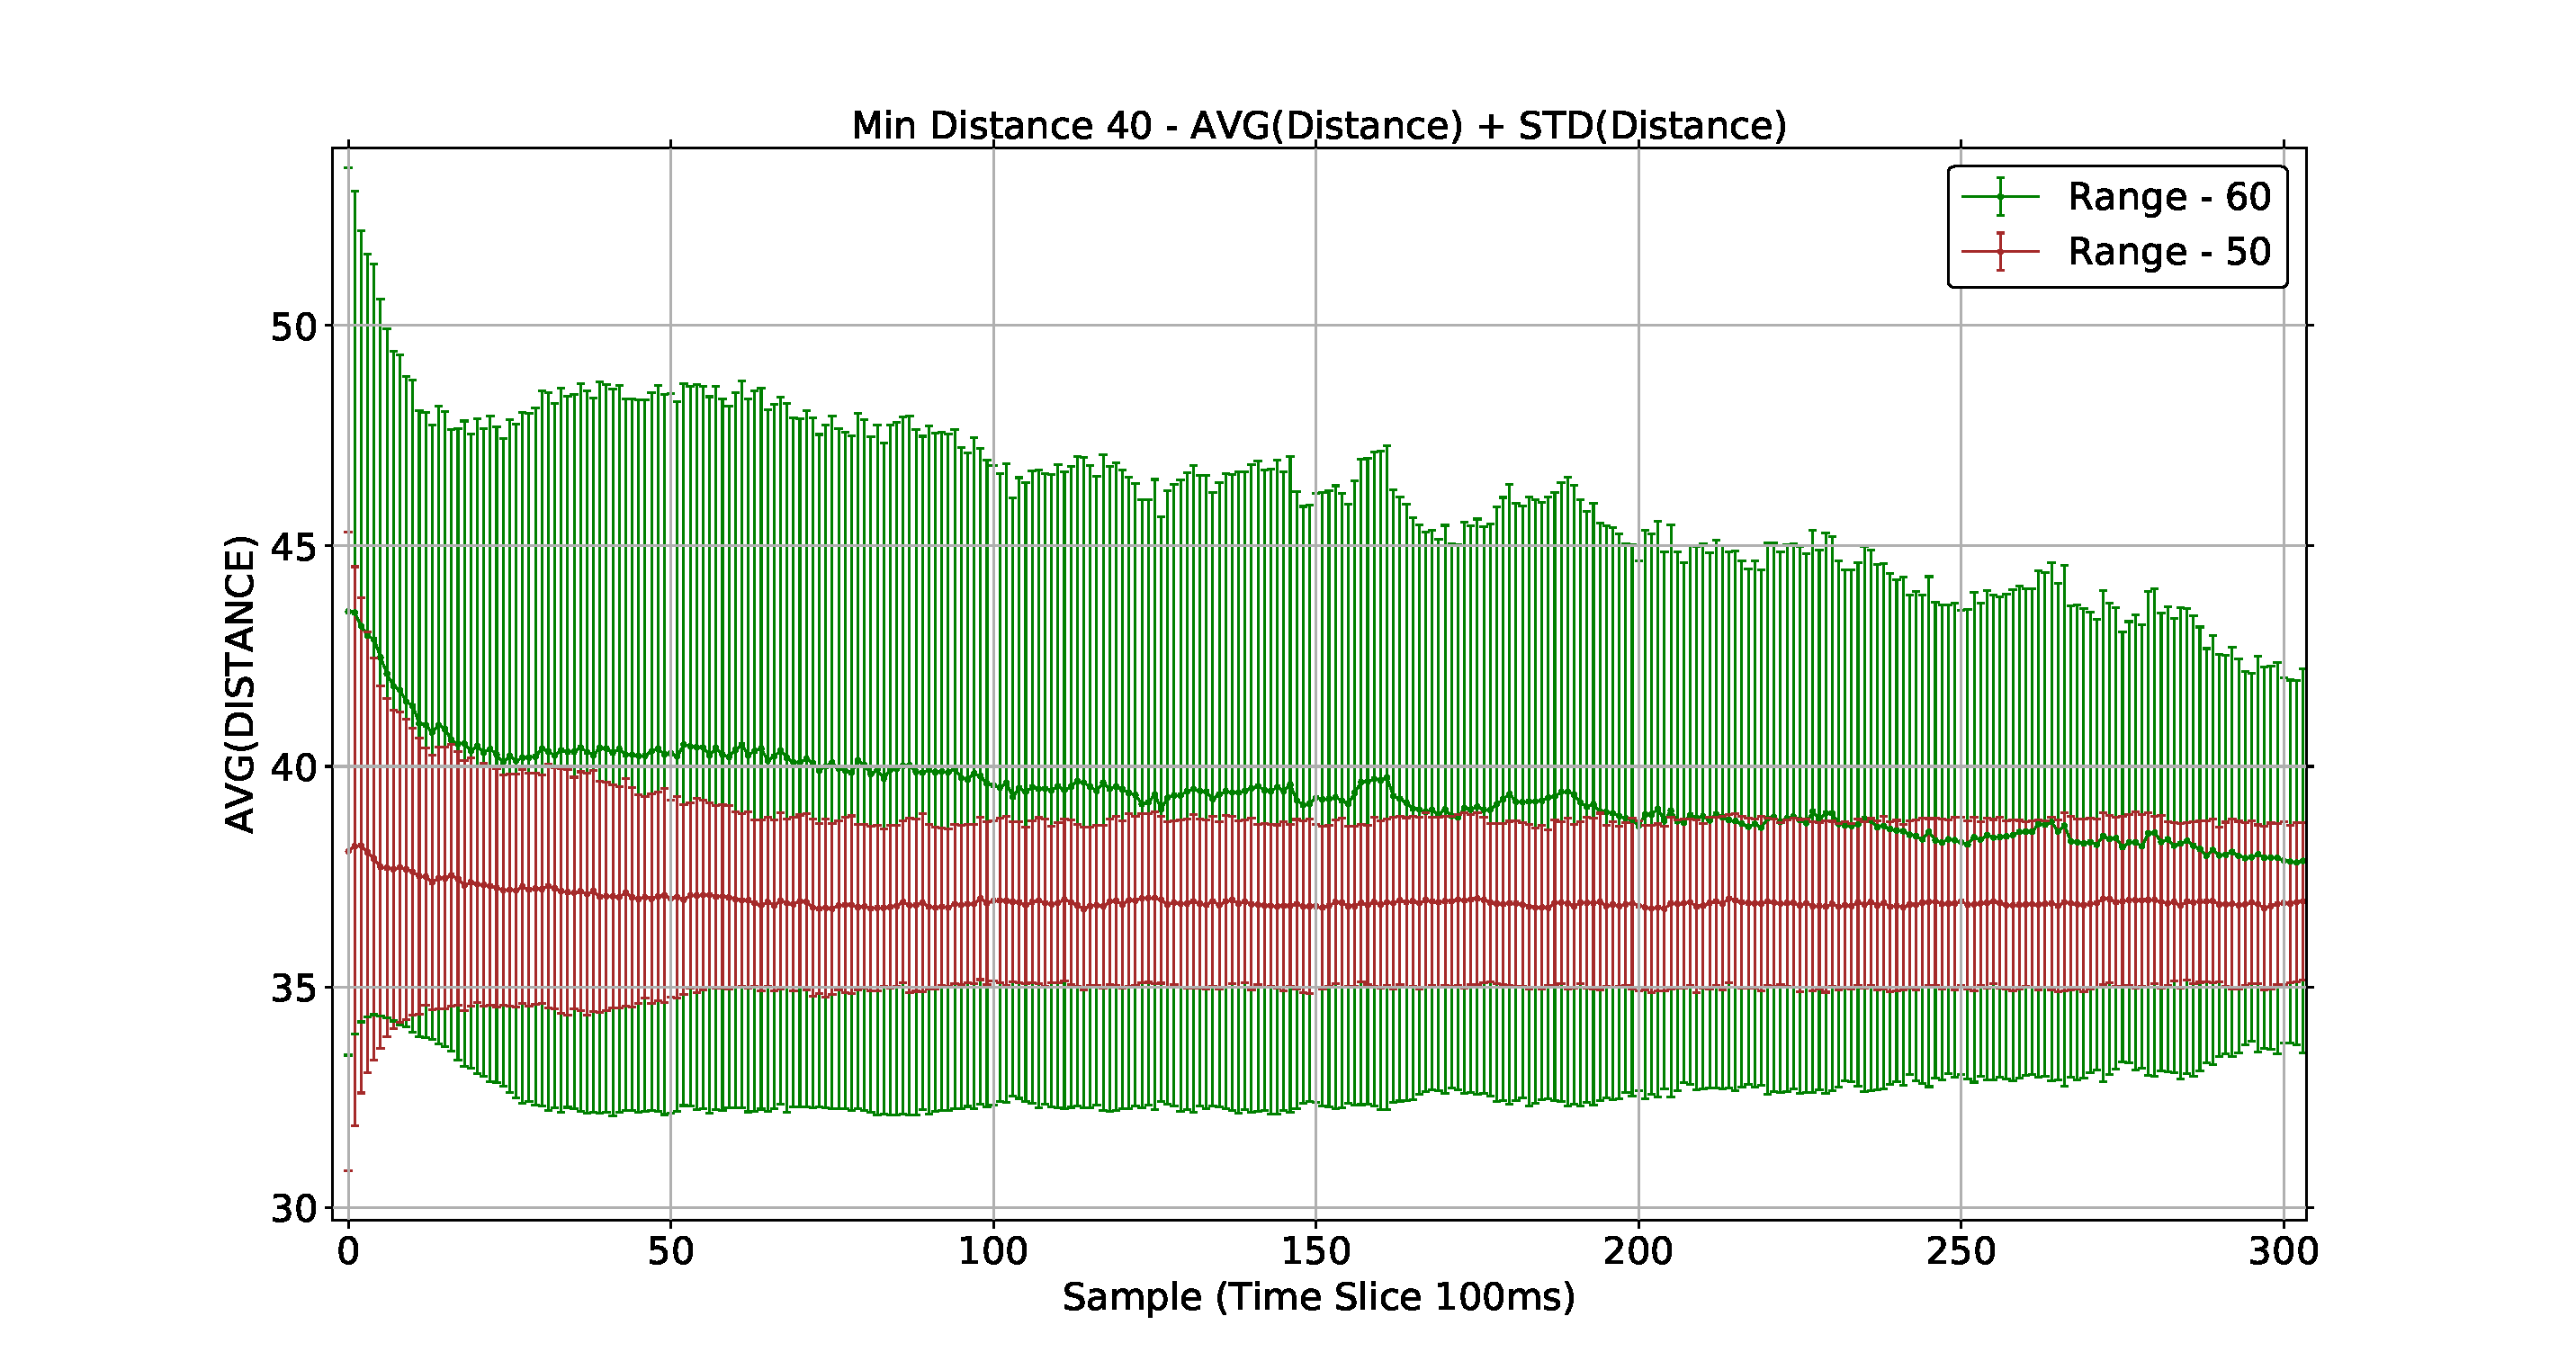
\includegraphics[width=13cm]{CHAPTER-5/figures/StabilityDistanceSwarm40-5060}
\end{center}
\caption{Distances metric comparison\label{methods:StabilityDistanceSwarm40-5060}}
\end{figure}
%HEX-HYPER-MAG.py
\begin{figure}[H]
\begin{center}
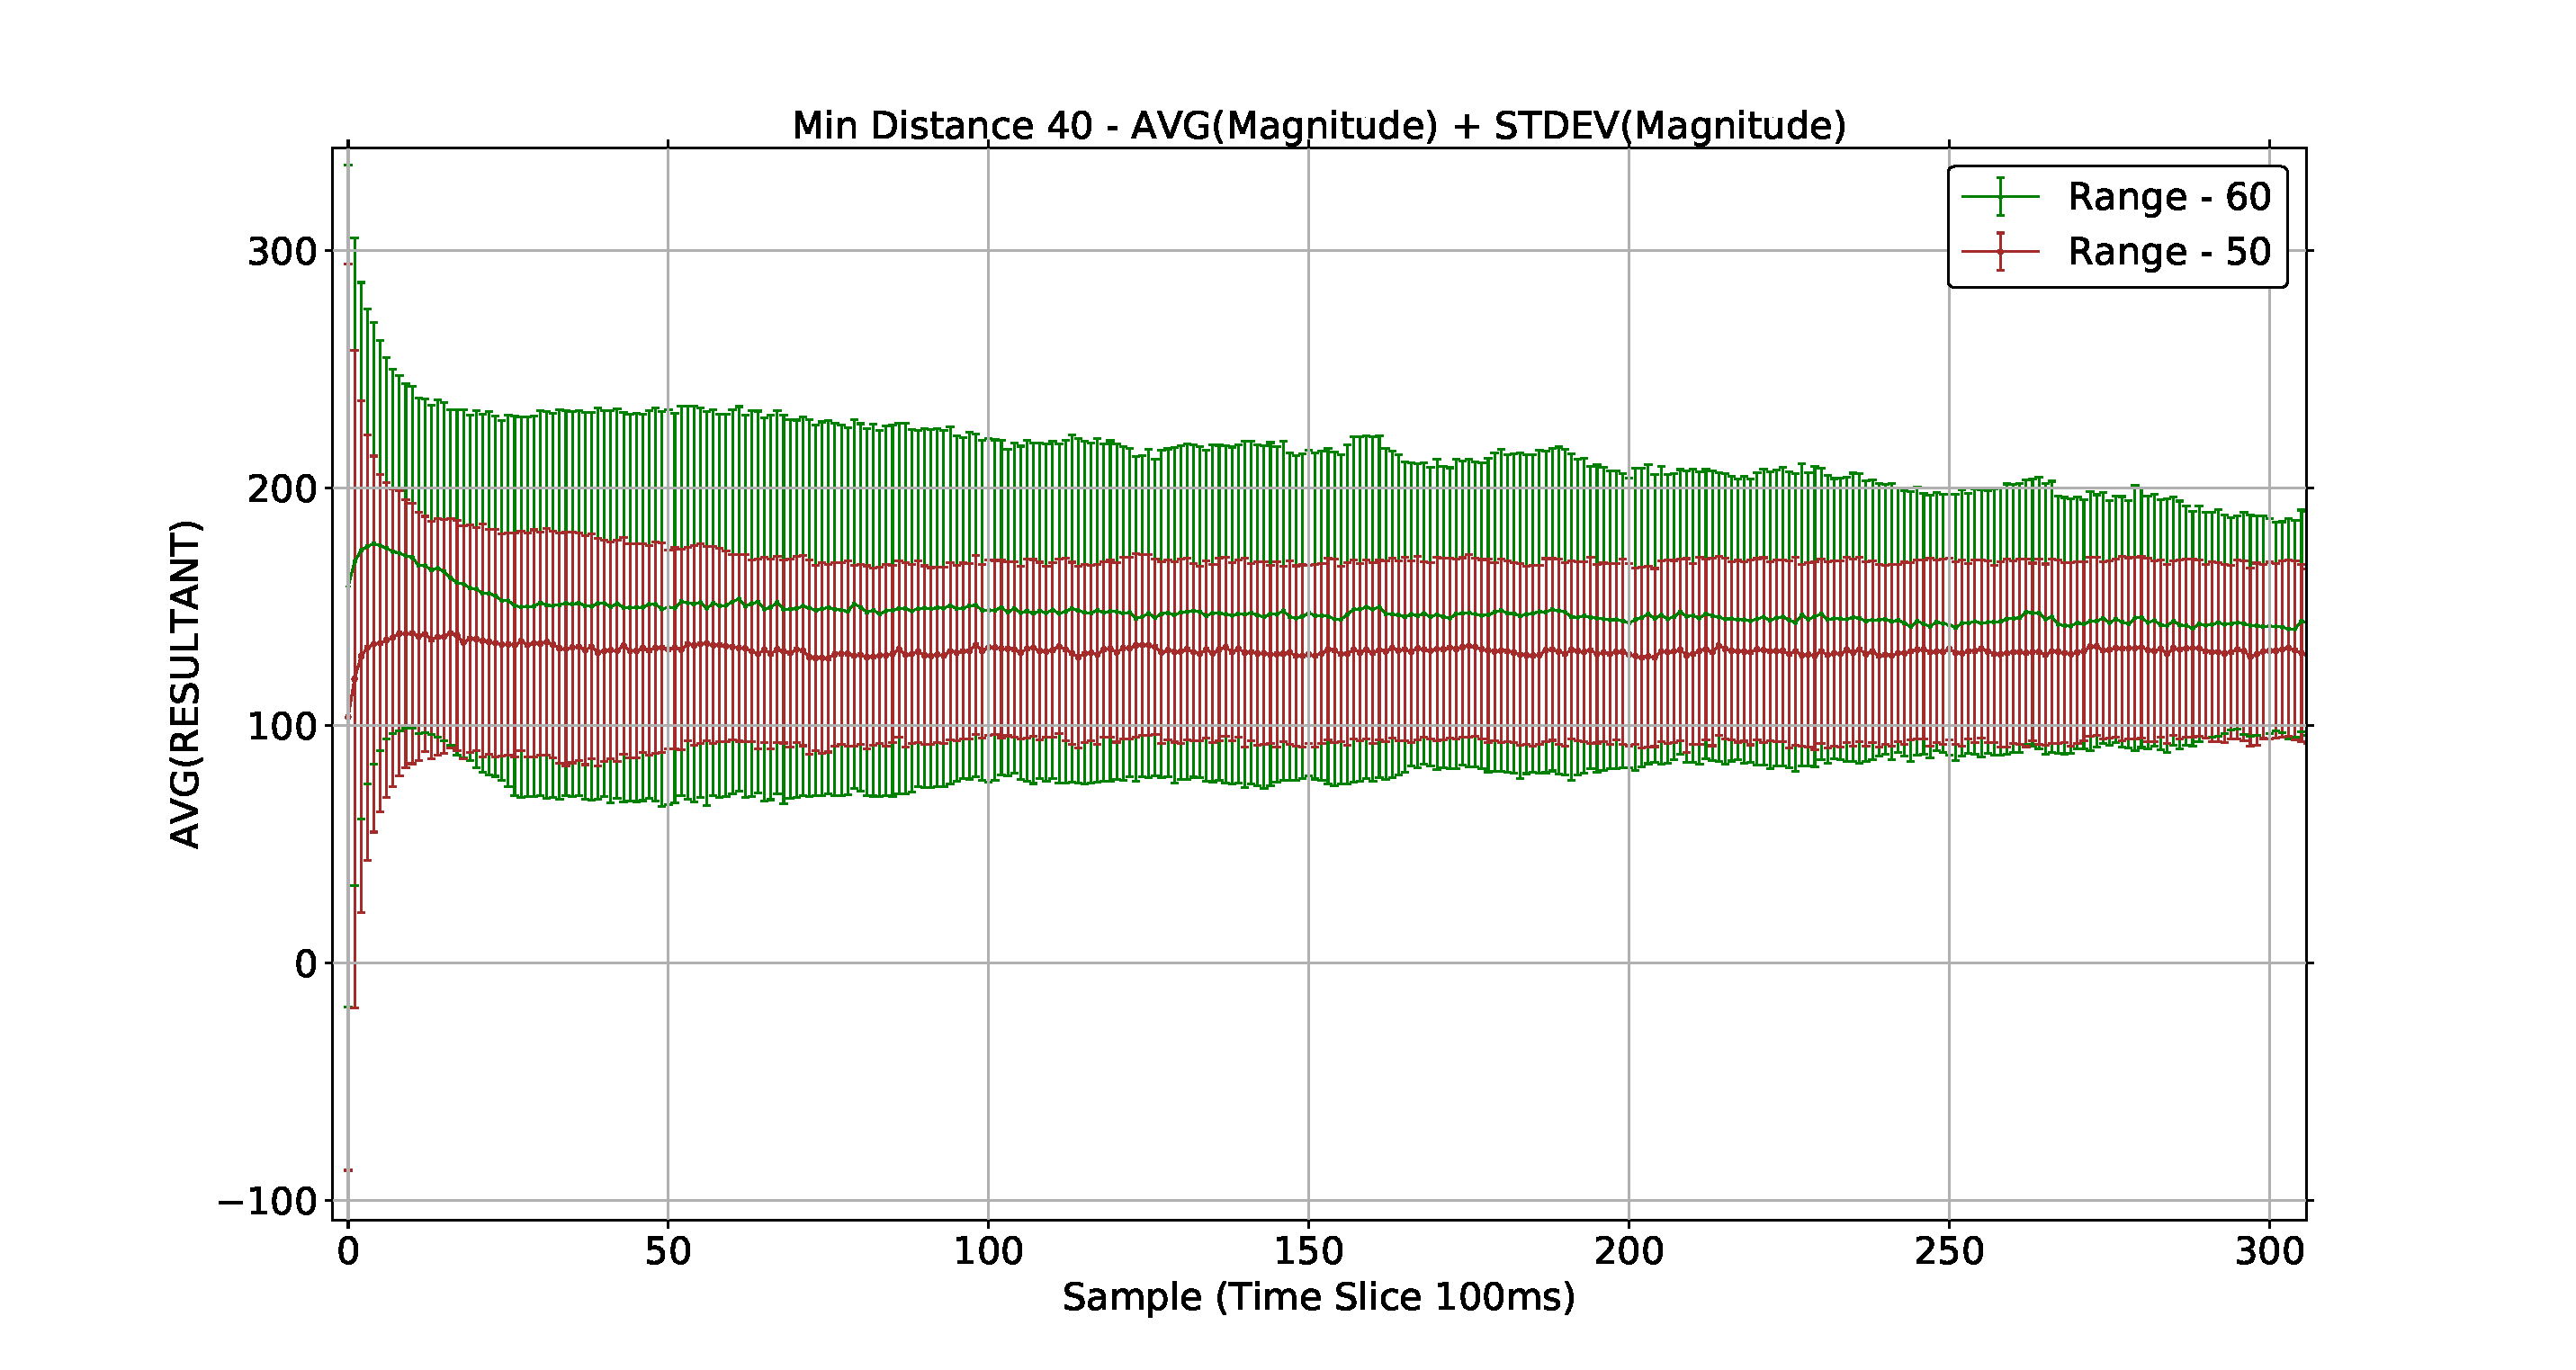
\includegraphics[width=13cm]{CHAPTER-5/figures/StabilityMagnitudeSwarm40-5060}
\end{center}
\caption{Agent resultant magnitude metric comparison\label{methods:StabilityMagnitudeSwarm40-5060}}
\end{figure}

A well structured and balanced swarm should therefore have a very low standard deviation in terms of the resultant metric~\autoref{methods:StabilityDistanceSwarm} and~\ref{methods:StabilityMagnitudeSwarm} clearly show using either magnitude or distance as the metric that the deviation from the mean can highlight the two different types of swarm when using the same repulsion field setting.
%HEX-HYPER-STD.py
\begin{figure}[H]
\begin{center}
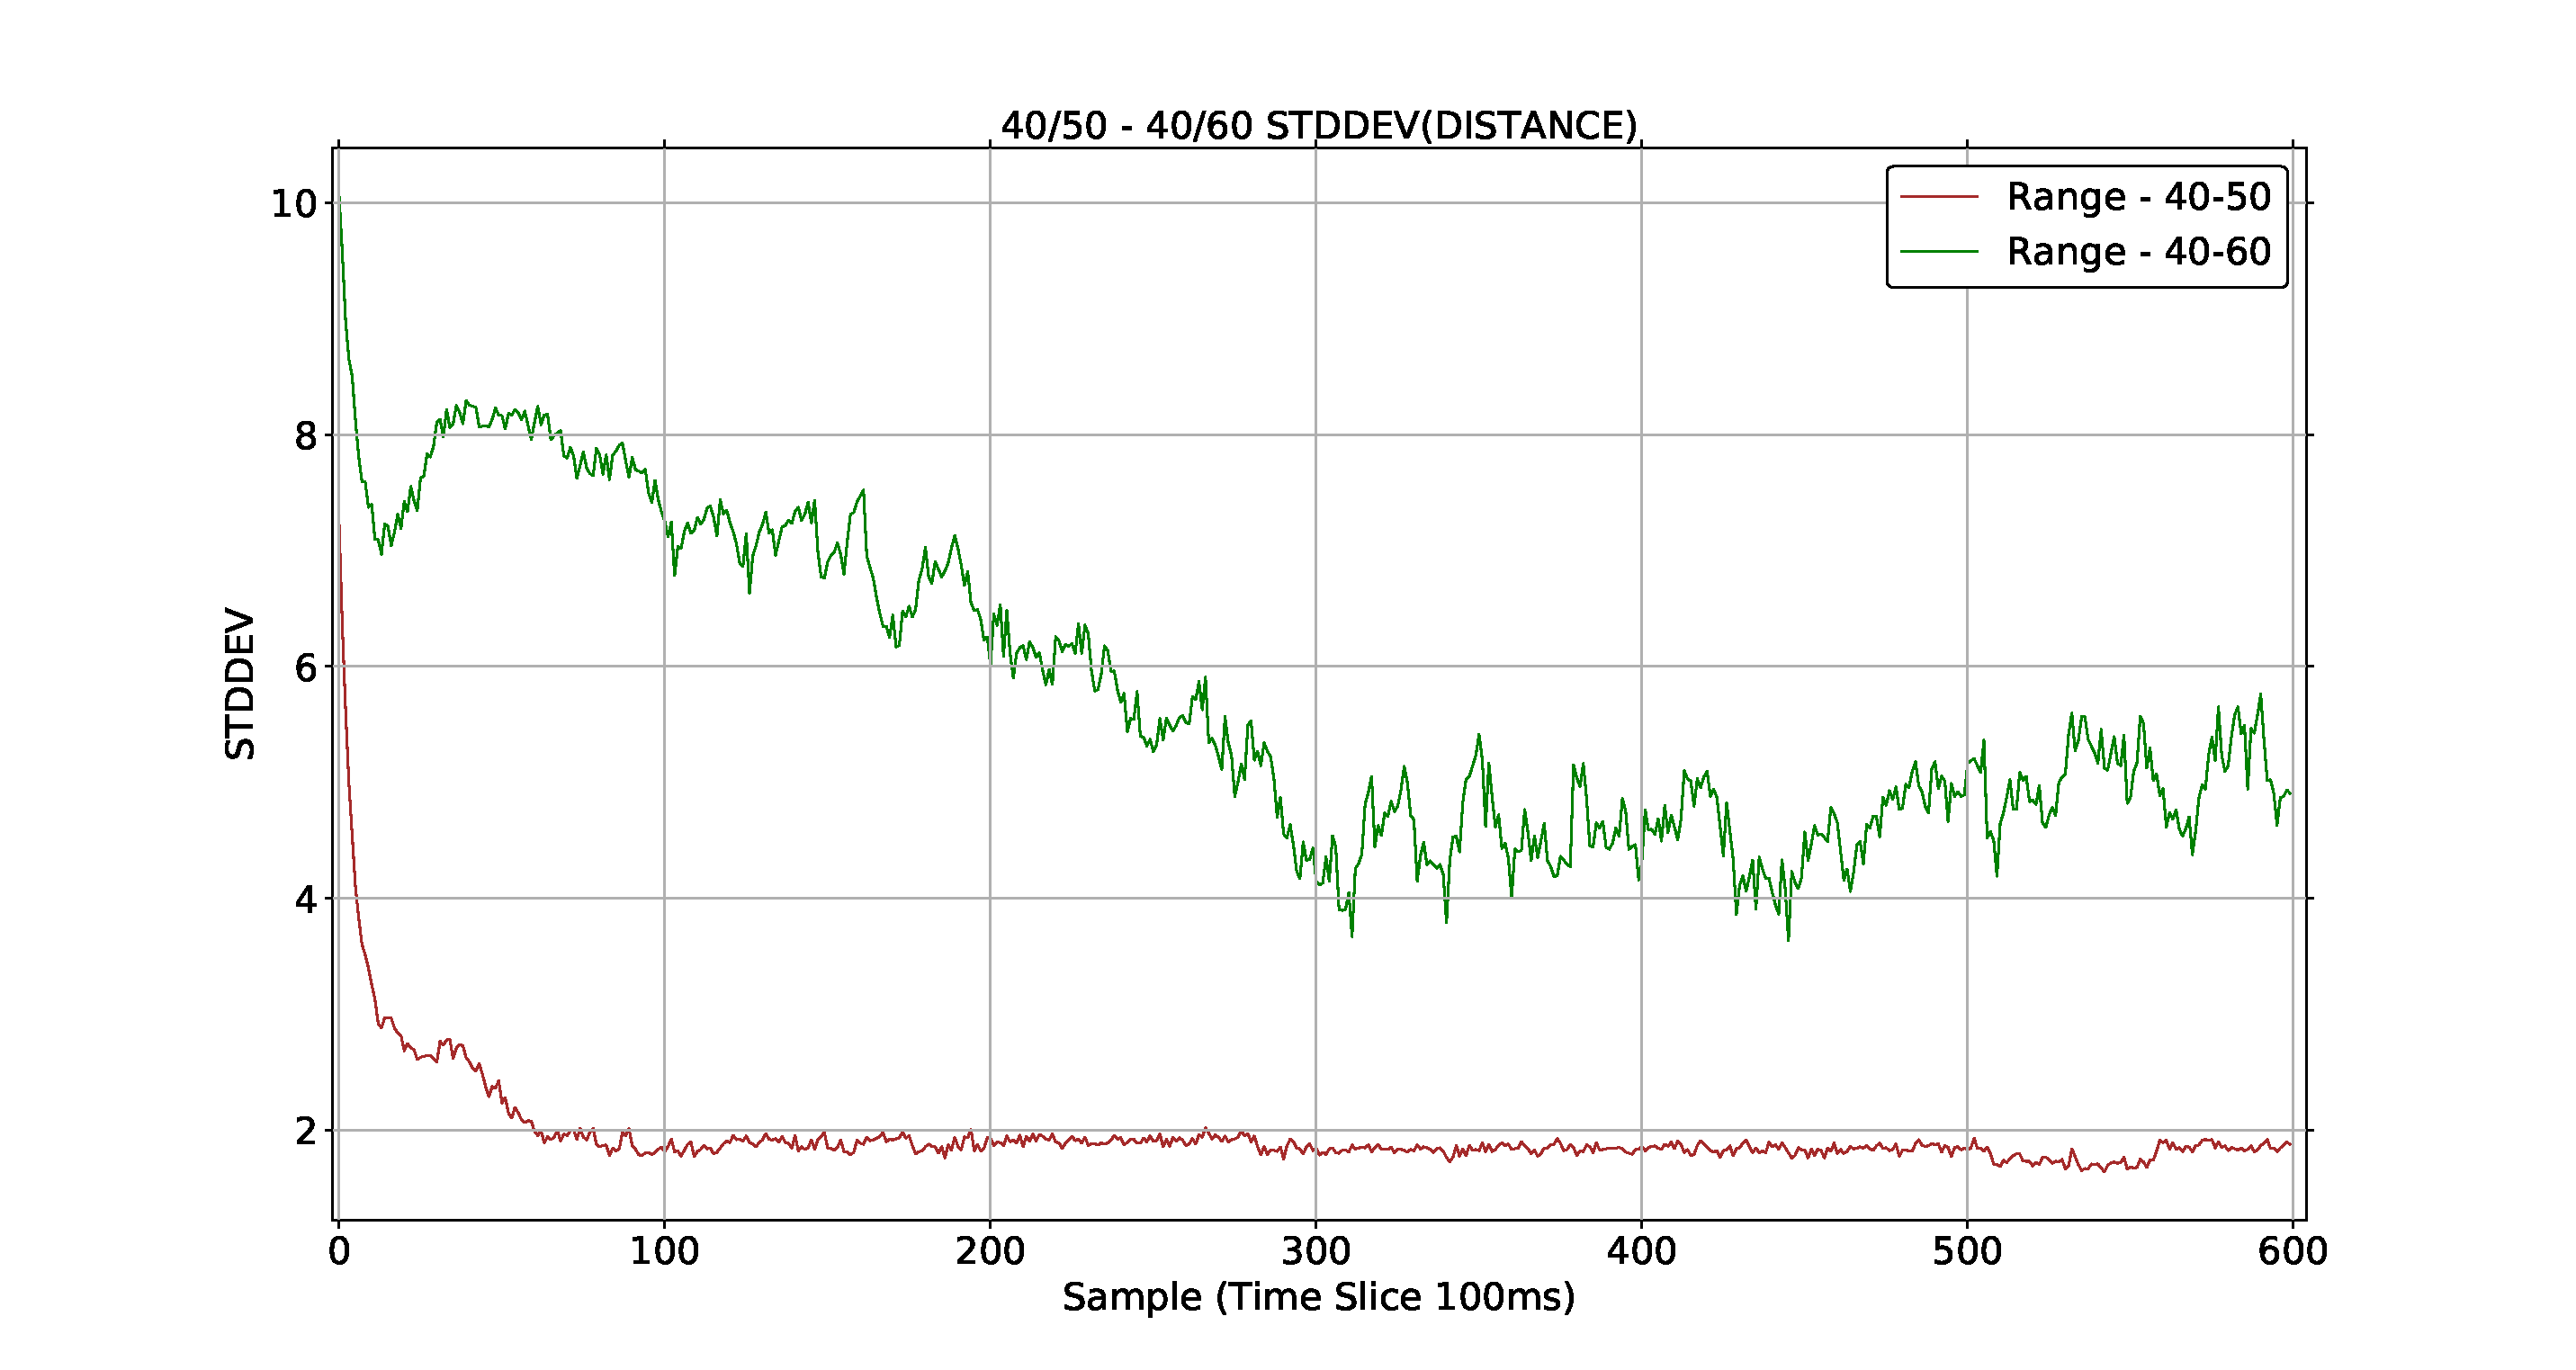
\includegraphics[width=13cm]{CHAPTER-5/figures/StabilityDistanceSwarm}
\end{center}
\caption{Distance based metric\label{methods:StabilityDistanceSwarm}}
\end{figure}
%HEX-HYPER-RES.py
\begin{figure}[H]
\begin{center}
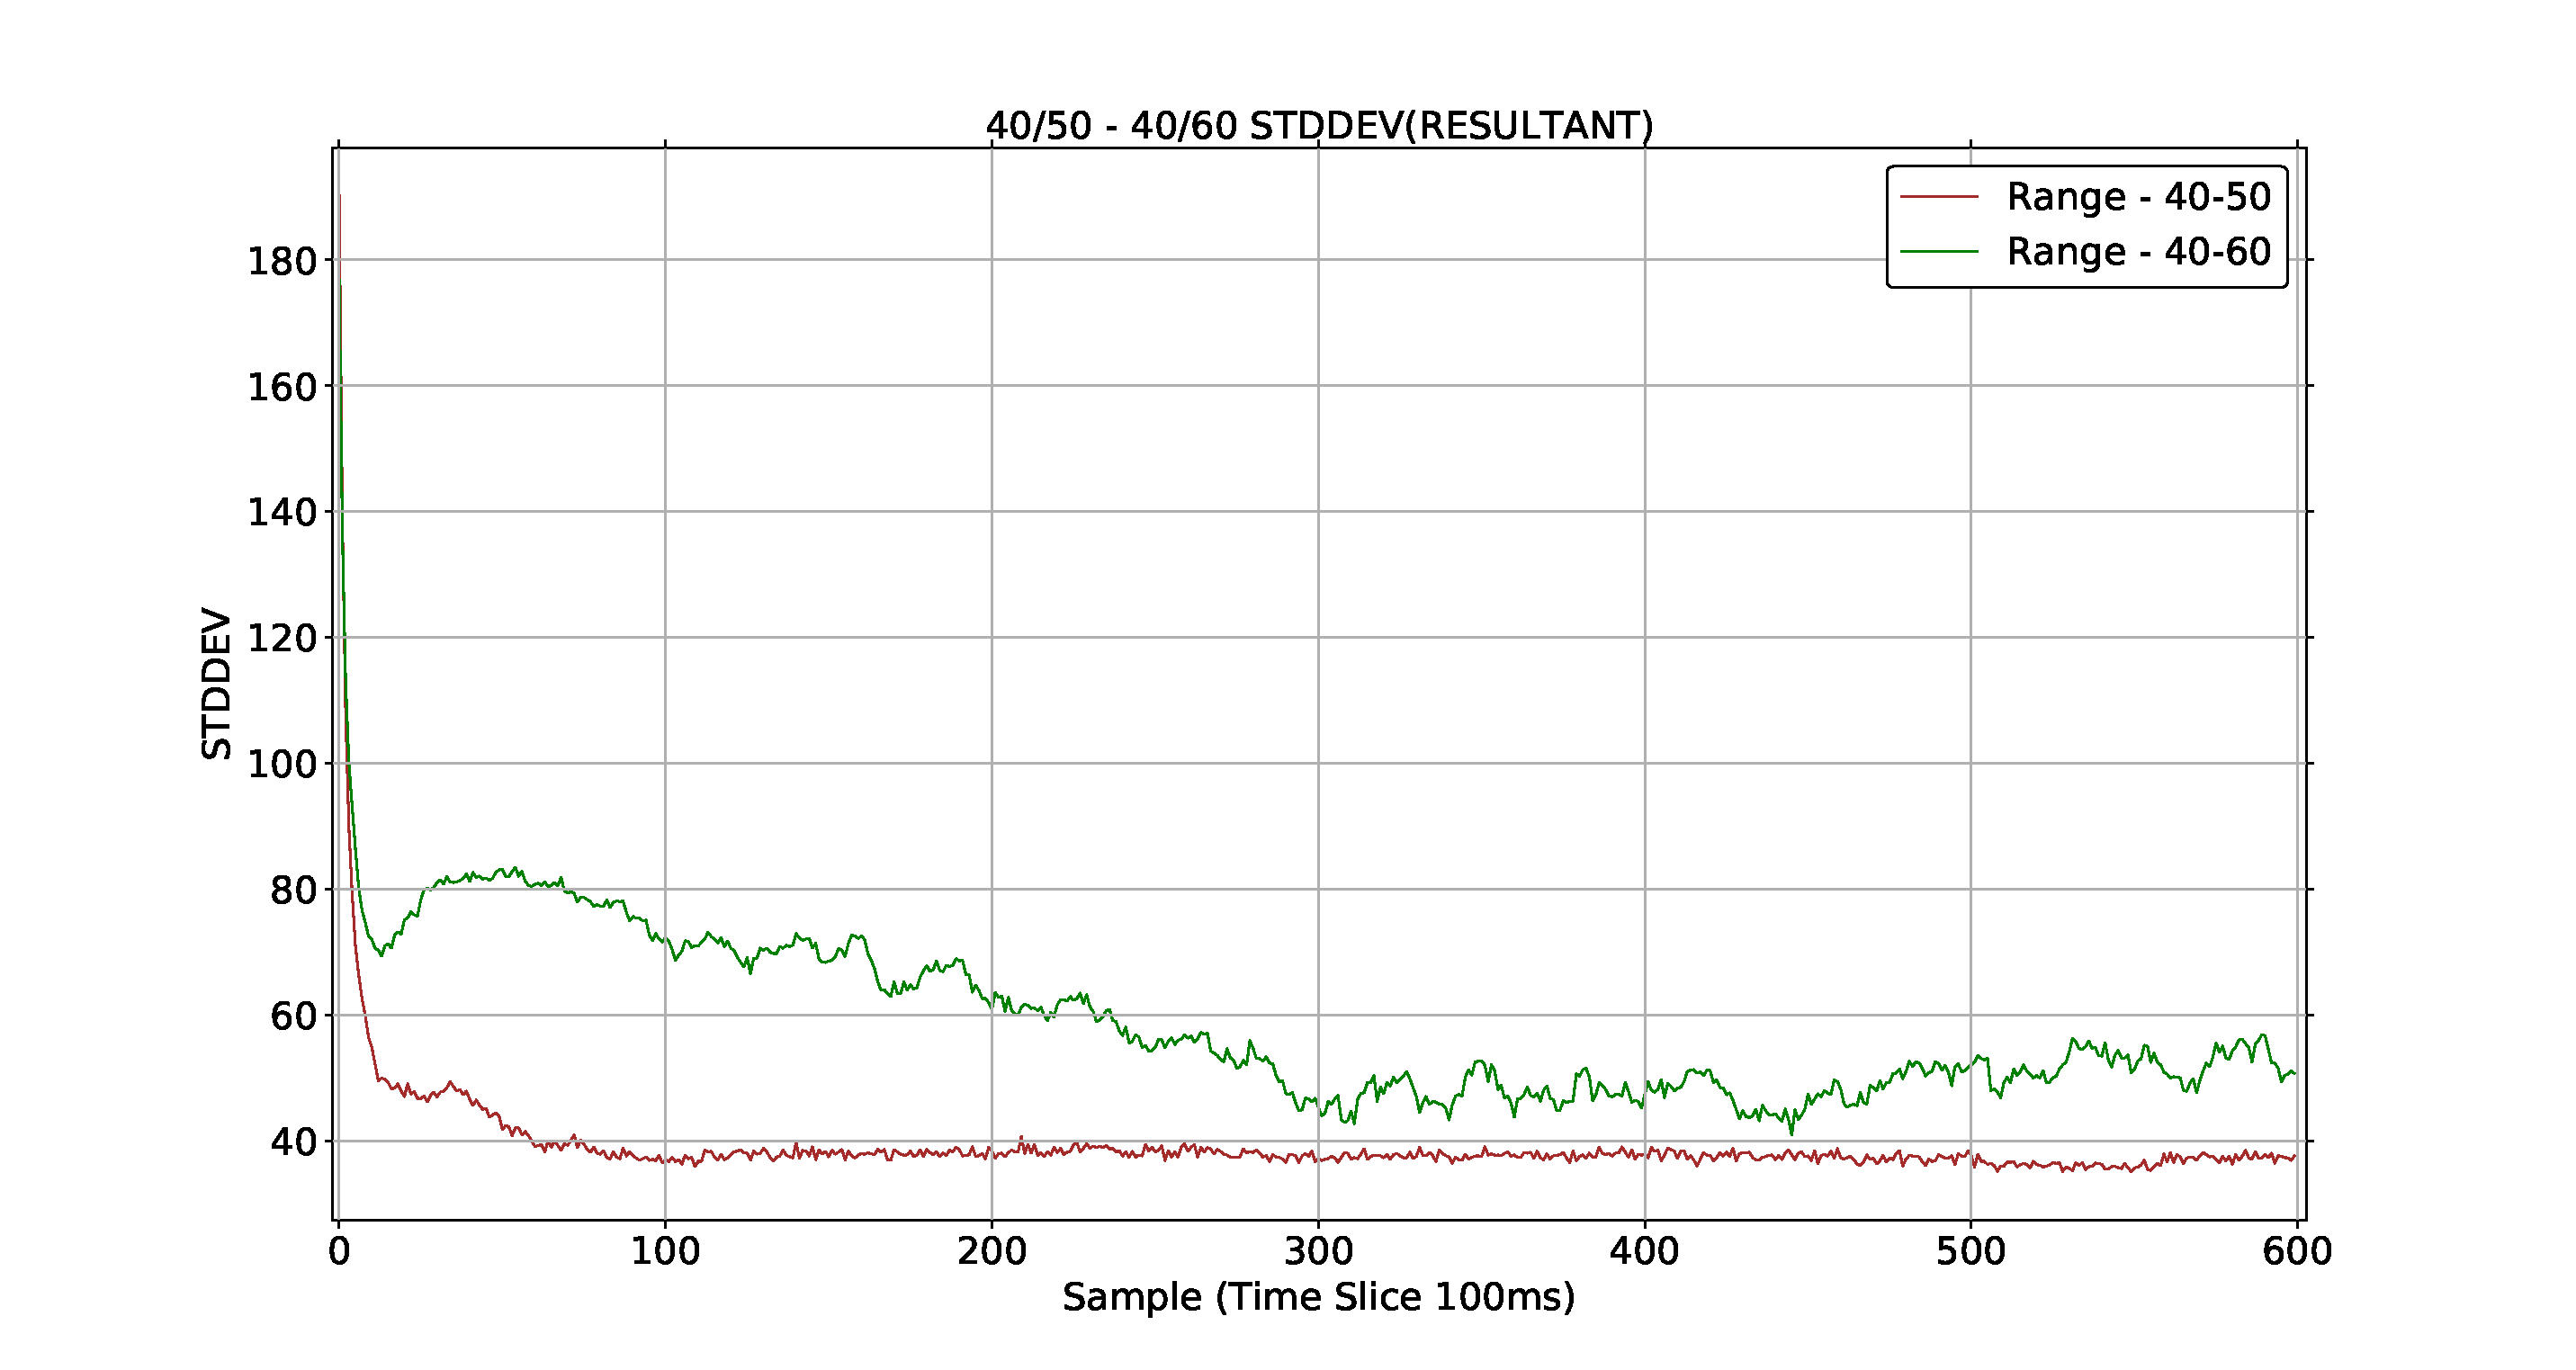
\includegraphics[width=13cm]{CHAPTER-5/figures/StabilityMagnitudeSwarm}
\end{center}
\caption{Agent resultant magnitude based metric\label{methods:StabilityMagnitudeSwarm}}
\end{figure}

The distribution of the agents over the entire simulation also shows it is possible to identify the mode of the swarm that is being generated by the cohesion field effect of the swarm. 
%HEX-HYPER-DIST-BAR.py
\begin{figure}[H]
\begin{center}
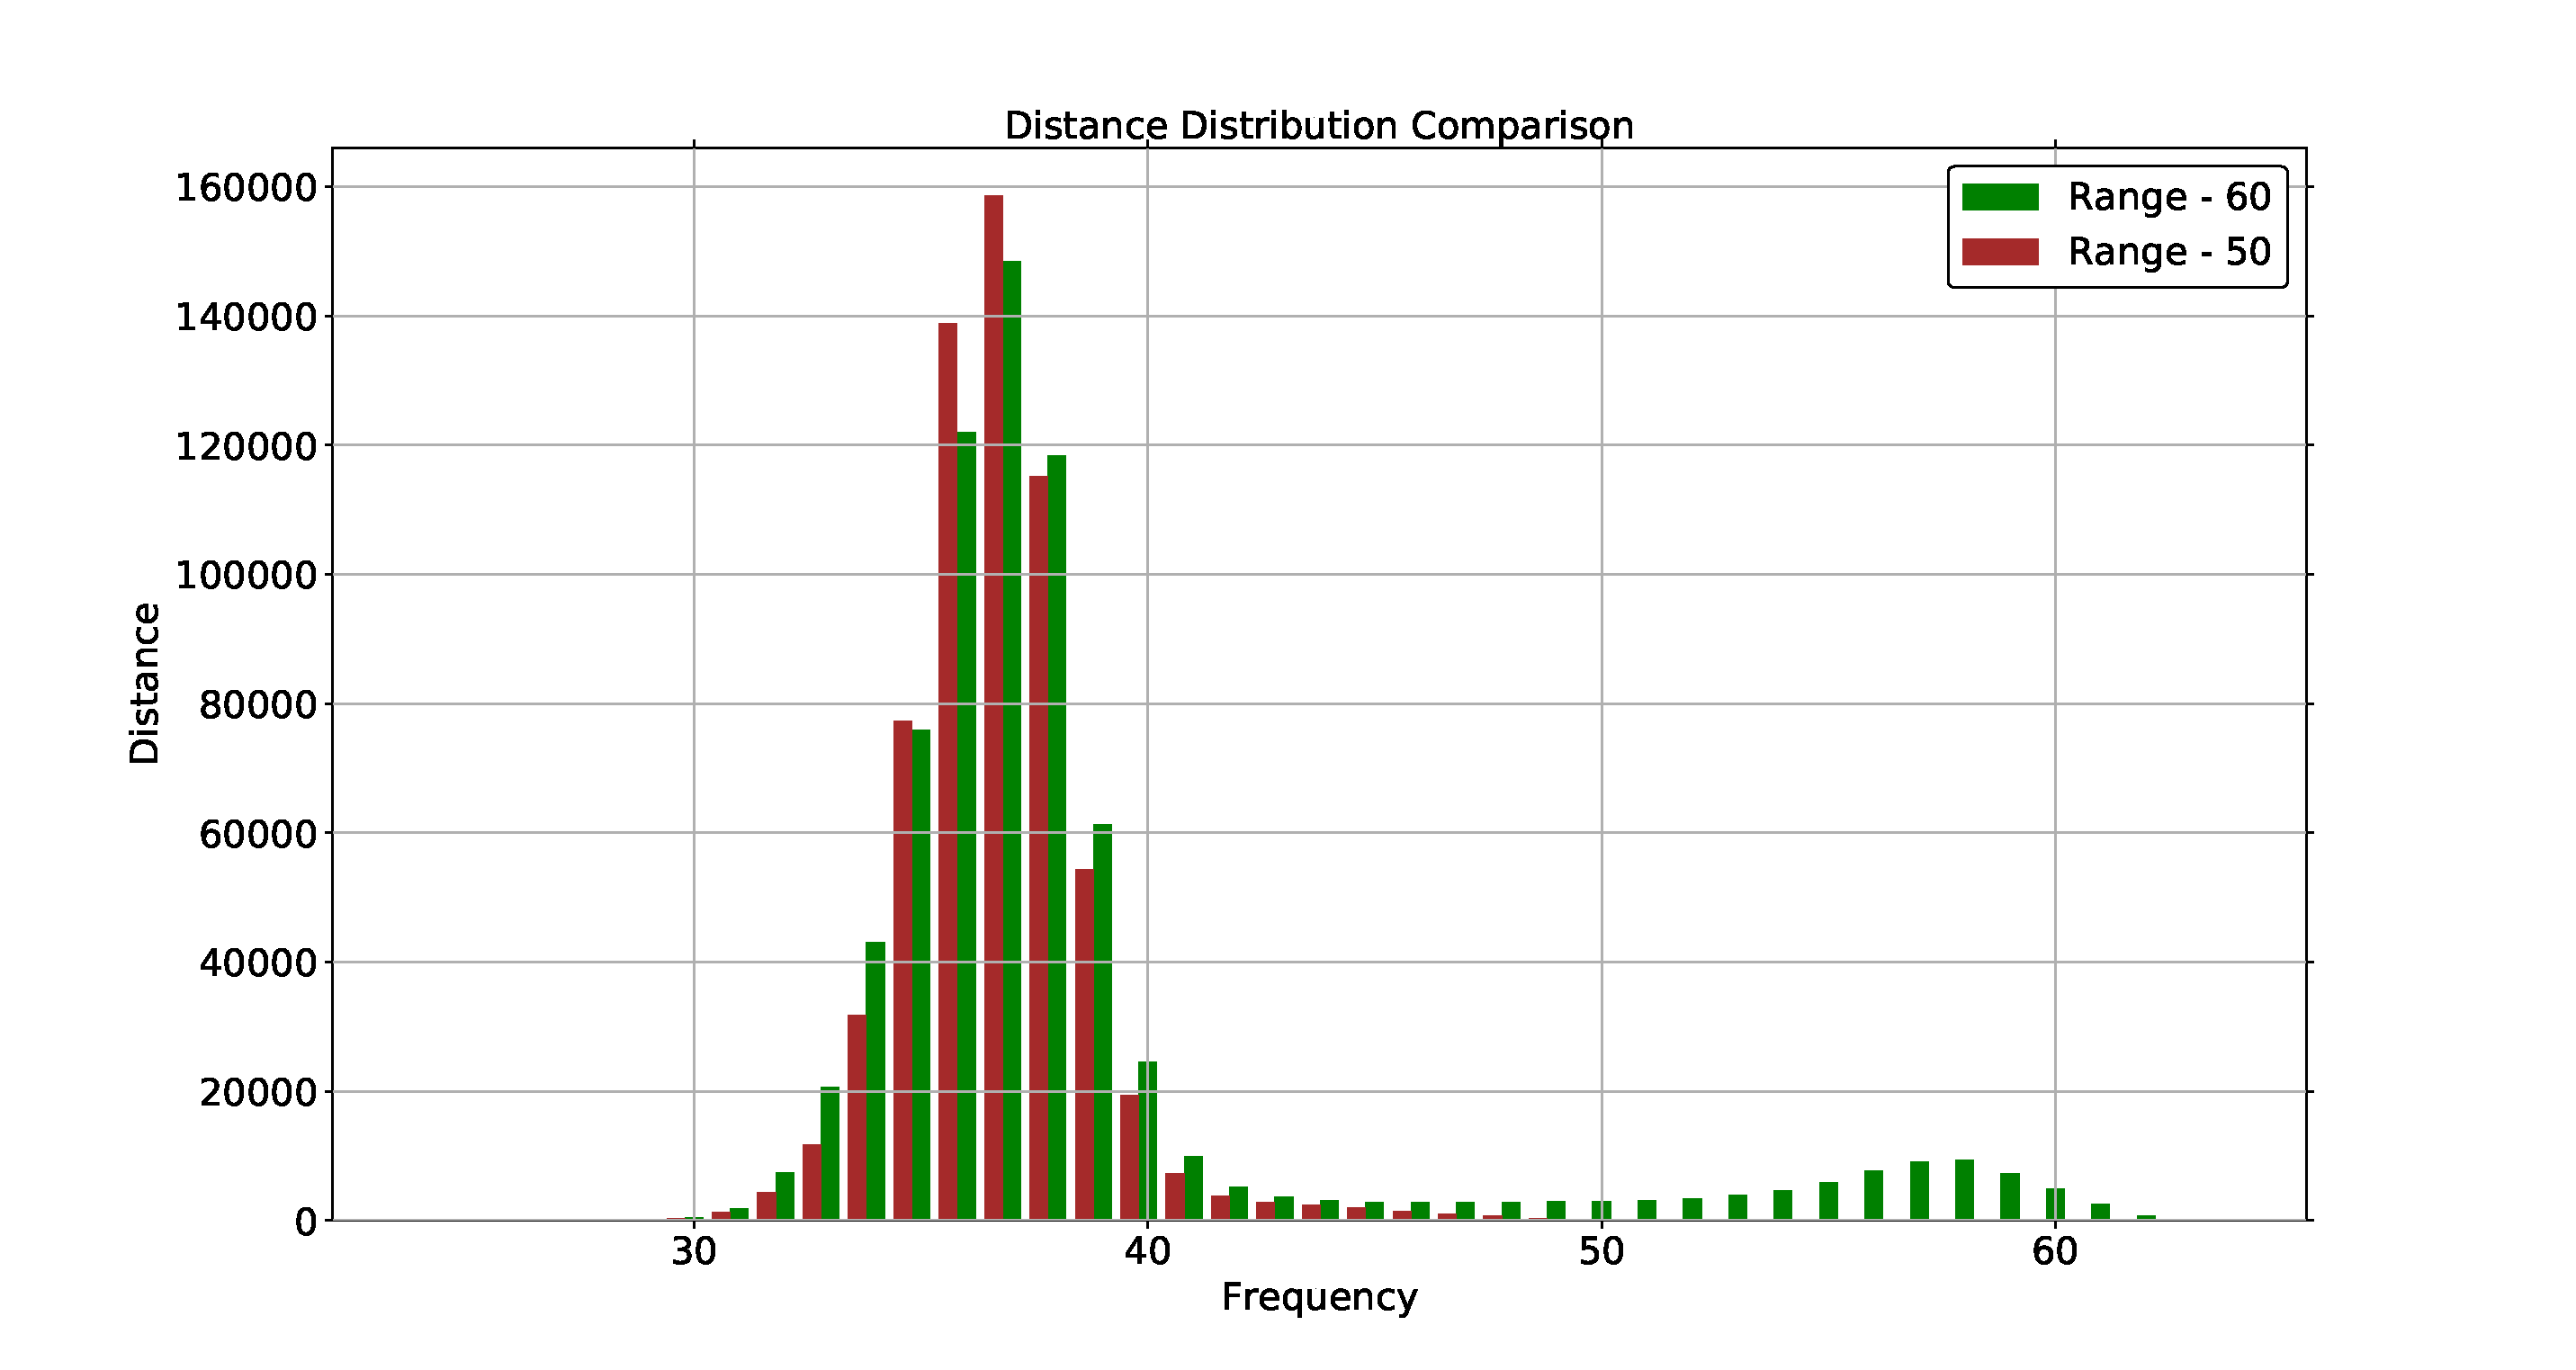
\includegraphics[width=13cm]{CHAPTER-5/figures/DistanceDistributionComparison}
\end{center}
\caption{Distance comparison\label{methods:DistanceDistributionComparison}}
\end{figure}

\autoref{methods:StabilityDistributionHyperHexagonal3D} and \ref{methods:StabilityDistributionHyperHexagonal3D2} show that over the duration of the simulation that the frequency of the mean for a hexagonal swarm is greater than that of the bi-model swarm. This is expected due to the additional vectors that are generated between agents. 
%HEX-HYPER-DIST-BAR-3D.py
\begin{figure}[H]
\begin{center}
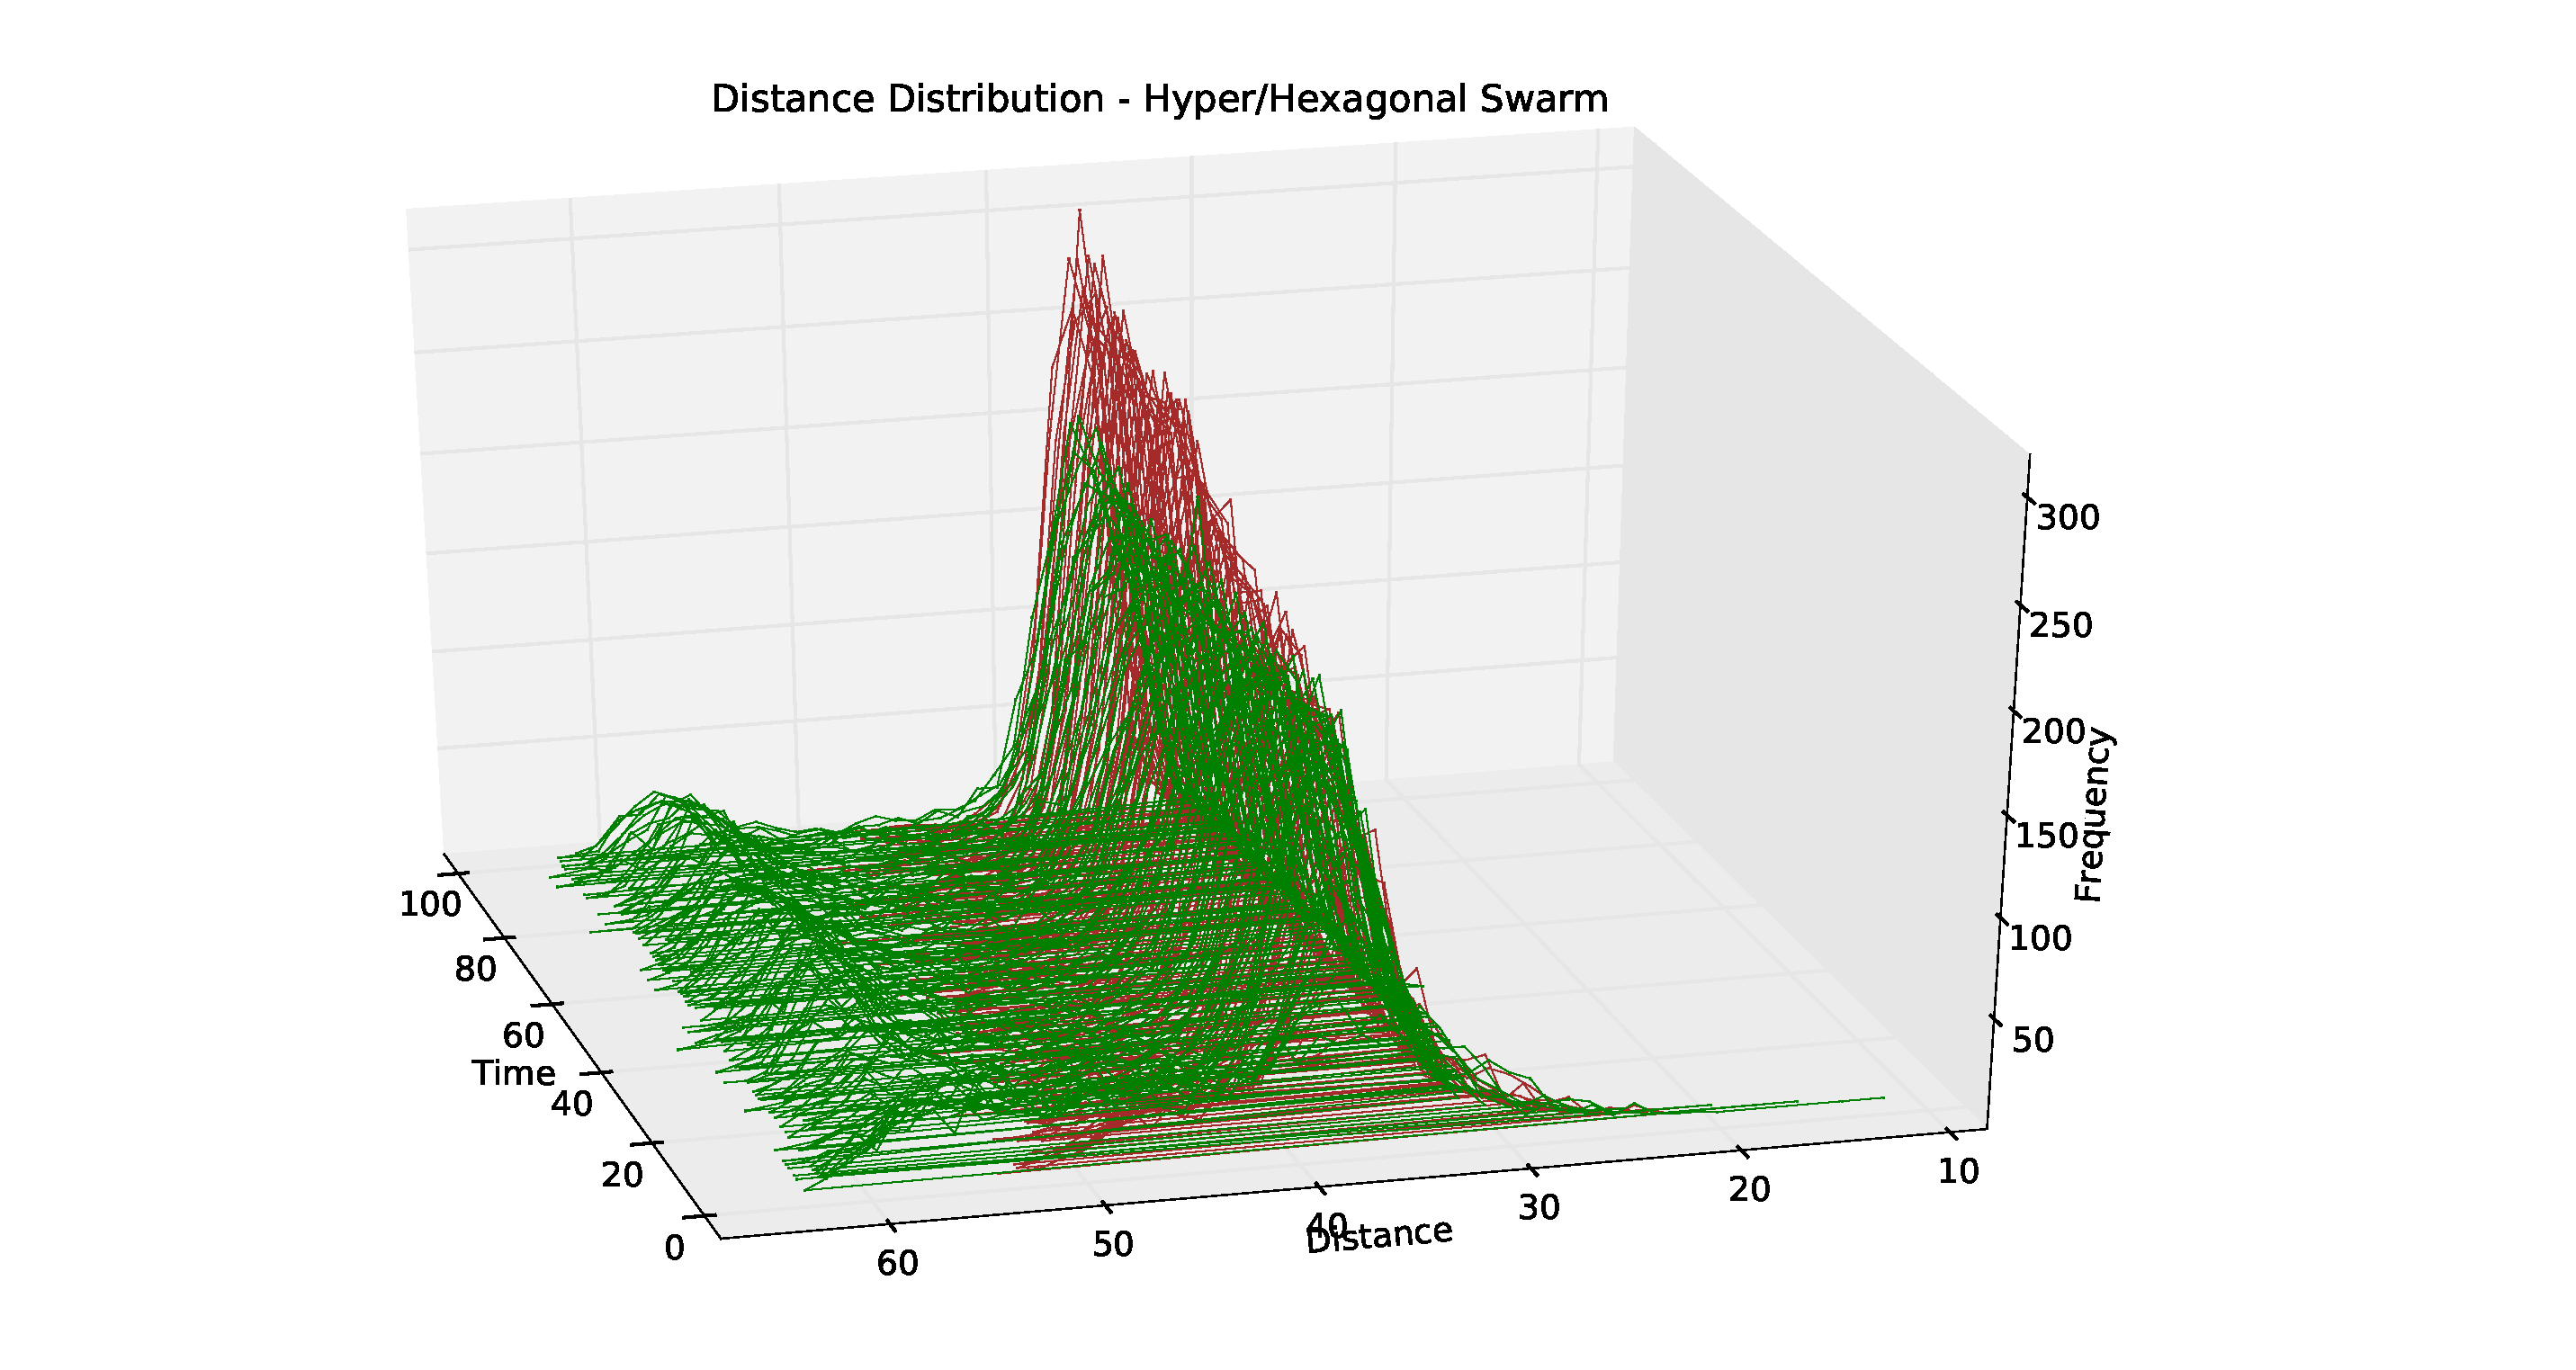
\includegraphics[width=13cm]{CHAPTER-5/figures/StabilityDistibutionHyperHexagonal3D}
\end{center}
\caption{Distance comparison / Time 0-10 seconds\label{methods:StabilityDistributionHyperHexagonal3D}}
\end{figure}
%HEX-HYPER-DIST-BAR-3D.py
\begin{figure}[H]
\begin{center}
\includegraphics[width=13cm]{CHAPTER-5/figures/StabilityDistibutionHyperHexagonal3D2}
\end{center}
\caption{Distance comparison / Time 10-0 seconds\label{methods:StabilityDistributionHyperHexagonal3D2}}
\end{figure}

\autoref{methods:MagnitudeDistributionComparison} shows that the mean magnitude potential for a hexagonal swarm is lower than that of the hyper-connected swarm.
%HEX-HYPER-MAG-BAR.py
\begin{figure}[H]
\begin{center}
\includegraphics[width=13cm]{CHAPTER-5/figures/MagnitudeDistributionComparison}
\end{center}
\caption{Agent resultant magnitude comparison\label{methods:MagnitudeDistributionComparison}}
\end{figure}

The most notable difference between the two magnitude metric analyses (\autoref{methods:StabilityMagHyperHexagonal3D} and \ref{methods:StabilityMagHyperHexagonal3D2}) is the initial potential magnitude of the hyper-connected swarm being greater than the hexagonal-swarm. This is due to the additional range of the field effect which generates a larger initial magnitude potential drawing the swarm together.
%HYPER-HEX-MAG-BAR-3D.py
\begin{figure}[H]
\begin{center}
\includegraphics[width=13cm]{CHAPTER-5/figures/StabilityMagHyperHexagonal3D}
\end{center}
\caption{Agent resultant magnitude comparison / Time 0-10 seconds\label{methods:StabilityMagHyperHexagonal3D}}
\end{figure}

\begin{figure}[H]
\begin{center}
\includegraphics[width=13cm]{CHAPTER-5/figures/StabilityMagHyperHexagonal3D2}
\end{center}
\caption{Agent resultant magnitude comparison / Time 10-0s\label{methods:StabilityMagHyperHexagonal3D2}}
\end{figure}

\section{Static swarm conclusion\label{section:staticConclusion}}
These results in terms of using magnitude or distance, provide similar profiles in terms of the changes in the profile of the plotted results. The distance metric discussed by Navarro~\cite{NIM:09} is used by many researchers that analyse agent distribution such as Cheein et al.~\cite{HGCTREA:15}, Bennet et al.~\cite{BM:09} and Barnes et al.~\cite{BAF:06, BAFVM:06, BFV:07, BFV:09}. Gazi et al.~\cite{GP:02, GP:04, GP:04a, GP:05} use this metric to analyse swarm stability. 

The similar profiles of the two metrics shows that either mechanism is suitable for identifying the internal movement within the swarm and providing a mechanism to compare the effects of swarming algorithms. The magnitude analysis, however, also provides a mechanism to determine if the swarm is expanding (a negative magnitude) or cohesive (a positive magnitude).

The metrics both provide an ability to adjust the variable parameters of the swarming mechanics (cohesion, repulsion and direction) or the range of the neighbour detection and minimum proximity distances and to identify the effect that those changes have upon the swarm in terms of the swarms internal movement. If we consider the internal movement to be a measure of the quality of a swarm in a given situation then these measures are identifying the swarming algorithms effectiveness.

\subsection{Arbitrary sized swarms}\label{section:arbitrary}
This thesis if focused on arbitrary sized swarms. The algorithms that are used only require localised sensing which therefore all movement and positioning calculations are based on neighbours. As localised data is used it should be possible for the algorithms to be effective with swarms of any size. The swarms configuration in this section is based upon a swarm of 200 agents but the application of the field effects coordination will work with larger swarms. \autoref{methods:ArbitrarySize200500} shows a comparison the distance metric of swarms of 200 and 500 agents and \autoref{methods:ArbitrarySizeMag200500} shows a comparison of the Magnitudes.

\begin{figure}[H]
\begin{center}
\includegraphics[width=13cm]{CHAPTER-5/figures/ArbitrarySize200500}
\end{center}
\caption{Swarm size distance comparison\label{methods:ArbitrarySize200500}}
\end{figure}

\autoref{methods:ArbitrarySize200500} shows the average distance of the agents fluctuate while the swarm stabalises (disorganised stage) and eventually both swarms stabalise to comparable distances and variations. 

\begin{figure}[H]
\begin{center}
\includegraphics[width=13cm]{CHAPTER-5/figures/ArbitrarySize200500MAG}
\end{center}
\caption{Swarm size magnitude comparison\label{methods:ArbitrarySizeMag200500}}
\end{figure}

\autoref{methods:ArbitrarySizeMag200500} shows the average magnitude of the agents fluctuate while the swarm stabalises (disorganised stage) and eventually both swarms stabalise to comparable magnitudes and variations.

These two metrics show that the swarm is able to expand to its maximum distribution without being impeded. If the swarms area was impeded the magnitude would not have been able to stabalise and would have remained high. The identification of swarm bound containment will be discussed in chapter~\ref{chapter:flooding}.

%% \subsection{Mobile swarm internal movement testing\label{section:swarmTesting}}
%% The results presented here show that the metric will identify changes in a swarm, this metric can therefore be applied to measure the resulting internal movement of the swarm when it is goal based. The metrics can also be used to identify the effects of negotiating obstacles or modifications to an algorithm to exploit a behaviour such as closing voids or surround an object.
%% 
%% With a stationary swarm the only influencing factors that need to be taken into consideration are the cohesion and repulsion of the agents. The most obvious change to the swarms algorithm is to include a directional bias. The most common way of applying the bias is to include a GPS sensor into each of the agents to provide a direction that is then used to apply a directional influence to the swarm. 
%% 


  %contribution 3
\chapter{Swarm coordination - perimeter detection}\label{chapter:coordination}
%% \section{Introduction}
This chapter identifies the effect a \textit{destination vector} has upon the motion of a swarm. Three coordination techniques are applied to a swarm and the metrics defined in chapter~\ref{chapter:metric} are used to identify the effects. The three coordination techniques are: full perimeter detection, where only edge based agents will have a \textit{destination vector} applied partial perimeter detection, where a subset of the perimeter agents are detected and finally all agents in the swarm having a \textit{destination vector} applied. For all the experiments the base parameters of the swarm are fixed ensuring that the only variable will be the \textit{destination vector} that is applied by the coordinating agents. This process allows the impact of the algorithms to be isolated and compared. Section~\ref{sec:AlternateBias1}~discusses the potential variations to the base parameters and the effects this has on controlling the impact of the weightings.

\section{Baseline specification}
To allow an analysis of each algorithm's effect on a swarm a baseline measurement of `background' variance (jitter) is identified. The baseline measurement provides a comparative data set for the experiments. The baseline data set is for a static swarm (no destination vector) with the same internal parameters.

\textit{Assumption 1:} The swarm used for the experiments consists of 200 agents randomly distributed~(Figure~\ref{fig:SampleSwarm200-1}).\\ 
\textit{Assumption 2:} The field effects and bias will be set as shown in~Table~\ref{tab:DynamicPhysics1} with the weight adjuster $k_d = 0$ for the baseline.\\
\textit{Assumption 3:} All destination based experiments will have the weight adjuster set to $k_d = 100$.

\begin{figure}[H]
\begin{center}
\includegraphics[width=14cm]{CHAPTER-6/figures/SampleSwarm200-1}
\end{center}
\caption[Sample swarm 200 agents initial state]{Sample swarm 200 agents initial state (\textit{screen shot from simulator})\label{fig:SampleSwarm200-1}}
\end{figure}

\begin{table}[H]
\begin{center}
\begin{tabular}{| p{2.5cm} | c | p{7cm} |}
\hline
\bf Weight \bf Component & \bf \swarmA{} & \bf Description \\ \hline
Sample Rate & 100 & ms - Unit sampling interval\\  \hline
$k_c$ & 5 & weight adjuster for cohesion vector\\  \hline
$k_r$ & 15 & weight adjuster for repulsion  vector\\  \hline
$k_d$ & 0/100 & weight adjuster for destination vector 0 for static baseline 100 for destination based\\  \hline
Repulsion field & 70 & units\\  \hline
Cohesion field & 80 & units\\  \hline
Speed & 20 & units/s\\  \hline
\end{tabular}\caption{Swarm Weighted Model} \label{tab:DynamicPhysics1}
\end{center}
\end{table}

The results for the baseline experimental swarm are shown in~Table~\ref{coord:BaselineMagnitude1} and~\ref{coord:BaselineDistance1}. The metrics used are the distance \cite{NIM:09} and resultant inter-agent magnitudes (\textit{inter-agent vector}).

\begin{figure}[H]
\begin{center}
\includegraphics[width=14cm]{CHAPTER-6/figures/BaselineMagnitude1}
\end{center}
\caption{Baseline internal movement - magnitude\label{coord:BaselineMagnitude1}}
\end{figure}

Figure~\ref{coord:BaselineMagnitude1} shows the magnitude between $t_0$ and approximately $t_{48}$ dominated by repulsion ($|k_rv_r| > |k_cv_c|$). This indicates that the swarm is undergoing a rapid expansion as the bias within the swarm shows a high level of repulsion. Between approximately $t_{48}$ and $t_{100}$ the magnitude is positive but rising which indicates the swarm is cohesive and will remain a cohesive unit but it is still expanding. At approximately $t_{110}$ the swarm has completed it's expansion and has reached a settled state with the `background' movement maintaining the swarm's structure with $|k_rv_r| < |k_cv_c|$. The residual `jitter' is at its minimum for the configuration and the agent distribution is at its optimum for the cohesion and repulsion settings. The resultant $|k_rv_r| < |k_cv_c|$ is due to the cohesion field being larger than the repulsion field which prevents the swarm `breaking up'. 

\begin{figure}[H]
\begin{center}
\includegraphics[width=14cm]{CHAPTER-6/figures/BaselineDistance1}
\end{center}
\caption{Baseline internal movement - distance\label{coord:BaselineDistance1}}
\end{figure}

Figure~\ref{coord:BaselineDistance1} shows the internal movement and the deviation from the mean for the swarm based on the inter-agent distances. There is no \textit{destination vector} applied so all internal movement is being generated by the cohesion and repulsion vectors. The swarm is initially in a disorganised state but once the agents have expanded a stable hexagonal formation evolves. Figure~\ref{coord:BaselineDistance1} shows the first 30s of the simulation which is sufficient time for the swarm to `settle' and transform to its most stable state. Due to the metric only showing inter-agent distances it is not possible to determine if the swarm will remain cohesive.

The centroid path for the baseline swarm is shown in~Figure~\ref{coord:SwarmPathBaseline1}. Due to there being no \textit{destination vector} for the swarm the centroid changes positions based on the inter-agent positional changes caused by the \textit{interaction vectors}. These changes are the result of each agents attempting to attain a state of equilibrium within their `clusters'.

\begin{figure}[H]
\begin{center}
\includegraphics[width=14cm]{CHAPTER-6/figures/SwarmPathBaseline}
\end{center}
\caption{Baseline swarm path\label{coord:SwarmPathBaseline1}}
\end{figure}

These baseline measurements are used to identify the changes that occur in the structure of a swarm when changes are made to the weightings of the field effects, the number of coordination agents and the \textit{destination vector} weighting.

\section{Destination vector application}
Many mechanisms can be used to influence a swarm to travel in a specific direction. These mechanisms generally involve the use of sensors such as magnetometers or GPS's to achieve a directional coordinate \cite{SG:15,TG:12}. 

This thesis aims to produce algorithms that will reduce the number of active sensors that are needed for the directional coordination of a swarm. When reducing the number of active sensors the algorithms must maintain sufficient coordination of agents to influence the swarm's direction and therefore create an overall \textit{destination vector} to a swarms movement. Reducing the number of active sensors will reduce the net energy usage of the sensors and potentially increase the sensors viable lifetime. Another aspect of the algorithms is that they should minimise the internal disturbance (jitter) created by the \textit{destination vector}.

There are two distinct approaches to configuring agents: all the agents are configured identically (homogeneous swarm) or the agents are in a selection of different configurations (heterogeneous swarm)~\cite{BS:13}. 

The following assumptions are made in this thesis:

\textit{Assumption 1:} All agents are identical (homogeneous) but are able select subsystems as necessary and adopt different roles depending upon the algorithm being used to coordinate the swarm. \\
\textit{Assumption 2:} As the swarm progresses towards a destination the role of an agent can change such that all the agents are identical in construct but they can enable and disable sensors as necessary. This will allow agents within the swarm to self promote to the coordinator role should a set of conditions arise.\\
\textit{Assumption 3:} All agent in the swarm are autonomous and each agent has its own power supply. 

Reducing the usage of sensors will reduce the net power consumption of the swarm and increase the time that an agent can be a part of a swarm. If the purpose of the swarm is reconnaissance then the reduction in energy usage may allow a longer traversal time, or allow the swarm to travel further. As agents in the swarm will use their resources at different rates some agents may be lost due to resource exhaustion. The algorithms should therefore be resilient to this.

\section{Swarm destination vector}
The following assumptions are made in this thesis:

\textit{Assumption 1:} The direction of the swarm is based upon having a fixed goal that is known to all the agents (Section~\ref{sec:Direction1}). \\
\textit{Assumption 2:} The goal is migrated towards based on a simulated GPS signal and the bias $k_d$ is applied to the \textit{destination vector} to influence the movement of the agents. 

The swarm's destination is established by the coordinator agents influencing the non-coordinator agents. This influence is applied through the coordinators proximity to non-coordinator agents (cohesion). Coordinator agents are identified by a set of conditions. The conditions are the activators for the coordinator identification algorithms.

\section{Identifying the coordinator role}
For an agent to change its role from a standard agent to a coordinator there needs to an algorithm that identifies a set of conditions to trigger the change. This same algorithm also triggers an agent to revert to being a standard agent. The coordinator selection algorithm is separate from the agent coordination algorithms discussed in chapter~\ref{chapter:methods}.

In this thesis three algorithms are presented and compared. In the first algorithm, all agents have the role of a coordinator permanently. This will be referred to as the all-agent algorithm. The other two mechanisms employ a selection criteria to identify if the simulated GPS sensor should be enabled. These two algorithms are: full-perimeter detection and the partial perimeter detection. Partial perimeter detection will be referred to as the basic-count algorithm.

There are many other ways in which the coordinator role could be established such as randomly enabling a GPS for a set period of time or oscillating the role on and off but they are beyond the scope of this thesis.

\section{Monolithic swarm - (all-agent)} 
In a monolithic swarm \cite{BS:13} the propagation towards the goal is achieved by all the agents using a GPS signal to give each agents' movement a \textit{direction vector} towards a required goal~(Equation~\ref{eq:BotDirection1}). There is no selection criteria and no computational overhead for the agents.

Figure~\ref{reduced:Monolithic1} shows a screen shot from the swarm simulator with all agents GPS's enabled. This can be seen as the agents highlighted with a ring around them. The small `tail' on each agent is the \textit{movement vector}.

\begin{figure}[H]
\begin{center}
\includegraphics[width=7cm]{CHAPTER-6/figures/Monolithic2}
\end{center}
\caption[Monolithic agents]{Monolithic agents (Circles indicate all agents are using GPS, \textit{screen shot from simulator}) \label{reduced:Monolithic1}}
\end{figure}

\subsection{Baseline and effect of no perimeter detection\label{section:compareBaselineNoPerimeter}}
To identify the effect of the all-agents algorithm the simulation is executed using the same parameters as the baseline swarm with the added \textit{destination vector} on all the agents. The effect of introducing this bias on the swarms internal characteristics can be seen in~Figures~\ref{reduced:BaselineAllAgentsMag1} and~\ref{reduced:BaselineAllAgentsDist1}.
%BASELINE-ALLAGENTS-MAG.py
\begin{figure}[H]
\begin{center}
\includegraphics[width=14cm]{CHAPTER-6/figures/BaselineAllAgentsMag1}
\end{center}
\caption{Baseline/All agents comparison \textit{inter-agent vector} magnitude\label{reduced:BaselineAllAgentsMag1}}
\end{figure}

Figure~\ref{reduced:BaselineAllAgentsMag1} shows the effect on the \textit{inter-agent vector} magnitude of the swarm: the average resultant magnitude is lower than the baseline. This is due to there being a greater distribution of \textit{inter-agent vector} magnitudes from the disturbance caused by the \textit{destination vector} on all of the agents and the swarm is therefore less cohesive. The graph also shows that there is a higher variation from the mean; again this is due to the change in the bias of all the agents. The agents are moving towards a goal and are therefore not moving to an equilibrium distribution. Figure~\ref{reduced:BaselineAllAgentsMag1}~also shows that the \textit{direction vector} increases the time it takes for the swarm to distribute the agents and although the deviation diminishes the swarm cannot overcome the \textit{direction vector's} effect and the swarm appears disorganised.
%BASELINE-ALLAGENTS-DIST.py
\begin{figure}[H]
\begin{center}
\includegraphics[width=14cm]{CHAPTER-6/figures/BaselineAllAgentsDist1}
\end{center}
\caption{Baseline/All agents comparison (distance)\label{reduced:BaselineAllAgentsDist1}}
\end{figure}

Figure~\ref{reduced:BaselineAllAgentsDist1} shows the effect on the inter-agent distances. The average distance is lower than the baseline. This effect is caused by the \textit{direction vector} reducing the effect of the repulsion field. The agents therefore compress slightly due to the cohesion.

A curious effect of having all the GPS sensors enabled is that as the swarm approaches the destination there is an increased compression effect and the internal disturbance increases. This is the result of the agents `pulling' in a cone effect. The agents paths converge on the destination~(Figure~\ref{reduced:ConicalPath}). This effect is caused by the number of agents being effected by a \textit{direction vector}. This effect is less identifiable if a swarm's target is at a greater distance.  

\begin{figure}[H]
\begin{center}
\includegraphics[width=8cm]{CHAPTER-6/figures/ConicalPath}
\end{center}
\caption{Conical destination trajectories\label{reduced:ConicalPath}}
\end{figure}

This effect can be seen in both the magnitudes shown in~Figure~\ref{reduced:BaselineAllAgentsMag2} and in the distances shown in~Figure~\ref{reduced:BaselineAllAgentsDist2} which both show the averages initially decreasing but then increasing again as the swarm approaches the destination. This is accompanied by a greater standard deviation caused by the \textit{direction vector} affecting the priority of the swarm as agents are drawn to the destination reducing the effect of the \textit{inter-agent vectors} creating stable structures.
%BASELINE-ALLAGENTS-MAG.py
\begin{figure}[H]
\begin{center}
\includegraphics[width=14cm]{CHAPTER-6/figures/BaselineAllAgentsMag2}
\end{center}
\caption[Baseline/All agents magnitude comparison]{Baseline/All agents \textit{inter-agent vector} magnitude comparison (60 seconds)\label{reduced:BaselineAllAgentsMag2}}
\end{figure}
%BASELINE-ALLAGENTS-DIST.py
\begin{figure}[H]
\begin{center}
\includegraphics[width=14cm]{CHAPTER-6/figures/BaselineAllAgentsDist2}
\end{center}
\caption{Baseline/All agents distance comparison (60 seconds)\label{reduced:BaselineAllAgentsDist2}}
\end{figure}

\section{Simple multifaceted swarm (basic-count)} 
In a simple multifaceted swarm the propagation towards the goal is achieved by generating a \textit{destination vector} for an agent when the agent conforms to a simple counting rule. This \textit{destination vector} is obtained by using the agent's GPS to identify its current coordinate and generating a vector from that coordinate to a specific destination point. This rule creates a subset of agents that apply a local \textit{direction vector} to their movement. This has the effect of creating a directional effect on the whole swarm. The aggregate \textit{direction vector} magnitude of the swarm is less than that produced when all agents apply a \textit{direction vector}. This reduction is further diluted by agents without the \textit{direction vector} calculating a \textit{movement vector} to an equilibrium position~(Equation~\ref{eq:BotDirection1}). This change in the aggregate \textit{direction vector} will impact on a swarm's `jitter'. This is discussed in more detail in~section~\ref{sec:AlternateBias1}. With there only being a limited number of peripheral agents invoking their GPS signal there will also be a net reduction in the energy usage of the swarm~(section~\ref{reduced:EnergyReductionGPS}).

A swarm with the appropriate field effects will propagate towards hexagons made from a central agent and six neighbours~(Figure~\ref{fig:StableForms}). A swarm can be influenced by its surroundings, which involves the interaction of other agents (as neighbours) and obstacles which can cause a compression of the agents. Compression can also occur during the stabilisation phase of a swarm. These situations can cause an agent to have less than 6 neighbours but still be surrounded. A general rule therefore to detect a rudimentary boundary of a hexagonal swarm is to calculate the number of neighbours an agent has. If the total is less than five ($nbr(b) < 5$) then there is a high probability that the agent is either in a void within the swarm or on an external perimeter. If an agent is on a perimeter or a void the it should enable its GPS and become a coordinator and provide a directional bias to the swarm via its \textit{direction vector}. This coordinator role affects the immediate neighbours \textit{movement vector} through cohesion/repulsion~(Figure~\ref{reduced:SimpleMulti12}). This simple detection algorithm allows a directional bias to be induced into a swarm with minimal computational impact on the coordinator agents. The issue of voids and perimeters is discussed in~section~\ref{sec:complexMulti} and chapter~\ref{chapter:ConcaveReduction}.

\subsection{Simple multifaceted algorithm}
The mechanism to enable a coordinator agent is to count the number of neighbours that an agent has~(Algorithm~\ref{algo:neighbourDetect}). This process is already part of the cohesion and repulsion calculations.

\begin{algorithm}[H]
\DontPrintSemicolon
\SetAlgoLined
\KwData{$b,S$}
\tcc{$b$ is an agent and $S$ is a set of agents}
\tcc{The set of agent could be provided by an omni directional camera or a set of ultrasonic sensors}
$N \longleftarrow \emptyset$\;
\ForEach(\tcc*[h]{$b^{'}$ is each agent in $S$}){$b^{'}$ in $S$}
{
  \If(\tcc*[h]{$D_b$ is the neighbour range}){$length(bb') < D_{b}$}
  {
     $N \longleftarrow N \cup \{b\}$
  }
}
\tcc{$N$ is a set of Bots $b_1,b_2,\ldots,b_n$}
\KwRet{$N$}
\caption[Neighbour Detection]{nbr(b)}\label{algo:neighbourDetect}
\end{algorithm}

\subsection{Basic-count effect\label{section:compareBaselineBasicCount1}}
Figures~\ref{reduced:BaselineBasicCountMag1} and \ref{reduced:BaselineBasicCountDist1} show the comparison of the baseline swarm against the goal-based swarm with reduced GPS usage. Both graphs show that the settling period of the swarm from the disorganised state is very much in line with the settling period of the baseline swarm. This is due to the algorithms effect when the swarm is initially compressed. The neighbour count prevents any agents from being coordinators ($|nbr(b)| > 5$). This is supported by the propagation of the coordinator role in figure~\ref{fig:SwarmNeighbourCount}. The swarm therefore acts in a similar manner to the baseline. As the simulation progresses the swarm settles into a condition that is similar to baseline with a higher deviation and lower mean resultant \textit{inter-agent vector}. This is due to there being a \textit{direction vector} which impacts on the coordinator agents and propagates to the non-coordinator agents through proximity. This effect is shown in figure~\ref{metric:StabilityNullVector}. 

\begin{figure}[H]
\begin{center}
\includegraphics[width=14cm]{CHAPTER-6/figures/BaselineBasicCountMag1}
\end{center}
\caption{Baseline/basic-count magnitude potential comparison\label{reduced:BaselineBasicCountMag1}}
\end{figure}

Figure~\ref{reduced:BaselineBasicCountMag1} shows that initially the average \textit{inter-agent vector magnitude} can be seen to follow the same trend as the baseline. This is expected as the algorithm's selection criteria is such that no GPS sensors are enabled when the swarm is compressed and the agents will have a neighbour count well above the trigger level for the coordinator role. When the swarm expands sufficiently the trigger level is met by some agents and there is a gradual increase in the number of coordinators. This also creates a greater distribution of resultant \textit{interaction vectors}, shown as the change in the standard deviation. 

\begin{figure}[H]
\begin{center}
\includegraphics[width=14cm]{CHAPTER-6/figures/BaselineBasicCountDist1}
\end{center}
\caption{Baseline and basic-count distance comparison\label{reduced:BaselineBasicCountDist1}}
\end{figure}
 
Figure~\ref{reduced:BaselineBasicCountDist1} shows that the impact of the directional bias allows the agents to move closer together. This increased closeness reduces the effective area coverage of the swarm. 

Figure~\ref{reduced:SimpleMulti12} shows a screen shot of the simulator using the basic-count algorithm. The reduction in GPS usage is limited to edge based agents of the swarm. Some perimeter agents are not identified as a coordinator due to the number of neighbours they have being $\geq5$. These agents tend to be indented on a perimeter edge. This feature will be discussed in more detail in chapter~\ref{chapter:ConcaveReduction}.

\begin{figure}[H]
\begin{center}
\includegraphics[width=7cm]{CHAPTER-6/figures/SimpleMulti2}
\end{center}
\caption[Simple multifaceted agents]{Simple multifaceted agents (\textit{screen shot from simulator})\label{reduced:SimpleMulti12}}
\end{figure}

\section{Complex multifaceted swarm (full-perimeter)}\label{sec:complexMulti} 
A complex multifaceted swarm is based upon the full detection of perimeters in a swarm. There are two perimeters that can be detected, convex and concave~\cite{MD:09,MJ:08}. Convex perimeters enclose agents and concave perimeters create voids. Figures~\ref{concave:VoidPerimeter1} and \ref{concave:VoidPerimeter2} show these two perimeter types. The concave perimeter is highlighted in red and the convex perimeter is highlighted in green

\begin{figure}[H]
\centering
\subfigure[Void and perimeter]{
	 \includegraphics[width=4cm]{CHAPTER-6/figures/PerimeterBots1}
    \label{concave:VoidPerimeter1}
}
\subfigure[Multiple perimeters]{
	 \includegraphics[width=6.5cm]{CHAPTER-6/figures/PerimeterBots2}
    \label{concave:VoidPerimeter2}
}
\caption{Swarm perimeters and voids}
\label{fig:SwarmVoids}
\end{figure}

There is an exceptional circumstance that must be considered in perimeter detection. This is covered in section~\ref{section:PerimeterErrorLocalisation}. Figure~\ref{fig:FullPerimeter1} is a screen shot from the simulator showing both perimeter types detected. The algorithm does not distinguished between the types. 

\begin{figure}[H]
\begin{center}
\includegraphics[width=7cm]{CHAPTER-6/figures/FullPerimeter}
\end{center}
\caption[Swarm with full perimeter detection]{Swarm with full perimeter detection (\textit{screen shot from simulator})\label{fig:FullPerimeter1}}
\end{figure}

The full-perimeter algorithm allows a predictable subset of agents to be identified. This subset can be used to influence the overall direction of the swarm. The full-perimeter detection algorithm detects similar agents to the basic-count algorithm but also identifies `indented' agents that the basic-count algorithm ignores. The basic-count algorithm identifies these agents as having a neighbour count beyond the threshold. These additionally detected agents are used in void reduction which is discussed in chapter~\ref{chapter:ConcaveReduction}.

\subsection{Full-perimeter coordinator detection}\label{sec:PerimeterAgentDetection} 
The process of detecting a perimeter agent is based upon identifying when the agent in not surrounded by interconnected neighbours~(Section~\ref{reduced:Perimeter1}). The process has several conditional checks that detect the status of an agent, each step is discussed below. 

\begin{figure}[H]
\begin{center}
\includegraphics[width=6cm]{CHAPTER-6/figures/Perimeter1}
\end{center}
\caption{Complex multifaceted agents \label{reduced:Perimeter1}}
\end{figure}

The first check is a short circuit count of the number of neighbours. This is the same process used to the basic-count algorithm. If an agent has $\leq 4$ neighbours and the swarm parameters are for a hexagonal swarm configuration then the agent is a perimeter agent and therefore a coordinator. This identification process is shown in~figure~\ref{SmallNeighbourCount}. 

\begin{algorithm}[H]
\DontPrintSemicolon
\SetAlgoLined
\KwData{$b$}
\tcc{for $nbr()$ see Equation~\ref{eq:Neighbours1} on page \pageref{eq:Neighbours1}}
\If{$\card{nbr(b)} \leq 4$}{
   \KwRet{True}\;
}
\KwRet{False}\;
\caption{SmallNeighbourCount}\label{SmallNeighbourCount}
\end{algorithm}

If the short circuit neighbour count check fails then further conditions must be checked. The additional checks require a dictionary of agent/angular values to be generated~(Equation~\ref{eq:ConcaveVoidPhysics1}). Algorithm~\ref{algo:getNeighbourAngles} shows how the dictionary of agent/angle values are produced.   

\begin{center}
\begin{equation}‎
\label{eq:ConcaveVoidPhysics1}
S_b \buildrel \Delta \over =‎ \{(b',\angle\{(b'~b~b^0)) : b' \in nbr(b)\}
\end{equation}‎
\end{center}

Equation~\ref{eq:ConcaveVoidPhysics1} generates the dictionary set of all the neighbours along with an angle that each of the agent's neighbour's make with the first detected neighbour.
%% 
%% \begin{center}
%% \begin{equation}‎
%% \label{eq:ConcaveVoidPhysics2}
%% G_b \buildrel \Delta \over =‎ gap(S_b,\angle<180^\circ)
%% \end{equation}‎
%% \end{center}

Algorithm \ref{algo:getNeighbourAngles} shows the logic to produce the sorted neighbour/angle dictionary. $sort(.)$ sorts the dictionary set generated in~equation~\ref{eq:ConcaveVoidPhysics1} by ascending angle to produce a dictionary of neighbour agents with their relative angle to the first detected neighbour as shown in~equation~\ref{reduced:Perimeter1}.

\begin{algorithm}[H]
\DontPrintSemicolon
\SetAlgoLined
\caption{NeighbourAngle: Sorted by angle}
\KwData{b}
\tcc{$angles$ is a dictionary of agent/angle}
$angles \leftarrow \emptyset$\;
\For{$b^{'}\in b.neighbours$}{
	\eIf{$b.neighbours[0] == b^{'}$}{
      $angles[b^{'}] = 0$\;
	}{
		$newAngle = b.getAngle(b.neighbours[0], b^{'})$\;
	   $angles[b^{'}] = newAngle$\;
	}
}
\KwRet{$sort(angles)$} 
\label{algo:getNeighbourAngles}
\end{algorithm}

Using the angular dictionary from algorithm~\ref{algo:getNeighbourAngles} it is possible to identify if adjacent neighbours can detect each other. If the agent is within all of its neighbours boundary then it is not on the perimeter~(Algorithm~\ref{algo:checkVisibility}). 

As the agents are monolithic all agents have the same field effects the `visibility' of two neighbours can be determined. The angle and distance of each neighbour pair and the angle they create allows cosine rule to be used to calculate the distance the neighbours are apart as shown in~Equations~\ref{eq:CosineRule1} and~\ref{reduced:Triangulate}. The distance is then checked against the neighbour range field effect. If the distance is $\leq N_b$ where $N_b$ is the \textit{neighbour field} then the agent can assume the neighbours have `sight' of each other. 

\begin{figure}[H]
\begin{center}
\includegraphics[width=4.5cm]{CHAPTER-6/figures/Triangulate}
\end{center}
\caption{Neighbour visibility\label{reduced:Triangulate}}
\end{figure}

\begin{equation}\label{eq:CosineRule1}
z = \sqrt{x^2 + y^2 - 2xy~\cos(\theta)}
\end{equation}‎

The full visibility check~(Algorithm~\ref{algo:checkVisibility}) takes each pair in turn and using the cosine rule~(Equation~\ref{eq:CosineRule1}) checks for a `visibility gap'. 

\begin{algorithm}[H]
\DontPrintSemicolon
\SetAlgoLined
\caption{CheckVisibility}
\KwData{b,angles}
\For{$i \leftarrow 0$ \KwTo $size(angles)-1$}{
	\eIf{i == size(angles)-1}{
		\If{$cosrule(b,angles[size(angles)-1][0],angles[i][0]$}{
   		\KwRet{True}
   	}
	}
	{\If{$cosrule(b,angles[i + 1][0],angles[i][0]$}{
			\KwRet{True}
		}
	}
}
\KwRet{False}
\label{algo:checkVisibility}
\end{algorithm}

There is one exception to the neighbour visibility check. Due to compression of the swarm, which can be caused by an initial deployment configuration~(Figure~\ref{fig:SampleSwarm200-1} page \pageref{fig:SampleSwarm200-1}) or when an obstacle is in the path of the swarm, the agent's neighbours are able to `see' other neighbours but a pair of sequential neighbours could create an angle $> 180^\circ$ as shown in~Figure~\ref{reduced:Perimeter2}. In this case the agent is on the outside of the enclosed neighbour space, the agent is therefore on a perimeter. 

\begin{figure}[H]
\begin{center}
\includegraphics[width=5.5cm]{CHAPTER-6/figures/Perimeter2}
\end{center}
\caption{Convex multifaceted agents \label{reduced:Perimeter2}}
\end{figure}

This phenomenon requires the detection process to identify the angles that all the agents create from an arbitrary point, in this case the first identified neighbour. The neighbours must then be checked to determine if any neighbour pair create an angle $> 180^\circ$~(Figures~\ref{reduced:Perimeter1}~Algorithm~\ref{algo:checkConvex}). This process includes a short circuit in that as soon as a gap is found the check terminates. 

\begin{algorithm}[H]
\DontPrintSemicolon
\SetAlgoLined
\caption{CheckConvex}
\KwData{angles}
\For{$i \leftarrow 0$ \KwTo $size(angles)-1$}{
	\eIf{i == size(angles)-1}{
		\If{$360 - angles[loop][1] \geq 180$}{
   		\KwRet{True}
   	}
	}{
		\If{$angles[loop + 1][1] - angles[loop][1] \geq 180$}{
			\KwRet{True}
		}
	}
}
\KwRet{False}
\label{algo:checkConvex}
\end{algorithm}

The complete perimeter detection algorithm using this `cyclic-angular-neighbour-check' methodology is show in~algorithm~\ref{algo:checkPerimeter}. The first part of the algorithm is the short circuit check~(\textit{SmallNeighbourCount(b)}). This is only followed by the visibility check (\textit{CheckVisibility(b,angles)}) if the short circuit fails. If the visibility check is confirmed, which is another short circuit method, the convex check is carried out~(CheckConvex(angles)). This sequence ensures the minimum computational overhead for the agent check. 

\begin{algorithm}[H]
\DontPrintSemicolon
\SetAlgoLined
\caption{CheckPerimeter}
\KwData{$b,S$}
\If{SmallNeighbourCount(b,S)}{
	\KwRet{True}
}
$angles = NeighbourAngle(b)$\;
\If{CheckVisibility(b,angles)}{
	\If{CheckConvex(angles)}{
		\KwRet{True}
	}
}
\KwRet{False}
\label{algo:checkPerimeter}
\end{algorithm}

\subsubsection{Perimeter detection errors\label{section:PerimeterErrorLocalisation}}
With the proximity of the agents needing to be hexagonally connected and the requirement to eliminate inter-agent communications to allow for arbitrary sized swarms, there is the possibility of a localised perimeter detection algorithm error. When a swarm is compressed a localised anomaly can arise where agents are in a hyper-connected structure on a perimeter. When this anomaly occurs the proposed algorithm will produce a false positive result for the affected agents. 

\begin{figure}[H]
\begin{center}
\includegraphics[width=5cm]{CHAPTER-6/figures/PerimeterError1}
\end{center}
\caption{Perimeter detection error\label{reduced:CompressedRangeError}}
\end{figure}

Figure~\ref{reduced:CompressedRangeError} shows two agents $b^{'}$ and $b^{''}$. The agents have visibility of each other as shown by the green field effects. The agents can also `see' another agent beyond their immediate neighbour. Agent $b^{'}$ is influenced by $b^{''}$ and neighbour 1. Agent $b^{'}$ is influenced by $b^{''}$ and neighbour 5. Due to these interactions both agents could calculate that they are surrounded by neighbours and are therefore not a part of the perimeter. The visibility issue is indicated by the red lines between $b^{''}$ and 5, and $b^{'}$ and 1. Neighbours 1 and 5 have no visibility of each other. Due to the connectivity shown in red there is a possibility of a failure in full perimeter detection as agents 5 and 1 cannot detect each other. 

The possible pathways that could be detected as the perimeter are: $5 \rightarrow b^{'} \rightarrow 1$, $5 \rightarrow b^{''} \rightarrow 1$. A third alternative of $5 \rightarrow b^{'} \rightarrow b^{''} \rightarrow 1$ could also be used but it is not strictly a true perimeter route as the previous routes are shorter.  

This problem can be resolved fully by introducing a communications channel that would allow the affected agents to negotiate a resolution to chose one of the shorter pathways~\cite{MD:09}, as there is no communications available this is not an option. In this thesis the error is limited to a very specific set of circumstances which will only occur during the initial expansion phase or during obstacle avoidance. The algorithm described in~section~\ref{sec:PerimeterAgentDetection} selects both agents as being perimeter agents therefore the problem is resolved by using the pseudo-perimeter ($5 \rightarrow b^{'} \rightarrow b^{''} \rightarrow 1$) ensuring a continuous perimeter is detected. 

The screen shot below shows the algorithm resolving the issue to the pseudo-perimeter in the simulator~(Figure~\ref{reduced:PerimeterAnomaly}).

\begin{figure}[H]
\begin{center}
\includegraphics[width=5cm]{CHAPTER-6/figures/PerimeterAnomaly}
\end{center}
\caption{Simulator perimeter detection\label{reduced:PerimeterAnomaly}}
\end{figure}

\subsubsection{Perimeter and void detection}\label{sec:PerimeterVoidDetection} 
The focus of this thesis is the control of arbitrary sized swarms. The identification of the inner and outer perimeters would require a communications mechanism to determine which type of perimeter an agent was a part of~\cite{ZAPS:07,MD:09}. A mean angle $< 180^\circ$ would indicate a void. A mean angle $> 180^\circ$ would indicate an outer perimeter which may be enclose inside a swarm as shown in~figure~\ref{concave:VoidPerimeter2} on page \pageref{concave:VoidPerimeter2}.  

The communications architecture would prevent swarms of an arbitrary size from being coordinated due to the $O(n^{2})$ message propagation time factor~(section~\ref{methods:MessagePropogation})~\cite{SHA:07}. It should be noted however that introducing the communications layer would increase the potential functionality of the swarm and may have practical applications in other scenarios where smaller swarms are appropriate. 

A further issue of introducing a communications infrastructure would be the increase in the energy usage of the swarm. Identification of the perimeter type is therefore not practical in context of this thesis.

\subsection{Baseline/full perimeter comparison\label{section:compareBaselineFullPerimeter}}
Figures~\ref{reduced:BaselineFullPerimeterMag1} and \ref{reduced:BaselineFullPerimeterDist1} show the comparisons of the baseline swarm against the goal based swarm using full perimeter detection. 

Figures~\ref{reduced:BaselineFullPerimeterMag1} and \ref{reduced:BaselineFullPerimeterDist1} show that the settling period of the swarm from the disorganised state occurs at a very similar rate to the baseline but the swarm does not settle into a condition that has the same stability as the baseline. This deviation can be expected as the algorithms selection criteria is such that when the swarm is highly compressed there will be a limited number of perimeter agents effecting the directional bias of the swarm and the majority of internal logic will be the \textit{interaction vectors} expanding the swarm.

\begin{figure}[H]
\begin{center}
\includegraphics[width=14cm]{CHAPTER-6/figures/BaselineFullPerimeterMag1}
\end{center}
\caption{Baseline/Full perimeter magnitude comparison\label{reduced:BaselineFullPerimeterMag1}}
\end{figure}

Figure~\ref{reduced:BaselineFullPerimeterMag1} shows the magnitude metric for the simulation. Up to the point where the magnitude reaches zero ($\approx$ 4.8 seconds / 48 cycles) the swarm is undergoing expansion and the \textit{inter-agent vectors} have a higher repulsive magnitude. Up to this point it is not possible to determine if the swarm is a cohesive entity. Once the \textit{inter-agent vector magnitude} becomes positive the swarm is known to be cohesive. Once the \textit{interaction vectors magnitudes} subside the directional bias from the coordinator agents \textit{destination vectors} will influence the swarm's direction. 

Once the swarm has completed its expansion the swarms interacting vectors stabalise to an optimum level for the swarm environment parameters. The level of interaction between the vectors produces an increase in the jitter compared to the baseline. This change is induced by the coordinators \textit{destination vectors}.

\begin{figure}[H]
\begin{center}
\includegraphics[width=14cm]{CHAPTER-6/figures/BaselineFullPerimeterDist1}
\end{center}
\caption{Baseline/Full perimeter distance comparison\label{reduced:BaselineFullPerimeterDist1}}
\end{figure}

Figure~\ref{reduced:BaselineFullPerimeterDist1} shows the swarm expanding as the average distance increases. The expansion eventually settles to a level where the agents are separated but the average distribution is less than the baseline. The reduction in the inter-agent distances is caused by a change induced by the \textit{destination vectors} of the coordinators reducing the repulsion effect. The level of jitter is also greater than the baseline again this is caused by the \textit{destination vectors} preventing the non-coordinator agents from moving towards an equilibrium state.

\subsection{Complex Multifaceted Swarm (full-perimeter) - Simulation}
The simulation shows that once the swarm has stabilised the majority of agents are still disrupted by the introduction of the \textit{destination vectors}. This results in the swarm's agents having to move more to maintain the hexagonal structures. The agents that are on the perimeter tend to have 3 or more neighbours. 

The experiment demonstrates that the perimeter detection algorithm is a practical technique to apply to the detection of a swarm subset to reduce GPS usage. However the environmental parameters the impact of the \textit{destination vectors}create a high level of jitter within the swarm.

\section{Baseline and effect comparison\label{section:compareBaselineAll1}}
To compare the three algorithms and their effects the metric defined in chapter~\ref{chapter:metric} is combined with the swarm's emergent properties. The internal movement (jitter), the terminal speed of the centroid of the swarm and the effect on the path of the swarm are considered. 

Analysing the path and speed of a swarm requires the centroid to be identified~\cite{HAY:08,VG:05,GP:02,GP:04,GP:04a,GP:05,GP:11}. The centroid is then tracked over time as the swarm progresses towards it's goal~(Equation~\ref{eq:Centroid1}).

The centroid of the swarm is determined by taking the coordinate position of each agent and calculating the mean of the $x$ and $y$ positions.

\begin{equation}\label{eq:Centroid1}
C_s = \frac{1}{\card{S}}\mathlarger{\sum_{b' \in S}} b'
\end{equation}‎

Equation~\ref{eq:Centroid1} calculates the coordinates for the centre of the swarm ($C_s$) as an $x,y$ coordinate where $S$ is the swarm and $b^{'}$ is the coordinate $x,y$ for each agent and $\card{S}$ is the number of agents in the swarm.

Comparing swarms with these metrics generates a fuller understanding of the effects the algorithms and allows suitable applications to be identified.

\subsection{Internal movement comparison\label{section:stabilityComparison1}}
Figures \ref{reduced:BaselineAllDist1}, \ref{reduced:BaselineAllDist2}, \ref{reduced:BaselineAllMag1}, and \ref{reduced:BaselineAllMag2} identify the jitter based on distance and the \textit{inter-agent vector magnitudes} for the coordintion algorithms and the baseline. Both the metrics show that as the number of coordinator agents increases the jitter increases. 

\begin{figure}[H]
\begin{center}
\includegraphics[width=14cm]{CHAPTER-6/figures/BaselineAllDist1}
\end{center}
\caption{Baseline distance comparison\label{reduced:BaselineAllDist1}}
\end{figure}

\begin{figure}[H]
\begin{center}
\includegraphics[width=14cm]{CHAPTER-6/figures/BaselineAllDist2}
\end{center}
\caption{Baseline distance comparison\label{reduced:BaselineAllDist2}}
\end{figure}

Figure~\ref{reduced:BaselineAllDist2} show that the average distance between the agents is reduced when less coordinators are used. This indicates that for the same sized swarm with the same field effects the area covered by the swarm is reduced as the effect of the repulsion is hampered by the coordinators. It also shows that the time taken for the swarm to stabilises is increased due to the \textit{destination vectors} impacting on the agents ability to produce stable structures~(Figure~\ref{reduced:BaselineAllDist1}). 

\begin{figure}[H]
\begin{center}
\includegraphics[width=14cm]{CHAPTER-6/figures/BaselineAllMag1}
\end{center}
\caption{Baseline magnitude comparison\label{reduced:BaselineAllMag1}}
\end{figure}

\begin{figure}[H]
\begin{center}
\includegraphics[width=14cm]{CHAPTER-6/figures/BaselineAllMag2}
\end{center}
\caption{Baseline and magnitude comparison\label{reduced:BaselineAllMag2}}
\end{figure}

Figures \ref{reduced:BaselineAllMag1} and \ref{reduced:BaselineAllMag2} highlight that a highly compressed swarm's magnitude, indicated by a negative magnitude, will overwhelm most of a swarms activity. This can be expected due to the size of the magnitudes that are affecting the swarm's movement. When all agents in a swarm are coordinators the directional effect can break through the highly cohesive stabilising vectors but this increases the level of jitter making the swarm's internal movement less predictable.

The directional algorithm that introduces the least amount of jitter is the basic-count algorithm. The basic-count algorithm is also the simplest of the multi-faceted algorithms to implement with a minimal computational overhead for the agents. 

Figure~\ref{reduced:BaselineAllMag2} shows a closer view of the swarms following the stabilisation period between 17.5s and 20s. The basic-count algorithm produces the least disruption to the agents and has the highest average \textit{inter-agent vector magnitude} indicating the swarm has a higher tendency to remain cohesive with the widest distribution. This effect is caused by the increase in the cohesion effect when the agents are more distant. This demonstrates that the algorithm produces a swarm that covers a greater area. The increased area coverage is confirmed by figure~\ref{reduced:BaselineAllDist2} which shown the greatest average inter-agent distance. The `all-agent' algorithm has the smallest resultant \textit{inter-agent vector magnitude} indicating that the swarm is more highly compressed (more repulsion is in operation). This is corroborated by the inter-agent distribution shown in~figure~\ref{reduced:BaselineAllDist2}.

\subsection{Swarm GPS utilisation\label{section:compareGPSUages1}}
The multi-faceted algorithms that are defined above create subsets of coordinator agents for the application of a \textit{destination vector} bias of a swarm. These subsets can be identified to identify the GPS usage in the swarm at each time cycle ($t$). This allows a profile of the algorithms coordinator role identification process to be isolated to identify the level of GPS utilisation in the swarm.

\begin{figure}[H]
\begin{center}
\includegraphics[width=14cm]{CHAPTER-6/figures/SwarmPerimeter1}
\end{center}
\caption{200 agent swarm GPS Usage\label{fig:SwarmPerimeter1}}
\end{figure}

Figure~\ref{fig:SwarmPerimeter1} shows the development of the GPS utilisation of the swarm using the `all-agent' coordination and the perimeter detection (multi-faceted) algorithms over the period of a 60s simulation. 

\subsubsection{All agent GPS utilisation\label{section:SwarmPerimeter2}}
Figure~\ref{fig:SwarmPerimeter1} shows the `all-agent' algorithm as a simple flat constant of 200 agents which is 100\% of the swarm's agents. The directional bias is therefore constant throughout the simulation. 

\subsubsection{Basic-count GPS utilisation\label{section:SwarmPerimeter3}}
In~figure~\ref{fig:SwarmPerimeter1} the `basic-count' algorithm is shown in blue. Due to the swarm being compressed the basic-count effect is initially limited. There are no coordinators identified at $t=0$. This is due to the compression of the agents in the initial deployment. As the simulation progresses the disorganised stage expands the swarm and disperses the agents such that each agent develops less neighbours. The coordinator detection algorithm then begins to identify a subset on the perimeter. This process continues and eventually settles, shown by the plateau in the graph. Figure~\ref{fig:SwarmPerimeter1} shows there is a slight change in the swarm structure at 8 seconds, this is due to anomalies in the swarm being corrected by the effect of the cohesion and repulsion field effects. Once the anomalies percolate out of the swarm the structure stabalises and the number of coordinators stops fluctuating.

\subsubsection{Full perimeter GPS utilisation\label{section:SwarmPerimeter4}}
The full perimeter detection algorithm starts with a subset immediately as shown in green in figure~\ref{fig:SwarmPerimeter1}. This is due to the algorithm always detecting a full perimeter based on neighbour visibility. This has an immediate effect on the swarm as there is always a degree of \textit{destination vector magnitude} influence on the swarm, even during the expansion phase. However, the \textit{interaction vector magnitudes} are much larger than the \textit{destination vector magnitude} so the progression towards the goal is hampered and the path of the swarm is erratic. The introduction of the \textit{destination vector} influence from the very begin also disrupts the swarms expansion and increases the duration of the disorganised period. As the swarm expands the algorithm detects more agents as coordinators as the number of perimeter agents increases.

\subsection{Swarm path propagation comparison\label{section:compareBaselineAll2}}
All algorithms do eventually settle to a stable structure (for their environment parameters) with agents distributed in lattice structures. The time taken for each algorithm to achieve their stable distribution varies. This is due to the level of influence the directional bias has on the swarm. Table~\ref{tab:GPSUsage} shows the settled coordinator distributions at 12s into the simulation.

\begin{table}[H]
\begin{center}
\begin{tabular}{| p{2.5cm} | c | c | p{5cm} |}
\hline
GPS Model & Bots GPS & \% usage & Description \\ \hline
All-agents & 200 & 100\% & All agents are coordinators \\ \hline
Basic-count & 40 & 20\% & Minimal counting algorithm\\ \hline
Full perimeter & 72 & 36\% & Void detection and perimeter (capable of supporting void reduction)\\  \hline
\end{tabular}\caption{Swarm GPS enabled coordinators} \label{tab:GPSUsage}
\end{center}
\end{table}

The three algorithms take different amounts of time to stabalise~(Figure~\ref{fig:SwarmPerimeter1}) this has an impact on how long it takes each of the algorithms to impact the swarms movement towards the destination. This effect can be seen in~figure~\ref{reduced:SwarmPropagationPathComparison1} that shows the paths that each algorithm produces. 

\begin{figure}[H]
\begin{center}
\includegraphics[width=14cm]{CHAPTER-6/figures/SwarmPropagationComparison1}
\end{center}
\caption{Swarm propagation path comparison\label{reduced:SwarmPropagationPathComparison1}}
\end{figure}

Figure~\ref{reduced:SwarmPropagationPathComparison1} shows the initial expansion phase of the swarm from deployment. Figure~\ref{reduced:SwarmPropagationPathComparison2} shows the paths for the full simulation runs and the baseline comparison.

\begin{figure}[H]
\begin{center}
\includegraphics[width=14cm]{CHAPTER-6/figures/SwarmPropagationComparison2}
\end{center}
\caption{Swarm propagation path comparison\label{reduced:SwarmPropagationPathComparison2}}
\end{figure}

Using all agents as coordinators results in the swarm immediately moving in the direction of the destination. The full perimeter detection has a limited effect on the direction of travel until the internal vectors start to balance and the internal magnitudes can be affected by a \textit{destination vectors} at which point the swarm travels in the direction of the destination. The basic-count algorithm stabilises and then moves towards the destination in a similar manner to the full perimeter except in the initial compressed disorganised stage the basic-count algorithm develops in the same manner as the baseline swarm where there are no coordinators. These experimental results demonstrate that reducing the GPS utilisation has two effects on the swarms propagation. Firstly it is possible to reduce the number of GPS sensors required to coordinate a swarm and it is possible to manage the `jitter' while applying a directional bias on a swarm using \textit{destination vectors}. 

The effect of the algorithms on the stabilisation period can be seen in~figure~\ref{reduced:SwarmPropagationPathComparison3} which shows the swarm paths at the end of the 60 seconds simulation period. The relative positions shows the distances that the swarm is able to travel while employing the three algorithms, this is based on the swarm centroid. The baseline centroid path shows that without a \textit{destination vector} being applied the swarm's centroid moves but it is based upon the \textit{interaction vectors} only and there is no directional bias.

\begin{figure}[H]
\begin{center}
\includegraphics[width=14cm]{CHAPTER-6/figures/SwarmPropagationComparison3}
\end{center}
\caption{Swarm traversal at end of 60s run\label{reduced:SwarmPropagationPathComparison3}}
\end{figure}

\subsection{Speed of Swarm (Based on centroid)}
To determine the speed a swarm is travelling a single reference point needs to be identified. A swarm's speed is measured based upon the position of its centroid, as discussed by Gazi and Passino~\cite{GP:04, GP:02}.

The speed at which the swarm travels is calculated as the distance the centroid moves~(Equation~\ref{eq:SwarmDistance1}) over a set time~(Equation~\ref{eq:SwarmSpeed1}). Equation~\ref{eq:SwarmDistance1} shows the formulae for the distance a swarm has travelled over a set period of time, $t \rightarrow t^{1}$ where $d$ is the distance the centroid has travelled, $x,y$ is the centroid of the swarm and $t$ is time.

\begin{equation}\label{eq:SwarmDistance1}
d = \sqrt{(x_{t}-x_{t^1})^2+(y_{t}-y_{t^1})^2}
\end{equation}‎

\begin{equation}\label{eq:SwarmSpeed1}
S_s = \frac{d}{n}
\end{equation}‎

Equation~\ref{eq:SwarmSpeed1} shows how the speed is calculated based on the distance in equation~\ref{eq:SwarmDistance1}. $S_s$ is the speed of the swarms centroid and $n$ is the number of time increments.

Once the swarm has stabilised it migrates towards the destination. Each of the algorithms has an effect on how many coordinators are used to control the direction of the swarm~(Figure~\ref{fig:SwarmPerimeter1}). The impact of the number of coordinators is expected to affect the propagation speed of the swarm towards its destination. Based upon the final positions of the swarms over the last 20 seconds of their simulations it is shown that there was only a marginal impact on the speed of the swarm once stabilised~(Figure~\ref{fig:SwarmSpeed1}). The difference in the algorithms only affects the time it takes the swarm to stabilise to the level that the \textit{destination vectors} can influence the swarms movement.

The results also show a reduction in energy usage (GPS usage) is possible with minimal effect on the overall speed of the swarm (taken from the centroid). 

Although the agents within the swarm have travelled the same distances the overall path of swarms has been affected~(Table~\ref{tab:SwarmSpeed2}).

The time frame for the results in~table~\ref{tab:SwarmSpeed1},~\ref{tab:SwarmSpeed2},~\ref{tab:SwarmSpeed3} are for a time slice from 40~-~60~seconds in the simulation.

\begin{table}[H]
\begin{center}
\begin{tabular}{| l | l |}
\hline
GPS Model & Start \\ \hline
All-agents & (922.5254184933, 379.965865509344) \\ \hline
Basic-count & (828.5991571583, 433.5750489635) \\ \hline
Full perimeter & (848.1131820415, 410.9739402922) \\ \hline
\end{tabular}\caption{Swarm centroid after stabilisation (40s)} \label{tab:SwarmSpeed1}
\end{center}
\end{table}

\begin{table}[H]
\begin{center}
\begin{tabular}{| l | l |}
\hline
GPS Model & End  \\ \hline
All-agents & (1294.5940641812, 233.788749492987) \\ \hline
Basic-count & (1201.4534856023, 289.7373900729) \\ \hline
Full perimeter & (1218.1290381962, 260.3440891182)\\ \hline
\end{tabular}\caption{Swarm centroid after stabilisation (60s)} \label{tab:SwarmSpeed2}
\end{center}
\end{table}

\begin{table}[H]
\begin{center}
\begin{tabular}{| l | l | l |}
\hline
GPS Model & Distance & Speed \\ \hline
All-agents &  399.7534569593 & 19.987672848 \\  \hline
Basic-count & 399.6368631077 & 19.9818431554 \\ \hline
Full perimeter & 399.5010461444 & 19.9750523072 \\  \hline
\end{tabular}\caption{Swarm distance and speed after stabilisation (40s-60s)} \label{tab:SwarmSpeed3}
\end{center}
\end{table}

\begin{table}[H]
\begin{center}
\begin{tabular}{| l | l | l |}
\hline
GPS Model & End & Distance \\ \hline
All-agents & (1294.5940641812, 233.788749492987) & 588.5813143506\\ \hline
Basic-count & (1201.4534856023, 289.7373900729) & 696.0606134399\\ \hline
Full Perimeter & (1218.1290381962, 260.3440891182) & 669.4489951522\\ \hline
\end{tabular}\caption[Distance to destination after run]{Distance to destination after run \textit{(end = [1841,15])}}\label{tab:SwarmDistanceEnd}
\end{center}
\end{table}

\begin{figure}[H]
\begin{center}
\includegraphics[width=14cm]{CHAPTER-6/figures/SwarmSpeed1}
\end{center}
\caption{200 agent swarm path (over 20s period)\label{fig:SwarmSpeed1}}
\end{figure}

\subsection{Alternate weightings for directional bias}\label{sec:AlternateBias1}
The overall effect of the directional bias is effected by the number of coordinator agents in a swarm. Increasing the bias effects the jitter therefore balancing the weighting should have a positive effect in reducing the jitter.

The impact of the bias can be seen in the effect it has upon the number of neighbours an agent has during the path propagation.

\begin{figure}[H]
\begin{center}
\includegraphics[width=14cm]{CHAPTER-6/figures/SwarmNeighbourCount}
\end{center}
\caption{Neighbour count effect from \textit{destination vectors}\label{fig:SwarmNeighbourCount}}
\end{figure}

Figure~\ref{fig:SwarmNeighbourCount} shows that for each of the algorithms the lattice effect (determined by neighbour count) takes longer to settle the more coordinators there are. In the case of the `all agent' coordinated swarm the agents are affected most significantly and therefore exhibit the high variation in magnitudes and distances.

The coordinator statistics demonstrates~(Table~\ref{tab:GPSUsage}) the weighting of the \textit{destination vectors} can be adjusted to produce an overall effect that is similar for each algorithm. If the weightings are adjusted taking the basic-count as the baseline goal-based swarm then the `all agents' and `full perimeter' algorithms can be weighted proportionally such that they have an overall \textit{direction vector magnitude} that is similar to the basic-count~table~\ref{tab:GPSWeighting}. The effects of this is shown in Figures~\ref{fig:BaselineAll100-60-20-1}, \ref{fig:BaselineAllMag100-60-20-1}, and \ref{fig:SwarmNeighbourCountBalanced}

\begin{table}[H]
\begin{center}
\begin{tabular}{| l | c | c | l |}
\hline
GPS Model & Bots GPS & \% Usage & Weighting \\ \hline
All-agents & 200 & 100\% & 20 \\ \hline
Basic-count & 40 & 20\% & 100 \\ \hline
Full perimeter & 72 & 36\% & 60 \\  \hline
\end{tabular}\caption{Swarm GPS proportional weighting}\label{tab:GPSWeighting}
\end{center}
\end{table}

\begin{figure}[H]
\begin{center}
\includegraphics[width=14cm]{CHAPTER-6/figures/SwarmNeighbourCountBalanced}
\end{center}
\caption{Neighbour count effect from balanced directional bias\label{fig:SwarmNeighbourCountBalanced}}
\end{figure}

Figure~\ref{fig:SwarmNeighbourCountBalanced} shows the effect reducing the \textit{destination vector magnitude} has on the swarm structure. The reduction brings the stability (jitter) of the three algorithms in line such that all the algorithms have a similar impact on the swarm producing swarms with more stable structures while still creating a goal based affect. 

\begin{figure}[H]
\begin{center}
\includegraphics[width=14cm]{CHAPTER-6/figures/BaselineAll100-60-20-1}
\end{center}
\caption{Swarm distance analysis\label{fig:BaselineAll100-60-20-1}}
\end{figure}

Figure~\ref{fig:BaselineAll100-60-20-1} shows that the stabilisation periods of all the algorithms are much closer when the bias is proportional and the disorganised stage for all the algorithms appear to be reduced to be within the same time frame as the baseline.

\begin{figure}[H]
\begin{center}
\includegraphics[width=14cm]{CHAPTER-6/figures/BaselineAll100-60-20-2}
\end{center}
\caption{Swarm distance analysis\label{fig:BaselineAll100-60-20-2}}
\end{figure}

Figure~\ref{fig:BaselineAll100-60-20-2} shows that the resultant distance is also very close and the deviations are also very close. These results indicate that it is possible to reduce the internal jitter that is caused by an algorithm by adjusting the bias to weighting to be proportional to the number of agents that apply the directional influence.

Figures \ref{fig:BaselineAllMag100-60-20-1} and \ref{fig:BaselineAllMag100-60-20-2} show that the magnitude is also affected by the balancing of the directional bias. \ref{fig:BaselineAllMag100-60-20-1} shows the disorganised phase with the rapid expansion with the negative magnitude. This if followed by the stable period. 

\begin{figure}[H]
\begin{center}
\includegraphics[width=14cm]{CHAPTER-6/figures/BaselineAllMag100-60-20-1}
\end{center}
\caption{Swarm magnitude analysis\label{fig:BaselineAllMag100-60-20-1}}
\end{figure}

\begin{figure}[H]
\begin{center}
\includegraphics[width=14cm]{CHAPTER-6/figures/BaselineAllMag100-60-20-2}
\end{center}
\caption{Swarm magnitude analysis\label{fig:BaselineAllMag100-60-20-2}}
\end{figure}

Figure~\ref{fig:BaselineAllMag100-60-20-2} shows the balance with the inter-agent magnitude for all the algorithms at a very similar level. It is noticeable however that the basic-count algorithm still has the lowest jitter.

\begin{figure}[H]
\begin{center}
\includegraphics[width=14cm]{CHAPTER-6/figures/BaselineAllPath100-60-20-1}
\end{center}
\caption{Swarm path analysis\label{fig:BaselineAllPath100-60-20-1}}
\end{figure}

Figure~\ref{fig:BaselineAllPath100-60-20-1} shows that with the adjusted weightings the swarms still progress towards their goal. Figure~\ref{fig:BaselineAllPath100-60-20-2} shows that the reduced weightings impact on the directional path of the swarm and all the algorithms are effected by the \textit{interaction vector magnitudes} during the initial expansion disrupting the swarm path.

Figure~\ref{fig:BaselineAllPath100-60-20-3} shows that all the algorithms produce a goal-based swarm with the `all-agent' algorithm furthest progress towards the end point. This is due to the instant directional influence of the algorithm. 

\begin{figure}[H]
\begin{center}
\includegraphics[width=14cm]{CHAPTER-6/figures/BaselineAllPath100-60-20-2}
\end{center}
\caption{Swarm path analysis\label{fig:BaselineAllPath100-60-20-2}}
\end{figure}

\begin{figure}[H]
\begin{center}
\includegraphics[width=14cm]{CHAPTER-6/figures/BaselineAllPath100-60-20-3}
\end{center}
\caption{Swarm path analysis\label{fig:BaselineAllPath100-60-20-3}}
\end{figure}

\subsection{Swarm coordination evaluation\label{reduced:coordinationEvaluation}}
Comparing the three metrics it is possible to determine the coordination effects based on the requirements of the swarm.

The resultant terminal speed of the swarm, based on the centroid, is minimally effected by the algorithm. 

The ability of the swarm to propagate towards a destination is hampered by reducing the number of coordinators as the stabilisation of the swarms structure reduces the \textit{destination vector magnitude}. The most effected algorithm is the basic-count algorithm which is unable to influence the swarm at deployment due to compression reducing the number of coordinators and lessening the aggregate \textit{destination vector magnitude}. The full perimeter algorithm creates a greater aggregate \textit{destination vector} more quickly than the basic-count algorithm, however the algorithm does induce additional jitter. The `all-agent' algorithm has an immediate aggregate \textit{destination vector magnitude} but this algorithm also induces jitter such that the hexagonal lattice start to fail.
 
Increasing the number of coordinators increases the amount of internal disturbance within the swarm which can affect a sensor array in terms of its ability to function efficiently. Adjusting the weighting of $k_d$ can improve this as discussed in~section~\ref{sec:AlternateBias1}. The algorithm that is most improved by adjusting the weightings is the `all-agent' algorithm such that it allows the hexagonal lattice to form and still produces an immediate directional bias through the aggregate \textit{destination vectors}.  

The computational overhead of each of the algorithms differs only in the logic that is required for swarm coordination. The is no computation overhead for the `all-agents` algorithm. The computational requirements of the basic-count algorithm is a simple count of neighbours and the full perimeter requires sweeps of angles and visibility checks which may impact on processor speeds for implementation. 

The main energy difference between the algorithms is the use of the GPS sensor which is a high energy consumption device. Therefore for general purpose coordination the basic-count algorithm provides the lowest GPS energy requirement and also minimal computational overhead.

\section{Energy efficiency evaluation\label{reduced:EnergyReductionGPS}}
The effect of an algorithm also effects the amount of gross energy that is used by the swarm in creating the directional effect. If we consider different size physical agents the overall effect of the algorithm can impact on the practical use of the swarm.

The following evaluation is based on analysing the motor and GPS usage and ignores the energy consumption of sensors and agent processor units.

Reducing the number of GPS modules being used at any point in time will impact the overall use of energy by the swarm. Comparing current GPS modules it was found that on average GPS modules consume approximately 44mA, for a 3.3V GPS. This equates to approximately 145mW of power as given by Ohm's Law. 

%% \begin{equation}
%% \label{eq:wattage}
%% W = V * I
%% \end{equation}

The energy usage of a motor will depend upon the power requirements required for agent movement (dependant on agent size and weight). It is assumed that the agents will utilise an omni ball movement system to provide universal movement. Most omni ball systems utilise 3 motors to control the movement~(Figure~\ref{fig:OmniBall}), other configuration are possible such as the four wheeled omni directional wheelbase\cite{PD:06}.

\begin{figure}[H]
\begin{center}
\includegraphics[width=6cm]{CHAPTER-6/figures/OmniBall}
\end{center}
\caption{Omni ball motor arrangement \label{fig:OmniBall}}
\end{figure}

Three possible scenarios of different motor requirements are compared for possible energy savings.

The three scenarios are for 3A, 1A and 400mA motors.

The scenario assumes a GPS is being used in all the agents as shown in~(Table~\ref{tab:GPSUsage}) the energy consumption will be based on a swarm size of 200 agents.

\begin{table}[H]
\begin{center}
%\fontsize{8}{8}\selectfont
\begin{tabular}{| r | r | r | r |}
\hline
Motor & Watts  & No GPS & With GPS \\ \hline
100mA &  0.33W &  0.99W & 1.1352W\\ \hline
1A    &  3.3W  &  9.90W & 10.0452W\\ \hline
3A    &  9.9W  & 29.70W & 29.8452W\\ \hline
\end{tabular}\caption{Energy consumption per agent} \label{tab:Energy1}
\end{center}
\end{table}

\begin{table}[H]
%\fontsize{8}{8}\selectfont
\begin{center}
\begin{tabular}{| c | r | r | r |}
\hline
{\parbox{2cm}{\centering Motor}} & {\parbox{2cm}{\centering All\\100/0}} & {\parbox{2cm}{\centering Full\\36/64}} & {\parbox{2cm}{\centering Basic \\20/80}} \\ \hline
100mA &  227.04W &  208.4544W &  203.808W\\ \hline
1A    & 2009.04W & 1990.4544W & 1985.808W\\ \hline
3A    & 5969.04W & 5950.4544W & 5945.808W\\ \hline
\end{tabular}\caption{Energy consumption of swarm} \label{tab:Energy2}
\end{center}
\end{table}

\begin{table}[H]
%\fontsize{8}{8}\selectfont
\begin{center}
\begin{tabular}{| c | r | r | r |}
\hline
{\parbox{2cm}{\centering Motor}} & {\parbox{2cm}{\centering All\\100/0}} & {\parbox{2cm}{\centering Full\\36/64}} & {\parbox{2cm}{\centering Basic \\20/80}} \\ \hline
100mA & 0\% & 8.186\% & 10.232\% \\ \hline
1A    & 0\% & 0.925\% &  1.156\% \\ \hline
3A    & 0\% & 0.311\% &  0.389\% \\ \hline
\end{tabular}\caption{Energy consumption of swarm} \label{tab:Energy3}
\end{center}
\end{table}

Tables~\ref{tab:Energy1}, \ref{tab:Energy2}~and~\ref{tab:Energy3} show the most effective savings in energy can be achieved by using smaller motors. This implies using smaller agents will provide the most appropriate platform to use GPS energy conservation. This efficiency saving falls in line with the current trend in using smaller agents in swarms as described by Mulgaonkar et al.~\cite{KV:16,MCK:15} who work as part of the research group at the University of Pennsylvania.

\section{Message Propagation Performance\label{methods:MessagePropogation}}
Many algorithms depend upon the propagation of messages throughout a swarm to determine many of the characteristics that allow it to be controlled~\cite{MD:09}. However message propagation has an ($O(n^2)$) propagation profile which effects the speed at which a swarm can react to characteristic changes~\cite{SHA:07}. This could be countered by a reduction in the speed that agents move within a swarm to counter the message propagation delays. 

The perimeter detection algorithms employed in this thesis have been reduced from ($O(n^2)$) to zero by limiting the agents information needs to simple proximity information from a sensor. This is a bio-inspired approach taken from the flocking of birds and shoaling of fish.

By reducing the message propagation to zero the scalability of the perimeter and void reduction algorithms are improved. Most research using message propagation techniques use swarms of at most 50 agents, as discussed this thesis is based upon the control of arbitrary sized swarms.

By localising the information requirements of an agent the storage requirements for message propagation are removed. Collating any characteristics of a swarm will require some form of local storage. As the messages propagate through a swarm more and more data is generated and data must be communicated and stored by each agent along with agent identifiers and some form of time stamp so data can be expired. In the case of the SenseSwarm algorithm this data is stored as a table of all agents, their coordinates, and a message id. This information is used to allows an agent to determine if it is at the lowest point in the swarm and therefore a perimeter agent~\cite{ZAPS:07}.

\subsection{SenseSwarm Message Propagation Comparison}
\begin{figure}[H]
\begin{center}
\includegraphics[width=6cm]{CHAPTER-6/figures/MessagePropogation1}
\end{center}
\caption{Message Propagation \label{methods:MessagePropogation1}}
\end{figure}

The SenseSwarm~\cite{ZAPS:07, APZDAMC:09, AZDPS:11} algorithm detects perimeters using a mechanism by which a lowest point in the swarm is identified. This is achieved by each agent collating a table of every agents coordinates. Each message consists of an `agent identifier' and a `message id'. The message is constructed by an agent and forwarded to each of its neighbours. If a message is received with the same `agent identifier' and `message id' as a previous message it is discarded. If the message is detected for the first time then the message is forwarded to all of the neighbour-agent's neighbours.

for $(n_1)$ the message propagation will be:-

$n_1 \to \{n_3, n_2, n_7\}$ \\
$n_3 \to \{n_2, n_5\}$\\
$n_7 \to \{n_2\}$\\
$n_2 \to \{n_5, n_4\}$\\
$n_5 \to \{n_6\}$\\
$n_4 \to \{n_6\}$\\

The SenseSwarm algorithm works by locating the lowest agent in the swarm and then that agent propagating a message left and right to next lowest neighbours to identify the swarms outer edge. 

The SenseSwarm mechanism does not detect internal voids and is therefore not suitable for concave reduction as discussed in chapter~\ref{chapter:ConcaveReduction}.

\section{Conclusion\label{methods:Conclusion}}

This chapter discusses three techniques to create goal based swarms. The techniques are: Using all the agents to coordinate a swarm, using perimeter agents only and using a subset of the perimeter agents. 

The techniques are then analysed using the metrics defined in chapter~\ref{chapter:metric} to identify the effect the coordination techniques have upon the internal structures of the swarm.

Both metrics identify the state of a swarm with respect to variations in the disbursement of the agents from an average distribution and show that by reducing the number of coordinator agents it is possible to improve the internal distribution of agents within a swarm. The results showed that the effects the algorithms have upon the swarm's agents could be balanced to reduce internal disturbances but that balancing the proportional effect would not impact on the energy usage of the positional sensors. 

The chapter also discusses the removal of an internal communications architecture and introduces a proximity-based approach that allows for arbitrary sized swarms to be goal based. 

  %Application 1
\chapter{Swarm coordination - concave reduction}\label{chapter:ConcaveReduction}
Swarms consist of many agents and this is exploited to make them tolerant of failures. Failures occur for may reasons; for example: resource exhaustion, component failure, or a disruption from an external event. The loss of agents reduces the size of a swarm and changes the structure in places where the agents are lost. A swarm's structure can also be irregular from an initial deployment or due to an obstacle in its path.

These changes in the structure and/or size do not stop a swarm from functioning but can affect the outcome of a task to which the swarm is being applied. 

The principle behind concave reduction is to counter the effect of agent loss or irregular structures within a swarm. Concave reduction is a technique where each agent identifies its position in relation to its neighbours and if the agent meets specific criteria it will attempt to move in such a way as to remove the gap between two of its neighbours. These changes in direction of multiple agents have a restructuring effect which results in a more uniform distribution of agents and reduces the perimeter size for the number of agents in the swarm.
 
When cohesion and repulsion are the only field effects creating a swarming effect (\textit{inter-agent vectors}) the number of stable structures that can develop is limited. These structures are either straight edges or partial lattices. Partial lattices can create concave anomalies (dents) and convex anomalies (peaks) in a perimeter~(Figure~\ref{concave:SwarmStableShape1}). An anomaly is any construct within the swarm that is not a hexagonal lattice or an agent distribution that causes the swarm to deviate from having only convex or flat edges. 

\begin{figure}[H]
\begin{center}
\includegraphics[width=9cm]{CHAPTER-7/figures/SwarmStableShape1}
\end{center}
\caption{Stable swarm edges\label{concave:SwarmStableShape1}}
\end{figure}

The problem with these anomalies is that although they are stable due to the \textit{inter-agent vectors} they create non-uniform structures that may be unsuitable for a task that requires a generic swarm formation.

\textit{Concave reduction} is a process that causes a swarm to coalesce towards a more generic shape. This is achieved by removing voids and concave edges to reshape the swarm to a structure with more hexagonal symmetry.  

The technique defined in this thesis functions without the need for inter-agent or global messaging and is implemented at the local agent level through proximity detection.

Researchers have identified several approaches to resolving swarm structure issues. A prototype framework for self healing swarms was developed by Dai et al.~\cite{DHMRZ:06} which considered the problem of agent failure in hostile environments. This is in line with work carried out by Vassev and Hinchey~\cite{VH:09} who model swarm deployment using ASSL (Autonomic System Specification Language). This technique was used by NASA (National Aeronautics and Space Administration) when developing their ANTS (Autonomous Nano Technology Swarm) for use in asteroid belt exploration. This line of research is more focused towards an agent's internal systems failure rather than the removal of anomalies in a swarm distribution. Roach et al. \cite{RMT:15} take a different approach and focus on the effects of sensor failure and the effect that has on agent distribution. The closest research to the concave reduction in this thesis is that of Lee and Chong \cite{GN:08} who identify the issue of concave edges within swarms in an attempt to create regular lattice formations. The main focus of their paper is the restructuring of the internal distribution of inter-agent formations. The research by Ismail and Timmis \cite{IT:10} used the approach of \textit{bio-inspired} healing using \textit{granuloma formation}, a biological method for encapsulating an antigen.

Concave reduction is an extension of the work discussed by Ismail and Timmis in their paper on `self-healing' \cite{IT:10} and Lee and Chong's work on identifying concave edges~\cite{GN:08}. The technique also draws on the work of McLurkin and Demaine who have developed algorithms to detect perimeter types~\cite{MD:09}, although this thesis does not identify the perimeter types as this would require a communications infrastructure.
 
In a 3D space a sphere provides maximum volume with the minimum surface area and in a 2D Euclidean plane a circle provides maximum area with the minimum perimeter size. Both of these facts indicate that a perimeter should be tending towards a structure where its outer edges are convex in nature. 

In chapter~\ref{chapter:coordination} perimeter detection is used to coordinate a swarm. Anomalies created by voids and dents add additional agents to the perimeter. This increases the size of a perimeter and reduces the efficiency of a swarm in terms of energy consumption when using sensors~(GPS) for a goal based task. 
 
Using the full perimeter detection algorithm, as described in~\autoref{sec:complexMulti}, agents are identified as being perimeter based if they comply with a set of conditions. The conditions are: 
\begin{itemize}
  \item There are at least two adjacent neighbours that cannot\\detect each other~(Section~\ref{reduced:Perimeter1}, page \pageref{reduced:Perimeter1})
  \item The agent has less than 4 neighbours
  \item The angle between two neighbours is $> 180^\circ$~(\autoref{reduced:Perimeter2}, page \pageref{reduced:Perimeter2})
\end{itemize} 
These conditions create an identifiable set of adjacent agents~(Figure~\ref{fig:SwarmVoids}, page \pageref{fig:SwarmVoids}) that create a perimeter.

This process detects both the outer edge of a swarm and any internal features~(voids) that satisfy the same set of conditions. It is therefore possible to have both voids and islands of agents within the same swarm~(Figure~\ref{fig:SwarmVoids}, page \pageref{fig:SwarmVoids}). Voids are best defined as perimeters that are concave in nature and inside another perimeter. McLurkin describes two types of perimeters convex and concave~\cite{MD:09}. A convex perimeter is an edge where the average angle of the agent's exposed faces are~$< 180^\circ$. A concave perimeter is where the average exposed angle is~$> 180^\circ$~(\autoref{concave:VoidPerimeter1}, page \pageref{concave:VoidPerimeter1}).
 
When discussing concave reduction the concave angle of interest is the relationship between an agent and two of its adjacent neighbours such that the neighbours have no visibility of each other and the neighbour-agent-neighbour relationship produces an angle~$< 180^\circ$. This is unrelated to the aggregate angle used to identify the perimeter type that the agent is a member of. Concave reduction therefore affects both inner~(Figure~\ref{fig:InnerPerimeter1}) and outer~(Figure~\ref{fig:OuterPerimeter1}) perimeter agents. Figure~\ref{fig:ConcaveReductionAgents} shows candidate agents identified by this process in black. 

\begin{figure}[H]
\centering
\subfigure[Outer Perimeter]{
    \includegraphics[width=4cm]{CHAPTER-7/figures/OuterPerimeter1}
    \label{fig:OuterPerimeter1}
}
\subfigure[Inner Perimeter]{
    \includegraphics[width=4cm]{CHAPTER-7/figures/InnerPerimeter1}
    \label{fig:InnerPerimeter1}
}
\caption[Concave reduction agents]{Concave reduction agents}
\label{fig:ConcaveReductionAgents}
\end{figure}

The purpose of concave reduction is to alter the overall structure of the swarm by replacing the calculated \textit{movement-direction vector} on anomalous perimeter agents. These perimeter based changes cause a cascading movement within the swarm as non-perimeter based agent's \textit{interaction vectors} attempting to move towards a position of equilibrium to their neighbours. The movement of the concave-perimeter~(internal void) agents creates a tendency for the void to be removed~(Figure~\ref{fig:InnerPerimeterReduction}) by percolating the void out of the swarm. On the outer perimeter deformities (indents) are straightened~(Figure~\ref{fig:OuterPerimeterReduction}) and eventually a perimeter agent and its neighbours will tend towards creating a convex edge.

\begin{figure}[H]
\centering
\subfigure[Inner perimeter]{
    \includegraphics[width=4cm]{CHAPTER-7/figures/PerimeterBotsCircle3}
    \label{fig:InnerPerimeter2}
}
\subfigure[Void reduction result]{
    \includegraphics[width=4cm]{CHAPTER-7/figures/PerimeterBotsCircle4}
    \label{fig:InnerPerimeter3}
}
\caption[Inner perimeter effects]{Inner Perimeter Effects}
\label{fig:InnerPerimeterReduction}
\end{figure}

\begin{figure}[H]
\centering
\subfigure[Outer perimeter]{
    \includegraphics[width=4cm]{CHAPTER-7/figures/PerimeterBotsCircle1}
    \label{fig:OuterPerimeter2}
}
\subfigure[Void reduction result]{
    \includegraphics[width=4cm]{CHAPTER-7/figures/PerimeterBotsCircle2}
    \label{fig:OuterPerimeter3}
}
\caption[Outer perimeter effects]{Outer Perimeter Effects}
\label{fig:OuterPerimeterReduction}
\end{figure}

\section{Concave reduction implementation}\label{sec:ConcaveReductionImp}
As previously shown in chapter~\ref{chapter:coordination} detection of a swarm's perimeter can be used to create efficiencies in the use of sensors to coordinate a swarm to a destination. Identifying agents that are suitable for concave reduction to be applied involves the same conditional checks as the perimeter detection algorithm with the addition of a status check on the cyclic-angular-check component~(\autoref{reduced:Perimeter2}, page \pageref{reduced:Perimeter2}). In a static swarm, where there are no \textit{destination vectors}, concave reduction will result in a restructuring motion that creates a more `rounded' swarm~(Figure~\ref{fig:OuterPerimeterReduction}). Concave reduction also creates a surround effect as it removes voids from a swarm~(\autoref{voids:ObjectSurrounding}). When concave reduction is applied to a mobile swarm the void closing effect can be used to improve reconnaissance coverage as a swarm passes around obstacles~(Figure~\ref{concave:mobileSwarm1}).

Although these effects improve the potential applications of swarms there is a negative impact introduced by concave reduction. When a section of a swarm's perimeter has move concavities than its opposing side concave reduction can create an artificial aggregate \textit{destination vector}. This aggregate vector causes the swarm to move towards the opposing edge. 

To implement void reduction full perimeter detection~(\autoref{sec:complexMulti}) is required. Concave reduction does not require the perimeter type to be identified and therefore no communications infrastructure is required~\cite{MD:09,NIM:09,SOM:12,ZFG:13,JG:13}. The main limitation a communications infrastructure imposes on a swarm is the number of agents a swarm can contain. This is due to the propagation time of agent positions throughout the swarm as discussed in~\autoref{methods:MessagePropogation}~page~\pageref{methods:MessagePropogation}. 

The implementation of concave reduction identification is therefore incorporated into the perimeter detection algorithm~(Algorithm~\ref{algo:checkVisibility}, page \pageref{algo:checkVisibility}). The changes are highlighted in~algorithm~\ref{algo:checkVisibility2}.\\

\begin{algorithm}[H]
\DontPrintSemicolon
\SetAlgoLined
\caption{CheckVisibility}
\KwData{b,angles}
$b.gap \leftarrow \emptyset$\;
$b.concave = False$\;
\For{$i \leftarrow 0$ \KwTo $size(angles)-1$}{
	\eIf{i == size(angles)-1}{
		\If{$cosrule(b,angles[size(angles)-1][0],angles[i][0]$}{
			\If{$angle(b,angles[size(angles)-1][0],angles[i][0]) < 180$}{
				\HiLi$b.concave = True$\;
				\HiLi$b.gap = (angles[size(angles)-1][1],angles[i][1])$\;\tcc{Gap agents (first and last in the dictionary)}
			}		   		   
   		\KwRet{True}
   	}
	}
	{\If{$cosrule(b,angles[i + 1][0],angles[i][0]$}{
			\If{$angle(b,angles[i + 1][0],angles[i][0]) < 180$}{
				\HiLi$b.concave = True$\;
				\HiLi$b.gap = (angles[i + 1][1],angles[i][1])$\;\tcc{Gap agents}
			}		   
			\KwRet{True}
		}
	}
}
\KwRet{False}
\label{algo:checkVisibility2}
\end{algorithm}

The purpose of the changes are to set a status flag to highlight a gap has been detected and to record the agent's neighbour pair that create the concave gap.

\section{Concave reduction agent movement}\label{concave:AgentMovement}
Adding a further characteristic to the motion of a swarm necessitates a revision to the existing agent model as discussed in~\autoref{methods:BoidModel} page \pageref{methods:BoidModel}. With concave reduction this revision is based upon the identification of the concave perimeter edges as shown in~figure~\ref{concave:VoidConcave1} $(b^{'},b,b^{''})$. 

\begin{figure}[H]
\begin{center}
\includegraphics[width=5cm]{CHAPTER-7/figures/VoidConcave1}
\end{center}
\caption{Agent concave motion\label{concave:VoidConcave1}}
\end{figure}

When an agent is identified as being a component of concave characteristic~(Algorithm~\ref{algo:checkVisibility2}) the normal \textit{movement-direction vector}~(Equation~\ref{eq:BotPhysics1}, page \pageref{eq:BotPhysics1}) is replaced by a \textit{concavity reduction vector}. This new vector causes the agent to move in a direction that will reduce or remove a concave edge by moving the agent towards the identified gap. The effect of this will be to either straighten an outer perimeter or reduce/remove a void. This change in direction increases the distance and magnitude variances (jitter) due to the changes it will induce in the neighbours \textit{interaction vectors}.

Figure~\ref{fig:InterAgentEffects} shows this effect in more detail. Figure~\ref{fig:InterAgentEffect1}~shows the initial positions of the agents before the concave reduction affects the agent. Figure~\ref{fig:InterAgentEffect2}~shows the positive and negative effect on the inter-agent distances that the movement creates. The aggregate change is an increase in the inter-agent distances.

\begin{figure}[H]
\centering
\subfigure[Initial position]{
    \includegraphics[width=5cm]{CHAPTER-7/figures/InterAgentEffect1}
    \label{fig:InterAgentEffect1}
}
\subfigure[Reduced position]{
    \includegraphics[width=5cm]{CHAPTER-7/figures/InterAgentEffect2}
    \label{fig:InterAgentEffect2}
}
\caption{Inter-agent effects}
\label{fig:InterAgentEffects}
\end{figure}

\subsection{Perimeter Exceptions}\label{concave:Exceptions}
When a swarm is forming or disrupted through either agent failures, catastrophic events or interactions with obstacles sections of the swarm may become isolated. When this occurs the sections can be considered as being a separate sub-swarms. It is also possible for sections of the swarm to remain connected through tenuous links of either 1 or 2 agents as shown in figure~\ref{fig:PerimeterConnectors}. In the case of a link connection~(Figure~\ref{fig:Connector1}) concave reduction can be applied as normal. In the case of a `bridge' link (Figure~\ref{fig:Connector2}) there is an issue in that there is more than one concave gap. As there is no communications infrastructure in swarm models there are limited options for handling this situation. One option is allow the swarming algorithm to apply as usual and no concave reduction takes place; the reasoning being that the overall structure of the swarm is unknown therefore the movement cannot be optimised. An alternative would be to select either the largest or the smallest gap; again as the structure of the swarm is unknown this may not be beneficial. A third option would be to select one of the gaps in some way (randomly, first seen, last seen) and implement the concave reduction at that point. The approach taken in this thesis is to select the first gap that is detected. Selecting the first gap reduces the computational overhead of the algorithm.

\begin{figure}[H]
\centering
\subfigure[Link]{
    \includegraphics[width=4cm]{CHAPTER-7/figures/PerimeterBots4}
    \label{fig:Connector1}
}
\subfigure[Bridge]{
    \includegraphics[width=5cm]{CHAPTER-7/figures/PerimeterBots5}
    \label{fig:Connector2}
}
\caption[Perimeter Connectors]{Perimeter Connectors}
\label{fig:PerimeterConnectors}
\end{figure}

\section{Concave reduction mathematical model}\label{concave:ConcaveVoidReduction1}
Equation~\ref{eq:ConcaveVoidPhysics1} page~\pageref{eq:ConcaveVoidPhysics1} produces a set of agents sorted by angle and algorithm~\ref{algo:checkVisibility2} page~\pageref{algo:checkVisibility2} produces a set ($b.gap \equiv G_b$) consisting of the first two agents identified as creating a `gap' in agent $b$'s neighbours. Equation~\ref{eq:ConcaveVoidPhysics3} calculates the centroid of the gap agents. 

\begin{center}
\begin{equation}‎
\label{eq:ConcaveVoidPhysics3}
D_{pos}(b) =‎ \frac{1}{2}\mathlarger{\sum_{b' \in G_b}}{b'} 
\end{equation}‎
\end{center}

The centroid $D_{pos}(b)$ is then used to calculate the \textit{concavity reduction vector}~(Equation~\ref{eq:ConcaveVoidPhysics3a}).

\begin{center}
\begin{equation}‎
\label{eq:ConcaveVoidPhysics3a}
D(b) =‎ D_{pos}b 
\end{equation}‎
\end{center}

$D(b)$~is a vector derived from the identified centroid of the neighbour gap~($G_b$) to the parent agent~($b$). This new vector is the \textit{concavity vector} used to implement the concave reduction movement~(Equation~\ref{eq:ConcaveVoidPhysics3a}).

This derived movement is specifically for reducing the anomaly of which the agent is a part. The concave reduction movement needs to be enhanced to take into consideration an agent's surroundings. Due to proximity it can be assumed that there are no agents in the path between the agent and the gap, however there may be an obstacle. The \textit{concavity vector} must include an obstacle avoidance component~(Equation~\ref{eq:ConcaveVoidPhysics4}) as shown in~\autoref{section:ObstacleSection} on page \pageref{section:ObstacleSection}. As with all the previous vector based calculations a weighting is applied to the calculated \textit{concavity vector}~$k_{cr}$ to allow the model to vary the intensity of the effect. The resultant vector is then normalised to produce the \textit{concavity reduction vector} as shown in~equation~\ref{eq:ConcaveVoidPhysics4}. 

\begin{center}
\begin{equation}‎
\label{eq:ConcaveVoidPhysics4}
V(b) = (k_{cr}D(b) + k_ov_o(b))\string^
\end{equation}‎
\end{center}

\section{Application of concave reduction on perimeter agents}
If there is a `gap' on a perimeter then the \textit{concavity reduction vector} is applied instead of the normal \textit{interaction vector}. To test this effect a baseline is established for a comparison.

Using the same swarm deployment as used in chapter~\ref{chapter:metric} a baseline simulation is used as a comparison to identify the changes created by the introduction of the \textit{concavity reduction vectors}. The comparison takes into consideration not just the jitter identified by the distance and magnitude metrics but also the effect on the number of perimeter agents. The main effect concave reduction on a swarm's structure is to reduce the size of the perimeter. Table~\ref{tab:BaselineConcaveReduction} shows the simulation parameters for both the baseline and the concave reduction experiments.

\begin{table}[H]
\begin{center}
\begin{tabular}{| p{2.3cm} | p{2cm} | p{2cm} | p{5cm} |}
\hline
\bf Weight \bf component & \bf Baseline \bf swarm & \bf Concave \bf reduction & \bf Description \\ \hline
Sample rate & 100 & 100 & ms - Unit sampling interval\\  \hline
$k_{cr}$ & 0 & 100 & weight adjuster for concavity reduction vector\\  \hline
$k_c$ & 5 & 5 & weight adjuster for cohesion field\\  \hline
$k_r$ & 15 & 15 & weight adjuster for repulsion field\\  \hline
$k_d$ & 0 & 0 & weight adjuster for destination vector 0 for static baseline 100 from directional\\  \hline
Repulsion Boundary & 70 & 70 & units\\  \hline
Neighbour Distance & 80 & 80 & units\\  \hline
Speed & 20 & 20 & units/s\\  \hline
\end{tabular}\caption{Baseline comparison for concave reduction} \label{tab:BaselineConcaveReduction}
\end{center}
\end{table}

Figure~\ref{concave:BaselineConcaveEffectDist} shows the changes in the inter-agent distances that result from the concave reduction. The experiment demonstrates that with concave reduction the average distance increases and the variance of the distances increases. This is due to the `pulling' effect of the \textit{concavity reduction vector} on the perimeter. The algorithm distorts the distribution of the agents as discussed in~\autoref{concave:AgentMovement}. The initial expansion of the swarm is similar for the baseline and the concave reduction however at 9 seconds into the simulation the \textit{concavity reduction vectors} affects the swarm sufficiently to prevent the average distance reducing to the same level as the baseline. Once the swarm has stabilised with the concave reduction enabled the average distance and variance remain constant but above the baseline.

%BASELINE-CONCAVE-DIST.py
\begin{figure}[H]
\begin{center}
\includegraphics[width=14cm]{CHAPTER-7/figures/BaselineConcaveEffectDist}
\end{center}
\caption{Baseline/Concave effect distance \label{concave:BaselineConcaveEffectDist}}
\end{figure}

Figure~\ref{concave:BaselineConcaveEffectMag} shows the change in the \textit{inter-agent vector magnitudes} that the concave reduction introduces. Both the average magnitude increases and the variance. The magnitude increases as the \textit{concavity reduction vector} has caused the agents to move outwards increasing the area of the swarm. The increase in cohesion is a direct result of the increased distance. The field effects still intersect but due to the average distance of the agents being further apart the repulsion is reduced. The agents being further apart causes the increase in cohesion as the algorithm attempts to prevents the swarm from breaking up. The variance increase is caused by the concave reduction effect moving selected agents into less optimal positions.

The \textit{inter-agent vector magnitude} calculations in these experiments are based on the positions of the agents and the cohesion and repulsion field effects. The \textit{concavity reduction vector} is not part of the metric calculation. The \textit{concavity reduction vector} is only applied to an agent for movement calculation. 

%BASELINE-CONCAVE-MAG.py
\begin{figure}[H]
\begin{center}
\includegraphics[width=14cm]{CHAPTER-7/figures/BaselineConcaveEffectMag}
\end{center}
\caption{Baseline/Concave effect magnitude\label{concave:BaselineConcaveEffectMag}}
\end{figure}

Figure~\ref{concave:BaselineConcavePerimeter} shows the effect on the number of perimeter agents. Initially the perimeter size is minimally affected due to the swarm's compression however after the expansion phase of the swarm (8 seconds) more perimeter agents are identified as concave edges are formed. As these concave edges are `straightened' they create further anomalies that ripple through the swarm. This rippling is identified by the erratic changes in the number of perimeter agents. After approximately 30 seconds the swarm has been forced into a less angular structure with curved edges and the number of perimeter agents falls below the minimum of the baseline. The shape of the swarm is still undergoing change following this and the perimeter count continues to fluctuate.
%PERIMETER8070CONCAVE.py
\begin{figure}[H]
\begin{center}
\includegraphics[width=14cm]{CHAPTER-7/figures/BaselineConcavePerimeter}
\end{center}
\caption{Baseline/Concave perimeter size\label{concave:BaselineConcavePerimeter}}
\end{figure}

The effect on the structure of the swarm caused by the concave perimeter agents moving towards the gap agents is to pull the internal agents forward. This pulling causes the swarm to develop a more rounded structure but the effect also have a negative impact. If the tolerance of the agent's movements (the difference between the agent ranges for repulsion and cohesion) is too small then the distortion effect of the concave reduction can create additional voids. The perimeter agents will then move so as to remove the defect~(Figure~\ref{fig:OuterPerimeterJitter1}). Following the void creation the agents are now impacted by a second concave reduction from the newly created void and the anomaly on the perimeter edge `snaps' back closing the void~(Figure~\ref{fig:OuterPerimeterJitter2}). This process repeats itself creating an instability in the number of perimeter agents which is highlighted in~figure~\ref{concave:BaselineConcavePerimeter} as the erratic change in the number of agents. 

\begin{figure}[H]
\centering
\subfigure[Snapping effect closed]{
    \includegraphics[width=5cm]{CHAPTER-7/figures/OuterPerimeterJitter1}
    \label{fig:OuterPerimeterJitter1}
}
\subfigure[Snapping effect open]{
    \includegraphics[width=5cm]{CHAPTER-7/figures/OuterPerimeterJitter2}
    \label{fig:OuterPerimeterJitter2}
}
\caption{Outer perimeter snapping effects}
\label{fig:InducedJitter}
\end{figure}

Figure~\ref{concave:BaselineConcaveEffectPath1} shows the paths of the agents in the swarm with concave reduction (red) and the baseline (black). The paths of the agents are initially very similar as the swarm expands but as the \textit{interaction vector magnitudes} rise and the swarm stabilises the effect of the \textit{concavity reduction vectors} start to noticeably influence the swarm structure. The most noticeable effect is on the perimeter where the agents have expanded then instead of stabalising to relatively stable fixed position there is drifting effect occurring due to the imbalance of the initial deployment structure (more anomalies on one side). The swarm also becomes more `rounded' in appearance. 

%COVERBASELINE1.py
\begin{figure}[H]
\begin{center}
\includegraphics[width=14cm]{CHAPTER-7/figures/BaselineConcaveEffectPath1}
\end{center}
\caption{Baseline/Concave path effect (after 600 iterations / 60s)\label{concave:BaselineConcaveEffectPath1}}
\end{figure}

Figure~\ref{concave:BaselineConcaveEffectPath2} shows a more detailed view of the structure within the swarm. The baseline (black) paths show the swarm expanding and then settling to a hexagonal pattern which appears to oscillate slightly (jitter) when the swarm has reached its optimum distribution. The concave reduction swarm agents paths (red) show the swarm expanding in a similar way but once fully expanded the concave reduction causes the swarm to move with a slight directional bias.

%COVERBASELINE1.py
\begin{figure}[H]
\begin{center}
\includegraphics[width=14cm]{CHAPTER-7/figures/BaselineConcaveEffectPath2}
\end{center}
\caption{Baseline/Concave path effect (after 600 iterations / 60s)\label{concave:BaselineConcaveEffectPath2}}
\end{figure}

To reduce the `snapping' effect (Figure~\ref{fig:InducedJitter}), the field effect parameters can be adjusted to create a greater tolerance in the agent interactions. This can be achieved by either reducing the agents repulsion field and maintaining the neighbour field effect or increasing the neighbour field effect and maintaining the repulsion field effect. These changes affect the structure of the swarm but ensure that the agents to stay within the cohesion field when moving to implement the concave reduction the agents are therefore `held' by the cohesion field effect preventing the `snap'. These changes in the field effect can be shown experimentally using the parameters in~table~\ref{tab:BaselineConcaveReduction2}. 

\begin{table}[H]
\begin{center}
\begin{tabular}{| p{2.3cm} | p{2cm} | p{2cm} | p{5cm} |}
\hline
\bf Weight \bf component & \bf Baseline \bf swarm & \bf Concave \bf reduction & \bf Description \\ \hline
Sample rate & 100 & 100 & ms - Unit sampling interval\\  \hline
$k_{cr}$ & 0 & 100 & weight adjuster for concavity reduction vector\\  \hline
$k_c$ & 5 & 5 & weight adjuster for cohesion field\\  \hline
$k_r$ & 15 & 15 & weight adjuster for repulsion field\\  \hline
$k_d$ & 0 & 0 & weight adjuster for destination vector 0 for static baseline 100 from directional\\  \hline
Repulsion Boundary & 60 & 60 & units\\  \hline
Neighbour Distance & 80 & 80 & units\\  \hline
Speed & 20 & 20 & units/s\\  \hline
\end{tabular}\caption{Baseline comparison for concave reduction} \label{tab:BaselineConcaveReduction2}
\end{center}
\end{table}

Figure~\ref{concave:BaselineConcaveEffectDist8060} shows a comparison of the agent movements based on distance for the revised field effects. The graph shows that the swarm settles to a distance that is closer due to the reduced repulsion field. The graph also shows that the concave reduction still induces additional jitter as the variance is still greater than the baseline but due to the reduced snapping the perimeter agent count shows greater stability~(Figure~\ref{concave:BaselineConcavePerimeter8060}). 
%BASELINE-COMPRESS-DIST-8060.py
\begin{figure}[H]
\begin{center}
\includegraphics[width=14cm]{CHAPTER-7/figures/BaselineConcaveEffectDist8060}
\end{center}
\caption{Baseline/Concave effect distance (cohesion filed 80/ repulsion field 60)\label{concave:BaselineConcaveEffectDist8060}}
\end{figure}

Figure~\ref{concave:BaselineConcaveEffectMag8060} shows that the \textit{inter-agent vector magnitude} is reduced due to the reduced cohesion from the agent proximity and the \textit{concavity reduction vector magnitude} impact is reduced due to less anomalies occurring on the perimeter.
%BASELINE-COMPRESS-MAG-8060.py
\begin{figure}[H]
\begin{center}
\includegraphics[width=14cm]{CHAPTER-7/figures/BaselineConcaveEffectMag8060}
\end{center}
\caption{Baseline/Concave effect magnitude (cohesion field 80 / repulsion field 60)\label{concave:BaselineConcaveEffectMag8060}}
\end{figure}

Figure~\ref{concave:BaselineConcavePerimeter8060} shows the changes in the perimeter size from the baseline and the concave reduction swarms. The concave reduction still creates an erratic perimeter count but the variation is reduced. On aggregate for the run the concave reduction has reduced the perimeter size. The revised effects also reduce the snapping effect and the swarm has an improved structure. The concave reduction creates a perimeter which fluctuates between 45-50 agents where as the baseline swarm settles to 49 agents.
 
%PERIMETER8060CONCAVE.py
\begin{figure}[H]
\begin{center}
\includegraphics[width=14cm]{CHAPTER-7/figures/BaselineConcavePerimeter8060}
\end{center}
\caption{Baseline/Concave perimeter size (cohesion field 80 / repulsion field 60)\label{concave:BaselineConcavePerimeter8060}}
\end{figure}

For the period of the simulation the baseline had 19049 perimeter agents and the concave reduction had 18940 which is an improvement of 0.5\% overall for the whole simulation~(Table~\ref{tab:BaselineConcaveComparison}). This is only a small change in the perimeter size but the impact on the swarm structure is significant. The \textit{concavity reduction vectors} have `pulled' the swarm into a more circular shape~(Figure~\ref{fig:SimulationEndPoints}).

\begin{table}[H]
\begin{center}
\begin{tabular}{| p{2.3cm} | p{2cm} | p{2cm} |}
\hline
\bf Neighbour / minimum & \bf Baseline \bf swarm & \bf Concave \bf reduction \\ \hline
80/60 & 19049 & 18940 \\  \hline
80/70 & 27394 & 27987 \\  \hline
\end{tabular}\caption{Comparison of perimeter size} \label{tab:BaselineConcaveComparison}
\end{center}
\end{table}

\begin{figure}[H]
\centering
\subfigure[Baseline end]{
    \includegraphics[width=6cm]{CHAPTER-7/figures/Baseline8060End}
    \label{fig:BaselineEndPoint}
}
\subfigure[Concave reduction end]{
    \includegraphics[width=6cm]{CHAPTER-7/figures/Concave8060End}
    \label{fig:ConcaveEndPoint}
}
\caption{Simulation end points}
\label{fig:SimulationEndPoints}
\end{figure} 

Figure~\ref{concave:BaselineConcaveEffectPath80601} shows the paths of the agents in the swarm with concave reduction (red) and without (black). The paths are similar as the swarm expands due to the \textit{repulsion vectors} being large and masking the \textit{concavity reduction vectors} due to the resultant \textit{movement vector} directing the agents in a similar direction. Once the swarm has expanded the \textit{concavity reduction vectors} create a more spherical appearance to the swarm. The \textit{concavity reduction vector magnitudes} are significantly large enough now to create a slight directional bias as shown in both~Figures~\ref{concave:BaselineConcaveEffectPath80601} and~\ref{concave:BaselineConcaveEffectPath80602}. This effect is the result of the \textit{concavity reduction vectors} pushing the anomalies on the left of the swarm resulting in the swarm moving slightly to the right due to the swarm having fewer anomalies on the opposite side of the swarm. The anomalies can be seen in~figure~\ref{concave:BaselineConcaveEffectPath80601}.
%COVERBASELINE8060.py
\begin{figure}[H]
\begin{center}
\includegraphics[width=14cm]{CHAPTER-7/figures/BaselineConcaveEffectPath80601}
\end{center}
\caption{Baseline/Concave path effect (repulsion field 80 / cohesion field 60)\label{concave:BaselineConcaveEffectPath80601}}
\end{figure}
%COVERBASELINE8060.py
\begin{figure}[H]
\begin{center}
\includegraphics[width=14cm]{CHAPTER-7/figures/BaselineConcaveEffectPath80602}
\end{center}
\caption{Baseline/Concave path effect (cohesion field 80 / repulsion field 60)\label{concave:BaselineConcaveEffectPath80602}}
\end{figure}

With the tolerance levels set appropriately the impact of the concave reduction is to reduce the number of agents being identified as coordinators~(Figure~\ref{concave:mobileSwarm1}). This reduction in perimeter size is due to a reduction in the number of anomalies in the swarm. The effect of the concave reduction on a convex (outer) perimeter is limited when a swarm is deployed in an almost circular manner as there is limited space for optimisation. The effect is more pronounced when a swarm is `malformed' with large anomalies producing concave edges.

\section{Application of concave reduction on concave perimeters (voids)}\label{sec:ApplicationConcavePerimeters}
Just as a gap on a convex perimeter is affected by concave reduction so is the perimeter of a concave perimeter (a void). The effect on a concave perimeter is more pronounced due to there being a higher ratio of concave anomalies. It is possible to have no concave gaps on a convex perimeter (a circular swarm) but a concave perimeter (void) always has concave anomalies. This characteristic allows voids to be controlled. To test the effect of concave reduction on void removal a baseline must be established~(Table~\ref{tab:BaselineConcaveReduction3}).

As with the previous testing of algorithm effects the comparison needs to take into consideration jitter (inter-agent distance and \textit{inter-agent magnitude}) and the effect on the number of coordinator agents (perimeter agents). 

Figure~\ref{tab:BaselineConcaveReduction3} shows the swarm parameters for void removal by concave reduction.

\begin{table}[H]
\begin{center}
\begin{tabular}{| p{2.3cm} | p{2cm} | p{2cm} | p{5cm} |}
\hline
\bf Weight \bf component & \bf Baseline \bf swarm & \bf Concave \bf reduction & \bf Description \\ \hline
Sample rate & 100 & 100 & ms - Unit sampling interval\\  \hline
$k_{cr}$ & 0 & 100 & weight adjuster for concavity reduction vector\\  \hline
$k_c$ & 5 & 5 & weight adjuster for cohesion field\\  \hline
$k_r$ & 15 & 15 & weight adjuster for repulsion field\\  \hline
$k_d$ & 0 & 0 & weight adjuster for destination vector 0 for static baseline 100 from goal-based\\  \hline
Repulsion Boundary & 45 & 45 & units\\  \hline
Neighbour Distance & 60 & 60 & units\\  \hline
Speed & 20 & 20 & units/s\\  \hline
\end{tabular}\caption{Baseline comparison for concave reduction} \label{tab:BaselineConcaveReduction3}
\end{center}
\end{table}

Figure~\ref{fig:SimulationEndPoints4560} shows the end points for the simulations for the concave reduction experiments. Figure~\ref{fig:BaselineEndPoint4560} shows the end point for the baseline. It shows that at the end of the simulation the void within the swarm persists. This is due to the distribution of the agents being optimal for the given simulation parameters and the structures within the swarm being `stable'. Figure~\ref{fig:ConcaveEndPoint4560} shows the end point for the simulation with concave reduction enabled using the same swarm and configuration parameters. The concave reduction algorithm has removed the void from the swarm completely and the outer perimeter has been `smoothed'. 

\begin{figure}[H]
\centering
%COVERBASELINE4560-BASEEND.py
\subfigure[Baseline end]{
    \includegraphics[width=6cm]{CHAPTER-7/figures/Baseline4560End}
    \label{fig:BaselineEndPoint4560}
}
%COVERBASELINE4560END3.py
\subfigure[Concave reduction end]{
    \includegraphics[width=6cm]{CHAPTER-7/figures/Concave4560End}
    \label{fig:ConcaveEndPoint4560}
}
\caption{Simulation end points}
\label{fig:SimulationEndPoints4560}
\end{figure} 

Figure~\ref{fig:VoidConcaveReduction} shows the stages that the swarm goes through when the concave reduction closes the void. The initial deployment of the baseline and concave reduction swarm are the same~(Figure~\ref{fig:VoidConcaveReduction1}). The concave reduction slowly reduces the void~(Figure~\ref{fig:VoidConcaveReduction2}) and smooths the outer perimeter. Once the smoothing begins the internal anomaly is filled from behind as the inner agents are drawn into the void. This causes small voids to `percolate' outwards through the swarm until they meet an outer perimeter. Two of these `percolating voids' can be seen in~figure~\ref{fig:VoidConcaveReduction2} to the left of the void and above the void. Once the `percolation' process has completed the void is closed~(Figure~\ref{fig:VoidConcaveReduction3}). The swarm edges also take on a more `rounded' appearance caused by the edges of the swarm being `pulled' to create a convex edge.

\begin{figure}[H]
\centering
%COVERBASELINE4560END1.py
\subfigure[Initial]{
    \includegraphics[width=6cm]{CHAPTER-7/figures/Concave4560-1}
    \label{fig:VoidConcaveReduction1}
}
%COVERBASELINE4560END2.py
\subfigure[Partial]{
    \includegraphics[width=6cm]{CHAPTER-7/figures/Concave4560-2}
    \label{fig:VoidConcaveReduction2}
}
%COVERBASELINE4560END3.py
\subfigure[Complete]{
    \includegraphics[width=6cm]{CHAPTER-7/figures/Concave4560-3}
    \label{fig:VoidConcaveReduction3}
}
\caption[200 agent swarm with void]{200 agent swarm with void}
\label{fig:VoidConcaveReduction}
\end{figure}

Figures \ref{voids:ConcavePerimeter4560-DIST}, \ref{voids:ConcavePerimeter4560-DIST-2}, \ref{voids:ConcavePerimeter4560-MAG}, \ref{voids:ConcavePerimeter4560-MAG-2} show the effect the concave reduction has on the inter-agent distances and \textit{inter-agent vector magnitudes} for the simulation. 

Figure~\ref{voids:ConcavePerimeter4560-DIST} shows that the process of reducing the void increases the average distance of the agents. This is caused by the concave agents `pulling' away from their neighbours. The baseline experiment shows a limited change in the variance (jitter) due to the swarm being close to stable even though there is a void present. 

The concave reduction algorithm creates a more pronounced variation due to the void having multiple anomalies. The concave reduction process closes the void over a period of 3 seconds and the swarm then settles to a steady average distance with a stable variance. The increased variance up to 3 seconds is the `percolation' of the internal anomalies to the outer perimeter as the void is closed.
%SWARMHOLE-DIST-4560.py
\begin{figure}[H]
\begin{center}
\includegraphics[width=15cm]{CHAPTER-7/figures/ConcavePerimeter4560-DIST}
\end{center}
\caption{Concave reduction stability effect distance\label{voids:ConcavePerimeter4560-DIST}}
\end{figure}

The residual jitter from 3.5 seconds on-wards~(Figire~\ref{voids:ConcavePerimeter4560-DIST-2}) is the algorithm's effect on the outer perimeter of the swarm. The baseline shows a steadier average with a reduced variance as the basic swarming algorithm allows the agents to settle to a formation that is more structurally stable.
%SWARMHOLE-DIST-4560.py
\begin{figure}[H]
\begin{center}
\includegraphics[width=15cm]{CHAPTER-7/figures/ConcavePerimeter4560-DIST-2}
\end{center}
\caption{Concave reduction stability effect distance\label{voids:ConcavePerimeter4560-DIST-2}}
\end{figure}

Figure~\ref{voids:ConcavePerimeter4560-MAG} shows that although the algorithm has introduced jitter and therefore increased both the average \textit{inter-agent magnitude} and the variance the resultant changes have not caused the swarm to become cohesively unstable. The magnitude and the variance never take the magnitude below 0. From 3.5 seconds the \textit{inter-agent magnitude} fluctuates slightly with an increased variance caused by the re-positioning of the `concave' agents. Although the agents are less structured the increased resultant magnitude ensures the swarm remains cohesive. 
%SWARMHOLE-MAG-4560.py
\begin{figure}[H]
\begin{center}
\includegraphics[width=15cm]{CHAPTER-7/figures/ConcavePerimeter4560-MAG}
\end{center}
\caption{Concave reduction stability effect magnitude\label{voids:ConcavePerimeter4560-MAG}}
\end{figure}

Once the void is removed the swarm settles to a more stable phase 3.5 seconds on-wards~(Figure~\ref{voids:ConcavePerimeter4560-MAG-2}), there is a slightly higher variance than the baseline which is caused by the concave reduction affected agents `pulling' the swarm. This `pulling' causes the agents to be slightly more distributed and therefore increases the inter-agent cohesion. There is also the addition of the `snapping' effect which increases the variance. 
%SWARMHOLE-MAG-4560.py
\begin{figure}[H]
\begin{center}
\includegraphics[width=15cm]{CHAPTER-7/figures/ConcavePerimeter4560-MAG-2}
\end{center}
\caption{Concave reduction stability effect magnitude\label{voids:ConcavePerimeter4560-MAG-2}}
\end{figure}

The effect on the swarm of removing the void is to reduce the overall number of perimeter agents. Figure~\ref{methods:ConcavePerimeter4560-1} shows that as the void is removed from the swarm the number of perimeter agents falls. The change in size is caused by two processes. The swarm structure is being altered on the outer perimeter as the agents move towards a more circular formation and the internal agents identified as perimeter agents of a void move to reduce the internal anomaly. 

Once the initial disorganised phase settles, which takes approximately 1.2 seconds, the effect of the concave reduction starts to take effect. The perimeter size starts to reduce. The majority of the reduction is the void shrinking. The swarm then goes through a settling period where the overall perimeter size of the swarm stabalises and eventually the residual snapping effect is left at the outer perimeter. This occurs at approximately 3.5 seconds into the simulation. 
%PERIMETER4560HOLE.py
\begin{figure}[H]
\begin{center}
\includegraphics[width=15cm]{CHAPTER-7/figures/ConcavePerimeter4560-1}
\end{center}
\caption{Concave reduction perimeter effect\label{methods:ConcavePerimeter4560-1}}
\end{figure}

The effect on the swarm's structure is shown in Figures~\ref{voids:SwarmCoverage4560-1} and~\ref{voids:SwarmCoverage4560-2}. Figure~\ref{voids:SwarmCoverage4560-1} shows the agents positions during the simulation for the baseline and the concave reduction enabled swarms. The baseline swarm is shown in black. The red traces are for the swarm using concave reduction. Figure~\ref{voids:SwarmCoverage4560-2} is a more detailed view highlighting the baseline lattice structure.
%COVERBASELINE4560.py
\begin{figure}[H]
\begin{center}
\includegraphics[width=15cm]{CHAPTER-7/figures/SwarmCoverage4560-1}
\end{center}
\caption{Agent movement comparison\label{voids:SwarmCoverage4560-1}}
\end{figure}

The overall effect of the concave reduction on the swarm's movement can be seen in~figure~\ref{voids:SwarmCoverage4560-1}. The void is closed by the reduction and the overall area of the swarm is reduced. There is however a negative effect with respect to the concave reduction; the swarm has a directional bias due to the large straight edge which causes the swarm to `drift'. When looking closely at the positions (Figure~\ref{voids:SwarmCoverage4560-2}) the baseline agents remain relatively static in their positions vibrating slightly to maintain the equilibrium of the internal magnitudes. 
%COVERBASELINE4560.py
\begin{figure}[H]
\begin{center}
\includegraphics[width=15cm]{CHAPTER-7/figures/SwarmCoverage4560-2}
\end{center}
\caption{Agent movement comparison\label{voids:SwarmCoverage4560-2}}
\end{figure}

\section{Concave reduction for object surrounding}\label{voids:ObjectSurrounding}
Concave reduction has the benefit of creating a convex-perimeter and removing a concave perimeter. This effect can be applied to surrounding objects. As a void is removed agents still avoid obstacles, this results in a perimeter edge that tightly encloses an object's perimeter. The concept of detecting an object and surrounding it is not new. In 2013 Zhang et al~\cite{ZFG:13} investigated this as a mechanism to assist in oil spillage containment. The process they used was based on ant-colony foraging. The agents initially carried out reconnaissance to detect a spillage, once a target is identified the agents use a communications infrastructure to inform nearby agents of the location of the spillage and the agents then use a \textit{destination vector} to locate the spill. To surround the spill the agents move in an anti-clockwise manner following the perimeter wall of the target. This thesis uses a different approach to solve this same problem.

One problem with the above approach is that the swarm may not find the spillage due to the paths the agents take when foraging not intersecting with the spillage. Another problem is that the system does not consider multiple targets. Finally there is the issue of the swarm requiring a communications infrastructure. 

This thesis focuses on arbitrary sized, low cost, swarms; this is a similar approach to the US Navy in the LOCUST project~\cite{MW:15, DS:15}. Also the approach of using concave reduction removes the need for a communications infrastructure. 

Consider an oil slick in an environment. This could be a section of open-water or a lake/reservoir. The solution is to deploy a swarm at the perimeter of the known area by a boat or at a shoreline if the area is small enough~(Figure~\ref{voids:OilSlick}). The deployed agents, using local sensing and the concave reduction algorithm, are enabled. The swarm initially expands to an optimum distribution for the specified field effects. The \textit{concavity reduction vector} will then reduce the deliberately created void and the swarm encapsulates the oil spill. If there are multiple spills within the area the void reduction process will still encapsulate the area because the algorithm is not dependent on communications and operates purely by logic.  

\begin{figure}[H]
\begin{center}
\includegraphics[width=12cm]{CHAPTER-7/figures/OilSlick}
\end{center}
\caption{Concave reduction oil slick surrounding\label{voids:OilSlick}}
\end{figure}

Figure~\ref{concave:OilSpillSimulation} is a screen shot of the deployment within the simulator for testing this hypothesis. 

\begin{figure}[H]
\begin{center}
\includegraphics[width=14cm]{CHAPTER-7/figures/OilSpillSimulator}
\end{center}
\caption{Oil spill containment simulation\label{concave:OilSpillSimulation}}
\end{figure}

Figure~\ref{fig:OilSpillConcaveReduction1} shows the containment process using the baseline configuration without concave reduction. The swarm expands due to the field effects and then stabilises into a swarm which contains a void area. The swarm stablises and the swarm moves slightly as the cohesion and repulsion fluctuate to maintain the swarm's structure. However the void does not close and the containment process does not occur. The agents that do come in contact with the obstacle are repelled by the obstacle repulsion field.

\begin{figure}[H]
\centering
\subfigure[Initial]{
    \includegraphics[width=6cm]{CHAPTER-7/figures/OilSpillBase1}
    \label{concave:OilSpillBase1}
}
\subfigure[Partial]{
    \includegraphics[width=6cm]{CHAPTER-7/figures/OilSpillBase2}
    \label{fig:OilSpillBase2}
}
\subfigure[End]{
    \includegraphics[width=6cm]{CHAPTER-7/figures/OilSpillBase3}
    \label{fig:OilSpillBase3}
}
\caption{Baseline oil spill containment}
\label{fig:OilSpillConcaveReduction1}
\end{figure}

Figure~\ref{fig:VoidConcaveReduction} shows the same simulation with void-reduction activated. The swarm expands as expected due to the field effects but in addition the concave reduction reduces the void within the swarm. This reduction in the void causes the swarm to shrink around the obstacle completely enclosing it at the obstacle perimeter. On the left hand side of~figure~\ref{fig:OilSpillConcave2} the percolation effect can be seen as described in~\autoref{sec:ApplicationConcavePerimeters}.

\begin{figure}[H]
\centering
\subfigure[Initial]{
    \includegraphics[width=6cm]{CHAPTER-7/figures/OilSpillConcave1}
    \label{concave:OilSpillConcave1}
}
\subfigure[Partial]{
    \includegraphics[width=6cm]{CHAPTER-7/figures/OilSpillConcave2}
    \label{fig:OilSpillConcave2}
}
\subfigure[End]{
    \includegraphics[width=6cm]{CHAPTER-7/figures/OilSpillConcave3}
    \label{fig:OilSpillConcave3}
}
\caption{Concave reduction spill containment}
\label{fig:OilSpillConcaveReduction}
\end{figure}

Figures \ref{concave:OilSpillPerimeter8060-DIST-1} and \ref{concave:OilSpillPerimeter8060-MAG-1} show the effect of the concave reduction on the swarm's agent distribution compared to the baseline for the oil spillage scenario. 

Figure~\ref{concave:OilSpillPerimeter8060-DIST-1} shows distance distribution of the swarm for both the baseline (grey/black) and the concave reduction (red). The baseline expands then settles at approximately 6 seconds. This is also the case for the the concave reduction swarm. The baseline swarm, following the initial expansion, remains relatively slow changing with respect to distance and magnitude. The concave reduction swarm is affected more significantly, at approximately 10 seconds into the simulation the swarm's internal void perimeter makes contact with the oil spillage (obstacle). This has the effect of disrupting the average distance and average \textit{inter-agent magnitudes}. This effect diminishes slightly at approximately 18 seconds where the swarm's \textit{concavity reduction vectors} cause the swarm to surround the spillage. The surrounding is followed by a few remaining changes caused by the agents at the spillage perimeter `snapping', the surrounding process is complete.
%BASELINE-CONCAVE-OIL-DIST.py
\begin{figure}[H]
\begin{center}
\includegraphics[width=14cm]{CHAPTER-7/figures/OilSpillPerimeter8060-DIST-1}
\end{center}
\caption{Oil spill containment distance\label{concave:OilSpillPerimeter8060-DIST-1}}
\end{figure}

Figure~\ref{concave:OilSpillPerimeter8060-MAG-1} shows the comparison of the \textit{inter-agent magnitudes} for the baseline and concave reduction swarms. The initial deployment of the swarm is so condensed that the average \textit{inter-agent magnitude} is negative which indicates a high level of expansion. Within 2 seconds the expansion has reached a point where the average magnitude is positive which indicates the swarm is cohesive and will therefore remain as a single entity and be capable of surrounding an object without breaking apart.
%BASELINE-CONCAVE-OIL-MAG.py
\begin{figure}[H]
\begin{center}
\includegraphics[width=14cm]{CHAPTER-7/figures/OilSpillPerimeter8060-MAG-1}
\end{center}
\caption{Oil spill containment magnitude\label{concave:OilSpillPerimeter8060-MAG-1}}
\end{figure}

When the swarm `shrinks' to surround the obstacle there is an erratic change in the number of perimeter agents. Figure~\ref{concave:OilSpillPerimeter8060-1} shows the number of perimeter agents identified over the duration of the simulation. The graph shows the baseline swarm perimeter size decreases steadily and then settles (The swarm has not enclosed the spillage). The perimeter count has settled but as shown in figures~\ref{concave:OilSpillPerimeter8060-DIST-1} and \ref{concave:OilSpillPerimeter8060-MAG-1} the agents are still moving (magnitude variance and magnitude \textgreater 0) but the movement does not effect the overall structure. 

In the case of the concave reduction swarm the perimeter size is erratic due to the snapping effect~(Figure~\ref{fig:InducedJitter}). When the swarm encounters the obstacle at approximately 10 seconds there is a change due to `snapping' as the agents `fold' around the obstacle. The perimeter size then continues to fall gradually as the void is percolated out of the system, the perimeter size then stabilises as the obstacle is fully surrounded.
%PERIMETEROILSPILL.py
\begin{figure}[H]
\begin{center}
\includegraphics[width=14cm]{CHAPTER-7/figures/OilSpillPerimeter8060-1}
\end{center}
\caption{Swarm perimeter size comparison\label{concave:OilSpillPerimeter8060-1}}
\end{figure}

\section{Concave reduction for destination-based swarms}\label{concave:mobileSwarm1}
A goal based swarm that is travelling between two points can have its path disrupted by an obstacle. This event can cause a swarm to develop an anomaly in the form of a void~(Figure~\ref{concave:PerimeterObject2}) due to agents temporarily separating as the swarm passes the obstacle or the swarm may split entirely if the obstacle is very large~(Figure~\ref{concave:PerimeterObject1}). 

When the object is small the cohesion and repulsion fields may make the swarm naturally reform~(Figure~\ref{concave:PerimeterObject2}), however as the swarm progresses past the obstacle a void is created at the forward edge of the obstacle. If the purpose of the swarm is to deploy fertilizer over crops or carry out a reconnaissance task then the required full area coverage is not achieved. This failure to achieve total coverage reduces the effectiveness of employing a swarm to carry out tasks of this type.

\begin{figure}[H]
\centering
\subfigure[Swarm distortion via an object creating a void]{
	 \includegraphics[width=6.2cm]{CHAPTER-7/figures/PerimeterObject2}
    \label{concave:PerimeterObject2}
}
\subfigure[Swarm distortion via a large object]{
    \includegraphics[width=5cm]{CHAPTER-7/figures/PerimeterObject1}
    \label{concave:PerimeterObject1}
}
\caption{Swarm perimeters and voids}
\label{fig:SwarmObjectVoids}
\end{figure}
 
Concave reduction has been shown to remove voids in static swarms in~\autoref{sec:ApplicationConcavePerimeters}. Concave reduction can also be applied to a goal-based swarm to control coverage when passing small object: `small' means the maximum radius of the obstacle is of the order of the size of the neighbour field of an agent or less. When concave reduction is applied to the swarm it will surround the obstacle. Surrounding the obstacle creates a greater degree of coverage and increases the effectiveness of the swarm.

Taking the baseline swarm from chapter~\ref{chapter:coordination} the swarm environment can be modified to include an obstacle in the path of the swarm. Table~\ref{tab:SwarmCoverageParameters} shows the weightings and field effects for the baseline and concave reduction parameters for the experiment to demonstrate the concave reduction coverage improvement. Figure~\ref{voids:ObstacleTest1} shows the swarm and object setup within the simulator for the experiment.

\begin{table}[H]
\begin{center}
\begin{tabular}{| p{2.3cm} | p{2.3cm} | p{5cm} |}
\hline
\bf Weight \bf component & \bf Baseline \bf swarm & \bf Description \\ \hline
Sample rate & 100 & ms - Unit sampling interval\\  \hline
$k_{cr}$ & 100 & weight adjuster for concavity vector\\  \hline
$k_o$ & 100 & weight adjuster for obstacle field\\  \hline
$k_c$ & 5 & weight adjuster for cohesion field\\  \hline
$k_r$ & 15 & weight adjuster for repulsion  field\\  \hline
$k_d$ & 35 & weight adjuster for destination vector\\  \hline
Repulsion Boundary & 45 & units\\  \hline
Neighbour Distance & 60 & units\\  \hline
Obstacle size & 60 & units\\  \hline
Speed & 20 & units/s\\  \hline
\end{tabular}\caption{Swarm coverage parameters}\label{tab:SwarmCoverageParameters}
\end{center}
\end{table}

\begin{figure}[H]
\begin{center}
\includegraphics[width=10cm]{CHAPTER-7/figures/ObstacleTest}
\end{center}
\caption{Initial configuration\label{voids:ObstacleTest1}}
\end{figure}

The experiment was run for 60 seconds to determine how the swarm is affected by the obstacle. The experiment is executed twice once with and once without concave reduction enabled. For figures~\ref{voids:ObstacleTest2} and \ref{voids:ObstacleTest3} the blue lines are generated by plotting the position of each agent as they progress towards the goal. Figure~\ref{voids:ObstacleTest2} is a path trace of the swarm as it propagates around the obstacle without concave reduction. The agents are repelled by the obstacle and the leading edge `flows' around the perimeter. Due to the compression caused by the agents passing around the obstacles an expansion is experienced at the trailing side and the agents are `pushed' such that the swarm reforms. However the time it takes for the compression to be removed causes the swarm to create a void at the forward side of the obstacle.  

\begin{figure}[H]
\begin{center}
\includegraphics[width=15cm]{CHAPTER-7/figures/SWARMCOVER456060BASELINE}
\end{center}
\caption{Swarm without concave reduction (repulsion field 60 units for obstacle)\label{voids:ObstacleTest2}}
\end{figure}

Figure~\ref{voids:ObstacleTest3} shows the path trace for the same environment settings with concave reduction enabled. In a similar way to the baseline experiment the leading edge agents approach the obstacle and through the repulsion effect of the obstacle the agents travel around the outer edge. Once the agents have passed the mid point of the obstacle the swarm splits in a similar way to the original experiment. The void is created in a similar way but when the split segments converge a change occurs. The meeting edges create a concave edge and the \textit{concavity reduction vectors} affect the agents by `pulling' the `edges' together. This effect propagates back along the edges until the concave perimeter is reduced back to the obstacles forward edge. This effect slows the progress of the swarm's internal movement but closes the void. As the swarm progresses towards the destination the back portion of the swarm moves around the obstacle and swarm continues onto the destination.

\begin{figure}[H]
\begin{center}
\includegraphics[width=12cm]{CHAPTER-7/figures/SWARMCOVER456060CONCAVE}
\end{center}
\caption{Swarm with concave reduction (repulsion field 60 units for obstacle)\label{voids:ObstacleTest3}}
\end{figure}

\section{Conclusion}\label{voids:Conclusion}
This chapter has demonstrated the concept of controlling a swarm's structure through the identification of perimeter anomalies in the form of concave edges. The identification of the anomalies is achieved locally by an individual agent without needing any communications infrastructure. The technique works with arbitrary sized swarms demonstrated here experimentally with a swarm of 200 agents.

Concave reduction is shown to work with static swarms such that a swarm can stablise to a more regular shape. It is possible for a swarm to develop where no concave reduction will be in operation which would allow the swarm to refer back to a baseline condition. Figure~\ref{voids:IdealSwarm} shows an ideal swarm shape that would result in no concave reduction based movement. 

\begin{figure}[H]
\begin{center}
\includegraphics[width=6cm]{CHAPTER-7/figures/IdealSwarm}
\end{center}
\caption{Swarm structure with no concave reduction\label{voids:IdealSwarm}}
\end{figure}

The chapter demonstrates by experiment that by altering the vector calculations for an agent based upon a set of stimuli it is possible to improve the coverage of an area and also create a `compression' effect that can increase the application landscape for swarming technologies that incorporate concave reduction.
  %contribution 4
\chapter{Swarm coordination - area flooding}\label{chapter:flooding}
Area flooding is a technique used to fill an enclosed area with agents such that they are distributed as `effectively' as possible throughout an area. An optimum distribution of agents is not necessarily an even distribution. The distribution of the agents is governed by the field effects and the interaction of agents with obstacles (\textit{interaction vectors}). 

Filling an area can be applied to tasks that require an unknown environment to be analysed or surveyed. Consider a disaster area following a landslide or a building collapsing following an earthquake; the movement in the land and buildings will produce spaces that are unmapped. The unmapped areas may require investigation to locate people, resources or to create some form of sensor network to analyse the conditions within the area such as creating a heat map or to identify the location toxic gases. 

This thesis demonstrates two swarm expanding techniques using field effects to perform area filling for the purposes described above.

The concept of using a swarm to provide coverage over unknown areas is a current area of research. Alvissalim et al. (2012) discuss the application of commercially available drones to provide a communication infrastructure across an unknown disaster areas~\cite{AZHMJJM:12}. Scheutz and Bauer (2006) use both cohesion and repulsion as a mechanism to create coverage of an area that requires protection in an adversarial environment~\cite{SB:06}. The technique used by Scheutz and Bauer (2006) is similar to the principle of \textit{goal-based swarms} as discussed in chapter~\ref{chapter:coordination}. In their paper they do not use cohesion to ensure the swarm remains a cohesive unit, rather they have all the agents using a \textit{destination vector} to cause agents to converge on a target and the repulsion vector prevents collisions. The cohesive effect is not required due to all agents having a common goal with no requirement for the agents to remain in close proximity during the terrain traversal. Ramaithitima et al. in 2015 and 2016, working as part of Vijay Kumar's research group at the University of Pennsylvania, use the idea of filling an area through a deployment strategy that requires the swarm to identify the placement of agents in a given space. The agents are then `shuffled' into an identified position. The technique applied in 2015~\cite{RWBK:15} is based upon coverage path planning and involves adding agents when required and does not require a global positioning reference. In their 2016 paper~\cite{RWBK:16} they use Voronoi graphs to achieve the same effect. Yang et al. (2015)~\cite{YDH:15} also use Voronoi graphs to achieve their swarm coverage goal. The use of Voronoi graphs requires inter-agent communications. Schroeder and M. Kumar (2016) use the bio-inspired swarming technique of creating chemical trails (pheromones) combined with a foraging approach which they refer to as a `food foraging' technique~\cite{SK:16}.

The techniques used in this thesis are similar to Schroeder and M. Kumar in that the agents do not require a global positioning system and differ from Alvissalim et al., Scheutz and Bauer, and Ramaithitima et al. in that the space filling is achieved with a fixed sized swarm. 

The expansion fill is implemented using two techniques. The main principle behind both techniques is to increase the repulsion field effect of the agents over time to increase the area coverage of the agents. The expansion fill can use both the cohesion and repulsion field effects in a similar manner to a static swarm in free space. This technique ensures all the agents remain in close proximity and as far as possible the agents form a single entity. Alternatively the expansion fill can be implemented using only a repulsion field effect. Cohesion can be eliminated in an enclosed space as the agents have a limited range of movement (bounded by a perimeter). When agents move to a repulsion boundary, either an area perimeter or an obstacle, they are repelled. As the space is finite the repulsion `pushes' the agents back into the swarm countering the expansion that is induced by the \textit{interaction vectors}. If the repulsion field effect creates a swarm that reaches all the boundaries the repulsion imposes a compression effect as the \textit{interaction-vector} `pushes' the agents into the boundaries. 

\section{Field effect modification with cohesion and repulsion}
The concept behind the field effect expansion is to increase both the repulsion and cohesion fields over a period of time. This increase in the field effects makes the agents increase the distance between each other expanding the swarm as a whole. The expansion increases until, due to boundary compression, the swarm is unable to expand further. In an extreme case the expansion will result in a set of field effects that create a mesh based swarm structure rather than the desired hexagonal structure that the field effects should create. Identifying either the change in modality or the inability to expand, which can be identified by the \textit{inter-agent vector magnitude} increase or a reduction in the inter-agent distance stability indicates area saturation has occured.

To test this hypothesis a swarm is modelled in the simulator. The model consists of an obstacle-based enclosed space and a swarm consisting of 60 agents. The experiments parameters for the simulation are shown in~\autoref{tab:FillParameters}

\begin{table}[H]
\begin{center}
\begin{tabular}{| p{2.5cm} | p{2.0cm} | p{6.0cm} |}
\hline
\bf Parameter & \bf Value  & \bf Description \\ \hline
$k_c$         & 5          & weight adjuster for cohesion bias\\ \hline
$k_r$         & 60         & weight adjuster for repulsion bias\\ \hline
Sample rate   & 100ms      & proximity sensor rate\\ \hline
Speed         & 20 units/s & agent speed\\ \hline
\end{tabular}\caption{Swarm parameters} \label{tab:FillParameters}
\end{center}
\end{table}

The field effects are incremented in turn, neighbour range followed by repulsion range. After each repulsion field change the swarm is allowed to redistribute itself and stabilise. \autoref{tab:emerge:BaselineConcaveReduction} shows the field effect settings that are used for the simulation. The field effect are selected so as to ensure the swarm parameters have the potential to create a hexagonal swarm. 

\begin{table}[H]
\begin{center}
\begin{tabular}{| p{2cm} | p{0.6cm} | p{0.6cm} | p{0.6cm} | p{0.6cm} | p{0.6cm} | p{0.6cm} | p{0.6cm} | p{1cm} |}
\hline
\bf Weight \bf component & \bf 1 & \bf 2 & \bf 3 & \bf 4 & \bf 5 & \bf 6 & \bf 7 & \\ \hline
Repulsion Boundary & 50 & -  & 60 & -  & 70 & -  & 80 & units\\  \hline
Neighbour Distance & 60 & 70 & -  & 80 & -  & 90 & -  & units\\  \hline
\end{tabular}\caption{field effect expansion sequence} \label{tab:FillSequence}
\end{center}
\end{table}

\autoref{methods:ExpansionFill} shows the stages that the swarm progresses through during the simulation. \autoref{emerge:Expand1} shows the initial deployment of the 60 agents within the enclosed environment. \autoref{emerge:Expand6} shows the stage at which the experiment terminates due to area saturation.

\begin{figure}[H]
\centering
\subfigure[Stage 1]{
	 \includegraphics[width=6cm]{CHAPTER-8/figures/EXPAND1}
	 \label{emerge:Expand1}
}
\subfigure[Stage 2]{
	 \includegraphics[width=6cm]{CHAPTER-8/figures/EXPAND2}
	 \label{emerge:Expand2}
}
\subfigure[Stage 3]{
	 \includegraphics[width=6cm]{CHAPTER-8/figures/EXPAND3}
	 \label{emerge:Expand3}
}
\subfigure[Stage 4]{
	 \includegraphics[width=6cm]{CHAPTER-8/figures/EXPAND4}
	 \label{emerge:Expand4}
}
\subfigure[Stage 5]{
	 \includegraphics[width=6cm]{CHAPTER-8/figures/EXPAND5}
	 \label{emerge:Expand5}
}
\subfigure[Stage 6]{
	 \includegraphics[width=6cm]{CHAPTER-8/figures/EXPAND6}
	 \label{emerge:Expand6}
}
\caption{Space filling via field effect expansion}
\label{methods:ExpansionFill}
\end{figure}

After the initial deployment the system is allowed to settle~(\autoref{emerge:Expand2}) following the settling period the parameters are increased and the swarm settles again. \autoref{emerge:Expand3}~shows how the change in parameters can cause the system to become unstable, the top right section of the swarm has became multi-modal yet there is still a section of the swarm that has not expanded to the boundary perimeter. As the swarm stabilises this compressed section of the swarm `pushes' through the swarm and the swarm increases in volume filling more of the space~(\autoref{emerge:Expand4}). This process continues until changes in the parameters are unable to increase the distribution of the agents and the distances remain almost constant. Increasing the field effects further causes the swarm to become multi-modal as shown in~\ref{emerge:Expand5} and~\ref{emerge:Expand6}.

These effects can be identified through a combination of the \textit{inter-agent magnitude metric} and the distance metric.

\subsection{Magnitude analysis}
\autoref{emerge:FIELDFILL-MAG} shows the resultant magnitude for the swarm for the entire simulation. Between 100 seconds and 105 seconds there is a significant change in the magnitude where the value becomes negative. This indicates there is a compression effect on the swarm and it is unable to expand the inter-agent distances.

\begin{figure}[H]
\begin{center}
\includegraphics[width=12cm]{CHAPTER-8/figures/FIELDFILL-MAG}
\end{center}
\caption{Magnitude metric 0-120 seconds\label{emerge:FIELDFILL-MAG}}
\end{figure}

\autoref{emerge:FIELDFILL-MAG-1} shows the initial deployment status of the swarm and the first repulsion increase at 25 seconds. When the repulsion field is increased, the average \textit{inter-agent magnitude} falls and the variation increases. The agents redistribute themselves which takes until approximately 65 seconds and a new baseline is established for the field effects.

\begin{figure}[H]
\begin{center}
\includegraphics[width=12cm]{CHAPTER-8/figures/FIELDFILL-MAG-1}
\end{center}
\caption{Magnitude metric 0-60 seconds\label{emerge:FIELDFILL-MAG-1}}
\end{figure}

The next increment at 65 seconds creates a similar reaction to the magnitude and variance and the swarm settles to another baseline, however, the new baseline has a variance which drops the resultant magnitude to below zero. This indicates that some of the swarm is experiencing a compression effect which will result in the swarm body moving towards an uncompressed area. At 85 seconds the next repulsion increase is made and the reaction of the swarm metrics indicates something has changed in how the swarm is reacting. The average \textit{inter-agent magnitude} rises and the variance increases. This change is the effect of an increase in the modality of the swarm which indicates that the swarm is fully distributed within the environment as the neighbour field effect is detecting additional neighbour agents. The final increment at 108 seconds creates an even greater increase in the variance, this is caused by a further increase in the modal distribution of the agents and the swarm is being compressed by the boundary of the space.

\begin{figure}[H]
\begin{center}
\includegraphics[width=12cm]{CHAPTER-8/figures/FIELDFILL-MAG-2}
\end{center}
\caption{Magnitude metric 60-120 seconds\label{emerge:FIELDFILL-MAG-2}}
\end{figure}

\subsection{Distance analysis}
\autoref{emerge:FIELDFILL-DIST}~shows the distance metric for the simulation. The initial deployment is shown at 0 seconds followed by incremental changes in the distances and variance of the distances as each increment is made in the field effects. The simulation terminates after 12 seconds.

\begin{figure}[H]
\begin{center}
\includegraphics[width=12cm]{CHAPTER-8/figures/FIELDFILL-DIST}
\end{center}
\caption{Distance metric 0-120 seconds\label{emerge:FIELDFILL-DIST}}
\end{figure}

\autoref{emerge:FIELDFILL-DIST-1} shows the initial expansion increasing the field distance causing the agents to `spread' throughout the space. Each increment having a settling period as the swarm expands.

\begin{figure}[H]
\begin{center}
\includegraphics[width=12cm]{CHAPTER-8/figures/FIELDFILL-DIST-1}
\end{center}
\caption{Distance metric 0-60 seconds\label{emerge:FIELDFILL-DIST-1}}
\end{figure}

\autoref{emerge:FIELDFILL-DIST-2}~shows the simulation from 60-120 seconds. Between 60 and 85 seconds an increment is made in the field effects and the swarm expands. At 85 seconds there is further increment, however the effect on the distribution is different. The distribution of the agents has changed due to the modality of the swarm. The average distance has increased and there is an increase in the variance. This would indicate that the swam has fully expanded and is unable to expand further. The final increment at 105 seconds can be seen to further impact on the modality indicating the area is saturated.

\begin{figure}[H]
\begin{center}
\includegraphics[width=12cm]{CHAPTER-8/figures/FIELDFILL-DIST-2}
\end{center}
\caption{Distance metric 60-120 seconds\label{emerge:FIELDFILL-DIST-2}}
\end{figure}

\subsection{Combined magnitude and distance analysis}
Combining the results of the distance and \textit{inter-agent magnitude} metrics provides a more indepth view of the effects changing the field effects has upon the swarms structure.

There is a significant change in the \textit{inter-agent magnitude} when the field effects are incremented to 70 units for repulsion and 80 units for neighbour distance~(Figures \ref{emerge:FIELDFILL-MAG-3} and \ref{emerge:FIELDFILL-MAG-3b}). There is no significant change in the inter-agent distances~(Figures \ref{emerge:FIELDFILL-DIST-3} and \ref{emerge:FIELDFILL-DIST-3b}). Until this point the average \textit{inter-agent magnitude} is positive which indicates an aggregate cohesion in the swarm. After the increment there is an aggregate repulsion in the swarm indicating the swarm is being compressed and the repulsion field effect vector magnitude is greater than the cohesion field effect vector magnitude. A positive cohesion does not indicate the space is not filled only that the swarm still shows a tendency to remain a cohesive entity.

\begin{figure}[H]
\begin{center}
\includegraphics[width=12cm]{CHAPTER-8/figures/FIELDFILL-DIST-3}
\end{center}
\caption{Distance metric 80-110 seconds\label{emerge:FIELDFILL-DIST-3}}
\end{figure}

\begin{figure}[H]
\begin{center}
\includegraphics[width=12cm]{CHAPTER-8/figures/FIELDFILL-MAG-3}
\end{center}
\caption{Magnitude metric 80-110 seconds\label{emerge:FIELDFILL-MAG-3}}
\end{figure}

\begin{figure}[H]
\begin{center}
\includegraphics[width=12cm]{CHAPTER-8/figures/FIELDFILL-DIST-3b}
\end{center}
\caption{Distance metric 100-120 seconds\label{emerge:FIELDFILL-DIST-3b}}
\end{figure}

\begin{figure}[H]
\begin{center}
\includegraphics[width=12cm]{CHAPTER-8/figures/FIELDFILL-MAG-3b}
\end{center}
\caption{Magnitude metric 100-120 seconds\label{emerge:FIELDFILL-MAG-3b}}
\end{figure}

\section{Field effect modification with repulsion only}
The previous mechanism for area filling used both repulsion and cohesion to ensure the swarm remains, as far as is possible, a single entity. When using repulsion only it is accepted that the agents are in a restricted area and not being cohesive is not and issue as the field effects can be expanded until the agents interact with each other and the boundary. A similar approach was used by Scheutz and Bauer in 2006~\cite{SB:06}. The repulsion field effect in this thesis is used with a fixed sized swarm and the repulsion field is increase over time. The simulation for this experiment uses 52 agents in the same confined space as the previous experiment. The parameters are shown below: 

\begin{table}[H]
\begin{center}
\begin{tabular}{| p{2.5cm} | p{2.0cm} | p{6.0cm} |}
\hline
\bf Parameter & \bf Value  & \bf Description \\ \hline
$k_c$         & 0          & weight adjuster for cohesion vector\\ \hline
$k_r$         & 15         & weight adjuster for repulsion vector\\ \hline
Sample rate   & 100 ms      & proximity sensor rate\\ \hline
Speed         & 20 units/s & agent speed\\ \hline
\end{tabular}\caption{Swarm parameters repulsion only} \label{tab:FillParameters}
\end{center}
\end{table}

\begin{table}[H]
\begin{center}
\begin{tabular}{| p{2cm} | p{0.6cm} | p{0.6cm} | p{0.6cm} | p{0.6cm} | p{0.6cm} | p{0.6cm} | p{1cm} |}
\hline
\bf Weight \bf component & \bf 1 & \bf 2 & \bf 3 & \bf 4 & \bf 5 & \bf 6 & \\ \hline
Repulsion Boundary & 50 & 51 & 52 & 53 & 54 & 55 & units\\  \hline
Neighbour Distance & 70 & 70 & 70 & 70 & 70 & 70 & units\\  \hline
\end{tabular}\caption{field effect expansion sequence} \label{tab:emerge:BaselineConcaveReduction}
\end{center}
\end{table}

The theory behind this type of flood filling is as follows; Cohesion and repulsion acting against each other causes jitter, removing the cohesion allows the swarm to expand to its maximum volume with all agents distributed so they no longer interact at which point jitter will cease. The boundary created by the enclosed space will effect the expanding swarm by repelling the agents back into the swarm preventing expansion therefore the swarm movement will propogate to fill vacant areas. Jitter will initially be seen as the swarm equalises and it will decrease to zero when the swarm is fully expanded. There will be a point in the swarms expansion when the agents will not be able to extend to a zero repulsion point and there will be a permanent interaction between the perimeter and agents. This condition is the exit point for the repulsion flood fill.

\autoref{emerge:SwarmFloodRepel} shows the stages that a field-repulsion-area-fill propagates through. The initial deployment is shown in~\autoref{emerge:Repel52-1}. When the simulation starts the swarm immediately expands~(\autoref{emerge:Repel52-2}) and all the agents stabilise to a position where their movement stops. The field effect is increased and the swarm distribution movement commences. This cycle continues until the swarm is unable to resolve to a neutral expansion point.

\begin{figure}[H]
\centering
\subfigure[Stage 1]{
	 \includegraphics[width=6cm]{CHAPTER-8/figures/REPEL52-1}
	 \label{emerge:Repel52-1}
}
\subfigure[Stage 2]{
	 \includegraphics[width=6cm]{CHAPTER-8/figures/REPEL52-2}
	 \label{emerge:Repel52-2}
}
\subfigure[Stage 3]{
	 \includegraphics[width=6cm]{CHAPTER-8/figures/REPEL52-3}
	 \label{emerge:Repel52-3}
}
\subfigure[Stage 4]{
	 \includegraphics[width=6cm]{CHAPTER-8/figures/REPEL52-4}
	 \label{emerge:Repel52-4}
}
\subfigure[Stage 5]{
	 \includegraphics[width=6cm]{CHAPTER-8/figures/REPEL52-5}
	 \label{emerge:Repel52-5}
}
\subfigure[Stage 6]{
	 \includegraphics[width=6cm]{CHAPTER-8/figures/REPEL52-6}
	 \label{emerge:Repel52-6}
}
\subfigure[Stage 7]{
	 \includegraphics[width=6cm]{CHAPTER-8/figures/REPEL52-7}
	 \label{emerge:Repel52-7}
}
\subfigure[Stage 8]{
	 \includegraphics[width=6cm]{CHAPTER-8/figures/REPEL52-8}
	 \label{emerge:Repel52-8}
}
\caption{Space filling via repulsion}
\label{emerge:SwarmFloodRepel}
\end{figure}

\subsection{\textit{Inter-agent magnitude} analysis}
\autoref{emerge:REPELFILL5055-MAG} shows the \textit{inter-agent vector magnitude} produced between the agents. The initial deployment of the swarm shows a large negative value due to the swarm being in a highly compressed state. This causes the swarm to expand rapidly. Following the initial expansion the agents enter a phase of very close adjustment as their positions move towards a maximum expansion point. Eventually the agents are distributed to their maximum positions with the \textit{inter-agent vector magnitude} stabilises to zero with no variation. At this stage the swarm has stopped moving. This effect cannot be detected by using the distance metric which will simply show a distribution distance with a fixed variance. Having a fixed variance does not indicate the agents have stopped moving as agents could be moving in sympathy to each other creating a net change of zero.

\begin{figure}[H]
\begin{center}
\includegraphics[width=12cm]{CHAPTER-8/figures/REPELFILL5055-MAG}
\end{center}
\caption{Magnitude metric 0-450 seconds\label{emerge:REPELFILL5055-MAG}}
\end{figure}

\autoref{emerge:REPELFILL5055-MAG-1-2} shows the initial settling period of the swarm in greater detail between 0 and 65 seconds. The graph shows that the settling period lasts for approximately 55 seconds following the initial expansion of the swarm from 0 to 10 seconds. The initial deployment of swarm has a highly negative \textit{interaction vector magnitude} causing rapid expansion. From 10 second until approx 62 seconds the agents \textit{inter-agent vectors} cause the agents to spread within the space. When the agents reach the limits of the repulsion field effect they stop moving. The \textit{inter-agent vector magnitude} stabilises to zero and all the agents stop moving.

\begin{figure}[H]
\begin{center}
\includegraphics[width=12cm]{CHAPTER-8/figures/REPELFILL5055-MAG-1-2}
\end{center}
\caption{Magnitude metric 0-65 seconds\label{emerge:REPELFILL5055-MAG-1-2}}
\end{figure}

\autoref{emerge:REPELFILL5055-MAG-2-3} shows a detailed view of the magnitude for the swarm at the first repulsion field increment at approximately 73.5 seconds. The repulsion field effect is incremented by 1 unit. The field effect change is sufficient to allow agents to be within the neighbour field effect range. The agents are already distributed from the initial expansion so there is a `trickling' movement that occurs as the agents increase the area of the swarm within the space. The area containment is not causing any disturbance to the swarm at this stage so the swarm settles to zero (84.5 seconds). As with the initial expansion all the agents are distributed such that they are on or beyond the limits of the repulsion field effect and the swarm stops moving. This process of incrementing the field effect and the swarm stablising continues until the field effect causes the swarm to expand to a point that it fills the area and the agents are unable to move sufficiently to stop interacting.

\begin{figure}[H]
\begin{center}
\includegraphics[width=12cm]{CHAPTER-8/figures/REPELFILL5055-MAG-2-3}
\end{center}
\caption{Magnitude metric 70-85 seconds\label{emerge:REPELFILL5055-MAG-2-3}}
\end{figure}

\autoref{emerge:REPELFILL5055-MAG-8} shows the final part of the simulation where the swarm's resultant magnitude is unable to stabilise completely. The graph shows the increment at approximately 230 seconds creating swarm movement which slowly increasing towards zero as the swarm expands however the \textit{inter-agent vector magnitude} is not able to reach zero. The swarm's agents are bound by the space and cannot distribute themselves to a point where the field effect overlap is overcome. The \textit{inter-agent vector magnitude} average remains below 0 indicating there is a `pressure' that cannot be overcome and the agents are in continuous movement. At this stage it is possible for all the agents to obtain a state of equilibrium and for the average magnitude to stablise but owing to their containment the average magnitude would not be able to rise to zero. The swarm has therefore expanded to fill the space.

\begin{figure}[H]
\begin{center}
\includegraphics[width=12cm]{CHAPTER-8/figures/REPELFILL5055-MAG-8}
\end{center}
\caption{Magnitude metric 235-315 seconds\label{emerge:REPELFILL5055-MAG-8}}
\end{figure}

\subsection{Distance analysis}
\autoref{emerge:REPELFILL5055-DIST} shows the distance metric for the same simulation as above. The initial deployment shows the agents are quite close together but immediately expand, the variance reduces as the agents become more evenly distributed. 

\begin{figure}[H]
\begin{center}
\includegraphics[width=12cm]{CHAPTER-8/figures/REPELFILL5055-DIST}
\end{center}
\caption{Distance metric 0-450 seconds\label{emerge:REPELFILL5055-DIST}}
\end{figure}

\autoref{emerge:REPELFILL5055-DIST-1} shows the period when the swarm has initially expanded to a point that the distances appear to stabilise. The stable state is shown as a constant average distance with a constant variance. It cannot be assumed that the agents have stopped moving at this point in the simulation. Agents could change positions such that the average variance is unaffected although this is unlikely. Over this same period the magnitude is zero as shown in~\autoref{emerge:REPELFILL5055-MAG}. These two facts therefore allow the swarms state to be fully realised. The agents are distributed unevenly and are static.

\begin{figure}[H]
\begin{center}
\includegraphics[width=12cm]{CHAPTER-8/figures/REPELFILL5055-DIST-1}
\end{center}
\caption{Distance metric 60-75 seconds\label{emerge:REPELFILL5055-DIST-1}}
\end{figure}

\autoref{emerge:REPELFILL5055-DIST-1-2} shows the effect of the first increment of the repulsion field effect increment (50-51 units). The swarm agents move to equalise the \textit{inter-agent vectors} by increasing the distance between the agents. The average distance changes very little due to the irregular distribution of the agents (there is no cohesion to help balance the distribution). The variance in the distance has reduced as the agents are more evenly distributed. At this stage the agents are not filling the space (\textit{inter-agent vector magnitude} has resolved to 0)~(\autoref{emerge:REPELFILL5055-MAG-2-3}). The two metrics together indicate that the swarm's agent distribution is more even but the swarm is not filling the space.

\begin{figure}[H]
\begin{center}
\includegraphics[width=12cm]{CHAPTER-8/figures/REPELFILL5055-DIST-1-2}
\end{center}
\caption{Distance metric 70-85 seconds\label{emerge:REPELFILL5055-DIST-1-2}}
\end{figure}

\autoref{emerge:REPELFILL5055-DIST-2-3} shows that at each increment the inter-agent average distances varies but the variance decreases as the swarm stabilises and the distribution improves. This improvement in distribution is the agents `spreading' more evenly as the swarm expands within the area. However after the last field effect increase at 230 seconds the swarm is no longer able to stabilise to a static state. 

\begin{figure}[H]
\begin{center}
\includegraphics[width=12cm]{CHAPTER-8/figures/REPELFILL5055-DIST-2-3}
\end{center}
\caption{Distance metric 180-280 seconds\label{emerge:REPELFILL5055-DIST-2-3}}
\end{figure}

\autoref{emerge:REPELFILL5055-DIST-8} shows the effect of the final increment. The swarm expands but is unable to stabilise the system. The average distances fluctuate as the agents move to balance the \textit{inter-agent vectors} but the distances are unable to increase any further. The inter-agent distances are effected by the positioning of some of the agents preventing a regular shape to be formed this causes the distance variance to increase and the swarms structure starts to oscillate. These characteristics indicate that the area may be fully filled. The magnitude at this point is below zero~\autoref{emerge:REPELFILL5055-MAG-8} which indicates expansion of the swarm is posible but not occuring. The conclusion therefore is that the swarm is fully expanded. The magnitude indicates a tendency for the swarm to expand but the distances are not increasing in line with the magnitude increase. 

\begin{figure}[H]
\begin{center}
\includegraphics[width=12cm]{CHAPTER-8/figures/REPELFILL5055-DIST-8}
\end{center}
\caption{Distance metric 235-315 seconds\label{emerge:REPELFILL5055-DIST-8}}
\end{figure}

\section{Conclusion}
Both of the flood fill techniques work successfully in filling the space. The use of the distance metric is limited in showing the full state state of a swarm due there being no indication of a static state. The \textit{inter-agent vector} metric provides an indication of the ability of the swarm to expand. Using the two metrics together allows the level of the flood filling of a space to be identified. A large distribution in distances indicates possible spaces in the distribution of the agents and ensuring the average \textit{inter-agent vector magnitude} becomes negative ensures the swarm will resolve anomalies in the distribution.

The difference in the approaches of using cohesion combined with repulsion and repulsion only provide two very different characteristics for determining the exit condition for the flood fill. The combination of repulsion and cohesion fields together result in a swarm that moves not only to fill the space but also to accommodate inter-agent relationships as a result the swarm is unable to obtain a static state. Using repulsion only provides clear indications when the space is not filling a space and allows `gaps' to occur in the swarms structure as the cohesion is not present even when agents are within visible `range'.  %conclusions
\chapter{Summary and additional work}\label{Future}
\section{Summary of contributions}
In chapter~\ref{introduction} this thesis explores the basic constructs of how animals interact in different types of swarms such as shoals of fish, murmurations of starlings, and ant colonies. The chapter examines how these biological swarms have been studied and modelled to produced autonomous multi-agent robotic systems. The evolution of swarming techniques from the early modelling and mimicking of the biological swarms has shown that metrics are needed to provide an understanding of how agent interactions change over time and how the swarming algorithms affect the resultant swarm structures.

The remainder of the section focuses on the major contributions of the research:

\begin{itemize}
\item Model/Simulator
\item Inter-agent magnitude metric/Swarm Types
\item Perimeter coordination
\item Concave Reduction
\item Flood filling
\end{itemize}

\subsection{Model/Simulator}

Earlier research has identified the use of field effects as being an effective
method of modelling an agent's behaviour within a swarm. This has led to vector
mathematics being the most prominent mathematical modelling tool in swarm
theory. Field effect modelling through vector mathematics is discussed in
chapter~\ref{chapter:methods}. This chapter also introduces a graduated field
effect implementation for cohesion~(\autoref{sec:Cohesion1}) and
repulsion~(\autoref{sec:Repulsion1}) this approach helps to reduce collisions.
The model also applies an aggregate weighted model that allows the field effect
algorithms to be tailored to create regular
structures~(\autoref{methods:weightedModel}).

All of the experimental work in this thesis has been carried out using a
simulator written specifically for this project.
Section~\ref{chapter:simulator} discusses the simulation process and the object
model used for the representation of the swarming agents. The section discusses
the mathematical models that have been applied to the simulation. The section
also discusses how the simulator is applied to the experiments and how the
results are achieved. The simulator has been designed with a specific set of
requirements for this thesis and it allows the modelled swarms to be analysed
by creating aggregated simulation data sets. The datasets consist of each
agent's \textit{inter-agent vector magnitudes}, inter-agent distances, and
inter-agent relationships in the form of cohesion and repulsion vectors. The
simulator is configurable in terms of the parameters of the weighted model and
field effects defined in chapter~\ref{chapter:methods}, and for small to
medium-sized swarms, allows the effects of varying parameter values to be
visualised in real-time.  The simulator, being based on an object model,
supports two related applications: a graphical environment for the creation of
simulation configurations and the visualisation of small-scale experiments, and
a command line based application for the execution of large-scale experiments.
The simulator uses a discrete time model to capture and implement the
models~(\autoref{sim:time}). 

\subsection{Inter-agent magnitude metric}
The application of swarms as a platform to solve problems has necessitated the need to understand how agents in a swarm can be distributed and how their movements can be coordinated efficiently. Chapter~\ref{chapter:metric} identifies the \textit{inter-agent vector magnitude} as being a suitable metric to measure a swarm's internal movements~(\autoref{section:MagnitudeDynamics}). 

%% \begin{figure}[H]
%% \begin{center}
%% \includegraphics[width=9cm]{CHAPTER-9/figures/MagnitudeMetric1}
%% \end{center}
%% \caption{Magnitude Metric\label{additional:MagnitudeMetric1}}
%% \end{figure}

The chapter compares this new metric with the distance metric~(\autoref{section:DistanceDynamics}) currently in use and demonstrates how the \textit{inter-agent vector magnitude} is better suited to identifying the state of a swarm.  

%% \begin{figure}[H]
%% \begin{center}
%% \includegraphics[width=3cm]{CHAPTER-9/figures/DistanceMetric1}
%% \end{center}
%% \caption{Distance metric\label{additional:DistanceMetric1}}
%% \end{figure}

The \textit{inter-agent vector} metric is based upon the component vectors that determine the inter-agent interactions rather than the resultant distribution of the agents. This change of focus creates a transferable metric that allows the effect of any field effect based algorithm to be analysed independently of the resultant distributions that the field effects create. The new metric also allows the `hidden potential' of a swarm to be identified. Inter-agent distance distribution does not show the underlying `potential' with respect to an agent's current vector magnitude state. The new metric allows a swarm to be identified as being in a repulsive state such that it will expand over time or as being in a cohesive state which results in the swarm remaining a single entity with a tendency to `stick' together. The application and benefits of the new metric are discussed further in~\autoref{additional:MoreWork}.

In chapter~\ref{chapter:SwarmType} the effect of varying the field effects of a swarm's agents and the impact this has on the swarm's structure is examined. The chapter demonstrates how the field effects can be used to produce different types of swarms based upon inter-agent `visibility'. The chapter demonstrates how the swarm models can be analysed using both the distance metric and the new \textit{inter-agent vector metric} defined in chapter~\ref{chapter:metric}. The chapter demonstrates how identifying the underlying inter-agent interactions allows the type of swarm to be identified and also highlights improvements that can be made in the field effects model to improve a swarm's structure. 

\subsection{Perimeter coordination}
If the application of a swarm requires it to move in a specific direction then an additional attribute must be added to the field effect model to create a goal based characteristic. In chapter~\ref{chapter:coordination} alternative swarm co-ordination algorithms are presented to create goal-based swarms capable of being applied to reconnaissance type tasks. The alternate methods are compared to a baseline static swarm to identify the effects the algorithms have upon a swarm's structure. The comparisons are carried out using both the distance-based metric and the new \textit{inter-agent vector magnitude} metric. This thesis explores three basic approaches to implementing a goal based characteristic. All agents using their GPS modules, only perimeter based agents using their GPS modules, and finally using a subset of the perimeter selected using a simple counting technique. The findings in this chapter are that by reducing the number of coordinator agents in a swarm it is possible to maintain a stable internal structure whilst imposing a directional bias to a swarm. The most effective technique is to use the smallest subset of the perimeter by using the basic count algorithm~(\autoref{section:stabilityComparison1}). The algorithm that produced the most internal disturbance is the `all agents' algorithm where all agents are coordinators. The chapter also examines the effects of balancing the field effects on a pro-rata basis (number of coordinators) to reduce the negative effects the algorithms can introduce. This is achieved by adjusting the individual vector component weightings for each of the algorithms used~(\autoref{sec:AlternateBias1}). When the \textit{weighting movement direction} parameters are altered the basic count mechanism is still the most effective algorithm~(\autoref{fig:BaselineAllMag100-60-20-2}).

\subsection{Concave reduction}
Chapter~\ref{chapter:ConcaveReduction} examines how swarms can exhibit emergent behaviours from a simple algorithm. A localised algorithm is used to improve inter-agent distributions by identifying gaps between an agent's neighbours and moving the agent towards the gap. This simple change to the swarming model produces two behavioural changes. It causes a swarm to close voids and migrate towards a more uniform shape. These effects can be interpreted as a `healing' effect as they cause the swarm to be more uniform in shape with no internal anomalies. This can be useful when a swarm's structure is disrupted by a failed agent or from disruptions to a swarm's path. This behaviour can also be applied to encapsulating an object. The object encapsulation effect is presented in terms of an existing application area in the petrochemical industry where they have identified the use of swarms as a potential method of controlling oil spillages~(\autoref{voids:ObjectSurrounding}). The technique used in this thesis uses a Boid-based swarming approach which differs to the current research which uses an ant-colony-based approach. This `healing' behaviour is also applied to goal-based swarms in an attempt to remove voids in a reconnaissance based swarm when a swarm's path is disrupted~(\autoref{concave:mobileSwarm1}). The thesis demonstrates that the emergent behaviour is able to remove a void created by an obstacle improving the coverage of the swarm's path using the \textit{concave-reduction} effect.

\subsection{Flood filling}
In chapter~\ref{chapter:flooding} the cohesion and repulsion field effects (\textit{interaction vectors}) are used to create an area filling behaviour using a swarm of a fixed size. This is achieved by increasing the repulsion field effect of the agents to influence the distribution of the agents such that the agents fill a bounded area. The chapter examines two different techniques of coordinating the expansion process. The first technique involves using a `normal' swarm that uses both cohesion and repulsion to create a swarm that acts as a single entity and ensures agents maintain `visibility' of each of its neighbours. The second technique exploits the fact that the swarm is in a bounded area and removes the cohesion field effect and uses only the repulsion field to expand the agents throughout the space. The metrics discussed in chapter~\ref{chapter:metric} are used to identify the effects of the expansion on the swarm's internal structures and to identify terminating conditions for the filling behaviours.

\section{Future work}\label{additional:MoreWork}
The research in this thesis has investigated several issues with respect to swarm analysis but has also raised further questions that need to be answered. The new metric allows swarms to be analysed in a completely different way and has opened up the possibility of analysing new swarm configurations.

\subsection{Magnitude metric application}\label{additional:fieldsWork}
Swarms are often constructed from heterogeneous agents that adapt to stimuli but the agents themselves are usually modelled using homogeneous field effects. This modelling of homogeneous field effects lends itself to being measured and monitored by a distance based metric as discussed by Navarro et al. \cite{NIM:09} and Gazi et al. (\cite{SALGVPJ:08, VG:05, GP:02, GP:04, GP:04a, GP:05, GP:11}) due to the regular shapes and structures that emerge. The dependence on regularity of shapes and structures is a limitation of the distance metric due to the aggregation of the distances not reflecting the mathematical model that creates the structures. The magnitude based metric overcomes that limitation by analysing the vectors that effect the agent distribution. With heterogeneous field effects the inter-agent distances may vary in an equilibrium state due to the way the field effects overlap when agents interact. 

The \textit{inter-agent vector magnitude} metric takes into consideration the resultant effects of the mathematical model rather than just arbitrary distances between agents. The balancing of \textit{interaction vectors} affect the resultant agent distributions.

The additional work required here would be to identify potential applications of these variations in the field effects that could improve existing swarm applications. For example, if an agent is on a perimeter would the swarm benefit from reducing the field effects to create a greater compression effect? Would having a mixed field effect swarm produce better coverage of an area? What would be the impact of having variable field effects upon a goal-based swarm?

\subsection{Area flooding}
If agents could vary their field effects based on their position in a swarm (e.g. agents at the boundary) is it possible to improve coverage?

If agents were able to vary their field effects based on detected environmental features a swarm may be able to achieve set goals more efficiently in unknown environments. An environment may have narrow paths linking larger chambers. Allowing agents to change their field effects may allow a swarm to propagate through this type of environment more effectively. This application requires further work to identify the effectiveness of using adaptive field effects on area flooding.
 
\subsection{Path following and shape forming swarms}\label{sec:DirectionalShape1}
The \textit{destination vector} as discussed in~\autoref{sec:Direction1} has been based upon a swarm having a fixed single destination however this model can be changed slightly to produce two more possible swarming effects by applying the \textit{destination vector} to a set of points. The effects that are possible are to create swarms that form arbitrary shapes or a swarm that will migrate along a specific path. The \textit{destination vector} required to achieve these two emergent behaviours can be implemented using the coordination techniques discussed in chapter~\ref{chapter:coordination}.

The main area of research that is still required in this area is how to best implement the coordination. The thesis shows that changing how coordination is applied via perimeter coordinators can improve a swarm's structure however what is not known is what is the best way to apply the coordination if a swarm is being applied to a shape forming~\cite{EP:07} or path following task.

\subsection{Self optimisation}\label{sec:Optimisation1}
The research carried out in terms of improving the performance of a swarm's
internal distribution shows that as the parameters are changed it is possile to
improve the performance of a swarm. Further work is therefore required to
identify what optimisation techniques could be applied to a swarm's algorithms
to improve its performance based on environmental conditions.

  %future work

\addcontentsline{toc}{chapter}{Bibliography}
%\bibliographystyle{apalike}
%\nocite{*}
\bibliographystyle{plain}
\bibliography{thesis}
\appendix

\chapter{ENVIRONMENT SETUP}\label{app}

NOTE: Python3.2 installed by default on Ubuntu 12.10 version 3.3 on 13.04

\section{MATPLOTLIB}

\texttt{sudo apt-get build-dep python-matplotlib}\\
\texttt{sudo apt-get install python3-dev}\\
\texttt{wget https://github.com/matplotlib/matplotlib/zipball/master}\\
\texttt{unzip master}\\
\texttt{cd matplotlib-matplotlib-???????} \\
\texttt{sudo python3 setup.py build}\\
\texttt{sudo python3 setup.py install}\\
\texttt{sudo apt-get install python3-pyqt4}

\section{PYGAME}

\texttt{sudo apt-get install python3-dev libjpeg-dev libpng-dev libavformat-dev libsdl-image1.2-dev libsdl-mixer1.2-dev libsdl-ttf2.0-dev libsdl1.2-dev libsmpeg-dev python3-numpy python-numpy subversion libportmidi-dev libswscale-dev pgf}\\
\texttt{svn co svn://seul.org/svn/pygame/trunk pygame}\\
\texttt{cd pygame}\\
\texttt{python3 setup.py build}\\
\texttt{sudo python3 setup.py install}\\

\section{PYTHON EDITOR}

(Komodo) Download and install from site instructions\\

\texttt{http://www.activestate.com/komodo-edit/downloads}\\

\section{MySQL}

\texttt{sudo apt-get install mysql-server mysql-client}\\
\texttt{sudo apt-get install apache2 php5 php5-mysql php5-mcrypt}\\
\texttt{sudo apt-get install phpmyadmin}\\


\chapter{PySwarmWorld Code Listing}\label{app2}

\section{Graphical Environment}

\lstset{language=Python,
basicstyle=\tiny,
numbers=left, 
numberstyle=\tiny,
captionpos=b,
keepspaces=true,
showspaces=false, 
showstringspaces=false,
showtabs=false,
frame=single,
breaklines=true,
caption=Graphical environment
} % Set your language (you can change the language for each code-block optionally)
\lstinputlisting[language=Python]{../../PySwarmWorld/PySwarmWorld.py}\label{AP2:GRAPH}


\section{CLI Simulator}

\lstset{caption=CLI Environment}
\lstinputlisting[language=Python]{../../PySwarmWorld/PySwarmWorldCLI.py}\label{AP2:CLI}

%\section{Libraries/Classes}\label{app2:simulatorPackages}

%\lstset{caption=World Class, label={app2:SwarmWorld}}
%\lstinputlisting[language=Python]{../../PySwarmWorld/World.py}
%\lstset{caption=Vector Class, label={app2:VectorClass}}
%\lstinputlisting[language=Python]{../../PySwarmWorld/Vector.py}
%\lstset{caption=Swarm Class, label={app2:SwarmClass}}
%\lstinputlisting[language=Python]{../../PySwarmWorld/Swarm.py}
%\lstset{caption=Participant Class, label={app2:ParticipantClass}}
%\lstinputlisting[language=Python]{../../PySwarmWorld/Participant.py}
%\lstset{caption=Obstacle Class, label={app2:ObstacleClass}}
%\lstinputlisting[language=Python]{../../PySwarmWorld/Obstacle.py}
%\lstset{caption=Logger Class, label={app2:LoggerClass}}
%\lstinputlisting[language=Python]{../../PySwarmWorld/Logger.py}
%\lstset{caption=Globals Class, label={app2:GlobalsClass}}
%\lstinputlisting[language=Python]{../../PySwarmWorld/Globals.py}
%\lstset{caption=Destination Class, label={app2:DestinationClass}}
%\lstinputlisting[language=Python]{../../PySwarmWorld/Destination.py}
%\lstset{caption=Bot Class, label={app2:BotClass}}
%\lstinputlisting[language=Python]{../../PySwarmWorld/Bot.py}
%\lstset{caption=BoidSwarm Class, label={app2:BoidSwarmClass}}
%\lstinputlisting[language=Python]{../../PySwarmWorld/BoidSwarm.py}


\chapter{APPENDIX 3}\label{app3}

\section{Analysis database schema}
\begin{figure}[H]
\begin{center}
\includegraphics[width=12cm]{APPENDIX-3/figures/schema}
\end{center}
\caption[Analysis database schema]{Analysis database schema \scriptsize{(generated by \texttt{\textbf{PHPMyAdmin 4.5.4.1deb2ubuntu1}})}\label{app3:schema}}
\end{figure}





\chapter{SIMULATOR DATA SETS}\label{app4}

\lstset{language=SQL,
basicstyle=\tiny,
numbers=left, 
numberstyle=\tiny,
captionpos=b,
frame=single,
breaklines=true,
caption=\texttt{\textbf{PARTICIPANT}} table
} % Set your language (you can change the language for each code-block optionally)
\begin{lstlisting}[label={code:Participant}]  % Start your code-block

CREATE TABLE `PARTICIPANT` (
  `logCount` int(11) DEFAULT NULL,
  `timeStamp` double DEFAULT NULL,
  `id` int(11) DEFAULT NULL,
  `x` double DEFAULT NULL,
  `y` double DEFAULT NULL,
  `directionX` double DEFAULT NULL,
  `directionY` double DEFAULT NULL,
  `destinationX` double DEFAULT NULL,
  `destinationY` double DEFAULT NULL,
  `alive` tinyint(1) DEFAULT NULL,
  `distanceTravelled` double DEFAULT NULL,
  `scanCounter` int(11) DEFAULT NULL,
  `minNeighbour` int(11) DEFAULT NULL,
  `maxNeighbour` int(11) DEFAULT NULL,
  `isPerimeter` tinyint(1) DEFAULT NULL,
  `scanning` tinyint(1) DEFAULT NULL
);
\end{lstlisting}

\lstset{language=SQL,
basicstyle=\tiny,
numbers=left, 
numberstyle=\tiny,
captionpos=b,
frame=single,
breaklines=true,
caption=\texttt{\textbf{NEIGHBOUR}} table
} % Set your language (you can change the language for each code-block optionally)
\begin{lstlisting}[label={code:Neighbour}]  % Start your code-block

CREATE TABLE `NEIGHBOUR` (
  `logCount` int(11) DEFAULT NULL,
  `id` int(11) DEFAULT NULL,
  `NeighbourId` int(11) DEFAULT NULL,
  `Distance` double DEFAULT NULL,
  `Resultant` double NOT NULL,
  `Cohesion` double NOT NULL,
  `Repulsion` double NOT NULL
);
\end{lstlisting}

\lstset{language=SQL,
basicstyle=\tiny,
numbers=left, 
numberstyle=\tiny,
captionpos=b,
frame=single,
breaklines=true,
caption=\texttt{\textbf{LOGS}} view
} % Set your language (you can change the language for each code-block optionally)
\begin{lstlisting}[label={code:LOGS}]  % Start your code-block

CREATE TABLE LOGS AS 
	SELECT DISTINCT logCount, timeStamp FROM PARTICIPANT;
\end{lstlisting}

\lstset{language=SQL,
basicstyle=\tiny,
numbers=left, 
numberstyle=\tiny,
captionpos=b,
frame=single,
breaklines=true,
caption=\texttt{\textbf{SWARM}} view
} % Set your language (you can change the language for each code-block optionally)
\begin{lstlisting}[label={code:SWARM}]  % Start your code-block

CREATE TABLE SWARM AS 
	SELECT logCount, AVG(x) AS 'X', -AVG(y) AS 'Y', COUNT(*) AS 'SIZE' 
   FROM PARTICIPANT 
   WHERE alive = 1 GROUP BY logCount;
\end{lstlisting}

\lstset{language=SQL,
basicstyle=\tiny,
numbers=left, 
numberstyle=\tiny,
captionpos=b,
frame=single,
breaklines=true,
caption=\texttt{\textbf{PERIMETER}} view
} % Set your language (you can change the language for each code-block optionally)
\begin{lstlisting}[label={code:PERIMETER}]  % Start your code-block

CREATE TABLE PERIMETER AS 
	SELECT logCount, id 
	FROM PARTICIPANT 
	WHERE isPerimeter = 1 AND alive = 1;

\end{lstlisting}

\lstset{language=SQL,
basicstyle=\tiny,
numbers=left, 
numberstyle=\tiny,
captionpos=b,
frame=single,
breaklines=true,
caption=\texttt{\textbf{FULLPERIMETER}} view
} % Set your language (you can change the language for each code-block optionally)
\begin{lstlisting}[label={code:FULLPERIMETER}]  % Start your code-block

CREATE TABLE FULLPERIMETER AS 
	SELECT LOGS.logCount, COUNT(PERIMETER.id) AS 'SIZE' 
	FROM LOGS LEFT JOIN PERIMETER ON LOGS.logCount = PERIMETER.logCount 
	GROUP BY LOGS.logCount;
\end{lstlisting}

\lstset{language=SQL,
basicstyle=\tiny,
numbers=left, 
numberstyle=\tiny,
captionpos=b,
frame=single,
breaklines=true,
caption=\texttt{\textbf{SWARMSIZE}} view
} % Set your language (you can change the language for each code-block optionally)
\begin{lstlisting}[label={code:SWARMSIZE}]  % Start your code-block

CREATE TABLE SWARMSIZE AS 
	SELECT logCount, COUNT(*) FROM PARTICIPANT 
	WHERE alive = 1 GROUP BY logCount;

\end{lstlisting}

\lstset{language=SQL,
basicstyle=\tiny,
numbers=left, 
numberstyle=\tiny,
captionpos=b,
frame=single,
breaklines=true,
caption=\texttt{\textbf{FULLNEIGHBOUR}} view
} % Set your language (you can change the language for each code-block optionally)
\begin{lstlisting}[label={code:FULLNEIGHBOUR}]  % Start your code-block

CREATE TABLE FULLNEIGHBOUR AS 
	SELECT PARTICIPANT.logCount, PARTICIPANT.id, COUNT(*) 
	FROM PARTICIPANT INNER JOIN NEIGHBOUR ON 
		(PARTICIPANT.logCount = NEIGHBOUR.logCount 
			AND 
		 PARTICIPANT.id = NEIGHBOUR.id) 
	WHERE alive = 1 GROUP BY PARTICIPANT.logCount, PARTICIPANT.id;

\end{lstlisting}

\lstset{language=SQL,
basicstyle=\tiny,
numbers=left, 
numberstyle=\tiny,
captionpos=b,
frame=single,
breaklines=true,
caption=\texttt{\textbf{NEIGHBOURDISTANCE}} view
} % Set your language (you can change the language for each code-block optionally)
\begin{lstlisting}[label={code:NEIGHBOURDISTANCE}]  % Start your code-block

CREATE TABLE NEIGHBOURDISTANCE AS 
	SELECT NEIGHBOUR.logCount, NEIGHBOUR.id, MAX(Distance), MIN(Distance), 
		AVG(Distance), STDDEV(Distance), MAX(Repulsion), MIN(Repulsion), 
		AVG(Repulsion), STDDEV(Repulsion), MAX(Cohesion), MIN(Cohesion), 
		AVG(Cohesion), STDDEV(Cohesion), MAX(Resultant), MIN(Resultant), 
		AVG(Resultant), STDDEV(Resultant)  
	FROM PARTICIPANT JOIN NEIGHBOUR ON PARTICIPANT.id = NEIGHBOUR.id 
	WHERE alive = 1 GROUP BY NEIGHBOUR.logCount, NEIGHBOUR.id;

\end{lstlisting}

\lstset{language=SQL,
basicstyle=\tiny,
numbers=left, 
numberstyle=\tiny,
captionpos=b,
frame=single,
breaklines=true,
caption=\texttt{\textbf{SWARMTRAVELLED}} view
} % Set your language (you can change the language for each code-block optionally)
\begin{lstlisting}[label={code:SWARMTRAVELLED}]  % Start your code-block

CREATE TABLE SWARMTRAVELLED AS 
	SELECT logCount, SUM(distanceTravelled) AS DISTANCE 
	FROM PARTICIPANT GROUP BY logCount;

\end{lstlisting}

\lstset{language=SQL,
basicstyle=\tiny,
numbers=left, 
numberstyle=\tiny,
captionpos=b,
frame=single,
breaklines=true,
caption=\texttt{\textbf{DISTANCEGPS}} view,
escapechar=|
} % Set your language (you can change the language for each code-block optionally)
\begin{lstlisting}[label={code:DISTANCEGPS}]  % Start your code-block

CREATE TABLE DISTANCEGPS AS 
	SELECT FULLPERIMETER.logCount, SIZE, DISTANCE 
	FROM FULLPERIMETER JOIN SWARMTRAVELLED ON 
		FULLPERIMETER.logCount = SWARMTRAVELLED.logCount;

\end{lstlisting}

\lstset{language=SQL,
basicstyle=\tiny,
numbers=left, 
numberstyle=\tiny,
captionpos=b,
frame=single,
breaklines=true,
caption=\texttt{\textbf{SWARMPROFILE}} view
} % Set your language (you can change the language for each code-block optionally)
\begin{lstlisting}[label={code:SWARMPROFILE}]  % Start your code-block

CREATE TABLE SWARMPROFILE AS 
	SELECT SWARM.logCount, x, y, SWARM.SIZE AS SIZE, DISTANCE, 
		DISTANCEGPS.SIZE AS PERIMETER 
	FROM SWARM JOIN DISTANCEGPS ON 
		SWARM.logCount = DISTANCEGPS.logCount;
\end{lstlisting}

\chapter{Simulator data capture}\label{app5}

When data logging is activated the simulator generates an SQL log file using the \textbf{Logger} Class. As the simulation runs the system, at each time interval~($t$) calculates all of the agents movements and the magnitudes that affect each agent pair generate. This data is then appended to the SQL log file as a transaction~(Listing~\ref{code:SQL2}), shown as (3a) in~figure~\ref{sim:SimulatorOverview} on page~\pageref{sim:SimulatorOverview}, using the~\texttt{\textbf{addEntry()}} method of the~\texttt{\textbf{Logger}} class. This method generates two SQL insertions that are added for each transaction. 

The agent data is added to the log file and it consists of the positional information of the agent along with the destination and directional bias the agent has affecting it. There are also the statistics of the minimum and maximum distances of its neighbours and a boolean flag identifying if the agent is on a perimeter. If an agent is on a perimeter it will be affected by a destination vector. The second set of entries are the neighbour records which include the physics data the neighbour has affecting it through that relationship. 

When a simulation is finished the SQL log is closed. 

\section{Data capture implementation}
The code in~listing~\ref{code:SQL2} shows how the log entries for a simulation run are captured. Line~\ref{line:participantSQL} shows the agent details embedded in an SQL insert statement. This statement is then appended to the log file using the \texttt{\textbf{addEntry()}} method. The code then iteration over the agents~\texttt{\textbf{bot.neighbours}} list (Line~\ref{line:neighbourList}). On line~\ref{line:neighbourSQL} the neighbour entries are added to the log file using the \texttt{\textbf{addEntry()}} method.

\lstset{language=Python,
basicstyle=\tiny,
numbers=left, 
numberstyle=\tiny,
captionpos=b,
keepspaces=true,
showspaces=false, 
showstringspaces=false,
showtabs=false,
frame=single,
breaklines=true,
caption=Simulator data capture,
escapechar=|
} % Set your language (you can change the language for each code-block optionally)
\begin{lstlisting}[label={code:SQL2}]  % Start your code-block

|\label{line:participantSQL}|status.log.addEntry("INSERT INTO PARTICIPANT VALUES (%s,%s,%s,%s,%s,%s,%s,%s,%s,%s,%s,%s,%s,%s,%s,%s);\n" % (status.logCount,timeStamp,bot.id,bot.x,-bot.y,bot.direction.x,bot.direction.y,bot.destination.x,bot.destination.y,bot.alive, bot.distanceTravelled,bot.scanCounter,bot.minNeighbour,bot.maxNeighbour,bot.isPerimeter,bot.scanning))
|\label{line:neighbourList}|for neighbour in bot.neighbours:
  distanceToNeighbour = Vector2.from_points((bot.x, bot.y),(neighbour.x, neighbour.y))
  repulsion = (((bot.minimumClearDistance - distanceToNeighbour.get_length()) /distanceToNeighbour.get_length()) * bot.minimumClearDistance) * status.physicsMoveAway
  cohesion = distanceToNeighbour.get_length() * status.physicsFlyTowardsCentre
  resultant = cohesion - repulsion
  |\label{line:neighbourSQL}|status.log.addEntry("INSERT INTO NEIGHBOUR VALUES (%s,%s,%s,%s,%s,%s,%s);\n" % (status.logCount,bot.id,neighbour.id,distanceToNeighbour.get_length(),resultant,cohesion,repulsion))
\end{lstlisting}

\section{Data capture tables}
The tables created from the initial log file are the starting point of the analysis process. 

\subsection{\texttt{\textbf{PARTICIPANT}} table (Agents)}
The \texttt{\textbf{PARTICIPANT}} table~\ref{code:Participant} is a snapshot of all the agents in the swarm at each time interval. The data that is logged includes the position (\texttt{\textbf{x}},\texttt{\textbf{y}}) of each agent along with the direction of the agent (\texttt{\textbf{directionX}}, \texttt{\textbf{directionY}}). The table also includes the field effect values for repulsion~(\texttt{\textbf{minNeighbour}}) and cohesion~(\texttt{\textbf{maxNeighbour}}). The table is used for several aggregations and also to plot the path of individual agents within a simulation.

\subsection{\texttt{\textbf{NEIGHBOUR}} table} 
The \texttt{\textbf{NEIGHBOUR}} table~\ref{code:Neighbour} is a snapshot of all the agents that are `visible' to an agent. This table is directly related to the \texttt{\textbf{PARTICIPANT}} table via the \texttt{\textbf{LogCount}} and \texttt{\textbf{id}} fields as a one to many relationship. This table also contains the calculated magnitudes for the repulsion and cohesion of each neighbour to its parent. The table also includes the calculated distance the neighbour is away from the parent agent. 

\section{Simulator data aggregation}
Following the simulation the SQL log file is imported into an `analysis' database. This is shown as (3b) in~figure~\ref{sim:SimulatorOverview}~on~page~\pageref{sim:SimulatorOverview}. Once the base data is loaded into the database the aggregation of the data can be executed.

\subsection{Data aggregation views}
The data aggregation is shown as stage (4) in~figure~\ref{sim:SimulatorOverview} on page~\pageref{sim:SimulatorOverview}. The aggregated views of the data provide a deeper level of information that is required for the analyse of the internal activity of the swarm.

There are several steps in the aggregation of the base data. Each step builds up a set of persistent views. The views expose the `dynamics' of the swarm at each time interval. The views are persistent to improve the query time of the simulation analysis. This technique is used as the data, once captured, is static. The data model for the swarm dynamics database is shown in~figure~\ref{app3:schema} on page~\pageref{app3:schema}. The following sections give a breakdown of the aggregation views and their purpose.

\subsubsection{\texttt{\textbf{LOGS}} view}
The \texttt{\textbf{LOG}} view~(Listing~\ref{code:LOGS}) is an aggregation of the time intervals in the simulation. It includes a counter which is a sequence number for each time increment in the system and a timestamp in seconds of the current simulation runtime.

\subsubsection{\texttt{\textbf{SWARM}} view}
The \texttt{\textbf{SWARM}} view~(Listing~\ref{code:SWARM}) allows the centroid of the swarm to be tracked. This allows the position of a swarm to be monitored based on its centre of mass. The view takes into account agents that have been removed from the swarm by only selecting `live' agents from the base data. The view also provides a count of the number of live agents that are currently in the swarm.

\subsubsection{\texttt{\textbf{PERIMETER}} view}
The \texttt{\textbf{PERIMETER}} view~(Listing~\ref{code:PERIMETER}) provides a list of the agent identifiers (\texttt{\textbf{id}}) that have their perimeter status flag~(\texttt{\textbf{isPerimeter}}) set to \texttt{\textbf{TRUE}} in a specific time slice~(\texttt{\textbf{logCount}}).

\subsubsection{\texttt{\textbf{FULLPERIMETER}} view}
The \texttt{\textbf{FULLPERIMETER}} view~(Listing~\ref{code:FULLPERIMETER}) aggregates the \texttt{\textbf{PERIMETER}} view to provide a total~(\texttt{\textbf{SIZE}}) of how many agents have their perimeter flag~(\texttt{\textbf{isPerimeter}}) set. These agents may be influencing a swarms direction. This allows changes in the perimeter size to me monitored as a simulation progresses.

\subsubsection{\texttt{\textbf{SWARMSIZE}} view}
The \texttt{\textbf{SWARMSIZE}} view~(Listing~\ref{code:SWARMSIZE}) provides a running total of the total number of agents that are active in a swarm. This allows the detection of agent loss in a simulation.

\subsubsection{\texttt{\textbf{FULLNEIGHBOUR}} view}
The \texttt{\textbf{FULLNEIGHBOUR}} view~(Listing~\ref{code:FULLNEIGHBOUR}) provides a running total, for each time slice, of the number of neighbours each agent has. This allows the expansion phase of a swarm to be monitored. This view can also be used to identify if the cohesion and repulsion weightings and distances allow the swarm to create hexagonal lattices.

\subsubsection{\texttt{\textbf{NEIGHBOURDISTANCE}} view}
The \texttt{\textbf{NEIGHBOURDISTANCE}} view~(Listing~\ref{code:NEIGHBOURDISTANCE}) provides access to the distances between each agent in the swarm and its neighbours. This allows the analysis of the swarms structure based on inter-agent distances. The inter-agent distances are the swarm attribute identified by Navarro and Mat{\'\i}a in their swarm metrics paper~\cite{NIM:09}. The view also provides access to the magnitudes of the cohesion, repulsion and resultant magnitude for each agent-neighbour relationship. These three attributes allow a more detailed view of the state of the swarm to be identified. These attributes highlight a swarms structural `performance'. This view also includes the maximum and minimum magnitudes and provides a `picture' of the swarm's distribution which can be realised graphically.

\subsubsection{\texttt{\textbf{SWARMTRAVELLED}} view}
The \texttt{\textbf{SWARMTRAVELLED}} view~(Listing~\ref{code:SWARMTRAVELLED}) provides the total distance travelled by all the agents in the swarm. This information can be used to compare the distance each agent has travelled to the distance the centroid of the swarm has travelled. This creates a measure to identify the efficiency of the perimeter influence on a swarm's directional movement.

\subsubsection{\texttt{\textbf{DISTANCEGPS}} view}
The \texttt{\textbf{DISTANCEGPS}} view~(Listing~\ref{code:DISTANCEGPS}) provides the total distance travelled by agents that have GPS sensors enabled and are coordinating the swarm. This information can be used to identify the degree of GPS influence on the movement of a swarm. 

\subsubsection{\texttt{\textbf{SWARMPROFILE}} view}
The \texttt{\textbf{SWARMPROFILE}} view~(Listing~\ref{code:SWARMPROFILE}) identifies the centroid of the swarm at each time interval. It also provides general information about how large the swarm is and the distance travelled by the agents.

A copy of all of the experimental data extracts is available at: \url{https://drive.google.com/file/d/0B0DIRBx-V-eYTVNQeFVEUFlOMEk/view?usp=sharing}.

\section{Data graphing tools}\label{sim:GraphingTools}
The resultant views allow the visualisation of the swarm activity. The data realisation tool used in this thesis is \texttt{\textbf{matplotlib}}~\cite{JH:16}. This is a python-based graphing environment which provides facilities similar to \texttt{\textbf{MatLab}}~\cite{MATLAB:94}. 

The aggregated data is extracted from the MySQL~\cite{OC:16} database using the \texttt{\textbf{cymsql}} MySQL connector~\cite{PSF:15}~shown as (5) in~figure~\ref{sim:SimulatorOverview}~on~page~\pageref{sim:SimulatorOverview}. The data when extracted is applied to a specific plot type. These plots are then rendered to visualise the characteristics of the swarm, this is shown as (6) in~(figure~\ref{sim:SimulatorOverview}).

The sample code~(Listing~\ref{code:Graph1}) is for a simple path plot for a swarm. Line~\ref{line:fetchRecords} shows the iteration over the records extracted from the database using the \texttt{\textbf{cymysql}} connector (Line~\ref{line:cymysqlConn}). The data is then pushed into two lists ($x[~]$,$y[~]$), shown in~(Lines \ref{line:arrayx} and \ref{line:arrayy}). Line~\ref{line:plotType} shows the selection of the plot type (\texttt{\textbf{plot}}) and line~\ref{line:plotShow} generates the graph~(\texttt{\textbf{show}}). An example of the graph this generates, a swarm's centroid path, is shown in~figure~\ref{sim:sampleGraph} on page~\pageref{sim:sampleGraph}. 

\lstset{language=Python,
basicstyle=\tiny,
numbers=left, 
numberstyle=\tiny,
captionpos=b,
frame=single,
breaklines=true,
caption=Sample \texttt{\textbf{matplotlib}} script,
escapechar=|
} % Set your language (you can change the language for each code-block optionally)
\begin{lstlisting}[label={code:Graph1}]  % Start your code-block

#!/usr/bin/python3
import cymysql
import matplotlib.pyplot as plt

x = []
y = []

|\label{line:cymysqlConn}|conn = cymysql.connect(host='127.0.0.1', user='phd', passwd='*********', db='ST-TEST3-20S', charset='utf8')
cur = conn.cursor()
cur.execute('SELECT * FROM SWARM')
|\label{line:fetchRecords}|for r in cur.fetchall():
|\label{line:arrayx}|    x.append(r[1])
|\label{line:arrayy}|    y.append(-r[2])

|\label{line:plotType}|p = plt.plot(x,y, label="Baseline",color="k", linewidth=1)
plt.title('Swarm Path Propagation (200)',fontsize=30)
plt.ylabel('y',fontsize=30)
plt.xlabel('x',fontsize=30)
plt.legend(fontsize=30)

|\label{line:plotShow}|plt.show()
\end{lstlisting}

\begin{figure}[H]
\begin{center}
\includegraphics[width=15cm]{CHAPTER-3/figures/SampleGraph}
\end{center}
\caption[Sample graph]{Sample \texttt{\textbf{matplotlib}} graph}\label{sim:sampleGraph}
\end{figure}

A copy of all of the graphing scripts is available at: \url{https://drive.google.com/file/d/0B0DIRBx-V-eYVVg1T1JXREx2eGM/view?usp=sharing}.

% GLOSSARY -- include if you've used lots of technical terminology/notation
\include{glossary}

\end{document}
